\documentclass[letterpaper,12pt,oneside,final]{book}
%%
%%  Gabarit bilingue de mémoire de maîtrise ou thèse de doctorat.
%%  Bilingual template for dissertations and theses @ Polytechnique Montreal.

%%  Normalement, il n'est pas nécessaire de modifier ce document
%%  sauf pour établir le langage (français ou anglais) et pour changer les noms des fichiers à inclure.
%%  Usually, this document needs to be modified only to set up the language (French or English) and to change the names of the files to include.
%%
%%  Version: 2022-06-7
%%
%% Accepte les caractères accentués dans le document (UTF-8).
%% Supports accented characters in the document (UTF-8).


\makeatletter
\def\bstctlcite{\@ifnextchar[{\@bstctlcite}{\@bstctlcite[@auxout]}}
\def\@bstctlcite[#1]#2{\@bsphack
 \@for\@citeb:=#2\do{%
   \edef\@citeb{\expandafter\@firstofone\@citeb}%
   \if@filesw\immediate\write\csname #1\endcsname{\string\citation{\@citeb}}\fi}%
 \@esphack}
\makeatother

%% LA COMMANDE SUIVANTE ÉTABLIT LE LANGAGE DE LA THÈSE : ÉCRIRE french POUR UNE THÈSE EN FRANÇAIS
%% THE NEXT COMMAND DETERMINES THE LANGUAGE OF THE THESIS: WRITE english FOR A THESIS IN ENGLISH
\newcommand\Langue{french}            
\usepackage{gensymb}
\usepackage{ifthen}
\usepackage[utf8]{inputenc}
%%
%% Support pour l'anglais et le français (français par défaut).
%% Support for English and French (French by default).

%\usepackage[cyr]{aeguill}
\usepackage{lmodern}      % Police de caractères plus complète et généralement indistinguable visuellement de la police standard de LaTeX (Computer Modern). / A more complete and generally visually indistinguishable font from the standard LaTeX font (Computer Modern).
\usepackage[T1]{fontenc}  % Bon encodage des caractères pour qu'Acrobat Reader reconnaisse les accents et les ligatures telles que ffi. / Good character encoding so that Acrobat Reader recognizes accents and ligatures such as ffi.

\ifthenelse{\equal{\Langue}{english}}{
	\usepackage[french,english]{babel}
}{
	\usepackage[english,french]{babel} 
}

%%
%% Charge le module d'affichage graphique. / Loads the graphics package.
\usepackage{graphicx}
\usepackage{epstopdf}  % Permet d'utiliser des .eps avec pdfLaTeX. / Allows using .eps with pdfLaTeX.
%%
%% Recherche des images dans les répertoires. / Search for images in folders.
\graphicspath{{./images/}{./dia/}{./gnuplot/}}
%%
%% Un float peut apparaître seulement après sa définition, jamais avant. / A float can appear only after its definition, never before.
\usepackage{flafter,placeins}
%%
\usepackage[french]{algorithm}
\usepackage{algpseudocode}
%% Autres modules. / Other packages.
\usepackage{amsmath,color,soulutf8,longtable,colortbl,setspace,xspace,url,pdflscape,cite}
\usepackage{longtable}
%%
%% Support des s. / Support for acronyms.
\usepackage[nolist]{acronym}
\onehalfspacing                % Interligne 1.5. / Line spacing = 1.5.
%%
%% Définition d'un style de page avec seulement le numéro de page à
%% droite. On s'assure aussi que le style de page par défaut soit
%% d'afficher le numéro de page en haut à droite. / Definition of a page 
%% style with only the page number on the right. We also make sure that the 
%% default page style is to display the page number at the top right.
\usepackage{fancyhdr}
\fancypagestyle{pagenumber}{\fancyhf{}\fancyhead[R]{\thepage}}
\renewcommand\headrulewidth{0pt}
\makeatletter
\let\ps@plain=\ps@pagenumber
\makeatother
%%
%% Module qui permet la création des bookmarks dans un fichier PDF. / Package that allows the creation of bookmarks in a PDF file.
%\usepackage[dvipdfm]{hyperref}
\usepackage{hyperref}
\usepackage{caption}  % Hyperlien vers la figure plutôt que son titre. / Hyperlink to the figure rather than its title.
\makeatletter
\providecommand*{\toclevel@compteur}{0}
\makeatother
\usepackage{booktabs}
\usepackage[flushleft]{threeparttable}
\usepackage{multirow}
\usepackage{tablefootnote}
\usepackage{caption}
%% Modules ajoutés (2022) / packages added (2022)
\usepackage{subcaption} % figures & sous figures / figures & subfigures
\usepackage{siunitx} % unites SI / SI units
\usepackage{amssymb} % autres symboles mathematiques / other mathematical symbols
\usepackage[bottom]{footmisc} % pour avoir les notes de bas de page en dessous des figures... / to have the footnotes below the figures
%\usepackage{listings} % Si on veut ajouter des lignes de codes dans le texte / If you want to add lines of code to the text
\usepackage{tabularx}
\usepackage[table]{xcolor}
\usepackage{easyReview} % for \comment, \alert, etc.
\usepackage{float}
\usepackage{array}% http://ctan.org/pkg/array

%%
%% Définitions spécifiques au format de rédaction de Poly.
%% Here we define the Poly formatting.
\RequirePackage[\Langue]{MemoireThese}
%%
%% Définitions spécifiques à l'étudiant.
%% Student-specific definitions.
%% -----------------------------------
%% ---> À MODIFIER PAR L'ETUDIANT / TO BE MODIFIED BY THE STUDENT <---
%% -----------------------------------
%%
%% Commandes qui affichent le titre du document, le nom de l'auteur, etc.
% Commands that display the document title, the author's name, etc.
\newcommand\monTitre{Modélisation interprétable du processus de diagnostic de pathologies  rétiniennes par apprentissage profond.}
\newcommand\monPrenom{Clément}
\newcommand\monNom{Playout}
\newcommand\monDepartement{génie informatique et génie logiciel}  % Department
\newcommand\maDiscipline{Génie informatique}
\newcommand\monDiplome{D}        % (M)aîtrise ou (D)octorat / (M)aster or Ph(D)
\newcommand\anneeDepot{2023}    % Year
\newcommand\moisDepot{Juin}       % Month
\newcommand\monSexe{M}           % "M" ou "F" = Gender
\newcommand\PageGarde{N}         % "O" ou "N" = Yes or No
\newcommand\AnnexesPresentes{O}  % "O" ou "N". Indique si le document comprend des annexes. / If the thesis includes annexes = O; if it does not N = No.
\newcommand\mesMotsClef{Liste,de,mot-clés,séparés,par,des,virgules}
%%
%%  DEFINITION DU / OF JURY
%%
%%  Pour la définition du jury, les macros suivantes sont definies: / For the definition of the jury, the following macros are defined:
%%  \PresidentJury, \DirecteurRecherche, \CoDirecteurRecherche, \MembreJury, \MembreExterneJury
%%
%%  Toutes les macros prennent 3 paramètres: Sexe (M/F), Nom, Prénom
%%  All the macros have 3 parameters: Gender (M/F), Last name, First name
\newcommand\monJury{\PresidentJury{M}{Bilodeau}{Guillaume-Alexandre}\\
\DirecteurRecherche{F}{Cheriet}{Farida}\\
\MembreJury{F}{Seoud}{Lama}\\
\MembreExterneJury{M}{Ben Ayed}{Ismail}}


\ifthenelse{\equal{\monDiplome}{M}}{
\newcommand\monSujet{Mémoire de maîtrise}
\newcommand\monDipl{Maîtrise ès sciences appliquées}
}{
\newcommand\monSujet{Thèse de doctorat}
\newcommand\monDipl{Philosophi\ae{} Doctor}
}
%%
%% Informations qui sont stockées dans un fichier PDF.
%% Information that is stored in a PDF file.
\hypersetup{
  pdftitle={\monTitre},
  pdfsubject={\monSujet},
  pdfauthor={\monPrenom{} \monNom},
  pdfkeywords={\mesMotsClef},
  bookmarksnumbered,
  pdfstartview={FitV},
  hidelinks,
  linktoc=all
}

%% Ajoute en 2022 (ajout des titres complets des tables et figure et alignement)
%% Added in 2022 (added full table and figure titles and alignment)
\usepackage[titles]{tocloft}
  \renewcommand{\cftchapleader}{\cftdotfill{\cftsecdotsep}} % dotted chapter leaders

\renewcommand\cfttabindent{0pt}
\renewcommand\cfttabnumwidth{7em}
\renewcommand\cfttabpresnum{\tablename\ }

\renewcommand\cftfigindent{0pt} 
\renewcommand\cftfignumwidth{7em}
\renewcommand\cftfigpresnum{\figurename\ }

\ifthenelse{\equal{\Langue}{english}}{
	\renewcommand\cftchapfont{CHAPTER }
    \renewcommand\cftchappagefont{}
}{
	\renewcommand\cftchapfont{CHAPITRE }
    \renewcommand\cftchappagefont{}
}

\newcommand{\fundus}{fond d'\oe{}il}
\newcommand{\noeud}{n\oe{}ud}
\newcommand{\oeil}{\oe{}il}

\renewcommand{\listalgorithmname}{Liste des algorithmes}
\floatname{algorithm}{Algorithme}
\renewcommand{\algorithmicreturn}{\textbf{retourne}}
\renewcommand{\algorithmicprocedure}{\textbf{procédure}}
\renewcommand{\And}{\textbf{et}\ }
\renewcommand{\algorithmicrequire}{\textbf{Entrée:}}
\renewcommand{\algorithmicensure}{\textbf{Sortie:}}
%\renewcommand{\algorithmiccomment}[1]{\{#1\}}
\renewcommand{\algorithmicend}{\textbf{fin}}
\renewcommand{\algorithmicif}{\textbf{si}}
\renewcommand{\algorithmicthen}{\textbf{alors}}
\renewcommand{\algorithmicelse}{\textbf{sinon}}
\renewcommand{\algorithmicfor}{\textbf{pour}}
\renewcommand{\algorithmicforall}{\textbf{pour tout}}
\renewcommand{\algorithmicdo}{\textbf{faire}}
\renewcommand{\algorithmicwhile}{\textbf{tant que}}
\newcommand{\algorithmicelsif}{\algorithmicelse\ \algorithmicif}
\newcommand{\algorithmicendif}{\algorithmicend\ \algorithmicif}
\newcommand{\algorithmicendfor}{\algorithmicend\ \algorithmicfor}

\definecolor{CWScolor}{rgb}{1., 0.49803922, 0.05490196}
\definecolor{EXcolor}{rgb}{.17254902, 0.62745098, 0.17254902}
\definecolor{HEcolor}{rgb}{0.83921569, 0.15294118, 0.15686275}
\definecolor{MAcolor}{rgb}{0.58039216, 0.40392157, 0.74117647}

% The new commands
\newcommand{\midsepremove}{\aboverulesep = 0mm \belowrulesep = 0mm}
\midsepremove
\newcommand{\midsepdefault}{\aboverulesep = 0.605mm \belowrulesep = 0.984mm}
\midsepdefault

%

%%
%% Il y a un document par chapitre du mémoire ou thèse.
%% There is one document per chapter of the thesis or dissertation.
\definecolor{Gray}{gray}{0.9}

\usepackage{amsmath}
\DeclareMathOperator*{\argmax}{arg\,max}
\DeclareMathOperator*{\argmin}{arg\,min}
\DeclareMathOperator{\sinc}{sinc}
\DeclareMathOperator{\softmax}{softmax}
\DeclareMathOperator{\VP}{VP}
\DeclareMathOperator{\VN}{VN}
\DeclareMathOperator{\FP}{FP}
\DeclareMathOperator{\FN}{FN}
\DeclareMathOperator{\N}{N}
\DeclareMathOperator{\PP}{PP}
\DeclareMathOperator{\PN}{PN}

\begin{document}
\bstctlcite{IEEEexample:BSTcontrol}

%%
%% Page de titre du mémoire ou de la thèse.
%% Title page of the dissertation or thesis.
\frontmatter
%% Compte optionellement la page de garde dans la pagination.
%% Optionally counts the cover page in the pagination.
\ifthenelse{\equal{\PageGarde}{O}}{\addtocounter{page}{1}}{}
\thispagestyle{empty}%
\begin{center}%
\vspace*{\stretch{0.1}}
\textbf{POLYTECHNIQUE MONTRÉAL}\\
affiliée à l'Université de Montréal\\
\vspace*{\stretch{1}}
\textbf{\monTitre}\\
\vspace*{\stretch{1}}
\textbf{\MakeUppercase{\monPrenom~\monNom}}\\
Département de~{\monDepartement}\\
\vspace*{\stretch{1}}
\ifthenelse{\equal{\monDiplome}{M}}{Mémoire présenté}{Thèse présentée} en vue de l'obtention du diplôme de~\emph{\monDipl}\\
\maDiscipline\\
\vskip 0.4in
\moisDepot~\anneeDepot
\end{center}%
\vspace*{\stretch{1}}
\copyright~\monPrenom~\monNom, \anneeDepot.
%%
%% Identification des membres du jury.
%% Jury members.
\newpage\thispagestyle{empty}%
\begin{center}%

\vspace*{\stretch{0.1}}
\textbf{POLYTECHNIQUE MONTRÉAL}\\
affiliée à l'Université de Montréal\\
\vspace*{\stretch{2}}
Ce\ifthenelse{\equal{\monDiplome}{M}}{~mémoire intitulé}{tte thèse intitulée} :\\
\vspace*{\stretch{1}}
\textbf{\monTitre}\\
\vspace*{\stretch{1}}
présenté\ifthenelse{\equal{\monDiplome}{M}}{}{e}
par~\textbf{\mbox{\monPrenom~\MakeUppercase{\monNom}}}\\
en vue de l'obtention du diplôme de~\emph{\mbox{\monDipl}}\\
a été dûment accepté\ifthenelse{\equal{\monDiplome}{M}}{}{e} par le jury d'examen constitué de :\end{center}
\vspace*{\stretch{2}}
\monJury
%%
\pagestyle{pagenumber}%
%% Dédicace
%%
%% La dédicace est un hommage que l'auteur souhaite
%% rendre à une ou plusieurs personnes de son choix.
%%
%% The dedication is a tribute to one or more persons of choice.
\ifthenelse{\equal{\Langue}{english}}{
	\chapter*{DEDICATION}\thispagestyle{headings}
	\addcontentsline{toc}{compteur}{DEDICATION}
}{
	\chapter*{DÉDICACE}\thispagestyle{headings}
	\addcontentsline{toc}{compteur}{DÉDICACE}
}

\begin{flushright}
  \itshape
  À tous mes amis du labos,\\
  vous me manquerez\ldots
\end{flushright}
          % Dédicace du document.
% Remerciements / Acknowledgements
%
% Grâce aux remerciements, l'auteur attire l'attention du 
% lecteur sur l'aide que certaines personnes lui ont apportée, 
% sur leurs conseils ou sur toute autre forme de contribution 
% lors de la réalisation de son mémoire ou thèse. Le cas 
% échéant, c'est dans cette section que le candidat doit 
% témoigner sa reconnaissance à son directeur de recherche, aux 
% organismes dispensateurs de subventions ou aux entreprises qui
% lui ont accordé des bourses ou des fonds de recherche.

% Through the acknowledgements, the author draws the
% reader's attention to the help that certain people 
% have given them, their advice or any other form of 
% contribution during the completion of the 
% dissertation or thesis. If applicable, it is in 
% this section the candidate should acknowledge the 
% assistance of their advisor, granting agencies or 
% companies that have provided research grants or
% funds.
\ifthenelse{\equal{\Langue}{english}}{
	\chapter*{ACKNOWLEDGEMENTS}\thispagestyle{headings}
	\addcontentsline{toc}{compteur}{ACKNOWLEDGEMENTS}
}{
	\chapter*{REMERCIEMENTS}\thispagestyle{headings}
	\addcontentsline{toc}{compteur}{REMERCIEMENTS}
}
%
Texte / Text.
     % Remerciements / Acknowledments
% Résumé du mémoire.
% Abstract in French.
%
\chapter*{RÉSUMÉ}\thispagestyle{headings}
\addcontentsline{toc}{compteur}{RÉSUMÉ}

Le résumé est un bref exposé du sujet traité, des objectifs visés, des hypothèses émises, des méthodes expérimentales utilisées et de l'analyse des résultats obtenus. On y présente également les principales conclusions de la recherche ainsi que ses applications éventuelles. En général, un résumé ne dépasse pas trois pages.

Le résumé doit donner une idée exacte du contenu du mémoire ou de la thèse. Ce ne peut pas être une simple énumération des parties du manuscrit. Le but est de présenter de façon précise et concise la nature, l’envergure de la recherche, les sujets traités, les questions de recherche ou les hypothèses soulevées, les méthodes utilisées, les principaux résultats ainsi que les conclusions retenues. Un résumé ne doit jamais comporter de références ou de figures. 

      % Résumé du sujet en français / Abstract in French
%% Abstract
%%
%% Traduction anglaise fidèle et de qualité du résumé de la recherche écrit en français et non une traduction littérale. 
%%

\chapter*{ABSTRACT}\thispagestyle{headings}
\addcontentsline{toc}{compteur}{ABSTRACT}
%
\begin{otherlanguage}{english}

Written in English, the abstract is a brief summary similar to the previous
section {\selectlanguage{french}(Résumé)}. However, this section is not a
word for word translation of the abstract in French.

The abstract is a brief statement of the subject matter, objectives, research questions or hypotheses, experimental methods and analysis of results. It also presents the main research conclusions and their possible applications. In general, an abstract should not exceed three pages.

The abstract should provide an exact idea of the thesis or dissertation’s contents and it cannot be a simple enumeration of the manuscript’s parts. The goal is to precisely and concisely present the nature and scope of the research. An abstract should never include references or figures. If the thesis or the dissertation is in English, the résumé (French-language abstract) should come first followed by the abstract.

\end{otherlanguage}
          % Résumé du sujet en anglais / Abstract in English

{\setlength{\parskip}{0pt}
%%
%% Table des matières 
%% Table of contents
\ifthenelse{\equal{\Langue}{english}}{
	\renewcommand\contentsname{TABLE OF CONTENTS}
}{
	\renewcommand\contentsname{TABLE DES MATIÈRES}
}
\tableofcontents
%%
%% Liste des tableaux
%% List of tables
\ifthenelse{\equal{\Langue}{english}}{
	\renewcommand\listtablename{LIST OF TABLES}
}{
	\renewcommand\listtablename{LISTE DES TABLEAUX}
}\listoftables
%%
%% Liste des figures
%% List of figures
\ifthenelse{\equal{\Langue}{english}}{
	\renewcommand\listfigurename{LIST OF FIGURES}
}{
	\renewcommand\listfigurename{LISTE DES FIGURES}
}\listoffigures
%%
%% Liste des annexes au besoin.
%% List of appendices, if needed.
}

% Liste des sigles et abbréviations / List of symbols and acronyms
\ifthenelse{\equal{\Langue}{english}}{
	\newcommand\abbrevname{LIST OF SYMBOLS AND ACRONYMS}
}{
	\newcommand\abbrevname{LISTE DES SIGLES ET ABRÉVIATIONS}
}
\chapter*{\abbrevname}
\addcontentsline{toc}{compteur}{\abbrevname}
\pagestyle{pagenumber}
%
\begin{acronym}
  \acro{CRF}{Champs Aléatoires Conditionnels (\textit{Conditional Random Fields})}
  \acro{CNN}{Réseau Convolutif}
  \acro{OCT}{Tomographie à Cohérence Optique}
  \acro{PMC}{Perceptron Multicouches}
  \acro{VIT}{Vision Transformer}
  \acro{CLAHE}{Contrast Limited Adaptive Histogram Equalization}
  \acro{RD}{Rétinopathie Diabétique}
  \acro{OMD}{\oe{}dème maculaire diabétique}
  \acro{GPAO}{Glaucome Primitif à Angle Ouvert}
  \acro{LC}{Lacrima Cribrosa}
  \acro{PIO}{pression intraoculaire}
  \acro{TEP}{tomographie par émission de positrons}
  \acro{IRM}{Imagerie à Résonance Médicale}
  \acro{ETDRS}{Early Treatment Diabetic Retinopathy Studay}
  \acro{SVM}{Machine à Vecteurs Supports (\textit{Support Vector Machine})}
  \acro{LBP}{motifs binaires locaux (\textit{Local Binary Pattern})}
  \acro{DMLA}{dégénérescence maculaire liée à l'âge}
  \acro{k-PPV}{k-Plus Proches Voisins}
  \acro{AUC}{Aire sous la Courbe (\textit{Area Under the Curve})}
  \acro{AREDS}{Age-Related Eye Disease Study}
  \acro{OCT}{Tomographie par Cohérence Optique (\textit{Optical Coherence Tomography})}
  \acro{HOG}{Histogramme des Gradients Orientés (\textit{Histogram of Oriented Gradients})}
  \acro{ACM}{Arbre Couvrant de Poids Minimal}
  \acro{PCA}{Analyse en Composantes Principales (\textit{Principal Component Analysis})}
  \acro{RPE}{épithélium pigmentaire (\textit{Retinal Pigment Epithelium})}
  \acro{CNV}{Neovascularisation choroïdale (\textit{Chorodial neovascularization})}
  \acro{FAF}{Fundoscopie par Autofluorescence}
  \acro{GCN}{Réseau de Graph Convolutif (\textit{Graph Convolutional Network})}
  \acro{GNN}{Réseau de neurones par Graphe (\textit{Graph Neural Network})}
  \acro{CDR}{\textit{Cup to Disk Ratio}}
  \acro{CNN}{Réseau de Neurones Convolutif (\textit{Convolutional Neural Network})}
  \acro{ICP}{Itération au Point le plus Proche (\text{Iterative Closest Point})}
  \acro{GAP}{\textit{Global Average Pooling}}
  \acro{GAN}{Réseau Génératif Adversarial (\textit{Generative Adversarial Network})}
  \acro{HMR}{Hôpital Maisonneuve-Rosemont}
  \acro{JCO}{Journal Canadien d'Ophtalmologie}
  \acro{AVR}{Ratio artère-veine (\textit{{Artery-vein ratio}})}
  \acro{SCHEIE}{\textit{Systematic Classification of Humphrey visual fields-Easy Interpretation and Evaluation}}
  \acro{ILSVRC}{ImageNet Large-Scale Visual Recognition Challenge}
  \acro{GPU}{Processeur Graphique}
  \acro{RELU}{\textit{Rectified Linear Units}}
  \acro{CUDA}{\textit{Compute Unified Device Architecture}}
  \acro{CWS}{Cotton-Wool Spot}
  \acro{DDR}{Dataset for Diabetic Retinopathy}
  \acro{FGADR}{Fine-Grained Annotated Diabetic Retinopathy}
  \acro{IDRiD}{Indian Diabetic Retinopathy Image Dataset}
  \acro{MA}{Micro-anévrismes}
  \acro{EX}{Exsudats}
  \acro{HEM}{Hemmoragies}
  \acro{FOV}{Field of View}
  \acro{MHA}{Multi-head Attention}
  \acro{LN}{Layer Normalization}
  \acro{GELU}{Gaussian Error Linear Unit}
  \acro{LRP}{Layer-wise Relevance Propagation}
  \acro{IrMA}{Anomalie Microvasculaire Intra-rétinienne \textit{Intraretinal Microvascular Abnormality}}
  \acro{HIR}{Hémorragie intra-rétinienne}
  \acro{HIV}{Hémorragie intra-vitréenne}
  \acro{NV}{Néo-vascularisation}
  \acro{HPR}{Hémorragie pré-rétinienne}
  \acro{mIoU}{\textit{mean Intersection-over-Union}}
  \acro{MSE}{\textit{Mean Square Error}}
  \acro{AUROC}{Aire sous la courbe ROC (\textit{Area Under the Receiver Operating Characteristic})}
  \acro{mAP}{Sensibilité-Précision Moyenne (\textit{mean Average-Precision})}
\end{acronym}
%
Pour certaines notions techniques, l'usage de l'acronyme anglais prévaut, y compris dans les milieux francophones. Par soucis de clarté, nous utilisons l'acronyme tel que répandu dans l'usage, tout en proposant une traduction française.
\begin{longtable}{lp{5in}}
\hline
\multicolumn{2}{c}{Termes médicaux/cliniques} \\
\hline
AREDS & \textit{Age-Related Eye Disease Study} \\
AVR & Rapport Artères/Veines (\textit{Artery Vein Ratio}) \\
CDR & Ratio Papille/Tête de nerf optique (\textit{Cup to Disk Ratio}) \\
CNV & Neovascularisation choroïdale (\textit{Chorodial neovascularization}) \\
CWS & Nodules Cotonneux (\textit{Cotton-Wool Spot}) \\
DMLA & Dégénérescence Maculaire Liée à l'Age \\
ETDRS & Early Treatment Diabetic Retinopathy Study \\
EX & Exsudats \\
FAF & Fundoscopie par Autofluorescence \\
FOV & Field of View \\
HEM & Hémorragies \\
HMR & Hôpital Maisonneuve-Rosemont \\
HPR & Hémorragie pré-rétinienne \\
GPAO & Glaucome Primitif à Angle Ouvert \\

HIR & Hémorragie intra-rétinienne \\
HIV & Hémorragie intra-vitréenne \\
IRM & Imagerie par Résonance Magnétique \\
IrMA & Anomalie Microvasculaire Intra-rétinienne \textit{Intraretinal Microvascular Abnormality}\\
JCO & Journal Canadien d'Ophtalmologie \\

LC & Lacrima Cribrosa \\
MA & Micro-anévrismes \\
NV & Néo-vascularisation \\
OCT & Tomographie à Cohérence Optique (\textit{Optical Coherence Tomography}) \\
OMD        & \OE{}dème Maculaire Diabétique \\

PIO & Pression Intraoculaire \\
RD   & Rétinopathie Diabétique\\
RPE  & Epithélium pigmentaire (\textit{Retinal Pigment Epithelium}) \\
SCHEIE & \textit{Systematic Classification of Humphrey visual fields-Easy Interpretation and Evaluation} \\
TEP & Tomographie par Emission de Positrons \\
\hline

\multicolumn{2}{c}{Termes informatiques} \\
\hline
ACM & Arbre Couvrant de poids Minimal \\ 
AUC & Aire sous la Courbe (\textit{Area Under the Curve}) \\
AUROC & Aire sous la courbe ROC (\textit{Area Under the Receiver Operating Characteristic}) \\
CLAHE & \textit{Contrast Limited Adaptive Histogram Equalization} \\
CNN & Réseau de Neurones Convolutif (\textit{Convolutional Neural Network}) \\
CRF & Champs Aléatoires Conditionnels (\textit{Conditional Random Fields}) \\
CUDA & \textit{Compute Unified Device Architecture} \\
GAN & Réseau Génératif Adversarial (\textit{Generative Adversarial Network})  \\
GELU & \textit{Gaussian Error Linear Unit} \\
GAP & \textit{Global Average Pooling} \\
GCN & Réseau de Graphe Convolutif (\textit{Graph Convolutional Network}) \\
GNN & Réseau de neurones par Graphe (\textit{Graph Neural Network}) \\
GPU & Processeur graphique (\textit{Graphical Processing Unit}) \\
HOG & Histogramme des Gradients Orientés (\textit{Histogram of Oriented Gradients})\\
ICP & Itération au Point le plus Proche (\textit{Iterative Closest Point}) \\ 

k-PPV & k-Plus Proches Voisins \\
LBP & Motifs Binaires Locaux (\textit{Local Binary Pattern}) \\
LN & \textit{Layer Normalization} \\
LRP & \textit{Layer-wise Relevance Propagation} \\
mAP & Sensibilité-Précision Moyenne (\textit{mean Average-Precision})\\
MHA & \textit{Multi-head Attention} \\
MSE & Moyenne de l'erreur au carré \textit{Mean-Square Error} \\
mIoU & \textit{mean Intersection-over-Union}\\
PCA & Analyse en Composantes Principales (\textit{Principal Component Analysis}) \\
PMC & Perceptron Multicouches \\
RELU & \textit{Rectified Linear Units} \\
SVM & Machine à Vecteurs Support (\textit{Support Vector Machine}) \\
ViT & Vision Transformer \\
\hline
\multicolumn{2}{c}{Base de données} \\
\hline
ILSVRC & \textit{ImageNet Large-Scale Visual Recognition Challenge}\\
DDR & Dataset for Diabetic Retinopathy \\
FGADR & Fine-Grained Annotated Diabetic Retinopathy \\
IDRiD & Indian Diabetic Retinopathy Image Dataset \\

\end{longtable}

       % Liste des sigles et abréviations.
\ifthenelse{\equal{\AnnexesPresentes}{O}}{\listofappendices}{}
\mainmatter
% Dans l'introduction, on présente le problème étudié et les buts
% poursuivis. L'introduction permet de faire connaître le cadre de la
% recherche et d'en préciser le domaine d'application. Elle fournit
% les précisions nécessaires en ce qui concerne le contexte de
% réalisation de la recherche, l'approche envisagée, l'évolution de
% la réalisation. En fait, l'introduction présente au lecteur ce
% qu'il doit savoir pour comprendre la recherche et en connaître la
% portée.
\Chapter{INTRODUCTION}\label{sec:Introduction}  % 10-12 lignes pour introduire le sujet.
%Texte en \emph{italique}, \textsc{petites majuscules}, mot \mbox{insécable}.\\
%Texte \ul{souligné}, \hl{surligné}, \textbf{gras}.\\
%Texte entre ``guillemets''.\\
%Police \texttt{monospace}.\\
%Un mot courant en réseautique mobile: n\oe{}ud\footnote{Note de bas de page.}.\\
%L'objet RSVP \texttt{SENDER\_TEMPLATE}.\\
%%Nom d'un auteur: \citeauthor{RFC_IPv4}.\\
%Une architecture 32~bits.\\
%%%
%%%  CONCEPTS DE BASE / BASIC CONCEPTS
%%

Conduire ses travaux de recherche sur la vision par ordinateur quand celle-ci a pour objectif le diagnostic de la vision humaine: voilà une curieuse conjonction qui ne peut que satisfaire l'intérêt de la chercheuse ou du chercheur qui s'y atèle. Donner -métaphoriquement- la vue à un algorithme, l'entraîner à déceler ce que l'\oeil{} du médecin sait détecter, démocratiser ainsi l'accès aux soins: voilà fondamentalement le cœur du projet qui motive la communauté scientifique affairée à la détection des maladies rétiniennes. Cette volonté de créer une assistance médicale se pare parfois d'un second objectif: faire émerger, grâce à la puissance computationnelle des algorithmes, des nouveaux modes de compréhension des maladies, de leur pathogenèse et de leur mécanisme de progression et ainsi accroître le corpus des connaissances scientifiques. Ce qui rend cette recherche si passionnante dans un cas comme dans l'autre, c'est son positionnement à la confluence de domaines aussi distincts que les mathématiques, l'informatique et la biologie. \\
Les perspectives à moyen voire court terme ne peuvent que motiver davantage la recherche dans ce domaine. En effet, tous usages confondus, les algorithmes \og apprenant \fg ont récemment fait preuves de progrès spectaculaires. Or, les principales pathologies rétiniennes sont en forte augmentation à travers le monde (conséquence entre autres du vieillissement des populations). Fort heureusement les progrès technologiques (comme la numérisation) ont rendu possible la massification de l'imagerie rétinienne. Face à cette double conjonction, l'automatisation de certains aspects du diagnostic est présentée comme une des briques manquantes des campagnes de dépistage à large échelle, voire apparaît de plus en plus comme une nécessité impérieuse. Ce constat est clairement partagé dans le milieu académique, en témoigne l'impressionnante quantité de production scientifique publiée. À ce propos, parler d'effervescence relève de l'euphémisme; pour s'en convaincre il suffit de regarder la courbe du nombre d'articles liés à la fois à l'apprentissage machine et à la rétine publiés ces dix dernières années (figure \ref{fig:articlesPublies}): la croissance est exponentielle et ne manifeste pour l'instant aucun signe de ralentissement.
\begin{figure}[!ht]
	\centering
	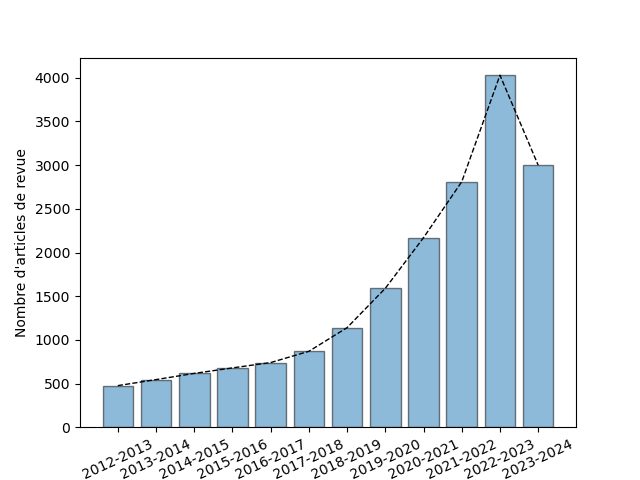
\includegraphics[width=0.8\textwidth]{paper_published}
	\caption{Nombre d'articles de revues recensés sur \textit{Google Scholar} avec les mots clés \og \textit{machine learning, retina} \fg.}
	\label{fig:articlesPublies}
\end{figure}


Cet engouement est en réalité fort logique car la rétine est un tissu particulièrement propice à la recherche informatique. En effet, l'imagerie rétinienne est (en général) non invasive et relativement peu onéreuse. Cela facilite la collecte et le partage des données à large échelle et donc la communion des efforts de recherche. Plus généralement, un bon nombre de diagnostic de pathologies rétiniennes s'appuie sur la lecture et l'interprétation d'image: or la vision par ordinateurs s'est dotée de nombreux nouveaux outils puissants sur la dernière décennie. L'engouement autours de la détection automatique de pathologies rétiniennes était donc prévisible. 
Cependant, cette récente prolifération des savoirs ne signifie pas la résolution de tous les obstacles qui jalonnent le chemin entre le laboratoire où est conçu l'algorithme  et le chevet du patient. Deux problèmes, parmi d'autres, reviennent régulièrement:
\begin{itemize}
	\item Quelle garantie existe-t-il de l'efficacité d'un algorithme une fois celui-ci sorti de l'univers calibré du laboratoire et appliqué au monde clinique? Autrement dit, comment garantit-on ses performances? Cette question s'inscrit dans le contexte de la \textbf{généralisation}.
	\item Comment encourager l'acceptabilité clinique d'un dispositif automatique? Un algorithme peut-il obtenir la confiance du clinicien ou du patient, de son concepteur ou des autorités de santé? Ce questionnement est au c\oe{}ur de tout un pan de la recherche dédié à l'\textbf{interprétabilité} des modèles. 
\end{itemize}
C'est sous le prisme de ces deux notions que s'inscrit ce doctorat. Cette recherche a évolué au fil du temps et au gré des collaborations entre les équipes d'ophtalmologie et de recherche de l'hôpital Maisonneuve-Rosemont de Montréal et du laboratoire LIV4D de l'École Polytechnique. Bien que l'application clinique soit toujours en ligne de mire, nos travaux s'inscrivent résolument dans le champs de l'apprentissage machine et le développement de nouveaux concepts fondamentaux. Pour cette raison, nous n'avons pas cantonné nos expériences à une seule modalité d'imagerie ni à une maladie spécifique. Au contraire, quand cela était possible, nous avons pris le parti d'exploiter les plus grandes collections de données possibles pour éprouver nos propositions théoriques sur les deux thématiques de généralisation et d'interprétabilité. Ce n'est donc pas la conception et le développement d'un seul modèle très spécialisé que présente cette thèse, mais les questionnements théoriques et pratiques auxquels un tel modèle se doit de répondre. À ces questionnements et dans la lignée de la littérature, nous proposerons des hypothèses de réponses et leur vérification. Ainsi, traiter de plusieurs maladies et de multiples modalités nous permet d'élargir la portée de nos conclusions. La structuration de ce document suivra cette logique: bien qu'il existe un fil conducteur entre elles, nos contributions méthodologiques peuvent se lire indépendamment les unes des autres. Mais avant de les présenter, le reste de la présente introduction vise à fournir les éléments de contexte permettant de familiariser le lecteur aux notions traitées.


\section{Éléments de la problématique}  % environ 3 pages
\subsection{Contexte anatomique et clinique}

Pour saisir les différents composantes de notre problématique, il est important de s'appuyer sur le contexte dans lequel s'inscrit ce doctorat. La recherche sur l'imagerie médicale impose un certain nombre de contraintes spécifiques: 
\begin{itemize}
	\item L'interprétation d'une image ne peut se faire sans faire sans un minimum d'expertise sur la structure anatomique imagée. La collaboration avec les médecins est donc souvent indispensable, en particulier pour l'annotation des données qui ne peut se faire sans leur contribution. 
	\item Plus pragmatiquement, la collecte des données est en général plus ardue que sur d'autres domaines. Plusieurs facteurs l'expliquent: le respect du consentement éclairé du patient est impératif et l'approbation par comité éthique avant collecte rajoute des étapes protocolaires. Chaque acquisition est donc coûteuse en temps ou en moyens (pour le patient et les équipes médicales en charge).
\end{itemize}
À la différence peut-être d'autres applications du \textit{Big Data}, ces contraintes rendent chaque donnée individuelle très précieuse. Il est donc important pour quiconque la manipule -y compris le chercheur en informatique- de comprendre a minima les bases anatomiques de la structure imagée, les contraintes physiques liées à la modalité d'acquisition et la manifestation des pathologies qu'on souhaite pouvoir détecter. Cette section se consacre donc à détailler ces différents points.

\subsubsection{Structure de l'\oeil.}

L'\oeil{} transforme la lumière reçue en influx nerveux qui sont transmis au cerveau. Tout comme un appareil photographique ne peut être réduit à un simple capteur photonique, l'\oeil{} est constitué d'un ensemble sophistiqué de tissus venant guider la lumière vers la rétine. Dans son apparence externe et à l'\oeil{} nu, le globe oculaire se compose de la sclère (\og blanc de l'\oeil{}\fg{} ) et de la cornée. La sclère est une structure résistante, visant à protéger l'\oeil{} des dégâts mécaniques. Elle est recouverte (hormis sur sa partie antérieure) par la conjonctive, responsable de la production du mucus intégrant la composition du liquide lacrymal. Sur sa partie antérieure, la sclère est percée pour laisser place à la cornée. Il s'agit d'une membrane circulaire bombée et transparente constituée à 78\% d'eau. Les larmes produites par les glandes lacrymales viennent l'alimenter en permanence et sont réparties sur toute sa surface par le battement des paupières. Elle est la principale responsable de la focalisation des rayons lumineux pénétrant l'\oeil{}: à elle seule, elle assure près de 80\% de la réfraction. Derrière la cornée se trouve une ouverture, nommée pupille, fonctionnant comme un diaphragme. La largeur de la pupille, contrôlée par les muscles lisses de l'iris, permet d'adapter la quantité de lumière pénétrant l'\oeil{}. \\
Pour assurer une mise au point aussi bien sur des objets lointains que proches, la focalisation doit être dynamique. Cette dynamique est rendue possible grâce au cristallin, petit disque fibreux situé à l'arrière de la cornée. La tension du cristallin est contrôlée par le corps ciliaire, constitué d'un réseau de muscles (muscles ciliaires) et également responsable de la sécrétion de l'humeur aqueuse. L'ensemble cornée/cristallin joue le rôle de doublet optique dont la longueur focale est régulée par la tension appliquée au cristallin.
Derrière ce dernier se trouve le corps vitré, où circulent les rayons lumineux avant de converger vers la surface tapissant l'intérieur du globe oculaire. Cette dernière, appelée rétine, est responsable de la conversion électromagnétique du signal lumineux en impulsions nerveuses. 


\subsubsection{Anatomie  de la rétine}
\label{sec:AnatRetina}
La vision humaine est le résultat de l'interaction complexe entre la lumière et des photorecepteurs qui convertissent et envoient les signaux nerveux au cerveau. Le siège de cette interaction se trouve dans la rétine, tissu qui tapisse la surface interne de l'\oeil. Au cours de l'embryogènese, la rétine se développe depuis la cupule optique (tête du nerf optique), une excroissance issue du cerveau frontal \cite{willoughbyAnatomyPhysiologyHuman2010}. De cette tête de nerf optique émergera le réseau vasculaire chargé d'irriguer l'ensemble des couches de la rétine; il est compris d'artères, de veines et de micro-vaisseaux nommés capillaires rétiniens. En ce qui concerne les couches rétiniennes, elles se distinguent par le type de neurones qui les composent. Il en existe cinq classes majeures dans la rétine: les photorécepteurs, les cellules bipolaires, les cellules horizontales, les cellules amacrines et les cellules ganglionnaires. Sur des coupes histologiques, on peut en dénombrer un nombre plus important encore et observer précisément l'organisation en couches de ceux-ci.
Radialement (en suivant le chemin de la lumière  arrivant dans l'\oeil), ces couches rétiniennes superposées sont:
\begin{enumerate}
	\item La membrane limitante interne, composée des cellules de Müller.
	\item La couche des fibres nerveuses, c'est à dire les axones des cellules ganglionnaires. 
	\item La couche des cellules ganglionnaires, qui contient leurs noyaux.
	\item La couche plexiforme interne formée des cellules amacrines
	\item La couche nucléaire interne formée des cellules bipolaires
	\item La couche plexiforme externe formée des cellules horizontales
	\item La couche nucléaire externe, où se situent les photorécepteurs (cônes et bâtonnets).
	\item L'épithélium pigmentaire (ou RPE pour \textit{Retinal Pigment Epithelium}), par où se font les échanges nutritifs et apports sanguins entre la rétine et les structures plus profondes.
\end{enumerate}
Sous cette dernière couche se trouve un second tissu, appelé la choroïde. C'est par celle-ci, très vascularisée, que se fait la nutrition de l'iris et des photorécepteurs. Parmi ceux-ci, la distinction entre cônes et bâtonnets permet d'expliquer la vision en couleur et et la vision périphérique. Tout comme la plupart des vertébrés, l'être humain possède ces deux types de cellules, les bâtonnets étant près de vingt fois plus nombreux que les cônes (on compte entre 110 et 130 millions de bâtonnets pour environ 7 millions de cônes). 
Les cônes sont responsables de la perception de la couleur. Ils contiennent différents pigments réagissant respectivement à trois plages de longueurs d'onde en envoyant un influx nerveux au cerveau. Ces longueurs d'ondes correspondent à peu près au bleu, au vert et au jaune sur le spectre de la lumière. Les bâtonnets pour leur part ne disposent que d'un type de pigment, sensible aux longueurs d'onde proche du bleu; ils sont par conséquent incapable de distinguer les couleurs. En revanche, étant plus sensibles, ils restent actifs même en faible luminosité. Chez l'humain, près de 50\% des cônes sont situés au sein d'une structure centrale appelée macula, au centre de laquelle se trouve la fovéa, point central concentrant la majorité des cônes. 
\\
La macula est donc le point central de la vision. Il s'agit d'une région elliptique de \SI{1,5}{\milli\meter} de large pour \SI{1}{\milli\meter} de hauteur. Au niveau de la fovéola (centre de la fovéa), elle est très mince (\SI{130}{\micro\meter}). La région dépressionnaire de la fovéola est bordée par une structure en bourrelet nommée clivus, d'une épaisseur de \SI{410}{\micro\meter}. Ailleurs, l'épaisseur moyenne de la rétine varie entre \SI{180}{\micro\meter} à l'équateur et va en diminuant sur la périphérie (jusqu'à \SI{100}{\micro\meter}). Ces différentes structures sont visibles par des coupes histologiques ou in vivo par l'imagerie de \fundus{} et de la \ac{OCT}.
\\
Cette brève description de la rétine va nous permettre d'introduire les deux grandes pathologies pouvant l'affecter et les manifestions cliniques que celles-ci déclenchent. Mais auparavant, nous ouvrons une brève parenthèse sur les modalités permettant d'imager la rétine.

\subsubsection{Modalités d'acquisition de l'imagerie rétinienne}
La photoréception se faisant dans la rétine, celle-ci possède intrinsèquement une propriété particulièrement propice à l'imagerie: en effet, si les rayons lumineux se focalisent en son sein, il est possible de leur faire parcourir le chemin inverse pour reconstruire une image de celle-ci. L'observation de la rétine peut donc se faire de manière non invasive (c'est-à-dire sans injection d'agents de contraste, sans radiation ni opération chirurgicale). \\
De nombreuses modalités ont été développées pour la visualiser. Nous en fournissons une description plus détaillée en annexe \ref{sec:ImagerieRetina}, mais en résumé dans le cadre de cette thèse, nous nous sommes concentrés sur les deux principales:
\begin{itemize}
	\item L'imagerie de \fundus{}, qui consiste en une photographie en couleurs de la surface rétinienne. Une acquisition de \fundus{} est aisée, peu coûteuse et haute résolution. Ces propriétés la rendent très populaire dans le cadre de programme de dépistage à large échelle.
	\item La \acf{OCT}. Cette forme d'imagerie repose sur le principe de l'interférométrie et permet d'obtenir une estimation de la profondeur des différentes interfaces rétiniennes selon un axe: cette représentation 1D est appelée A-scan. En balayant cet axe le long d'une ligne, on obtient une image 2D appelée  B-scan que l'on peut comparer à une vue en coupe de la rétine. En déplaçant l'axe de coupe, on obtient une succession de B-scan formant un volume: l'OCT permet ainsi d'obtenir une représentation tri-dimensionnelle de la rétine.
\end{itemize}

\subsubsection{Pathologies rétiniennes et contexte clinique}
Il existe un très grand nombre de maladies rétiniennes, aussi bien susceptibles de n'affecter que la rétine que d'être le symptôme d'une pathologie systémique. Une énumération exhaustive de celles-ci n'est pas le propos de cette section, nous nous contenterons ici d'une brève synthèse sur les deux principales maladies affectant la rétine. Le choix de ces maladies est dicté par deux considérations:
\begin{enumerate}
	\item Leur prévalence et incidence respectives, qui en font des maladies de première importance en terme de santé publique.
	\item En conséquence, l'effort déployé ou ambitionné pour aboutir à des campagnes de dépistage à plus ou moins large échelle. Pour arriver à cette fin, l'intégration des nouvelles technologies (que ce soit d'acquisition, de télémédecine ou d'analyse automatique) fait consensus. Cela justifie donc d'y prêter une attention toute particulière.
\end{enumerate}

Par volonté de concision, nous avons ici synthétisé les principales informations concernant les maladies, mais plus de détails sont donnés pour chacune en annexe \ref{sec:MaladiePrevalence}. Nous y avons également ajouté une section dédiée au glaucome en raison de sa forte prévalence; cependant nos travaux n'ont pas de lien direct avec cette maladie.
\paragraph{La rétinopathie diabétique}
La \ac{RD} est la principale cause de déficience visuelle au sein de la population adulte en âge de travailler. 
Elle se développe en conséquence d'une complication répandue du diabète sucré. Ce dernier est lui-même causé par une défaillance des mécanismes de régulation de la glycémie entraînant une hyperglycémie. Or, un taux élevé de glucose dans le sang occasionne des dommages sur les petits et gros vaisseaux sanguins. La cible principale du glucose est l'endothélium (tissu constituant la paroi interne des vaisseaux, formée de cellules épithéliales) et la lame basale (sur laquelle repose les cellules épithéliales et chargée des apports nutritifs à l'endothélium). Un taux élevé de glucose et d'insuline dans le sang peut avoir pour conséquence de modifier les réactions des cellules de l'endothélium et d'augmenter la viscosité du sang, modifiant ainsi chimiquement certaines protéines. Dans le cas de la rétine, ces effets peuvent entraîner deux types de réactions:
\begin{itemize}
	\item Une ischémie, que l'on définit comme la diminution de l'apport sanguin artériel à un organe, généralement du fait d'une obstruction de l'artère. Dans la rétine, cette obstruction peut conduire à la croissance de néo-vaisseaux pouvant entraîner des saignements et causer un détachement rétinien. Si ce stade est atteint, on parle alors de \ac{RD} proliférative.
	\item La rupture de la barrière hématorétinienne. Le liquide exsudé peut provoquer un enflement de la macula et endommager les photorécepteurs. Cette complication a pour nom un \ac{OMD}.
\end{itemize}
L'ischémie peut causer un blocage du transport axonal (déplacement de mitochondries, lipides, protéines et autres cellules dans le corps du neurone, permettant le renouvellement de celui-ci). L'accumulation axoplasmique dans la couche des fibres optiques entraîne des lésions appelées nodules cotonneux, d'apparence blanche et aux frontières floues. \\
Cliniquement, les premiers signes de \ac{RD} sont l'apparition de microanévrismes et d'hémorragies intrarétinales. À un stade plus avancé de la maladie, la rétine s'épaissit (formation d'un \oe{}dème) et des exsudats (dépôts de lipides) apparaissent pouvant causer une perte d'acuité visuelle. Si la progression de la maladie se poursuit, elle peut atteindre le stade prolifératif, dont le nom provient de l'apparition de nouveaux vaisseaux dans le disque optique, la rétine ou l'iris. Ces néo-vaisseaux ont pour conséquence potentielle un détachement rétinien ou un glaucome néovasculaire. C'est à ce stade que le risque de perte totale de la vision est le plus important.

\paragraph{La Dégénérescence Maculaire Liée à l'Age}
\label{sec:DMLADescription}
Comme son nom l'indique, la \ac{DMLA} est une maladie affectant la macula. Elle est la principale cause de cécité chez les personnes âgées de plus de 50 ans dans les pays développés. Comme la \ac{DMLA} se concentre dans la région maculaire, cette cécité est rarement complète car elle n'affecte pas la vision périphérique. Les causes de la maladie restent mal connues, mais sont suspectées d'être polygéniques, incluant des facteurs de risques environnementaux (tabagisme, surpoids). Il existe deux formes de \ac{DMLA}: la première, dite sèche, correspond à une atrophie de la macula et représente la très vaste majorité des cas. La seconde, dit exsudative ou humide, correspond à l'apparition de néovascularisation choroïdienne. Bien que plus rare, elle évolue beaucoup plus rapidement que la première.
La majeure partie des symptômes que nous synthétisons ici provient des travaux de Kolar et. \cite{kolarClassificationClinicalFeatures2013}. 

La \ac{DMLA} se caractérise par l'un (ou plusieurs) des symptômes suivants:
\begin{itemize}
	\item La présence de drusens de taille intermédiaire. Un drusen est une lésion d'apparence jaune plus ou moins contrastée. Histologiquement, ils sont situés au niveau de l'interface avec l'\ac{RPE}. Une taille intermédiaire correspond à une taille comprise entre \SI{63}{\micro\meter} et \SI{125}{\micro\meter}. 
	\item Des anomalies de la \ac{RPE}, en particulier de l'hypopigmentation ou de l'hyperpigmentation. L'hypopigmentation est associée à un amincissement de la \ac{RPE} et en conséquence à un plus faible taux de mélanine.  L'hyperpigmentation quant à elle est une conséquence d'une migration ou d'une prolifération des cellules de la \ac{RPE} vers les couches supérieures (dans la direction de la surface de la rétine)
	\item La présence de pseudodrusen réticulaire. Il s'agit de dépôts de matière situés dans les couches supérieures à la \ac{RPE}.
	\item La présence d'un ou plusieurs des marqueurs suivants: une atrophie géographique de la \ac{RPE} -qui laisse apparaître la choroïde voire même de la sclère à l'imagerie de \fundus{}-, une néovascularisation choroïdale, des traces de prolifération angiomateuse rétinienne (\textit{Retinal Angiomatous Proliferation}) -en simplifié, une néovascularisation démarrant depuis la rétine.  
\end{itemize}

\subsection{L'Apprentissage Machine appliqué à la rétine}
L'engouement croissant pour les algorithmes de reconnaissance d'image a trouvé de nombreux échos dans la recherche liée à l'imagerie rétinienne, en particulier pour traiter des deux maladies présentées précédemment. Plusieurs solutions logicielles développées par des acteurs privés ou publics ont d'ors-et-déjà reçu une autorisation de mise sur le marché par les organismes de régulation sanitaire Américain et Canadien. Ces accréditations sont pour la plupart très récentes (2018 pour la plus ancienne) mais ce marché en forte croissance attire régulièrement de nouveaux acteurs \cite{pressAIDiabeticRetinopathy, EyenukAnnouncesFDA2020}.
Tous les systèmes ne sont pas équivalents, les plus complets permettent d'obtenir une évaluation de la qualité de l'image acquise, la détection de la rétinopathie diabétique (stade modéré ou pire), la présence d'éléments témoignant de \ac{DMLA} ou encore des dommages dans la tête de nerf optique signes de glaucome. Si les acteurs qui développent ces solutions revendiquent généralement des performances en général très élevées (de paire avec celle d'un médecin), un certain nombre d'interrogations sont régulièrement soulevées quant au fonctionnement des modèles utilisés. La principale critique émise à leur encontre concerne leur fonctionnement dit \og en boîte noire \fg: le modèle est capable de prédire correctement un diagnostic, mais l'utilisateur (médecin, patient ou même le concepteur du modèle) est dans l'incapacité de comprendre ce qui a guidé la machine dans son choix. Cet aspect est souvent cité comme un frein à l'adoption clinique de ces systèmes. Plus généralement, la faculté d'un algorithme à expliquer son \og raisonnement \fg est un problème ouvert; il a donc occupé le c\oe{}ur de ce doctorat. Or, les maladies rétiniennes que sont la DMLA et la rétinopathie diabétique sont toutes deux diagnostiquées à partir de lésions locales répondant à des descriptions précises. L'identification de celles-ci (opération appelée segmentation sémantique), préalablement au diagnostic, apparaît donc comme une étape vers une meilleure compréhension du modèle de classification de la maladie. Malheureusement, la segmentation sémantique ne peut se faire qu'avec des données annotées précisément par des médecins et 
celles-ci sont rares et coûteuses à rassembler. Plus problématique encore, les protocoles d'annotations varient fortement en fonction des bases de données à disposition publiquement. Bien que celles-ci soient très utilisées pour concevoir et valider des modèles, l'effet de cette hétérogénéité est peu analysé. Nos propres travaux sur la segmentation sémantique s'inscrivent donc en partie dans le cadre d'une étude approfondie sur la notion sous-jacente de généralisation. \\
Un second aspect que nous abordons est celui de la classification des images à partir des cartes de segmentation obtenues. La littérature s'interroge peu sur la relation entre la qualité de la segmentation et la performance de classification; cette question reste donc à aborder.
\\
Il existe cependant une alternative à la segmentation qui permette d'utiliser directement un modèle de classification tout en explicitant ses mécanismes de fonctionnement internes. En effet, dans une certaine mesure, il est aujourd'hui possible d'expliquer le fonctionnement d'un modèle. Une telle étude relève du champs de l'interprétabilité. S'il existe de nombreuses façons d'aborder cette question, celle qui nous intéressera a trait à la notion de cartes d'attributions. Ces dernières jouent un rôle similaire à la segmentation sémantique: elles délimitent localement les zones d'intérêts dans l'image justifiant la prédiction du modèle. Ces cartes ont l'avantage de ne pas nécessiter d'annotations locales, précisément celles coûteuses à obtenir. Malheureusement, les divers algorithmes d'attributions existants sont loin de générer des annotations de la précision et de la résolution d'une réelle segmentation, elles ne peuvent donc prétendre à les substituer en l'état.
\\
Enfin, au-delà des performances mesurées sur des métriques (qui peuvent être elles-même problématiques), l'applicabilité des algorithmes développés pose aussi question. Dans un environnement où des solutions logicielles sont déjà commercialisées, quelle place reste-t-il à des outils de recherche qui rivalisent difficilement sur ces métriques?
Cette question naît du constat que dans la vaste majorité des travaux publiés dans le domaine, les conclusions ne s'étendent guère au delà du report de scores de performances sur des bases de référence. L'utilisatibilité de ces algorithmes, que ce soit à des fins de recherche ou de déploiement clinique est donc souvent laissée en suspens. 
%%
\section{Objectifs de recherche}  % 0.5 page


Au vu des différents éléments de la problématique, nous nous sommes fixés deux axes principaux de recherche. Le premier, dédié au \fundus{} et à la segmentation, est bâti autours des objectifs de recherche suivants:
\begin{itemize}
	\item Caractériser les bases de données publiques dédiées à la segmentation de l'imagerie de \fundus{} (plus spécifiquement des lésions).
	\item Concevoir un modèle de segmentation sémantique automatique capable de détecter les lésions rétiniennes sur différentes bases de données tout en atteignant les performances reportées dans l'état de l'art.
	\item Analyser les conséquences de l'hétérogénéité des données sur l'entraînement et la validation du modèle puis expérimenter des stratégies permettant de les modérer voire de les contrôler.	
	\item Construire un modèle de détection de la rétinopathie diabétique dans le \fundus{} basé uniquement sur les cartes de lésions et les comparer avec les approches traditionnelles.
\end{itemize}
Le second axe de recherche explore la deuxième partie de notre problématique, à savoir l'interprétabilité des modèles. Pour cela, nous avons établi les objectifs suivants:
\begin{itemize}
	\item Comparer les architectures convolutives traditionnelles aux récents modèles de type auto-attentifs (plus particulièrement les \textit{Vision Transformer} \cite{dosovitskiyImageWorth16x162020}) à des fins de classification du \fundus{} et de l'OCT. 
	\item Étudier les algorithmes de génération de cartes d'attributions existants et proposer une approche permettant d'affiner celles générées par le modèle ViT.
	\item Comparer qualitativement et quantitativement les cartes d'attributions. Pour l'aspect quantitatif, nous utiliserons les annotations de segmentation faites par des cliniciens.
	\item Impliquer les médecins dans l'évaluation de l'utilité des différentes cartes d'attributions et donc proposer un protocole de collaboration permettant de recueillir leur contribution de manière efficace et non-biaisée.
\end{itemize}
\section{Plan de la thèse}  % 0.5 page
Pour contextualiser nos travaux au sein de la littérature existante, le prochain chapitre présente l'état de l'art propre à notre domaine. Nous l'avons organisé en deux parties distinctes. La première, très généraliste, introduit certaines notions fondamentales de l'apprentissage profond. Son contenu s'adresse avant tout au lecteur peu familier des avancées du domaine obtenues lors des dix dernières années. À partir de la section \ref{sec:NoisyLabelLearning}, nous focaliserons notre revue sur les travaux liés à notre domaine, en couvrant dans l'ordre les questions de généralisation, d'interprétabilité, de mesure de performances et les applications à l'ophtalmologie de tous ces points. \\
Les chapitres qui suivent cet état de l'art s'organisent peu ou prou dans l'ordre des objectifs de recherche que nous nous sommes fixés. Le chapitre \ref{sec:Theme1} traite de la segmentation sémantique dans l'imagerie de \fundus{}. Nous y proposons une comparaison pléthorique de modèles entraînés sur diverses bases de données, elles-même préalablement caractérisées en terme de qualité d'images et d'annotations. L'hétérogénéité des bases de données y sera étudiée et en particulier, nous y discuterons du comportement inattendu qu'elles peuvent engendrer. Cette observation aboutira au développement d'une stratégie originale de conversion des données dite \og adversariale \fg permettant de changer de style d'annotations sans altérer un réseau entraîné.
Dans un second temps, ce même chapitre introduira une nouvelle manière de classifier les images de \fundus{} s'appuyant sur une représentation par graphe de celle-ci. Cette contribution originale a pour objectif de quantifier la qualité de la segmentation au travers des performances de classification et nous montrons qu'en cela, elle se distingue significativement des travaux existants. \\
Le chapitre \ref{sec:Theme2} se consacre à la question de l'interprétabilité; nous y introduirons pour cela divers modèles entraînés sur des bases de \fundus{} et d'OCT. Un intérêt tout particulier est consacré aux modèles de type ViT. En effet, au cours de nos expériences, la découverte d'un mécanisme de ré-échantillonnage des séquences d'entrées du dit modèle nous amènera à exploiter des capacités insoupçonnées de ce dernier et à améliorer ses performances sans avoir à le ré-entraîner. Toujours dans l'optique de fournir des diagnostics transparents pour le médecin et en s'appuyant sur cette découverte, nous introduirons le principe d'Attention Concentrée, qui nous permet de générer des cartes d'attributions hautes résolutions. \\
Le chapitre \ref{sec:Theme3} propose de revenir sur les algorithmes conçus au cours de la thèse sous la forme d'une discussion sur leur applicabilité. Pour cela, nous avons choisi d'orienter cette discussion sous la forme d'une présentation succincte de diverses expériences cliniques menées au cours de cette thèse utilisant les algorithmes développés. Les méthodologies mises en place et les résultats obtenus n'y sont que brièvement mentionnés car nous prenons le parti pris de privilégier une discussion sur les forces et faiblesses de nos différentes contributions à la lumière d'applications cliniques bien réelles.



       % Introduction au sujet de recherche.
\Chapter{REVUE DE LITTÉRATURE}\label{sec:RevLitt}




La recherche informatique appliquée à l'imagerie médicale se trouve à l'intersection de deux domaines et a par conséquent deux objets d'études: la conception d'algorithmes novateurs et la validation de ceux-ci suivant un protocole simulant un déploiement clinique. Les fondations de ce champs de recherche reposent donc à la fois sur des théories mathématiques statistiques et sur des considérations plus empiriques portant sur l'efficacité et l'utilisabilité des algorithmes dans un contexte clinique. Pour introduire notre recherche, on ne peut faire abstraction d'une description des emprunts faits à l'apprentissage machine et aux statistiques en général, emprunts réalisés non sans de nécessaires (et parfois substantielles) adaptations. \\
Afin de faciliter la compréhension du lecteur non initié, cette revue de littérature s'ouvre sur une introduction des principes théoriques constituant les briques fondamentales de la reconnaissance automatique d'images par apprentissage profond. Ainsi, les sections allant de \ref{sec:IntroductionVisionOrdinateur} à \ref{sec:interpretationProbabiliste} ont essentiellement une visée pédagogique. Les algorithmes qui y sont mentionnés appartiennent à la trousse à outils du chercheur, leur application n'est pas spécifique à un domaine en particulier. Nous y couvrons les opérateurs fondamentaux sur lesquels se basent les réseaux de neurones, un survol historique des architectures qui ont marqué ces dix dernières années (dont plusieurs réapparaîtront dans nos expériences) et un rappel sur les méthodes d'entraînement de celles-ci.
\\
À partir de la section \ref{sec:NoisyLabelLearning}, nous concentrons notre revue de littérature sur les éléments qui occupent le cœur de cette thèse: ainsi, dans la  section \ref{sec:theorieApprentissage}, nous introduirons le concept de généralisation et les éléments statistiques qui appartiennent à ce domaine. Cette présentation est découpée en une première introduction théorique suivie de considérations plus empiriques sur les questions d'adaptation de domaines et d'apprentissage sur cible bruitée. 
\\
La section \ref{sec:interprétabilitéModel} présente les notions d'explicabilité et d'interprétabilité des modèles, c'est-à-dire la compréhension qu'un utilisateur humain peut avoir de leur fonctionnement. Plus spécifiquement, nous nous concentrons sur le champs de recherche dédié aux méthodes de génération d'attribution locale.
\\
Enfin, à partir de la section \ref{sec:RevueLittOphtal}, nous aborderons plus spécifiquement les applications propres à l'ophtalmologie des modèles d'apprentissage machine, en discutant de la segmentation sémantique de lésions du \fundus{} et des approches locale et globale de classification par maladie.
\section{Réseaux de neurones dédiés à la vision par ordinateur}
\label{sec:IntroductionVisionOrdinateur}
\subsection{La trousse à outils numérique de l'apprentissage profond}

L'apprentissage machine est un champs englobant de nombreux concepts et algorithmes inventés au fil du développement de l'informatique. S'il ne fallait leur trouver qu'un seul point commun, ce serait de s'appuyer sur un ensemble de données observées pour construire une représentation statistique des relations qui régissent ces données. En cela, l'apprentissage machine se distingue des modélisations mathématiques ou physiques plus traditionnelles car il ne cherche pas à identifier explicitement les mécanismes de cause à effet; mais plutôt à dévoiler les corrélations statistiques qui expliquent au mieux les données observées. L'hypothèse qui prévaut est que si l'observation est suffisamment exhaustive, le modèle statistique s'approchera au plus près de la loi réelle qui régit le phénomène observé. \\
Dans ce vaste univers qu'est l'apprentissage machine, nous n'aborderons directement qu'une sous-catégorie, dite de l'apprentissage profond. Celle-ci a largement accaparé les devants de scènes scientifiques mais aussi médiatiques. Il faut noter que ses contours ne sont pas forcément unanimement définis, mais la grande majorité des travaux qui se revendique de l'apprentissage profond repose sur une forme plus ou moins évoluée de réseaux de neurones. 
Afin d'introduire ce domaine, nous souhaitons définir en premier lieu les grandes briques fonctionnelles utilisées par les réseaux de neurones. Les deux prochaines sous-sections sont donc à aborder comme une sorte de lexique simplifié; ce n'est qu'à partir de la section \ref{sec:ReseauxNeurones} que nous rentrerons dans les détails de la littérature sur le sujet.

\subsubsection{Le neurone formel}
Dans sa conception originale, le neurone formel s'inspire de son équivalent biologique: ce dernier possède plusieurs dendrites (modélisées comme des entrées) et un axone (modélisé comme une sortie). Les dendrites reçoivent un influx nerveux en provenance d'autres neurones (plus exactement de leur terminaison axonale) au niveau des synapses: ces influx sont modélisés sous forme de signaux numériques. L'opération réalisée par le neurone est modélisée comme une somme pondérée de ses entrées, puis, si cette somme franchit un certain seuil, sa transmission à sa sortie. Ainsi, dans sa forme la plus épurée, le neurone formel à $N$ entrées réalise simplement l'opération suivante:
\begin{equation}
	\label{eq:NeuroneFormel}
	y = \sigma(\sum_{i = 1}^N x_i w_i + b)
\end{equation}
où $\mathbf{x} \in \mathbb{R}^N$ est son entrée et $y \in \mathbb{R}$ sa sortie.
L'opérateur $\sigma$ représente une fonction de seuil, aussi dite d'activation. Elle est non-linéaire et distingue le neurone formel d'une simple projection linéaire. Les paramètres $\mathbf{w} \in \mathbb{R}^N$ et $b \in \mathbb{R}$ (appelés respectivement poids et biais) sont ses variables d'ajustemement qui, modifiées en fonction de l'objectif visé, permettent au neurone de produire la sortie attendue et donc \og d'apprendre \fg. L'équation \ref{eq:NeuroneFormel} peut se réécrire de manière équivalente sous sa forme vectorielle: $y = \mathbf{w}^T\mathbf{x} + b$. \\
En pratique, on n'utilise jamais un seul neurone isolé mais plutôt une couche de neurones (qui n'est rien d'autres que le calcul parallèle de $M$ neurones). Avec $\mathbf{x} \in \mathbb{R}^N$, $\mathbf{y} \in \mathbb{R}^M$, $\mathbf{b} \in \mathbb{R}^M$ et $\mathbf{W} \in \mathbb{R}^{N\times M}$, l'équation d'une couche neuronale s'obtient de manière similaire à celle de l'équation \ref{eq:NeuroneFormel}:
\begin{equation}
	\label{eq:CoucheNeuroneFormel}
	\mathbf{y} = \sigma(\mathbf{W}^T\mathbf{x} + \mathbf{b})
\end{equation}

Enfin, revenons sur la fonction d'activation $\sigma$: de nombreuses propositions existent dans la littérature, nous en recensons quelques unes sur la figure \ref{fig:activations_functions}. Elles modélisent en général un effet de saturation (limite finie vers $+/- \infty$), qui s'interprète comme un seuil au delà duquel le neurone s'active.
\begin{figure}[htb]
	\centering
	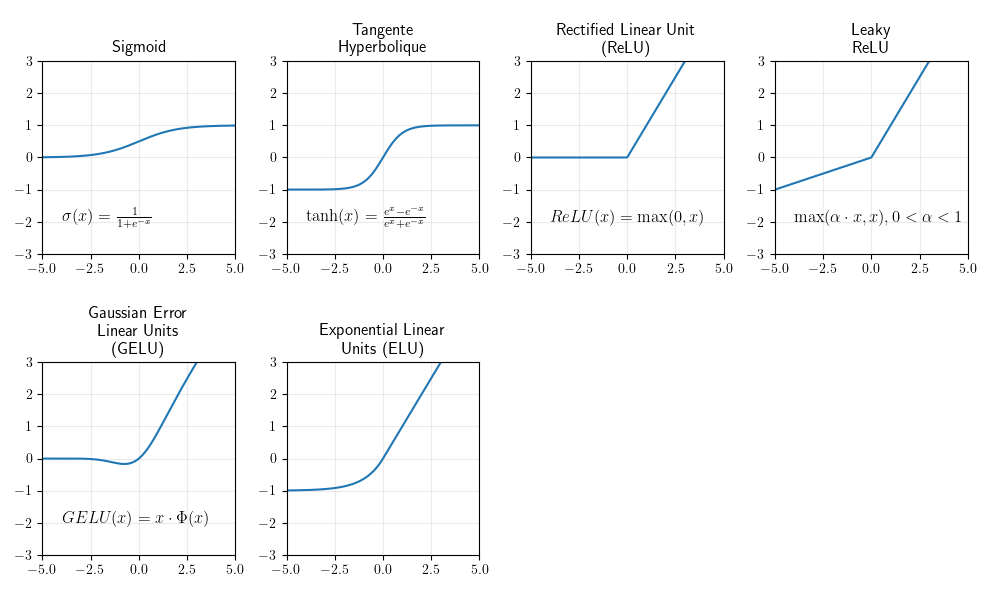
\includegraphics[width=\textwidth]{revue_litterature/activation_functions.png}
	\caption{Fonctions non-linéaires usuelles placées en sortie de neurones}
	\label{fig:activations_functions}
\end{figure}

\subsubsection{Le réseau de neurones multicouches}
En ayant introduit le neurone formel et son corollaire, la couche de neurones, nous disposons des bases nécessaires pour définir le premier réseau de neurones, dit multicouches. Son principe est simple: à l'instar du cerveau et son imbrication complexe de neurones, il est possible d'organiser un réseau artificiel sous la forme d'une succession de couches, connectées les unes aux autres de manière séquentielle. Autrement dit, la sortie de la couche $l$ est fournie en entrée de la couche $l+1$. Pour chacune, l'équation \ref{eq:CoucheNeuroneFormel} est respectée, même si chaque couche peut disposer d'une fonction d'activation qui lui est propre. Ce faisant, un réseau peut s'interpréter comme une composition (au sens mathématique) alternant projection linéaire et non-linéarité via la fonction d'activation:
\begin{equation}
	\mathbf{y} = \mathcal{F}(\mathbf{x}) = (\sigma^{(L)} \circ f^{(L)}) \circ ...\circ(\sigma^{(l)} \circ f^{(l)}) \circ ... \circ(\sigma^{(0)} \circ f^{(0)})(\mathbf{x}) 
\end{equation}
Sémantiquement, toutes les couches d'indice $l \in \left\lbrace 0, 1, ..., L-1\right\rbrace $ sont appelées couches cachées et leur nombre $L$ est référé sous le terme de profondeur du réseau. Par analogie, on parle de largeur pour désigner le nombre de neurones par couche. Ces deux paramètres (largeur et profondeur) font partie des choix architecturaux à faire dans la conception d'un modèle. Depuis les années 80, l'expressivité de $\mathcal{F}$ (c'est-à-dire sa capacité à approximer n'importe quelle fonction) est largement étudiée, dépendamment de la largeur et de la profondeur choisies. Les travaux de Cybenko G. sont précurseurs en la matière: il y introduit un des Théorèmes d'Approximation Universelle, démontrant la capacité d'un réseau de profondeur $d=1$ (une couche cachée) utilisant la fonction sigmoïde à approcher n'importe quelle fonction dès lors que sa largeur est assez grande (possiblement infinie). Des versions plus modernes de ces travaux généralisent ce théorème à différents types de non-linéarité. Depuis les travaux de travaux de Zhou et al. \cite{luExpressivePowerNeural2017} la tendance récente est à promouvoir une largeur bornée et une profondeur accrue. Cai et al. \cite{caiAchieveMinimumWidth2023a} explicitent, sous certaines conditions, une borne minimale à la largueur nécessaire.

\subsubsection{Quelques autres opérateurs usuels}
Dans la trousse à outils du concepteur de réseaux de neurones, d'autres opérateurs reviennent très fréquemment, sans que leur paternité ne soit très clairement définie: c'est en particulier le cas du \textit{Pooling} et du \textit{Softmax} \footnote{Nous conservons dans cette thèse les termes anglais à défaut d'une traduction adoptée unanimement par la communauté francophone}.

\paragraph{Le Pooling}est une opération de sous-échantillonnage très simple: au sein d'une fenêtre donnée, il s'agit d'aggréger la sortie de plusieurs neurones en une seule valeur. En pratique, on utilise fréquemment de deux types de pooling:
\begin{itemize}
	\item Le \textit{Max-Pooling} qui consiste à prendre la valeur maximale parmi les neurones dans la fenêtre considérée.
	\item Le \textit{Mean-Pooling} qui effectue la moyenne des neurones dans cette fenêtre.
\end{itemize}
Il n'existe pas nécessairement de justification théorique sur l'utilisation de l'une ou l'autre des méthodes; on peut simplement noter que le Max-Pooling est nettement prévalent.
\paragraph{Le Softmax} est une opération de normalisation $f: \mathbb{R}^d  \mapsto \left[0, 1 \right]^d$ définie par:
\begin{equation}
	f(\mathbf{x}) = \frac{\exp(\mathbf{x})}{\sum_i \exp(\mathbf{x}_i)}
\end{equation}
Généralement appliqué en sortie de la dernière couche d'un réseau de neurone, le Softmax ramène toutes les valeurs des neurones dans un intervalle fermé $\left[0, 1 \right]$. Par ailleurs, il contraint la somme de ces neurones à valoir 1. Pour cette raison, la sortie d'un softmax s'interprète généralement comme une distribution discrète de probabilités.


\subsection{Réseau de Neurones Convolutifs}
\label{sec:ReseauxNeurones}
La conceptualisation et l'étude de nouvelles architectures de réseau de neurones ont constitué une majeure partie des publications récentes (période 2012-2023). Comme le formulent Alzubaidi et al., cet aspect de la recherche représente le noyau dur de l'\textit{Apprentissage Profond} \cite{alzubaidiReviewDeepLearning2021}.
\\
Nous mettons ici l'accent sur les principales avancées obtenues en reconnaissance automatisée dans le domaine de la vision par ordinateur, donc sur des images. Dans ce domaine et bien avant l'émergence des réseaux neuronaux, l'opérateur de convolution est reconnu comme une clé de voûte de bien des algorithmes de traitement d'image. Connue pour ses propriétés dans le domaine du filtrage, la convolution est réinterprétée par Le Cun et al. \cite{lecunGradientbasedLearningApplied1998} qui proposent de rendre son noyau entraînable par descente de gradients. Cette idée, sans être conceptuellement révolutionnaire, a une grande importance théorique et pratique. La convolution n'étant qu'une projection linéaire locale, son interprétation sous le prisme de la théorie du neurone formel est assez directe. L'idée fondamentale des auteurs est remplacer les premières couches de neurones classiques par des couches convolutives, décomposant ainsi le réseau en une première partie liée à l'extraction de caractéristiques locales et une seconde à l'aggrégation et la classification de celles-ci.
L'architecture résultante, appelée LeNet-5, devient donc le premier \ac{CNN} (Figure \ref{fig:lenet}). Elle est composée de 4 couches convolutives suivies d'un \ac{PMC} à deux couches. Dans le détail, chaque couche convolutive est constituée d'un ensemble de filtres, dont les sorties sont concaténées pour former un tenseur de cartes de caractéristiques. Formellement, notons $f^k$ la fonction réalisée par la couche convolutive $k$. Celle-ci est paramétrée par un vecteur de poids $\mathbf{W}^k \in \mathbb{R}^{I \times O \times M \times N}$ et de biais $\mathbf{B} \in \mathbb{R}^I$. Les dimensions $M \times N$ représentent la taille du noyau de convolution. Cette fonction reçoit un tenseur d'entrée $\mathbf{X}^k \in \mathbb{R}^{I \times H \times W}$ et produit en sortie un tenseur $\mathbf{Y}^k \in \mathbb{R}^{O \times H' \times W'}$ 
\begin{equation}
	\mathbf{Y}^k = f^k(\mathbf{X^k})
\end{equation}
L'équation détaillée d'une couche convolutive est donnée par:
\begin{equation}
	\mathbf{Y}^k[o, h, w] = \sum_{i=1}^{I}\sum_{m, n=1}^{M, N}\mathbf{X}^k[i, h +m - \lfloor M/2 \rfloor, w +n - \lfloor N/2 \rfloor] \cdot \mathbf{W}^k[i, o, m, n] + \mathbf{B}[i]
\end{equation}

%\begin{figure}[htb]
%	\centering
%	
\includegraphics[width=5in]{placeholder}
%	\caption{Description d'une opération de convolution au sein d'une couche convolutive}
%	\label{fig:convolution}
%\end{figure}

\begin{figure}
	\centering
	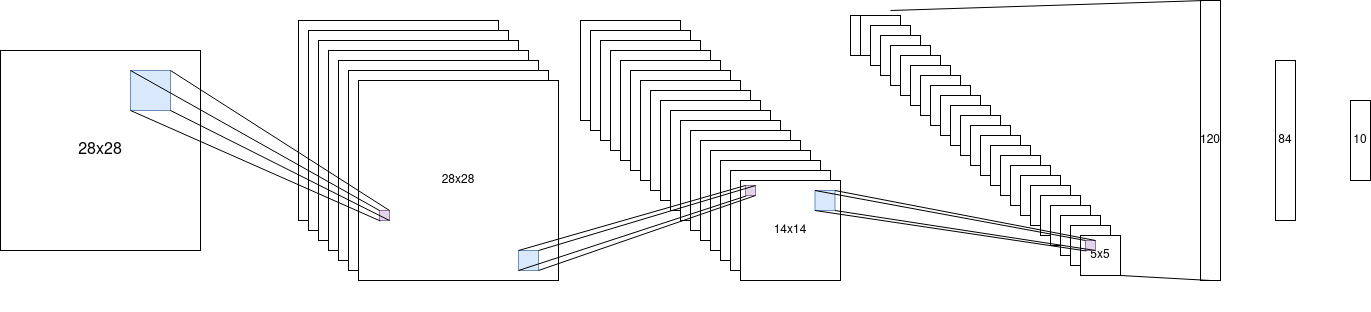
\includegraphics[width=0.7\textwidth]{gnuplot/revue_litterature/LeNet}
	\caption{Représentation simplifiée du réseau LeNet-4}
	\label{fig:lenet}
\end{figure}


La première dimension $I$ correspond aux canaux du tenseur d'entrée. Ainsi, $\mathbf{X}^0$ qui correspond à l'image d'entrée du réseau, possède généralement un ou trois canaux (monochrome, \og rouge, vert, bleu\fg) et $I \in \{ 1, 3\}$.  
Plusieurs propriétés se dégagent de cette définition de convolution neurale:
\begin{itemize}
	\item Si $\mathbf{W}$ est symétrique, l'opération de convolution décrite correspond à la définition de la corrélation au sens du traitement du signal.
	
	\item $f^k$ est linéaire. En conséquence, $f^{k'} \circ f^{k}$ est également linéaire; par extension, un réseau constitué d'une succession de couches convolutives ainsi définies se réduirait à une application linéaire; ce qui n'est pas souhaitable pour l'expressivité de l'architecture globale. Pour cette raison, on introduit une non-linéarité en sortie de chaque couche convolutive, à l'instar du neurone formel standard.

	\item La taille du masque de convolution $M \times N$ correspond à la notion de champs de vision de la couche, autrement dit du nombre de points de l'image d'entrée considéré pour le calcul de la sortie. En conséquence, la taille du masque est indicatrice du contexte spatial que la couche convolutive est en mesure de prendre en compte dans son calcul de sortie.
	
	\item L'opération de convolution est équivariante en translation, ce qui revient à dire que la même projection linéaire appliquée localement se fait sur toute l'image.
\end{itemize}

 Dans la grande majorité des cas, les architectures se composent en successions séquentielles de couches de convolutions, réduisant progressivement la résolution spatiale des cartes de caractéristiques tout en accroissant la largeur de chaque couche (le nombre de cartes extraites). De la sorte, le réseau effectue une agrégation spatiale de l'information contenue dans l'image, tout en allouant une dimension croissante au vecteur caractéristique assigné à chaque position spatiale, permettant à cette agrégation de gagner en abstraction (c'est-à-dire en capacité à représenter des structures de plus en plus complexes et spatialement éloignées dans l'image). 
 Dans les dernières couches, la résolution de l'image d'entrée se retrouve suffisamment réduite pour qu'elle puisse facilement se représenter sous la forme d'un vecteur, qu'il est possible de classifier via une succession de couches de neurones totalement connectés. L'intérêt de l'approche est d'automatiser entièrement l'étape de d'extraction et de sélection de caractéristiques, la partie convolutive du réseau étant entraînée à la faire conjointement à la classification. Comme nous le verrons, l'apprentissage présente l'avantage théorique de garantir l'extraction de caractéristiques localement optimales.

Khan et al. \cite{khanSurveyRecentArchitectures2020} proposent une revue de littérature détaillée des avancées techniques et conceptuelles dans le domaine des \ac{CNN}s au cours  de la dernière décennie. Nous en dressons ici une synthèse présentant les grandes architectures représentant des jalons importants dans l'histoire des réseaux de neurones. Au delà du seul intérêt historique, cette présentation introduit les éléments architecturaux utilisés par nos propres modèles. La modularité est en effet une notion fondamentale pour comprendre le succès des réseaux de neurones modernes.

\paragraph{AlexNet}
Proposée par Krizhevsky et al. \cite{krizhevskyImageNetClassificationDeep2012}, AlexNet (du nom de son auteur) est l'une des plus emblématiques architectures de \ac{CNN}. Quinze ans après les travaux précurseurs de Le Cun et al. \cite{lecunGradientbasedLearningApplied1998}, AlexNet surpasse spectaculairement l'état de l'art dans la classification de large base de données d'images (en l'occurance la version de 2010 du \ac{ILSVRC} \cite{dengImageNetLargescaleHierarchical2009}, constituée de 1.4 millions d'images réparties en 1000 classes). Outre une optimisation des calculs par parallélisation sur \ac{GPU}, AlexNet présente trois évolutions notables (par ailleurs également introduites en collaboration avec Hinton et al. \cite{hintonImprovingNeuralNetworks2012}):
\begin{itemize}
	\item L'utilisation d'une normalisation de la réponse locale en sortie de certaines couches.
	\item La régularisation du modèle pour éviter le sur-apprentissage par utilisation de la technique du \textit{Dropout}, c'est-à-dire la mise à zéro aléatoire de certains neurones. 
	\item L'utilisation de la fonction \ac{RELU} en sortie des couches convolutives (voir Figure \ref{fig:activations_functions})
\end{itemize}
Ce modèle marque le début du regain d'intérêt pour les \ac{CNN}s et une prise en compte de l'intérêt des \ac{GPU} pour les calculs hautement parallélisables (et autres que les opérations graphiques qui leur étaient réservées). En 2007, NVIDIA, fabriquant leader sur le marché des \ac{GPU}s met à disposition \ac{CUDA}, une librairie proposant une extension du langage C pour le calcul parallèle sur \ac{GPU}. En 2014, prenant la mesure de l'importance que prennent les réseaux de neurones, l'entreprise sort \textit{cuDNN}, une librairie additionnelle offrant un ensemble d'implémentations pré-écrites pour les opérations usuelles qu'utilisent ces algorithmes.

\paragraph{VGG}
\label{par:VGG}
L'architecture VGG (du nom du laboratoire dont elle est issue, le \textit{Visual Geometry Group}) \cite{simonyanVeryDeepConvolutional2015a} est également considérée comme une étape majeure dans l'évolution des \ac{CNN}s. Structurellement, il s'agit toujours une succession de couches convolutives; mais le VGG accumule en davantage, accroissant ainsi la profondeur du réseau. Pour y arriver, Simonyan et al. proposent de remplacer les masques de convolutions du AlexNet (originellement de taille $7 \times 7$ ou $5 \times 5$ ) par des masques plus petits ($3 \times 3$ voire $1 \times 1$). Le nombre de paramètres entraînés étant égal au carré de la taille du masque, réduire cette dernière permet d'augmenter le nombre de couches. Le réseau gagne ainsi en profondeur. Cependant, un masque de taille $5 \times 5$ a un champs visuel réceptif naturellement plus élevé qu'un masque plus petit, ce qui peut sembler un argument important en faveur des masques de grande taille. Simonyan et al. le contrent en arguant que le champs réceptif s'accroit linéairement à chaque couche convolutive. Suivant cette logique, il est possible d'obtenir un champs réceptif de taille $5 \times 5$ en utilisant deux couches de taille $3 \times 3$ successives (la figure \ref{fig:TheoricalReceptiveField} illustre ce phénomène): ce faisant, par rapport à un seul masque de $5 \times 5$, on réalise une économie de $5 \times 5 - (2\cdot (3\times 3)) = 7$ paramètres (soit 28\% de moins). De plus, à chaque opération de sous-échantillonnage insérée entre deux couches (on parle de \textit{pooling}), le champs réceptif visuel théorique est doublé.

\begin{figure}[htb]
	\centering
	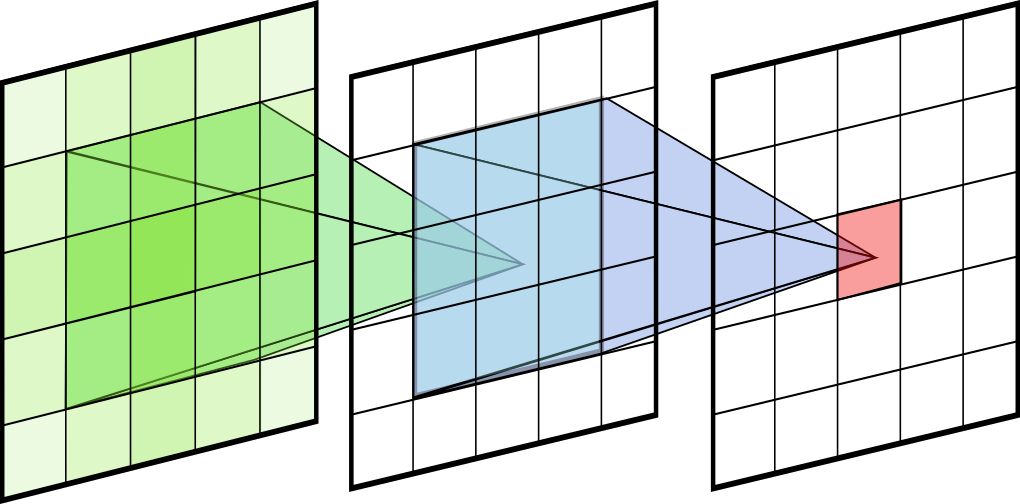
\includegraphics[width=0.5\textwidth]{revue_litterature/3by3equal5.png}
	\caption{Illustration de la notion de champs visuel réceptif obtenu par la mise en séquence de deux couches convolutives de masque $3 \times 3$. Pour obtenir la valeur du pixel rouge, il faut prendre les $3 \times 3$ pixels de l'image de la couche précédente, eux-même tous obtenus en utilisant les $5\times 5$ pixels de la couche d'entrée. On peut donc parler de champs visuel réceptif de $5 \times 5$ pour la troisième couche.}
	\label{fig:TheoricalReceptiveField}
\end{figure}
Notons cependant que la notion de champs visuel théorique ne correspond pas à une réelle mesure d'importance d'un pixel d'entrée de réseau vis-à-vis d'un pixel en sortie d'une des couches convolutives. Il s'agit plutôt d'une borne supérieure, en pratique jamais atteinte, sur le contexte spatial pris en compte dans l'estimation de la sortie d'une couche donnée. Luo et al. proposent une estimation probabiliste du champs visuel réceptif effectif \cite{luoUnderstandingEffectiveReceptive2016} faisant l'hypothèse d'une distribution Gaussienne des noyaux des masques convolutifs. Ils démontrent que le champs visuel réceptif effectif est en pratique bien inférieur à son estimation théorique.

\paragraph{Inception-V1}
Contemporain du VGG, Szegedy et al. proposent le GoogleNet, s'appuyant sur un nouveau type de module appelé \textit{Inception-block} \cite{szegedyGoingDeeperConvolutions2015a}. Les auteurs documentent également l'utilisation d'un certain nombre de techniques permettant de réduire le nombre de paramètres du réseau par couches (et donc d'augmenter le nombre de celles-ci). En particulier, leur architecture fait usage de convolution de taille $1 \times 1$. En apparence, une telle opération n'est qu'une combinaison linéaire des cartes de caractéristiques qui lui sont fournies. Elle permet cependant d'en réduire la dimension, à l'instar d'un opérateur de compression. De plus, l'ajout d'une fonction non-linéaire à la sortie de chacune des convolutions $1 \times 1$ permet la composition de fonctions de plus en plus complexes.
Quant à lui, le bloc \textit{Inception} (Figure \ref{fig:InceptionBlock}) a pour principale originalité la mise en parallèle de diverses couches convolutives, chacune ayant sa propre paramétrisation (différentes tailles de masque). Les caractéristiques extraites par chaque couche sont ensuite fusionnées via un opérateur dédié.

\begin{figure}[htb]
	\centering
	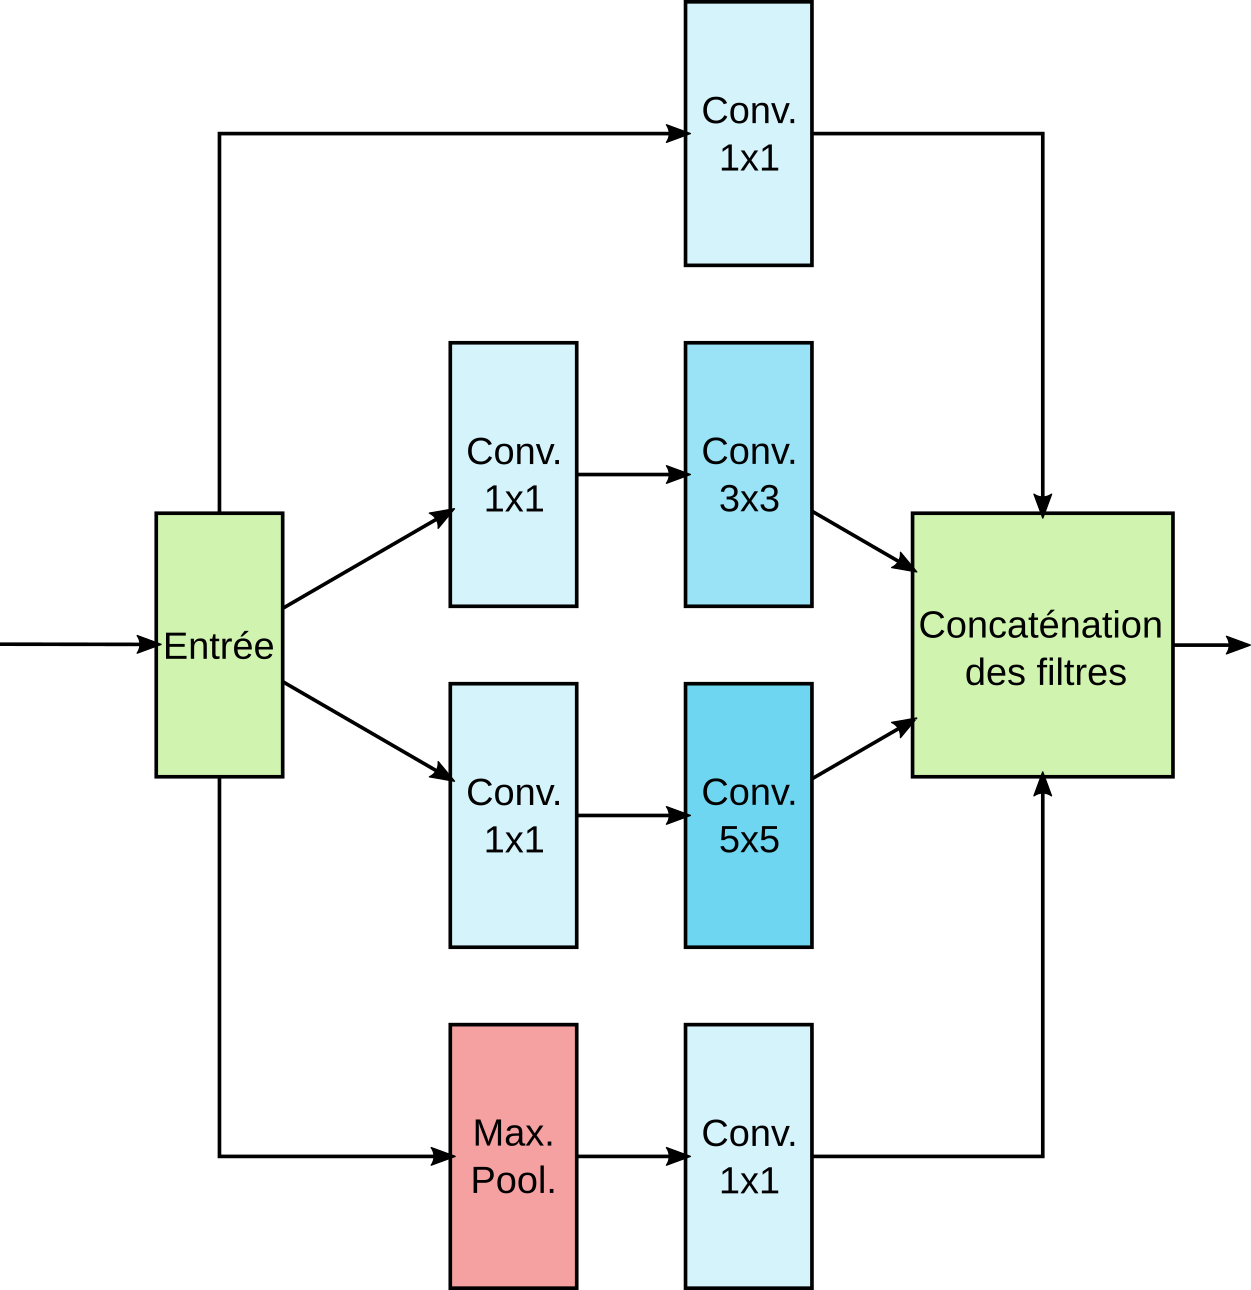
\includegraphics[width=.4\textwidth]{revue_litterature/module_inception}
	\caption{Illustration de l'\textit{Inception block} proposé par Szegedy et al. pour l'architecture GoogleNet \cite{szegedyGoingDeeperConvolutions2015a}}
	\label{fig:InceptionBlock}
\end{figure}

L'utilisation de ces voies parallèles oriente la recherche vers des réseaux de plus en plus profonds, c'est-à-dire constituée de séquences de couches toujours plus longues. Or, deux problèmes sont rapidement identifiés:
\begin{itemize}
	\item La composition de fonctions entraîne une évanescence (ou au contraire, une explosion) des gradients sur certaine couche lors de l'opération de rétro-propagation. Dans une certaine mesure, cet effet peut être contrôlé par une initialisation judicieuse des poids du modèle\cite{glorotUnderstandingDifficultyTraining2010, heDelvingDeepRectifiers2015} ou l'utilisation de couches de normalisations intermédiaires \cite{ioffeBatchNormalizationAccelerating2015, ulyanovInstanceNormalizationMissing2016a, baLayerNormalization2016}.
	\item Il a été observé qu'un réseau plus profond est sujet à une dégradation de ses performances \cite{heConvolutionalNeuralNetworks2015a, srivastavaHighwayNetworks2015}, non seulement sur l'ensemble de test, mais également sur celui d'apprentissage. Un tel effet est contre-intuitif: ajouter des poids ne devrait théoriquement pas dégrader les performances sur l'ensemble d'apprentissage. En effet, dans le pire des cas, le réseau pourrait se passer des couches supplémentaires en les mappant vers la fonction identité. Cette dégradation n'est donc pas la conséquence d'un sur-apprentissage lié à un excès de paramètres.
\end{itemize}
Ces observations ont motivé la recherche vers de nouvelles formes d'architectures telles les \textit{Highway Network} \cite{srivastavaHighwayNetworks2015} ou les \textit{Residual Network} \cite{heDeepResidualLearning2016b}. Toutes deux ont pour objectif d'accroître la profondeur du réseau (jusqu´à plus de cent couches convolutives) tout en résolvant les problèmes liés aux gradients. Nous détaillons ici la dernière; ses performances l'ayant rendu très populaire, la rendant aujourd'hui encore très utilisée.

\paragraph{Residual Network}
\label{sec:resnet}
He et al. introduisent la notion de connexions résiduelles pour augmenter significativement le nombre de couches du réseau \cite{heDeepResidualLearning2016b}. Le raisonnement des auteurs est le suivant: si un ensemble de couches non linéaires successives peut approximer n'importe quelle fonction $\mathcal{H}(x)$, il lui est tout autant possible d'approximer la fonction résiduelle $\mathcal{F}(x) = \mathcal{H}(x) - x$. La fonction originale se retrouve donc simplement par addition $\mathcal{F}(x) + x$, qui est au c\oe ur du \textit{ResNet}: l'entrée d'une (ou plusieurs) couche est additionnée à sa sortie, on parle alors de connexion résiduelle. Cette \og astuce \fg permet d'accroître la taille du réseau: en effet cette connexion facilite la propagation des gradients. Par ailleurs, toute section $\mathcal{F}(x)$ du réseau potentiellement inutile pourra converger vers la fonction nulle; la connexion résiduelle assurant que l'identité sera conservée. Les auteurs démontrent que ces connexions améliorent grandement les performances d'un réseau profond (jusqu'à 101 couches), tout en maintenant celle d'un réseau plus superficiel.

\begin{figure}[htb]
	\centering
	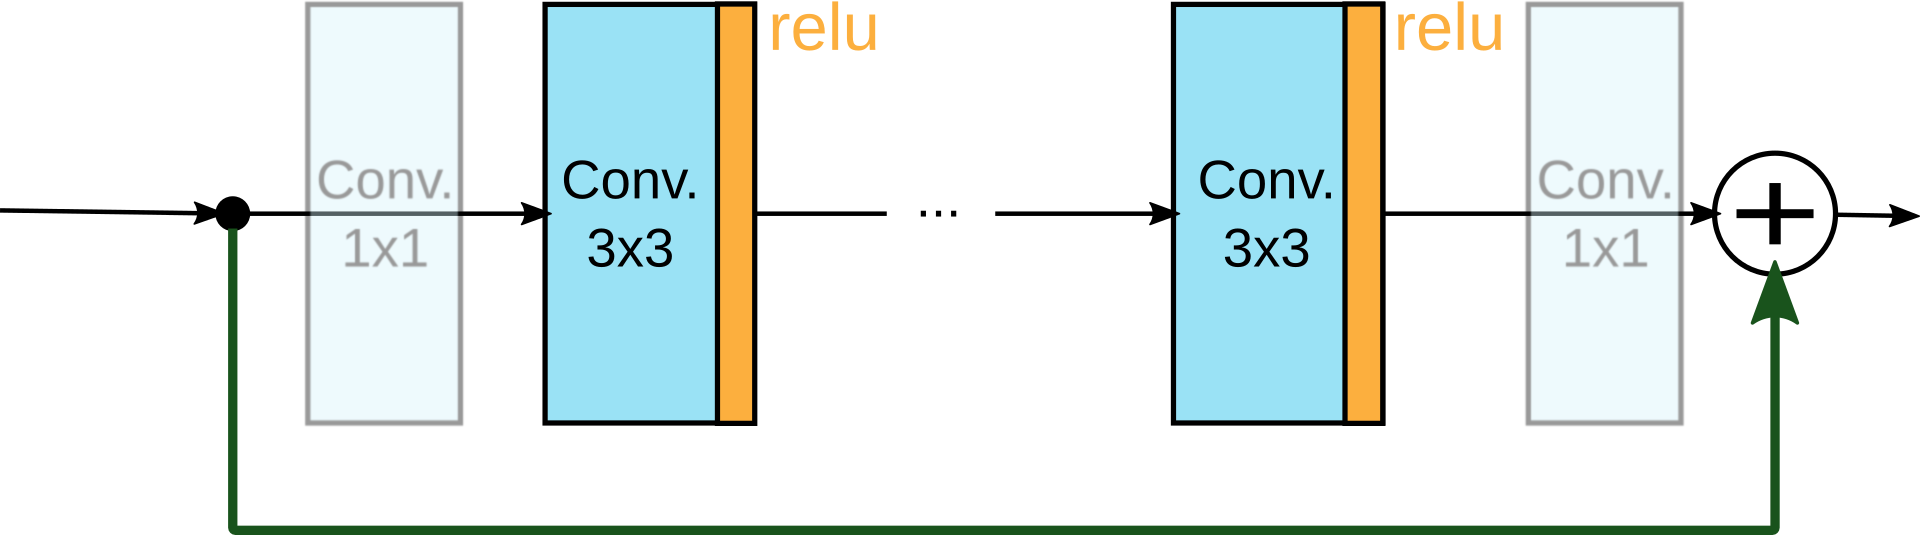
\includegraphics[width=.7\textwidth]{revue_litterature/residual_connection}
	\caption{Connexion résiduelle proposée par He et al. pour l'architecture ResNet \cite{heDeepResidualLearning2016b}. Les convolutions $1\times 1$ placées en entrée et sortie sont optionnelles: elles permettent la projection des cartes de caractéristiques vers des espaces aux dimensions concordantes si nécessaire.}
	\label{fig:ResNet}
\end{figure}

\paragraph{DenseNet}
Huang et al. étendent le concept des connexions résiduelles à travers une nouvelle architecture nommée DenseNet \cite{huangDenselyConnectedConvolutional2017}. À l'inverse du ResNet, pour lequel les connexions résiduelles sont arbitrairement choisies, le DenseNet s'appuie sur un principe de connexion complète: chaque sortie de couche est envoyée en entrée de toutes les couches suivantes appartenant a un même bloc, où chaque bloc est délimité par une opération de pooling. Autrement dit, toutes les couches au sein d'un même bloc possède la même résolution spatiale. Au sein d'un bloc de $L$ couches, il existera donc $\frac{L\cdot(L+1)}{2}$ connexions au lieu des $L+1$ du ResNet. Autre différence avec ce dernier, la connexion résiduelle ne se fait pas par une addition, mais avec une concaténation des cartes de caractéristiques. Pour limiter une sur-paramétrisation du modèle, chaque couche est limitée à douze cartes de sortie, ce qui est significativement plus petit que dans les précédents travaux décrits. Malgré cela, les auteurs obtiennent des performances supérieures à l'état de l'art et montrent que grâce à ces connexions \og denses\fg, le problème des gradients évanescents disparaît. Une des hypothèses fournies pour expliquer cette efficacité repose sur l'idée que la structure dense favorise la réutilisation des caractéristiques entre couches successives, ce qui va dans le sens d'un meilleur signal propagé.

\paragraph{SqueezeNet}
\label{par:squeezeNet}
Inspirés par les premiers modèles d'attention (\cite{wangResidualAttentionNetwork2017}), Hu et al. \cite{huSqueezeandExcitationNetworks2018} proposent une nouvelle architecture appelée SqueezeNet. Son originalité repose sur le module \textit{Squeeze-\&-Excite}. L'idée, là encore, est d'élargir le contexte spatial pris en compte dans une couche convolutive: en effet, le noyau de convolution basique n'a un effet que local, les relations contextuelles à plus large échelle sont donc ignorées. Jusqu'ici, cet effet a été corrigé en accumulant séquentiellement les couches convolutives, mais Hu et al. proposent une autre approche. L'idée est de construire, pour chaque couche, un vecteur contextuel encapsulant les relations globales. Celui-ci est obtenu par \textit{Global Mean Pooling} (c'est-à-dire la moyenne spatiale du tenseur des caractéristiques en sortie de couches), avant d'être fourni à un simple réseau \ac{PMC} à deux couches qui maintient les dimensions du vecteur. La première étape correspond au compression des caractéristiques (\textit{Squeeze}), la seconde à leur excitation. Le vecteur résultant est ensuite passé à travers une fonction sigmoïde $\sigma$ afin de borner ses valeurs dans l'intervalle $\left[ 0, 1\right]$. L'étape d'excitation consiste à multiplier ce vecteur au tenseur d'entrée, venant ainsi pondérer chacune des caractéristiques de celui-ci. Cette pondération est souvent associée à la notion d'attention, car elle permet de concentrer le réseau sur certaines cartes de caractéristiques précises. 

\subsection{Modèles de segmentation sémantique}
\label{sec:ModeleSegmentation}
Les modèles présentés dans la section précédente ont pour point commun de se limiter à la classification d'images. Autrement dit, pour une image, la sortie de ces réseaux aura la forme d'un vecteur indicateur de la classe prédite. Mais pour de nombreuses applications et tout particulièrement dans le domaine médical, il est souvent nécessaire d'obtenir une granularité plus fine et obtenir une classification à l'échelle du pixel plutôt que de l'image. Cette opération est appelée \textbf{segmentation sémantique}. Si les architectures présentées jusqu'ici ne sont pas initialement conçues pour cela, il est aisé de les adapter. Une façon de le faire est d'entraîner le modèle à prédire la classe d'appartenance d'un \textit{patch} (morceau) d'image; en recombinant chaque patch, on reconstruit une image segmentée. On retrouve dans l'idée cette approche dans les travaux précurseurs de Farabet et al. \cite{farabetLearningHierarchicalFeatures2013}. L'inconvénient de cette approche est de limiter la prise en compte du contexte à la taille du patch considéré. Farabet et al. résolvent ce problème par l'utilisation des \ac{CRF}, méthode qui suit la théorie statistique des Champs de Markov et qui regroupe les pixels présentant une apparence similaire à travers l'image conditionnellement à une pré-segmentation. Il s'agit donc d'une étape de post-traitement qui a pour avantage de prendre en compte le contexte global de l'image. Le second inconvénient du modèle de Farabet et al. est de produire une  segmentation dont la résolution est tributaire de la taille du patch choisi: plus celui-ci est grand, plus la résolution sera faible. Mais inversement, pour des petits patches, segmenter toute l'image prendra un temps considérablement plus long. \\
Ces deux inconvénients ont poussé au développement d'un nouveau type d'architecture de réseau de neurones que nous présentons ici.
\subsubsection{Réseau entièrement convolutif}
\label{sec:FCCN}


Long et al. \cite{longFullyConvolutionalNetworks2015a} seront les premiers à se passer d'une couche de classification dans leurs travaux sur la segmentation. Plutôt que de reprendre la structure conventionnelle: $N \times (\text{Couches convolutives} \rightarrow \text{Pooling}) \rightarrow K \times \text{Couches totalement connectées} \rightarrow \text{Classification}$ (qui décrit plus ou moins toutes les architectures de la section précédente), les auteurs suggèrent de ne garder que la première étape (les $N$ couches convolutives), afin de conserver la structure spatiale des cartes de caractéristiques que le pooling détruit. Chacun des pixels appartenant à ces cartes est ensuite projeté vers sa classe prédite. Ce faisant, au lieu de passer d'une fonction de coût par image, on obtient une fonction de coût par pixels. La spécificité de cette architecture est donc de n'utiliser que des couches convolutives et de ré-échantillonnage (pooling, unpooling ou interpolation). En revanche, dans les travaux de Long et al. la prédiction finale reste raffinée par l'utilisation des \ac{CRF}. L'opération de ré-échantillonnage permet d'interpoler les cartes de caractéristiques vers la résolution initiale de l'image d'entrée. Cette opération peut se faire aussi bien par simple interpolation bilinéaire que par déconvolution.
\paragraph{DeepLab-V3}
L'architecture DeepLab-V3, introduite en 2017 par Chen et al. \cite{chenRethinkingAtrousConvolution2017} franchit un palier technologique, en obtenant de hautes performances malgré l'absence d'utilisation d'un post-traitement de type \ac{CRF}. Comme son nom l'indique, il s'agit de la troisième itération d'une architecture dont chaque composant a été soigneusement testé. Elle se caractérise par l'utilisation de blocs basés sur l'idée des connexions résiduelles de type ResNet (paragraphe \ref{sec:resnet}) et surtout l'introduction du module ASPP (pour \textit{Atrous Spatial Pyramid Pooling}). La notion de convolutions atrous (à trous) est fondamentale pour cette architecture, en cela qu'elle permet, à moindre frais, la prise en compte d'un plus grand contexte spatial et sans ajouter de paramètres au modèle. Son mécanisme est illustré sur la figure \ref{fig:aTrousConvolutions}.

\begin{figure}[!h]
	\centering
	\begin{subfigure}[t]{0.48\textwidth}
	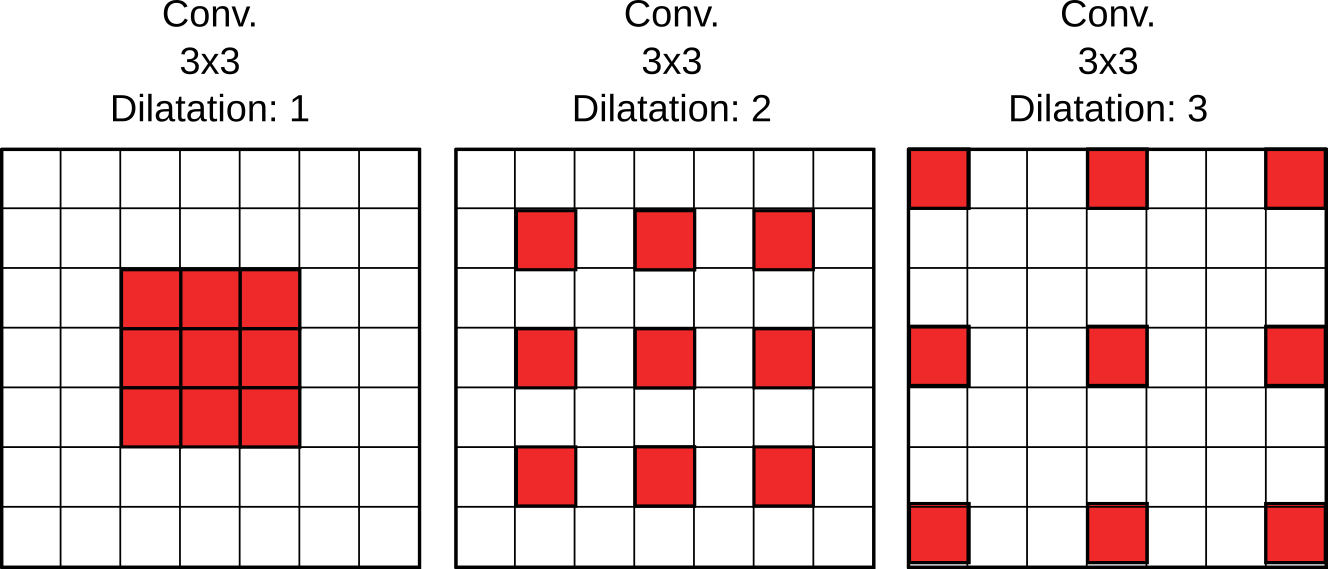
\includegraphics[width=\textwidth]{revue_litterature/convolutions_a_trous.png}
	\caption{Principe illustrée de la convolution à trous (ou dilatées). Pour un même nombre de paramètres (ici $3 \times 3$), le champs réceptif est artificiellement accru en les espaçant.}
	\end{subfigure}
	\hfill
	\begin{subfigure}[!ht]{0.45\textwidth}
		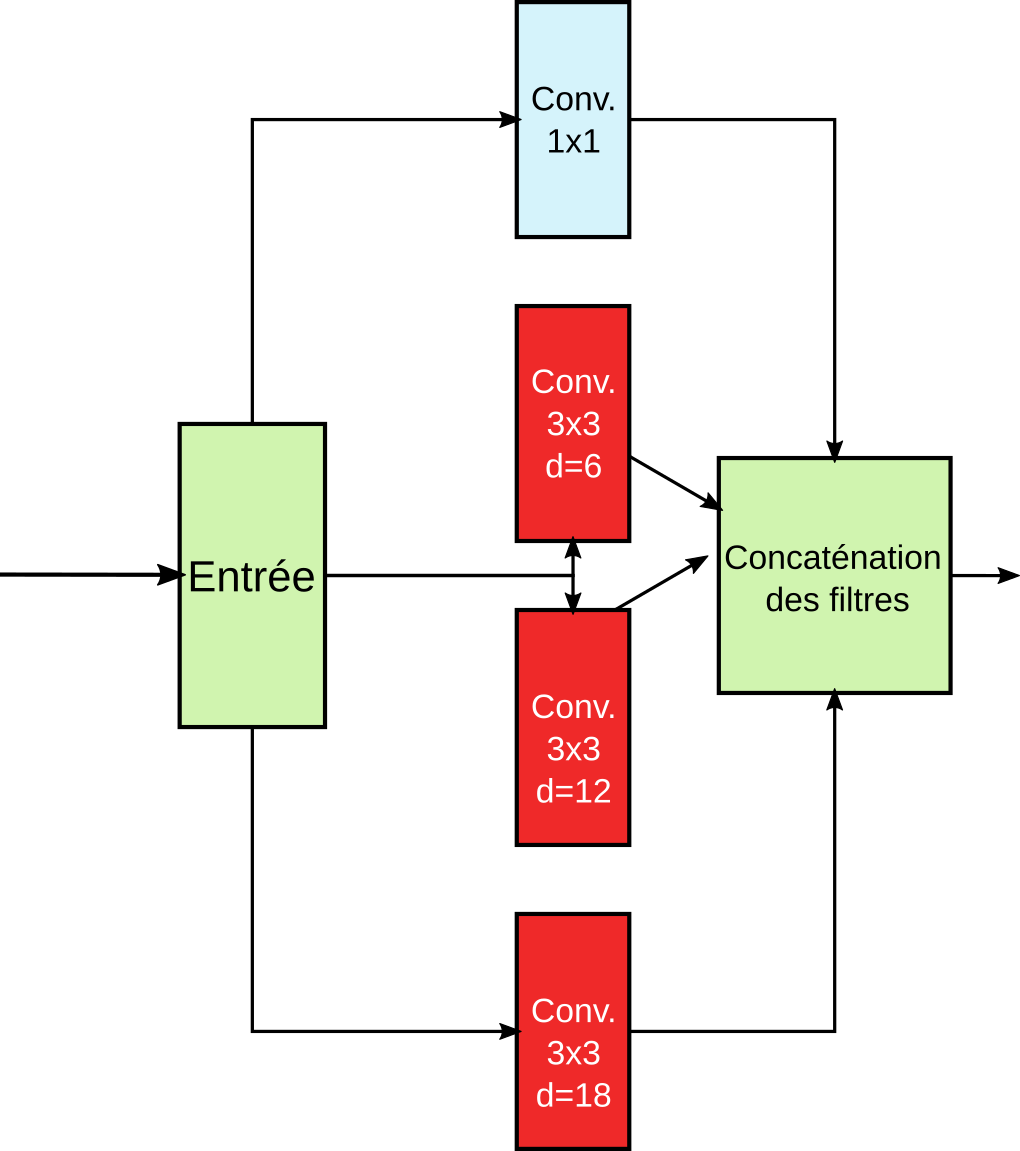
\includegraphics[width=\textwidth]{revue_litterature/ASPP}
		\caption{Module ASPP. La variable $d$ indique les différents coefficients de dilatation.}
	\end{subfigure}

	\caption{Illustrations des modules utilisées dans l'architecture DeepLabV3\cite{chenRethinkingAtrousConvolution2017}}
	\label{fig:aTrousConvolutions}
\end{figure}

\paragraph{U-Net}
\label{par:Unet}

Introduite par Ronneberger et al. \cite{ronnebergerUNetConvolutionalNetworks2015b}, l'architecture U-Net est certainement une des plus emblématiques en ce qui concerne la segmentation sémantique d'image médicale, du moins la plus citée. Outre sa simplicité, un de ses plus gros atouts est sa capacité à générer d'excellentes performances même en disposant que de peu de données d'entraînement. Une représentation de l'architecture est fournie sur la figure \ref{fig:UnetArchitecture}. Sa structure respecte le principe, souvent repris depuis, d'encodeur/décodeur. L'encodeur fonctionne similairement à la plupart des architectures présentées jusqu'ici, c'est-à-dire en compressant progressivement les dimensions spatiales de l'image tout en enrichissant le vecteur descriptif à chaque pixel de nouvelles composantes. Le décodeur pour sa part fait l'exact inverse et ré-interpole progressivement les cartes de caractéristiques jusqu'à la dimension de l'image. Cependant, le U-Net se distingue de ce simple principe en ajoutant des connexions passerelles entre chaque étape de l'encodeur et du décodeur. Celles-ci ont deux objectifs:
\begin{itemize}
	\item Maintenir la propagation des gradients intacte malgré le nombre de couches du réseau, similairement à ce que fait le ResNet.
	\item Affiner les détails de segmentation des petites structures. En effet, du fait du principe de sous-échantillonnage/ré-interpolation, les réseaux de segmentation ont tendance à effacer les plus petites structures. En ajoutant ces connexions passerelles, le U-Net corrige cet effet.
\end{itemize}
\begin{figure}[!htb]
	\centering
	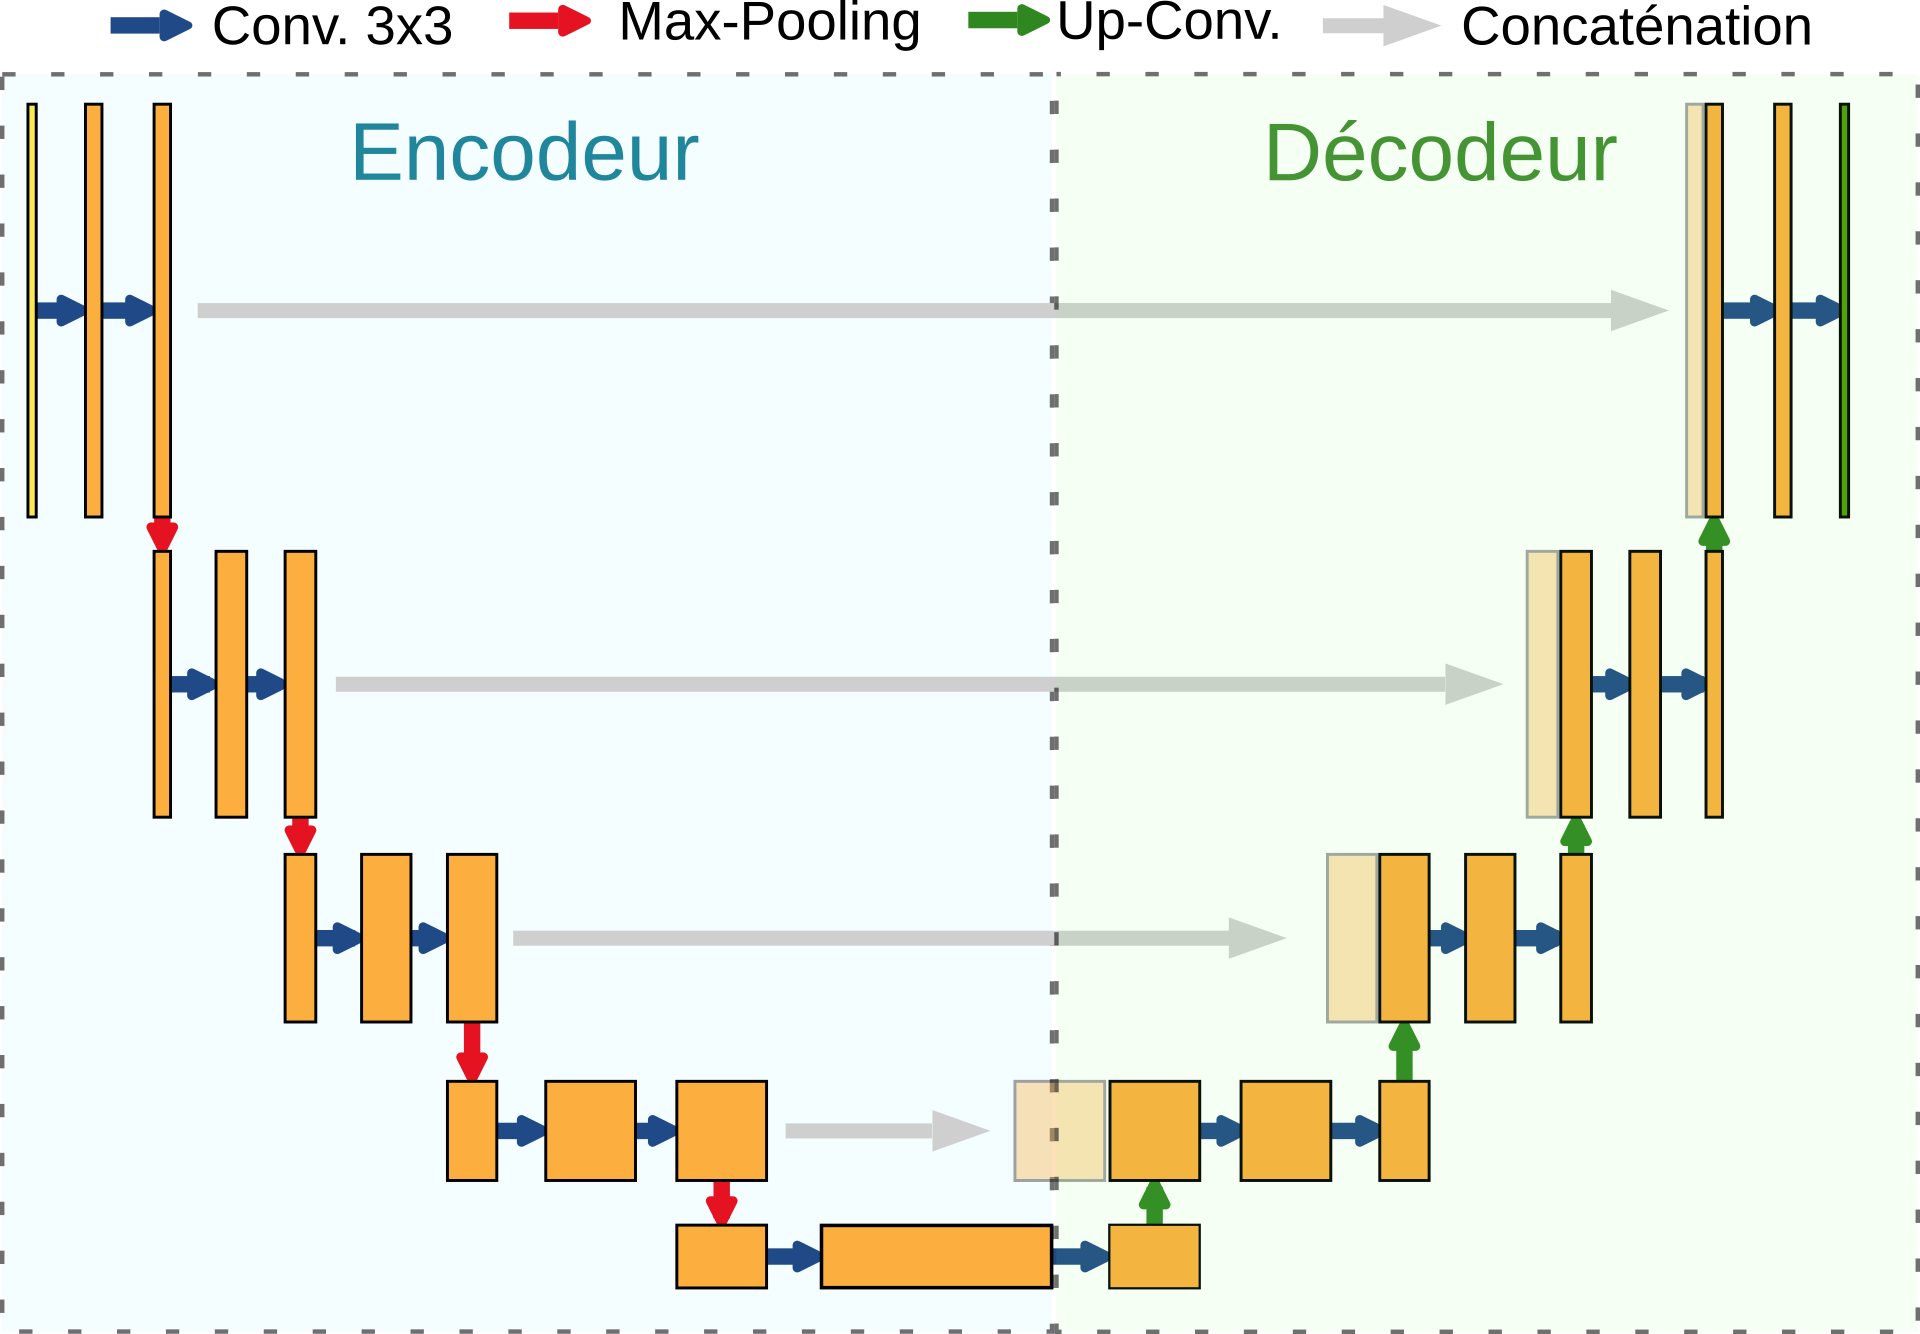
\includegraphics[width=.7\textwidth]{revue_litterature/unet}
	\caption{Architecture originale du U-Net}
	\label{fig:UnetArchitecture}
\end{figure}
\paragraph{Variantes du U-Net}
L'architecture du U-Net est fondatrice pour sa structure en \og U\fg basé sur un couple encodeur/décodeur symétrique. Peut-être en raison de sa facilité d'implémentation, ce concept a inspiré une pléthore de variantes. Bien souvent, les améliorations proposées s'appuient sur des modules empruntés à d'autres architectures pré-existantes. Par exemple, Rundo et al. \cite{rundoUSENetIncorporatingSqueezeandExcitation2019} créent le SE-U-Net en incorporant le module Squeeze-\&-Excite dans les différentes couches d'encodeur et décodeur pour la segmentation d'image d'IRM, Oktay et al. \cite{oktayAttentionUNetLearning2022} ajoutent un mécanisme d'attention sur une variante du U-Net adaptée aux images tridimensionnelles dédiée à la segmentation du pancréas, Zhou et al. \cite{zhouUNetRedesigningSkip2020} étendent le concept des connexions denses (de type \textit{DenseNet}) entre les couches d'encodage et décodage de leur réseau appelé U-Net++. 
\\
Il ne s'agit là que de quelques exemples parmi de nombreux autres, qui témoignent parfaitement de la modularité des architectures de réseaux de neurones. 

\newpage

\subsection{Optimisation et entraînement de modèles}
Malgré la diversité des architectures, il est remarquable que celles-ci adoptent essentiellement la même stratégie pour ajuster leurs paramètres lors de la phase d'entraînement. Cette section a pour objectif de clarifier ce mécanisme de manière formelle pour s'accorder sur une définition de l'apprentissage. Précisons que nous nous limitons ici au problème de l'apprentissage supervisé (autrement dit, pour lequel il existe une référence explicite à atteindre, appelée vérité terrain). Bien souvent le cas de l'apprentissage non-supervisé aborde l'entraînement de manière similaire, avec cependant une reformulation de l'objectif visé. \\
Dans un cas comme dans l'autre, l'entraînement utilise un jeu de données, en pratique souvent de taille conséquente, pour mettre à jour les paramètres du modèle de manière itérative. Ce processus s'arrête une fois la convergence atteinte vers un modèle jugé satisfaisant. Nous le détaillons ici.\\

Soit un jeu de données $\mathcal{S} = \{ (x_m, y_m) \in \mathbb{R}^d \times \{1, ...,K\}^{d'}\}, |S|=M$, c'est à dire $M$ échantillons ($x_m$ de dimension $d$), chacun venant avec une classe associée représentée par le label $y_m$ prenant valeur parmi les $K$ classes possibles. La dimension $d'$ du vecteur de label dépend de l'application considérée: ainsi pour la classification d'images, en général $d'=1$ (une seule classe par image), pour la segmentation sémantique, $d'=d=H\times W$ où $H, W$ représentent la hauteur et la largeur de l'image (une classe par pixel de l'image). \\
Le réseau de neurones que l'on souhaite entraîner est représenté sous la forme d'une fonction $f_\theta: \mathbb{R}^d \to  \{1, ...,K\}^{d'}$, où $\theta$ englobe tous les paramètres (ou poids) du modèle. 
Cette configuration représente le cas typique rencontré pour l'apprentissage supervisé d'un modèle multiclasse (y compris pour de la segmentation).
Un modèle $f_{\theta^\star}$ idéalement entraîné sur les données $\mathcal{S}$ saura faire une association parfaite entre $x_m$ et sa classe associée par la vérité terrain\footnote{Il s'agit d'une simplification volontaire, car la sortie d'un réseau de neurones est continue et non discrète. En réalité, on modélise plutôt la sortie réseau comme une estimation de la probabilité d'appartenance à chaque classe.}, c'est-à-dire : 
\begin{equation}
	f_{\theta^\star}(x_m) = y_m, \forall\, 1 \leq m \leq M
\end{equation} 
En revanche, un modèle non-idéal commettra des erreurs. On les quantifie par une fonction de coût (ou d'erreur) notée $\mathcal{L}(f_\theta(x_m), y_m)$ évaluée pour chaque point de $\mathcal{S}$. En la calculant sur l'ensemble des données, on obtient une fonction de coût global:
\begin{equation}
	J(\theta) = \sum_{m=1}^{M} \mathcal{L}(f_\theta(x_m), y_m)
\end{equation}
Seule la dépendance à $\theta$ est indiquée dans la fonction d'erreur $J$, car il s'agit de la seule variable d'intérêt à optimiser. 
À titre d'exemple, la fonction d'erreur au carré moyenne (connue sous le nom de \ac{MSE}) mesure directement l'écart entre la sortie du modèle et le label associé à son entrée\footnote{Le carré garantit la positivité de la fonction}:
\begin{equation}
	J(\theta) = \frac{1}{M}\sum_{m=1}^{M}(f_\theta(x_m) - y_m)^2
\end{equation}
En construisant ainsi une fonction de coût, on peut définir la notion d'entraînement de manière formelle: il s'agit de trouver les paramètres $\theta^\star$ qui minimiseront $J(\theta)$, c'est à dire qui diminueront l'erreur globale sur l'ensemble des données à disposition:
\begin{equation}
	\theta^\star = \argmin_{\theta} J(\theta)
\end{equation}
Le problème de cette minimisation se ramène à un calcul d'optimisation numérique que nous détaillons au prochain paragraphe. Mais ouvrons une courte parenthèse pour préciser qu'il s'agit d'une vision tronquée de l'apprentissage machine, qui en réalité s'appuie sur la théorie de l'apprentissage statistique et justifie l'entraînement d'un réseau comme une tentative de modélisation de la distribution de probabilités décrivant $\mathcal{S}$.
Cette interprétation probabiliste sera détaillée à la fin de cette section, mais nous fermons pour l'instant cette parenthèse pour revenir à la notion d'optimisation.
\subsubsection{Descente de gradients}
Abstraction faite de la théorie justifiant cette approche, l'entraînement d'un réseau de neurones se résume à un problème d'optimisation numérique d'une fonction d'erreur. Deux types de solutions existent pour un tel problème:
\begin{enumerate}
	\item Une solution unique $\theta^\star$ telle que $J(\theta^\star) \leq J(\theta), \forall \theta$ est qualifiée de minimum global.
	\item Si la solution identifiée n'est valable que dans un voisinage $\mathcal{N}$ de $\theta^\star$, c'est à dire $J(\theta^\star) \leq J(\theta), \forall \theta \in \mathcal{N}$, on parle alors de minimum local.
\end{enumerate}
Notons que si la fonction à optimiser $J$ est convexe, les minimum local et global se confondent. Une grande partie de la recherche en optimisation se concentre donc sur les problèmes convexes; mais il est bien connu que les réseaux de neurones n'appartiennent pas à cette catégorie.
Idéalement, l'entraînement devrait aboutir à une solution $\theta^\star$ globale: elle indiquerait ainsi la meilleure configuration de paramètres du modèle parmi l'ensemble des possibilités. En pratique, il est quasiment impossible d'identifier un minimum global et on se contente d'en rechercher un local (il peut y en avoir naturellement plus d'un). Il est aisé de reconnaître un minimum local en faisant quelques hypothèses faibles: il est nécessaire que la fonction de coût global, $J(\theta): \mathbb{R}^N \to \mathbb{R}$ soit différentiable presque partout (où $N$ est le nombre de paramètres du modèle). Tout minimum, local ou global, vérifie alors:
\begin{equation}
	\label{eq:OptimalPointTheta}
	\nabla J(\theta^\star) = 0
\end{equation}
La démonstration de ce résultat est une application quasi-directe du théorème de Taylor. L'équation \ref{eq:OptimalPointTheta} permet de définir un critère d'arrêt de l'entraînement, correspondant à la découverte d'un minimum local. Partant d'une initialisation $\theta_0$ du modèle, il reste alors à trouver le chemin menant à $\theta^\star$ (ou du moins une valeur approchée). Pour y arriver, tous les algorithmes d'optimisation génèrent une séquence $\{\theta_k\}_{k=0}^{\infty}$ et définissent des règles d'évolution. Il existe deux grandes stratégies pour trouver ces itérations. La première a trait à la recherche de ligne directrice (direction à prendre dans l'évalution des $\theta_k$) tandis que la seconde transforme le problème en la recherche d'une région de confiance (dans l'espace des paramètres); toutes deux ont fait l'objet d'importantes recherches ces cinquante dernières années largement documentées par Nocedal J. et Wright S. \cite{nocedalIntroduction2006}. 
\\
L'entraînement d'un réseau de neurone appartient à la première catégorie. À chaque itération $k$, la fonction de coût est évaluée au point $\theta_k$. On choisit ensuite une direction $p_k \in \mathbb{R}^N$ qui permet de décroître la fonction de coût et on se déplace le long de celle-ci sur une certaine longueur $\alpha_k \in \mathbb{R}^+$ avec pour objectif de remplir ces deux conditions:
\begin{equation}
	 \left\{ \begin{array}{cl}
		\theta_{k+1} &= \theta_k + \alpha_k p_k \\
		J(\theta_{k+1}) &\leq J(\theta_{k})
	\end{array} \right.
\end{equation}
Dans le contexte de l'entraînement d'un réseau de neurones, le scalaire $\alpha_k$ porte le nom de \textit{pas d'apprentissage}. 
\\
Toujours en s'appuyant sur la décomposition de Taylor de la fonction de coût, on peut montrer que la direction de plus forte diminution suit le gradient au point $\theta_{k}$. Dans le cadre de l'entraînement, on choisit donc généralement:
\begin{equation}
	p_k = -\nabla J(\theta_k)
\end{equation}
d'où l'appellation \og descente de gradients\fg tire son nom. Notons qu'il ne s'agit pas forcément de la direction optimale pour atteindre le minimum; uniquement la direction de plus forte descente au point considéré. La méthode de Newton suggère par exemple de calculer la direction:
\begin{equation}
	p_k = - \nabla^2 J_k ^{-1} \nabla J_k
\end{equation}
Qui fait intervenir la Hessienne inversée de la fonction $J$ au point $\theta_{k}$. Malheureusement, ni le calcul de dérivées d'ordre supérieur à 1 (pour la Hessienne), ni le calcul de son inverse ne sont en pratique réalisables pour un réseau de neurones. En effet, rappelons que $J$ a pour support $\mathbb{R}^N$, où $N$ représente le nombre de paramètres du modèle. Celui-ci peut se compter en milliers (voire bien plus pour les plus gros modèles). Cette complexité rend inutilisable une grande partie des techniques développées en optimisation numérique dès lors qu'il s'agit d'une architecture un tant soit peu conséquente.
De la même manière, il existe une abondante littérature sur le choix optimal du pas d'apprentissage en fonction de la direction choisie \cite{nocedalLineSearchMethods2006}, mais en pratique, l'entraînement d'un réseau de neurones utilise des heuristiques bien plus simples.

\subsubsection{Descente de gradients stochastique}
En choisissant $p_k = -\nabla J(\theta_k)$, l'algorithme de descente de gradients peut se réécrire:
\begin{align}
	\theta_{k+1} &= \theta_{k} - \alpha_k \nabla J(\theta_k) \\
	&= \theta_{k} - \alpha_k \nabla \sum_{m=1}^{M} \mathcal{L}(f_{\theta_k}(x_m), y_m)
\end{align}
Sous cette forme, il apparaît clairement que le calcul de l'estimateur $J(\theta_k)$ fait intervenir l'ensemble des données pour le calcul des contributions individuelles $\mathcal{L}$, et ce pour chaque itération $k$ d'apprentissage. Dans la pratique, où les données $\mathcal{S}$ peuvent contenir plusieurs milliers ou millions de points, il est bien souvent très inefficace (voire impossible) de calculer le gradient global. On peut en revanche en calculer une estimation. Pour cela, on définit la famille de parties $\{\mathcal{B}_i \subset \mathcal{S} | \bigcup_i \mathcal{B}_i = \mathcal{S} \} $ de telle sorte que chaque élément de $\mathcal{B}_i$ est tiré sans remise aléatoirement de $\mathcal{S}$. L'algorithme se base ainsi sur une estimation du gradient global sur un sous-ensemble de données:
\begin{equation}
	\theta_{k+1} = \theta_{k} - \alpha_k \nabla \sum_{m \in \mathcal{B}_i}\mathcal{L}(f_{\theta_k}(x_m), y_m)
\end{equation} 
À chaque itération $k$, un nouveau sous-ensemble $\mathcal{B}_i$ \footnote{Appelé \textit{mini-batch} en anglais} est choisi, correspondant donc à un échantillonnage aléatoire des données d'entraînement. On parle donc de descente de gradients stochastiques. Dépendamment d'hypothèses plus ou moins fortes, il est possible de démontrer la convergence uniforme d'un tel processus itératif. Mais nous nous contenterons ici de cette description sommaire, suffisante pour introduire une technique qui appartient en réalité au vaste domaine des algorithmes stochastiques et des martingales, pour lequel il existe de nombreux résultats théoriques fondamentaux \cite{godichon-baggioniAlgorithmesStochastiques}. Néanmoins, la version simple présentée ici est bien celle employée pour l'apprentissage des réseaux de neurones.
\subsubsection{Propagation inverse des gradients}
Jusqu'ici, nous avons présenté la manière de minimiser une fonction de coût à partir de la mise à jour de ses variables par descente de gradient (stochastique ou non). Mais nous avons passé sous couvert la manière dont sont calculés ces gradients pour chacun des paramètres du modèle. Cela implique en particulier de rappeler la dépendance de la fonction de coût à ces paramètres. Remémorons-nous qu'un réseau de neurone $f_\theta: \mathbb{R}^d \to \{0,1,...,K\}^{d'}$ est une suite d'opérations appliquées à un vecteur d'entrée $\mathbf{x}$ pour produire une sortie $y$. Chacune de ces opérations implique son propre jeu de paramètres (d'où l'appellation de fonction paramétrique). Par exemple, une couche totalement connectée a pour paramètres un poids $\mathbf{W} \in \mathbb{R}^{\text{in} \times \text{out}}$ et un biais $\mathbf{B} \in \mathbb{R}^{\text{out}}$. Un réseau composé de $N$ couches totalement connectées $g_n$ peut donc s'écrire (on omet le biais par simplicité):
\begin{equation}
	\label{eq:simpleFeedForward}
	f(\mathbf{x}) = g^N(g^{N-1}(...g^1(\mathbf{x}, \mathbf{W}_{1}), \mathbf{W}_{N-1}), \mathbf{W}_N) = g_{\mathbf{W}_N}^N \circ g_{\mathbf{W}_{N-1}}^{N-1} \circ ... \circ g_{\mathbf{W}_1}^1 (\mathbf{x})
\end{equation}
Cette représentation du réseau sous la forme d'une composition de fonction est essentielle pour comprendre l'entraînement par rétro-propagation des gradients qui est au cœur de la méthode de mise à jour des poids. Donnons-nous comme outils pour cela le théorème de la dérivation des fonctions composées.
Soient $f, g$ deux fonctions à valeur dans $\mathbb{R}$ dérivables sur leur ensemble de définition respectif. Alors on a:
\begin{align}
	(g\circ f)' &= (g' \circ f) \times f' \\
	\Leftrightarrow \frac{d g \circ f}{dx} &= \frac{dg}{df}\frac{df}{dx} 
\end{align}
Ce théorème se généralise au-delà des fonctions scalaires. Soient $f: \mathbb{R}^n \mapsto \mathbb{R}^m$, $g:\mathbb{R}^m \mapsto \mathbb{R}$ et $h: \mathbf{X} \mapsto (g \circ f)(\mathbf{x})$. Alors on a:
\begin{align}
	\label{eq:GradientRuleComposition}
	\frac{\partial h}{\partial x_i} &= \sum_j \frac{\partial h}{\partial g_j}\frac{\partial f_j}{\partial x_i} \\
	\Leftrightarrow \nabla_{\mathbf{x}} h &= \left(\frac{\partial f}{\partial \mathbf{x}}\right)^T \nabla_{g} h
\end{align}
$\frac{\partial f}{\partial \mathbf{x}}$ est la matrice Jacobienne de $f$ de taille $n \times m$.
Or, en représentant un réseau de neurones en composition de fonctions (ses couches), l'application de ce théorème permet de calculer le gradient de chacun de ses paramètres. Qui plus est, une récursivité apparaît naturellement: en effet, l'équation \ref{eq:GradientRuleComposition} sépare le gradient en deux composantes multipliées entre elles:
\begin{enumerate}
	\item La Jacobienne $\frac{\partial f}{\partial \mathbf{x}}$, qui correspond intuitivement au calcul du gradient de l'opération réalisée à la couche considérée par rapport à son entrée.
	\item Le gradient $\nabla_{g} h$ de la couche suivante.
\end{enumerate}
En poursuivant le raisonnement, le gradient $\nabla_{g} h$ s'obtient à son tour par le produit de la Jacobienne de $g$ et du gradient de la fonction qui le suit, etc... Autrement dit, pour le calcul du gradient de la couche $n$, on utilisera le gradient calculé à la couche $n+1$. L'apparition d'un tel schéma récursif permet de grandement optimiser l'opération du calcul de gradients d'un réseau de neurones. En pratique, pour obtenir cette \textit{rétropropagation} des gradients, l'ensemble des opérations qu'il réalise est traduite sous la forme d'un graphe dirigé, où chaque variable issue d'une opération est représentée par un n\oe ud associé à cette opération. Les arêtes pointant vers un n\oe ud représentent les variables utilisées par l'opération du n\oe ud. Cette représentation, outre qu'elle permet un grand nombre d'optimisation (éliminer les n\oe uds inutiles, ceux qui ne sont pas pris en compte dans le calcul du gradient, etc.) établit un ordonnancement des opérations, depuis le vecteur d'entrée (par exemple une image), jusqu'à la valeur de sortie (en général, le coût associé).  $\mathcal{L}$ représente donc le dernier n\oe ud du graphe de compositions du réseau. En notant que naturellement, $\frac{\partial \mathcal{L}}{\partial \mathcal{L}} = 1$, on peut calculer le gradient de tous ses ancêtres en utilisant le théorème de la dérivation des fonctions composées, puis récursivement, des ancêtres des ancêtres, etc. Le grand intérêt de cette approche est la ré-utilisabilité des gradients de la couche $n+1$ pour calculer ceux de la couche $n$.

\subsubsection{Interprétation statistique}
\label{sec:interpretationProbabiliste}
Nous l'avons mentionné plus tôt lors de l'introduction de la notion de fonction de coût, l'apprentissage d'un réseau de neurones (et en réalité, l'essentiel des algorithmes d'apprentissage machine) peut s'interpréter sous le prisme du formalisme probabiliste, qui lui vient à la fois de sa capacité à établir une mesure (au sens mathématique) sur un ensemble et à l'inhérente stochasticité des données réelles utilisé à l'apprentissage. Nous couvrons dans cette section quelques éléments sommaires établissant les bases de ce formalisme. \\
On fait l'hypothèse que pour un jeu de donnée de $n$ éléments $\mathbb{X} = \{\mathbf{x}^{(1)}, ..., \mathbf{x}^{(n)}\}$, il existe une unique distribution (non accessible et inconnue) $p_{données}(\mathbf{x})$ d'où ont été tirés les échantillons de manière indépendante et identiquement distribuée. Le modèle, lui, prédit une probabilité par échantillons $f(\mathbf{x}, \theta)$
L'entraînement consiste alors à trouver le point $\theta^{\star} \in \Theta$ permettant d'estimer au mieux la vraie distribution des données (on parle d'estimateur statistique). \\
Pour cela, on introduit la notion de vraisemblance du modèle, définie par:
\begin{equation}
	\label{eq:maximumVraisemblance}
	L_n(\theta) = \prod_{i=1}^{n}f(\mathbf{x}^{(i)}, \theta)
\end{equation}
Elle correspond à la probabilité d'observation jointe de l'ensemble des variables $\mathbf{x}^{(i)}$ sous l'hypothèse qu'elles soient bien indépendantes et identiquement distribuées (I.I.D).
On souhaite trouver un modèle capable de maximiser cette probabilité étant données les variables dont nous disposons (qui sont donc bien observées).
L'articulation avec la notion de fonction de coût en découle directement: l'apprentissage est la recherche de l'estimateur de maximum de vraisemblance, c'est à dire:
\begin{equation}
	\theta^{\star}_n = \argmax_{\theta \in \Theta} L_n(\theta)
\end{equation}
Cette équation se ramène à la minimisation d'une fonction en prenant simplement l'opposé du maximum de vraisemblance. Notons qu'en pratique, plutôt que de manipuler le produit des probabilités, on préfère le substituer par une somme de logarithmes pour des raisons de stabilité numérique:
\begin{equation}
	 \argmax_{\theta \in \Theta} L_n(\theta) = \argmax_{\theta \in \Theta} \sum_{i=1}^{n}\log(f(\mathbf{x}^{(i)}, \theta)) = \argmin_{\theta \in \Theta} - \sum_{i=1}^{n}\log(f(\mathbf{x}^{(i)}, \theta))
\end{equation}
On peut facilement étendre l'équation au cas de l'apprentissage supervisé, pour lequel chaque échantillon $\mathbf{x}$ est accompagné d'un label représentant sa classe. Auquel cas, on souhaite que le modèle représente la distribution de probabilité dans l'espace des classes disponibles conditionnée à l'entrée observée. Autrement dit,
\begin{equation}
	f(\mathbf{x}^{(i)}, \theta) = p(\mathbf{y} | \mathbf{x}^{(i)})
\end{equation}
On définit alors, comme dans l'équation \ref{eq:maximumVraisemblance}, la vraisemblance-conditionnelle et on ramène le problème de l'apprentissage à sa maximisation:
\begin{equation}
	\theta^\star= \argmax_{\theta \in \Theta} \sum_{i=1}^{n} \log P(\mathbf{y}^{(i)}|\mathbf{x}^{(i)}; \theta)
\end{equation}

\section{Éléments de la théorie de l'apprentissage statistique}
\label{sec:theorieApprentissage}
Tout au long des expériences qui seront présentées dans les prochains chapitres, la notion de généralisation a occupé une place prédominante dans les questionnements de recherche. Elle a, selon les auteurs, une définition plus ou moins précise mais peut se résumer de la manière suivante: il s'agit de la capacité d'un modèle a maintenir de bonnes performances sur des données qu'il n'a jamais vu auparavant. Cette notion sera particulièrement discutée dans le chapitre \ref{sec:ChapitreSegmentation}, sous un angle empirique et appliqué aux données médicales qui nous intéressent. Mais il s'agit d'une notion fondamentale lorsqu'on parle de modélisation par apprentissage machine et elle occupe de fait une place aux premières loges des recherches théoriques sur l'apprentissage statistique. La difficulté à justifier les performances pratiques des réseaux de neurone a stimulé la curiosité des mathématiciens qui s'y intéressent et en fait un champs de recherche actif faisant appel à des concepts probabilistes avancés. Cette section n'a pas pour l'ambition de rentrer dans ces détails, mais d'en présenter le contexte dans un cadre définissant les notions de généralisation, de complexité, de capacité... \\
Nos propres travaux manipulent ces notions, mais sous un angle expérimental appliqué au domaine médical.
\subsection{Généralisation, sous-apprentissage et sur-apprentissage}
Pour reprendre la définition de Goodfellow et al. \cite{Goodfellow-et-al-2016}, le concept de généralisation d'un modèle est ce qui distingue l'apprentissage d'un \og simple \fg problème d'optimisation numérique. La généralisation traduit la capacité d'un modèle à maintenir ses propriétés sur des données qui n'ont pas servi à l'entraînement. Elle se mesure donc sur un ensemble disjoint de données, appelé ensemble d'évaluation ou de test et cette évaluation se fait en pratique à la fin de l'entraînement. Lors de la phase d'entraînement, en minimisant sa fonction de coût, le modèle réduit son nombre d'erreur sur l'ensemble d'apprentissage. Il s'en suit alors une phase d'inférence; on évalue alors l'erreur du modèle sur un les données de test. Trois scénarios peuvent avoir lieu au cours de ces étapes:
\begin{itemize}
	\item En cas de \textbf{sous-apprentissage}, le modèle n'est pas parvenu à réduire son erreur sur l'ensemble d'apprentissage. 
	\item Dans le cas d'un \textbf{sur-apprentissage}, le modèle réduit bien l'erreur sur l'ensemble d'apprentissage mais ne parvient pas à réduire celle sur celui de test. 
	\item Le modèle parvient à la fois à optimiser la fonction de coût, tout en maintenant de hautes performances sur un ensemble de test. On dit alors qu'il \textbf{généralise} bien.
\end{itemize}

Qu'est-ce qui conditionne un modèle à bien, sous ou sur-apprendre? Cette question est en réalité extrêmement complexe et a fait l'objet de nombreux travaux de recherche, souvent bien antérieurs au succès des réseaux de neurones. Nous définissons ici certains des concepts nécessaires à la compréhension de cette problématique et nous reprenons pour cela les notations de Kawaguchi et al. \cite{kawaguchiGeneralizationDeepLearning2018}.
\\
Soient $x \in \mathcal{X}$ et $y \in \mathcal{Y}$ l'entrée et la sortie attendue d'un modèle $f$ et $\mathcal{L}$ la fonction de coût utilisée pour entraîner ce modèle. .
On définit l'espérance de l'erreur (aussi parfois appelée risque espéré ou attendu dans ce contexte) par:
\begin{equation}
	\mathcal{R}[f] = \mathbb{E}_{x, y \sim \mathbb{P}(X, Y)}[\mathcal{L}(f(x), y)] = \int_y\int_x \mathcal{L}(f(x), y)\mathbb{P}(x, y)dxdy
\end{equation}
où $\mathbb{P}(X, Y)$ représente la vraie loi de distribution des données. Or, celle-ci est inconnue, on se contente de minimiser le risque empirique sur un ensemble d'apprentissage $S$, défini comme dans la section précédente, c'est-à-dire composé de $m$ points supposés suivre cette distribution:
\begin{equation}
	\mathcal{R}_S[f] = \frac{1}{m} \sum_{i=1}^{m} \mathcal{L}(f(x^{(i)}), y^{(i)})
\end{equation}
De manière formelle, l'écart de généralisation $\mathcal{E}$ est alors défini par:
\begin{equation}
	\mathcal{E} =  \mathcal{R}_S[f] - \mathcal{R}[f]
\end{equation}
Cette équation représente donc la différence entre la distribution modélisée à partir d'un ensemble de points d'apprentissage et la distribution réelle.
En pratique, il est impossible de calculer $\mathcal{E}$ car la distribution réelle $\mathbb{P}(X, Y)$ est inconnue. On se contente donc d'estimer un écart de généralisation en calculant le risque empirique sur un ensemble de test disjoint:
\begin{equation}
	 \hat{\mathcal{E}} =\mathcal{R}_S[f] - \mathcal{R}_{S_{test}}[f] \approx \mathcal{E}
\end{equation}
Sous l'hypothèse que tous les points soient bien uniquement distribués, et sous condition d'avoir suffisamment de points dans notre ensemble de test, cette approximation converge vers le vrai écart de généralisation. \\
Le champs de l'apprentissage statistique essaye d'identifier une borne supérieure à $\mathcal{E}$, afin de répondre à la question  centrale: quelles propriétés d'un modèle expliquent sa capacité de généralisation? \\
On peut également élargir cette question en s'interrogeant sur la cardinalité $n=\text{card}(S)$ (c'est-à-dire la taille de la base d'entraînement) suffisante et/ou nécessaire pour garantir l'efficacité de l'apprentissage. \\
Il existe bien entendu une infinité de bornes supérieures; mais plus celle-ci est petite, plus elle est pertinente. On peut citer plusieurs résultats sur les propriétés spécifiques aux réseaux de neurones qui permettent d'obtenir une borne supérieure à la généralisation estimée: P.L. Barlett \cite{bartlettSampleComplexityPattern1998} démontre que pour certaines architectures bien spécifiques, la norme L1 des poids du réseau intervient dans l'expression de la borne, Golowich et al. \cite{pmlr-v75-golowich18a} étendent ce résultat à des architectures plus complexes en utilisant différentes normes sur les matrices qui composent chaque couche.
Cependant, ces travaux nécessitent d'introduire un formalisme qui n'est pas propre au réseau de neurones, mais qui qui intervient dès lors qu'on explore les propriétés des bornes supérieures de généralisation. Nous proposons ici d'en donner un aperçu, à commencer par la notion d'hypothèse \og Probablement Approximativement Correcte \fg (PAC).

\paragraph{Hypothèse PAC}
Étant donné un ensemble $S$, il est fréquent de trouver plus d'un modèle qui minimisera le risque empirique (sémantiquement, on préféra le terme d'\textit{hypothèse} dans ce contexte).
\begin{equation}
	\mathcal{R}_S[f_1] = \mathcal{R}_S[f_2] = 0
\end{equation}
Si l'hypothèse $h \in \mathcal{H}$ vérifie $\mathcal{R}_S[h]=0$, on dit qu'elle est consistante sur $S$.
Tout au mieux, on espère que l'hypothèse sélectionnée (dans l'espace de toutes les hypothèses $\mathcal{H}$) minimise également le risque espéré. Pour cela, on introduit la notion d'approximativement correct: si $\mathcal{R}[h] \leq \epsilon$ (idéalement avec $\epsilon$ tendant vers 0), on dit que $h$ est approximativement correct. Enfin, il faut encore noter que les points tirés de $S$ le sont aléatoirement et de manière finie. Il donc existe une probabilité $\delta$ non-nulle qu'ils induisent eux-même en erreur le modèle (la distribution empirique pouvant ne pas suivre exactement la distribution réelle $\mathbb{P}(X, Y)$ qu'on souhaite modéliser).
Auquel cas, on ne peut qu'espérer que la probabilité que le risque espéré du modèle soit inférieur à $\epsilon$ soit elle-même supérieure à $1-\delta$, autrement dit:
\begin{equation}
	P(\mathcal{R}[h] \leq \epsilon) \geq 1 - \delta
\end{equation}
où $\delta$ est un paramètre de confiance dans l'hypothèse $h$. Sous ces deux conditions, on dit que $h$ est \textbf{P}robablement \textbf{A}pproximativement \textbf{C}orrecte (PAC). 
\\
La notion de PAC est fondamentale dans la mesure où la plupart des bornes supérieures de généralisation démontrées pour une hypothèse $h$ ou une classe d'hypothèses $\mathcal{H}$ ne sont en réalité que probablement et approximativement correct (c'est-à-dire que toute borne $\epsilon$ dépend d'un degré de confiance $\delta$). Nous pouvons dès lors introduire plusieurs concepts qui permettent de dériver ces bornes à partir de considérations intrinsèques sur une classe d'hypothèses. Une des manières d'approcher le problème est d'identifier le pouvoir séparateur de l'hypothèse en question, c'est-à-dire sa capacité à distinguer deux points distincts, indépendamment de leur position dans l'espace et de la classe qu'on leur assigne. Cette capacité est quantifiée par la dimension de Vapnik-Chervonenkis.
 
\paragraph{Dimension de Vapnik-Chervonenkis}  Soit un ensemble de points, associés chacun à une classe (0 ou 1). On dit qu'une famille $\mathcal{H}$ de fonctions disperse cet ensemble, si, quel que soit le label associé à chaque point, il existe une fonction de $\mathcal{H}$ qui puisse correctement classifier chaque point. On appelle dimension de Vapnik-Chervonenkis (ou dimension VC) de la famille $\mathcal{H}$ sur un ensemble $D$ le nombre entier $k$ tel que:
\begin{itemize}
	\item tout ensemble de $k$ points de $D$ est complètement dispersable par $\mathcal{H}$;
	\item il existe un jeu de $k+1$ points non complètement dispersable par $\mathcal{H}$
\end{itemize}
Par exemple, la dimension VC de $\mathcal{H} = \{ f: x \to ax+b, (a, b) \in \mathbb{R}\times \mathbb{R} \}$ (l'ensemble des fonctions affines) est de 3. Géométriquement, ce résultat s'interprète par le fait que quelque soit le label étiqueté sur 3 points quelconques, il est toujours possible de faire passer une droite qui les sépare de telle sorte à maintenir les mêmes points d'un même côté de la droite. \\
Appliquée à un réseau de neurones, la dimension VC quantifie le plus grand nombre de points de la base d'apprentissage que le réseau est capable de classifier correctement, qu'importe la classe de chaque point.
En 1989, Blumer et al. \cite{blumerLearnabilityVapnikChervonenkisDimension1989} relient la notion de classe de concepts (c'est-à-dire l'espace des classes associées aux points $X$, tel que $C \subseteq 2^X$) et la notion d'hypothèse PAC et démontrent qu'il existe une hypothèse PAC sur $C$ si et seulement si la dimension VC de $C$ (notée $d_{VC}(C)$  et correspondant à la cardinalité de l'ensemble des points $X_n \subseteq X$ dispersé par $C$) est finie. \\
Cela fournit une application concrète de la dimension de Vapnik-Chervonenkis utilisée dans le cadre de la théorie sur la généralisation. Étant donnée une famille de modèle $\mathcal{H}$ associée à une classification binaire, et soit la fonction de coût dite 0/1:
\begin{equation}
	R_S[f] =\dfrac{1}{n}\sum_{i = 1}^n \mathbb{I}(f(X_i) \neq Y_i)
\end{equation}
qui est un estimateur de la probabilité d'erreur du modèle $f$, on peut montrer que la probabilité que l'écart de généralisation soit supérieure à $\epsilon$ est bornée par:
\begin{equation}
	P(\sup_{f \in \mathcal{H}}| R_S[f] - R(f)| > \epsilon) \leq 8 d_{VC}(\mathcal{H}, n) e^{-n\epsilon^2/32}
\end{equation}
où $n=\text{card}(S)$ et $d_{VC}(\mathcal{H}, n)$ est le nombre de points dispersable  par tout modèle  $f \in \mathcal{H}$ quelle que soit la classe associée aux $n$ points $x_1, ..., x_n$. Ce résultat est plus fréquemment fourni sous la forme:
\begin{equation}
	\label{eq:generalizationBoundVC}
	\mathbb{E}[\sup_{f \in \mathcal{H}}| R_S[f] - R(f)|] \leq 2 \sqrt{\dfrac{\log d_{VC}(\mathcal{H}, n) + \log 2}{n}}
\end{equation}

L'équation \ref{eq:generalizationBoundVC} correspond bien à une borne supérieure de l'erreur de généralisation commise par une classe de modèles, qui dépend des propriétés intrinsèques de la classe d'hypothèses (à travers $d_{VC}$) et du nombre de points d'apprentissage. 
\\
Pragmatiquement, elle a cependant peu d'applications directes. En effet, l'estimation de la dimension VC de $\mathcal{H}$ est pratiquement impossible au delà de quelques cas d'architectures triviales. En particulier, les travaux de Zhang et al. \cite{zhangUnderstandingDeepLearning2021} ont montré qu'une architecture classique de réseau de neurones est capable de mémoriser parfaitement un ensemble d'entraînement conventionnel y compris en randomisant les labels associés à chaque point. A priori, ce résultat témoigne donc d'une très grande dimension VC pour un tel modèle. Auquel cas, il est clair qu'une borne supérieure basée sur celle-ci est trop grande pour obtenir une estimation pertinente de la généralisation. \\
D'autres bornes potentiellement plus strictes ont également été proposées, reposant sur d'autres mesures sur l'espace des hypothèses. En particulier, mentionnons la complexité de Rademacher (empirique ou non), qui fournit un cadre théorique justifiant les travaux de Zhang et al \cite{zhangUnderstandingDeepLearning2021}. Sa définition est la suivante:
\\
Soit un ensemble de points $S=(x_1, x_2, ...,x_m)$ suivant une distribution $\mathbb{P}(X)$ et une classe d'hypothèses $\mathcal{H}$, la complexité empirique de Rademacher est définie par:
\begin{equation}
	\hat{\mathcal{R}}_S(\mathcal{H}) =  \mathbb{E_{\mathbf{\sigma}}}[\sup_{f \in \mathcal{H}} \frac{1}{m} \sum_{i=1}^{m} \sigma_i f(x_i)]
\end{equation}
où $\mathbf{\sigma} = (\sigma_1, ..., \sigma_m)$  est un vecteur aléatoire défini de telle sorte que les $\sigma_i$ prennent valeurs dans $\{-1, 1\}$, sont indépendant et suivent une distribution de Bernoulli ($p=0.5$). On peut reconnaître dans cette expression la forme d'une fonction de coût associée à une hypothèse $f$ et des labels (aléatoires) $\sigma_i$. Cette analogie permet de la justifier de manière plus intuitive: la complexité empirique de Rademacher mesure en moyenne la plus forte corrélation possible entre un échantillon $f$ de la classe d'hypothèses $\mathcal{H}$ sur un ensemble de points $S$ à qui on associe des classes aléatoires $\sigma_i$. Notons que cette définition ne fonctionne que dans le cas de la classification binaire, il en existe cependant des extensions plus générales. \\
On peut démontrer que, quelle que soit une fonction $f \in \mathcal{H}$ et avec une probabilité d'au moins $1-\delta$ (c'est-à-dire dans un contexte PAC), on a:
\begin{equation}
	\mathbb{E}[f(x)] - \frac{1}{m} \sum_{i=1}^{m}f(x_i) \leq 2 \hat{\mathcal{R}}_S(\mathcal{H}) + 3 \sqrt{\frac{\log \frac{2}{\delta}}{2m}}
\end{equation}
\\
En particulier, si $f$ est une fonction de coût, on retrouve une borne théorique sur l'erreur de généralisation sur la classe d'hypothèses $\mathcal{H}$. 
\\
Nous avons donné ici qu'un aperçu des outils théoriques inventées pour cadrer la notion de généralisation. Pour plus de détails, nous nous référons à des ouvrages de référence, dont celui de M. Rostamizadeh \cite{rostamizadehFoundationsMachineLearning2018} qui propose une description approfondie de ces notions et des démonstrations rigoureuses des quelques résultats mentionnés ici.


\subsection{Distribution multimodale et adaptation de domaines}
\label{sec:NoisyLabelLearning}
Dans le cadre de nos travaux sur la segmentation d'images rétiniennes, la notion de généralisation au sens strict ne permet pas de cadrer de manière pertinente la discussion sur les performances de nos modèles. En effet, comme le montreront nos résultats, la littérature est suffisamment riche pour qu'il soit désormais possible d'obtenir des modèles de qualité \footnote{La notion de qualité peut paraître subjective: dans nos travaux, nous la quantifions par l'utilisation de diverses métriques et nous hiérarchisons les scores obtenus relativement à l'état de l'art.} sur des ensembles de données fixés (pour lesquels on peut faire l'hypothèse que les points de l'ensemble indépendants identiquement distribués). Cette hypothèse IID est bien entendu fondamentale derrière le concept de généralisation, car elle justifie la mesure empirique du risque comme approximation du risque espéré. Or, en réalité, il est courant que cette hypothèse ne soit pas respectée. Par exemple, certaines applications reposent sur des données issues de différentes sources d'acquisitions: on parle alors d'apprentissage multimodal; Ramachandram et Taylor \cite{ramachandramDeepMultimodalLearning2017} proposent une revue de littérature sur ce sujet spécifique dans le cadre des architectures de réseau de neurones. Cela justifie donc la nécessité de repenser la théorie sur la généralisation en adoptant l'hypothèse de plusieurs distributions distinctes modélisant les données. Plus précisément, ce changement de distribution entre bases de données peut avoir lieu à plusieurs niveaux:
\begin{itemize}
	\item Les entrées $\mathcal{X}$ du modèle ne suivent pas toutes la même distribution. Dans le cas médical, on peut par exemple supposer que la distribution dépend du protocole d'imagerie d'acquisition, du groupe ethnique propre à chaque base de données, etc... Pour une même modalité, on obtient de fait des images de distributions très diverses.
	\item Des sorties $\mathcal{Y}$ constituant la vérité terrain cible du modèle. En pratique, ce cas de figure se rencontre dès lors que les données n'ont pas été annotées de manière homogène: par exemple, les définitions de classes peuvent différer entre bases de données, ou, dans le cadre de la segmentation, le style d'annotations peut varier entre annotateurs.
	\item Ces deux précédentes conditions peuvent également se combiner, rendant encore plus complexe la modélisation de la distribution via diverses sources de données forcément limitées.
\end{itemize}
Plusieurs travaux abordent ce sujet sous des angles relativement différents. Nous nous restreignons à ceux ayant pour sujet la segmentation sémantique, car il s'agit de notre application dans le chapitre \ref{sec:Theme1}. Dans le cadre du premier scénario (changement de distribution  de $\mathcal{X}$), plusieurs travaux suggèrent de faire de l'adaptation de domaine, en distinguant le domaine \textit{source} (en général, celui pour lequel on dispose de nombreuses données) et le domaine \textit{cible} (celui visé lors du déploiement du modèle).
Ganin et al. \cite{ganinDomainAdversarialTrainingNeural2017} proposent d'apprendre une forme de représentations invariantes au changement de domaines en introduisant des couches de standardisations des caractéristiques suivant une approche adversariale: l'idée est d'entraîner un modèle externe, appelé discriminateur, à distinguer les caractéristiques internes en fonction de leur domaine d'origine. Le modèle de segmentation est mis à jour dans la direction opposée au discriminateur pour obtenir la représentation invariante. Hoffman et al. \cite{hoffmanCyCADACycleConsistentAdversarial2018} ont une approche similaire, mais en adaptant cette fois à la fois l'espace latent des caractéristiques et les images elles-mêmes. Leur méthode utilise également une approche adversariale pour générer les modifications, suivant le modèle du CycleGAN de Zhao et al. \cite{zhaoUnpairedImagetoImageTranslation2020}.
Une approche transverse à ces méthodes repose sur l'apprentissage auto-supervisé. Il s'agit d'utiliser les prédictions, appelées pseudo-labels, d'un premier modèle pour en entraîner un second. Ces prédictions sont réalisées sur les images du domaine cible, sur lesquelles on ne dispose de peu ou pas d'annotations. Cette approche a été notamment expérimentée par Zou et al. \cite{zouUnsupervisedDomainAdaptation2018} et par Zheng et Yang \cite{zhengUnsupervisedSceneAdaptation2020}. Le modèle qui génère les pseudos-labels est généralement appelé \og maître \fg et celui entraîné avec \og l'élève \fg. Ce dernier est mis-à-jour suivant la descente de gradients conventionnelle, tandis que le maître est obtenu par la moyenne glissante des poids de l'élève.
\\
On peut noter que ces approches sont surtout pratiques lorsqu'on souhaite standardiser la sortie d'un réseau dans un contexte où il existe des images appartenant à des distributions distinctes $\mathcal{X}^{(i)}$. En quelque sorte, l'action porte donc sur une correction à l'entrée du réseau. \\
 D'autres travaux se concentrent sur une autre problématique qui est celle de l'existence de différents domaines $\mathcal{Y}^{(j)}$. Dans le cadre de la segmentation sémantique, et encore plus dans le contexte médical, l'hypothèse généralement adoptée est qu'il existe une vérité terrain unique $y$ mais que pour une raison ou une autre, les annotations contiennent des perturbations dues à une erreur de l'annotateur ou à une incertitude sur l'interprétation des frontières de structures. Cette annotation \og bruitée \fg est généralement notée $\hat{y}$. Récemment, Luo et al. \cite{luoDeepNeuralNetworks2022a} ont étudié le comportement d'un modèle de segmentation entraîné sur une vérité terrain bruitée et ont montré qu'un réseau, en particulier dans les premières phases de l'apprentissage, tend à détecter la vraie distribution $y$ avant de sur-apprendre sur $\hat{y}$. Il s'agit cependant d'un travail purement théorique sur des données artificielles et relativement triviales à segmenter. Pour une vision exhaustive des travaux pratiques portant sur le sujet, nous recommandons la revue de littérature proposée par Song et al. \cite{songLearningNoisyLabels2022}. Elle fournit un tour complet d'horizons des principales techniques d'apprentissage dans le cadre d'annotations bruitées, organisée suivant quatre catégories: l'implémentation d'architecture intrinsèquement robustes au bruit, l'utilisation de régularisation lors de l'apprentissage, la conception d'une fonction de coût insensible au bruit et la sélection pondérée des échantillons lors de l'entraînement. Nous donnons ici quelques exemples de ces techniques développées dans des travaux divers.
 Par exemple, l'approche par \og Apprentissage Confiant \fg \cite{zhangCharacterizingLabelErrors2020} illustre le principe d'architectures robustes. Elle vise à identifier l'origine du bruit en estimant explicitement la distribution jointe $\mathcal{Q}_{y, \hat{y}}$. Différentes approches permettent de l'estimer, mais son intérêt est de fournir la matrice de transition de bruits, modélisant la probabilité $T_{ij}=p(y=i | \hat{y}=j)$. L'ajout d'une couche d'adaptation aux bruits en fin de réseau permet donc de pondérer la prédiction en fonction de l'estimation de la probabilité d'annotations erronées dépendamment de la classe prédite. Xu et al. \cite{xuNoisyLabelsAre2021} se servent de cette technique pour entraîner une architecture de segmentation sémantique sur des données grossièrement annotées.
 \\
 Li et al \cite{yiLearningPixelLevelLabel2022} introduisent une autre approche reposant sur le principe de régularisation via la fonction de coût: ils proposent une méthodologie permettant de combiner de bonnes annotations avec celles bruitées: un modèle est d'abord entraîné sur les annotations de qualité; puis utilisé sur les images annotées grossièrement. En utilisant le critère du coût le plus faible (Gui et al. \cite{guiUnderstandingDeepLearning2021}), les auteurs identifient des régions où l'annotation bruitée est la plus probablement correcte. En générant des régions (dites \og superpixels \fg), une approche par graphe est ensuite utilisée pour rassembler celles se ressemblant le plus (similairement à ce que font les CRFs).

\newpage

\section{Comprendre un réseau de neurones}
\label{sec:interprétabilitéModel}
Cadrer le concept de généralisation permet d'anticiper le comportement d'un modèle sur un ensemble de données inconnues. Malheureusement, mesurer les performances d'un modèle n'est pas synonyme d'une compréhension de celui-ci: une ou plusieurs métriques permettent de se faire une idée de l'efficacité moyenne d'un modèle mais non de son fonctionnement. Par ailleurs, il existe des applications pour lesquelles des statistiques d'ensemble ne suffisent pas pour obtenir la confiance de l'utilisateur si le modèle n'est pas, dans une certaine mesure, transparent dans sa prise de décision. Ces notions de transparence et de confiance peuvent sembler éminemment subjectives et abstraites. Elles ont cependant des implications concrètes: dans le domaine médical par exemple, il est important de savoir si un modèle est biaisé envers certaines populations souvent minoritaires dans les données d'entraînements. À défaut de constituer des bases de données pour chacune des populations que l'on souhaite tester -il existe quasiment une infinité de sous-ensembles minoritaires possibles au sein d'une population-, la question du mode de fonctionnement du modèle devient primordiale. Elle agite de plus en plus la communauté scientifique: à l'heure d'un déploiement de plus en plus massif d'algorithmes d'apprentissage machine dans divers pans de la société, les mécanismes mis en \oe uvre dans leur prise de décision se doivent d'être le plus transparent possible. Les réseaux de neurones qui mettent en jeu des millions de paramètres et produisent des fonctions non-linéaires extrêmement complexes, posent problème à cet égard car intrinsèquement et par leur échelle ils échappent à toute compréhension intuitive. \\
Proposer des méthodes permettant à l'utilisateur de saisir leur mécanisme de fonctionnement est l'objet du champs de recherche ayant trait à l'explicabilité et l'interprétabilité des modèles d'apprentissage. Ces deux termes (aux contours imprécis, nous y reviendrons) interrogent les chercheurs bien au delà du champs de l'informatique. De quelle manière un modèle peut-il expliquer sa prise de décision? Et d'ailleurs, qu'est-ce qu'une explication? En effet, l'action d'expliquer, dans le but de faire comprendre, de démontrer ou de persuader relève intrinsèquement de la cognition humaine et donc aussi bien du champs de la philosophie, des mathématiques, des neurosciences que de la psychologie.  Une compilation d'articles telle que proposée dans \cite{escalanteExplainableInterpretableModels2018} permet de mesurer l'importance de ce questionnement dans des champs d'applications aussi variés que l'analyse causale des modèles génératifs ou encore en psychologie dans le cadre de la recherche des biais des algorithmes de recrutement de candidats. Dans le cadre médical qui nous concerne davantage, une compréhension hypothétique d'un modèle présente de nombreux avantages:
\begin{itemize}
	\item Naturellement, elle aide à anticiper ses biais vis-à-vis d'une population donnée. Plus généralement, un modèle qui explique sa prise de décision est plus aisé à améliorer car son concepteur peut le déboguer en retraçant les raisons de ses erreurs.
	\item Elle renforce l'acceptabilité clinique d'un modèle en permettant au médecin de réfuter ou d'accepter les arguments que le modèle lui fournit en complément de son diagnostic.
	\item Elle permet potentiellement de découvrir de nouvelles manières de diagnostiquer une maladie.
\end{itemize}
Un très grand nombre d'articles ont été publiés proposant des approches permettant d'expliquer les sorties d'un modèle. En les recensant, plusieurs travaux ont proposé des taxonomies sous le format de revues de littérature, spécifiques au domaine médical \cite{messinaSurveyDeepLearning2022, tjoaSurveyExplainableArtificial2021a, groenSystematicReviewUse2022, holzingerCausabilityExplainabilityArtificial2019, joyceExplainableArtificialIntelligence2023, jinExplainableDeepLearning2022, patricioExplainableDeepLearning2022, singhExplainableDeepLearning2020, rasheedExplainableTrustworthyEthical2022, petchOpeningBlackBox2022, barragan-monteroSafeEfficientClinical2022, salahuddinTransparencyDeepNeural2022} ou plus générales \cite{mohseniMultidisciplinarySurveyFramework2021, joshiReviewExplainabilityMultimodal2021, burkartSurveyExplainabilitySupervised2021a, doshi-velezConsiderationsEvaluationGeneralization2018, dwivediExplainableAIXAI2023}. Devant cette abondance, T. Speith \cite{speithReviewTaxonomiesExplainable2022} propose même une méta-analyse des taxonomies existantes. Tous ces travaux ne sont pas redondants mais témoignent de la difficulté à définir des notions relevant in fine de la psychologie humaine. En effet, une explication est un processus menant à la compréhension, mais cette dernière, à mi-chemin entre la perception et le raisonnement, est également une notion aux contours mal définis. Il n'existe pas de consensus sur ce qui rend un modèle compréhensible, ni sur les stratégies à adopter pour y arriver. Malgré ces ambiguïtés, la notion d'interprétabilité est mise très régulièrement en avant comme la grande marche à franchir dans le développement des nouveaux modèles pour faciliter leur déploiement.

\subsection{Interprétabilité et/ou explicabilité?} Cette question semble présupposer d'une complémentarité entre ces néologismes ou du moins qu'ils désignent deux notions bien distinctes. En réalité, il n'existe pas là non plus de définition arrêtée pour ces termes et la plupart des revues citées précédemment proposent la leur. Plusieurs auteurs (Tjoa et Guan \cite{tjoaSurveyExplainableArtificial2021a}, Nauta et al, \cite{nautaAnecdotalEvidenceQuantitative2023}) revendiquent de les utiliser de manière interchangeable. À l'inverse, d'autres auteurs comme Lipton Z. \cite{liptonMythosModelInterpretability2018} porte un regard très critique sur le flou sémantique qui les encadre. En réponse, Barredo Arrieta et al. \cite{barredoarrietaExplainableArtificialIntelligence2020} tentent de les distinguer conceptuellement: l'interprétabilité d'un modèle serait une propriété passive, inhérente à ce dernier. Pour un tel modèle, son fonctionnement est compréhensible naturellement par un observateur humain. Certains modèles seraient ontologiquement compréhensibles: les k-plus proches voisins, la régression ou classification linéaire, l'arbre de décision... Cette propriété leur viendrait du lien direct qui unit l'entrée du modèle (non ou peu transformée par celui-ci) et sa sortie: c'est donc la simplicité de cette connexion qui permet son interprétation humaine.
\\
Inversement, l'explicabilité est une caractéristique active qui \og{}désigne toute action ou procédure suivie par le modèle dans l'intention de clarifier ou détailler ses fonctions internes\fg{}. Selon cette définition, un modèle est donc interprétable ou non de manière inhérente, là où l'explicabilité est un processus extérieur au modèle qui permet de le rendre interprétable alors qui ne l'est initialement pas.
Précisons que d'autres définitions pour ces notions existent (par exemple dans les travaux de Montavon et al. \cite{montavonMethodsInterpretingUnderstanding2018}). 
Comme l'observent Barredo Arrieta et al, la force d'une explication est toujours dépendante de l'audience à laquelle elle s'adresse. Une explication jargonneuse pourra être utile voire convaincante pour un spécialiste armé du savoir nécessaire pour la comprendre mais n'éclairera pas la compréhension du néophyte. Ce constat suggère que dans le cycle de vie d'un modèle, le processus d'explicabilité est pluriel, fonction de l'audience à laquelle on souhaite s'adresser. Là encore, prenons l'exemple fictif du déploiement clinique de nos réseaux de neurones, et illustrons les besoins d'explicabilité à travers quatre cas de figure.
\paragraph{Cas A} Les autorités de régulation sanitaire seront certainement intéressées par une compréhension des structures apprises sur l'ensemble des données par le modèle, autrement dit la distribution statistique qu'il modélise et plus généralement son espace de représentations. Elles pourront également exiger que l'anonymat des données soient garanties et qu'il soit donc impossible de retracer l'origine des données d'entraînement pour quiconque aurait accès au réseau. Répondre à une telle exigence fait nécessairement appel à une description du mécanisme interne du modèle. 
\paragraph{Cas B}
Dans l'optique d'un déploiement efficace, le concepteur du modèle sera pour sa part intéressé par l'optimisation de la taille de son modèle et voudra donc pouvoir estimer l'importance de chacun des paramètres, ou bien le pouvoir de discrimination linéaire de chacune des couches de caractéristiques. L'explicabilité est alors perçue comme une dissection du modèle permettant de comprendre chacune de ses sous-parties.
\paragraph{Cas C}
Plutôt que ces considérations générales, l'utilisateur en clinique (patient ou praticien) sera probablement plus intéressé par une explication justifiant ce que le modèle a analysé dans son image pour prendre sa décision. Cet aspect de l'interprétabilité -qui ne traite pas de la représentation de la globalité des données mais d'une seule décision- appartient au champs de recherche sur la génération d'attribution locale. 
\paragraph{Cas D}
Enfin, le biologiste souhaitera peut-être connaître les liens de causalité qu'identifie un modèle, par exemple en s'interrogeant sur l'importance de tel ou tel biomarqueur pour son diagnostic sur une population donnée. On peut illustrer ce dernier point en citant Arcadu et al. \cite{arcaduDeepLearningAlgorithm2019} qui utilisent la rétro-propagation guidée des gradients pour identifier les marqueurs de progression de la rétinopathie diabétique dans l'image de \fundus.
\\ 
Ce déploiement fictif illustre la pluralité des exigences qui existe en terme d'explicabilité d'un modèle. Cet exemple permet également de contextualiser nos propres travaux, dont la portée relève essentiellement du cas C (et D dans une moindre mesure).


\subsection{Modèles intrinsèquement interprétables}
Dans la vaste gamme des modèles de classification existants, certains sont considérés comme interprétables de façon inhérente. Ce degré d'interprétabilité intrinsèque n'est en aucun cas d'une propriété absolue et quantifiée, mais plutôt une sorte d'appréciation collective de la communauté scientifique vis-à-vis de ces modèles. On compte parmi eux les algorithmes d'arbre décisionnel ou les modèles linéaires, même si l'interprétabilité de ces derniers dans un espace de très grandes dimensions est discutable \cite{minhExplainableArtificialIntelligence2022}. D'autres approches hybrides intègrent des mécanismes interprétables au sein de modèles complexes qui ne le sont pas a priori. Les cartes d'attentions, utilisées au sein des CNNs ou des Transformers et qui servent à pondérer l'importance de certaines régions de l'image d'entrée, sont généralement perçues comme appartenant à cette catégorie.

\subsection{Attributions locales post-hoc}
Les méthodes par attributions locales n'ont pas vocation à expliquer un modèle mais davantage sa prédiction associée à une entrée donnée. Dans le cadre de la vision par ordinateur, il s'agit de générer des cartes dites d'attributions indiquant les zones de l'image d'entrée qui ont influencé le modèle dans sa prédiction et c'est généralement l'approche la plus empruntée en ce qui concerne l'explicabilité des modèles médicaux appliqués aux images. En effet, elles se prêtent théoriquement à l'identification des marqueurs locaux que les médecins lisent sur une image pour faire leur diagnostic (tumeur, lésions, occlusions, etc...). Cependant, cet espoir d'un modèle capable de réaliser un diagnostic correct et d'identifier les structures locales causales est sévèrement critiqué par Ghassemi et al. \cite{ghassemiFalseHopeCurrent2021}, pour qui les méthodes d'explicabilité ne peuvent servir de justification à un diagnostic individuel. Pour en arriver à cette conclusion, ils génèrent les cartes d'attributions issus de plusieurs modèles  (entraînés ou non) produisant une prédiction correcte (ou non): ces cartes se révèlent bien souvent extrêmement similaire, ce qui tend à contredire qu'elles puissent servir de justificatif à la prédiction. Par ailleurs, les cartes produites, outre qu'elles peuvent aussi être erronées, nécessitent elles-même une interprétation de la part du médecin, ce qui tend à les rendre caduques. En revanche, Ghassemi et al. ne contestent par leur utilité: par exemple, elles peuvent permettre d'identifier des biais du modèle sur un ensemble de données. Un cas typique est documenté par Winkler et al. \cite{winklerAssociationSurgicalSkin2019}: un modèle entraîné à la détection du cancer de la peau se révèle (après explicabilité) se concentrer davantage sur les traces de chirurgie que sur les lésions cutanées. Un tel biais majeur peut donc s'éviter par la génération d'attributions locales sur des ensembles variés de populations. Nos travaux proposent une contribution originale à ce champs de recherche, nous détaillons donc ici les principales techniques d'attributions locales post-hoc.


\subsubsection{Occlusion}
En 2014, Zeiler et al. \cite{zeilerVisualizingUnderstandingConvolutional2014a} introduisent la manière la plus simple d'expliquer un réseau de neurones: masquer une à une ses entrées et observer comment varie sa sortie. Dans le cadre de réseaux convolutifs, l'approche par occlusion consiste à utiliser un masque rectangulaire pour cacher, par fenêtre glissante, les différentes parties de l'image. Les régions cachées de l'image qui modifient le plus la sortie du réseau sont susceptibles d'être celles sur lesquelles il se base pour faire sa prédiction.

\subsubsection{Gradients et rétropropagation guidée des gradients}
L'une des toutes premières approches pour générer une attribution locale tire parti de la différentiabilité d'un réseau de neurone. L'idée est simplement de calculer la fonction de coût associée à une prédiction et de la dériver par rapport au point d'entrée. Pour une image, cette dérivée correspond à une carte de même dimension, appelée \og saillance \fg (\textit{Saliency}) par ses concepteurs (Simonyan et al. \cite{DBLP:journals/corr/SimonyanVZ13}). Intuitivement, elle indique les pixels dont la variation influe le plus sur l'erreur du modèle. \\
Springenberg et al. \cite{DB15a} élaborent à partir de cette idée de base et introduisent la rétropropagation guidée, qui consiste en une simple modification du principe de la saillance. Pour chacune des fonctions non-linéaires empruntées lors de la rétropropagation, seules les valeurs de gradients les plus élevées sont conservées. Cependant, ces deux méthodes sont connues pour produire des résultats bruités.

\subsubsection{Cartes d'Activation par Classe}
À la différence des deux précédentes, la méthode CAM (pour \textit{Class Activation Mapping}) proposée par Zhou et al. \cite{zhouLearningDeepFeatures2016a}  ne repose pas sur un calcul de gradients. Elle s'applique sur un type d'architecture bien spécifique: celles utilisant une pénultième couche convolutive suivie d'une fonction aggrégatrice de type \textit{Global Mean Pooling} (GMP) et d'une couche de classification linéaire. Son fonctionnement est simple et relativement intuitif: \\
Soit $\mathbf{x} \in \mathbb{R}^{N \times H \times W}$ le tenseur crée par cette couche convolutive et $\mathbf{W} \in \mathbb{R}^{N\times C}$ les poids de la dernière couche (celle de classification). La sortie $\mathbf{y} \in \mathbb{R}^N$ produit par l'aggrégateur est obtenue par la prise de la moyenne du tenseur le long des dimensions spatiales:
\begin{equation}
	\label{eq:PredCAM}
	y^{(n)} = \frac{1}{H \times W} \mathbf{x}^{(n)}_{h, w}
\end{equation}
La vecteur de prédiction $\mathbf{p} \in \mathbb{R}$ s'obtient alors par $\mathbf{p} =  \mathbf{W}^T \mathbf{y} $
En injectant l'équation \ref{eq:PredCAM} dans cette dernière, on peut réécrire la probabilité associée à une classe $c$ particulière sous la forme:
\begin{equation}
	p_c = \sum_{n=1}^{N} w_{c}^{(n)} y^{(n)} = \sum_{n=1}^{N} \sum_{h} \sum_{w}  w_{c}^{(n)} \mathbf{x}^{(n)}_{h, w} = \frac{1}{H \times W} \sum_{h} \sum_{w} \sum_{n=1}^{N} w_{c}^{(n)} \mathbf{x}^{(n)}_{h, w}
\end{equation}
Cette équation est obtenue simplement en réordonnant les sommations des précédentes équations. Elle permettre de mettre en évidence la contribution de chacune des cartes appartenant à $\mathbf{x}$ sur le score de la classe ciblée $p_c$, pondérée par les poids de la couche linéaire.  \\
L'algorithme CAM ne fait donc que calculer $\sum_{n=1}^{N} w_{c}^{(n)} \mathbf{x}^{(n)}_{h, w}$, c'est-à-dire la somme pondérée des caractéristiques spatiales issues de la dernière couche convolutive. La carte résultante a pour dimension $H \times W$ et préserve la disposition spatiale des éléments que le réseau a observé pour tirer sa prédiction. En ce sens, il s'agit bien d'une attribution locale. En revanche, elle a pour inconvénient d'être généralement de très faible résolution. En effet, la dernière couche convolutive arrive en général après plusieurs étapes de \og \textit{pooling} \fg ayant drastiquement réduit la résolution spatiale des caractéristiques.

\subsubsection{Grad-CAM}
L'inconvénient de la méthode CAM est de reposer sur un type d'architecture bien précis. Si notre modèle n'utilise pas de fonction d'aggrégration spatiale finale ou bien la fait suivre de plusieurs couches connectées au lieu d'une, le principe sous-jacent aux CAM ne peut s'appliquer. Selvaraju et al. \cite{selvarajuGradCAMVisualExplanations2017b} proposent une solution simple pour répondre à ce problème. À l'instar de CAM, l'idée est de trouver un vecteur de pondération des différentes cartes de caractéristiques issues d'une couche convolutive (pas nécessairement la dernière). Une fois ce vecteur trouvé, la carte d'attribution s'obtient par la somme pondérée des caractéristiques de la couche et s'interprète de la même façon que CAM.
Comme précédemment, notons $\mathbf{x}$ la sortie de la couche convolutive choisie. Notre carte d'attribution est obtenue par:
\begin{equation}
	\text{Attr} = \sum_{n=1}^{N} \alpha^{(n)}_c \mathbf{x}^{(n)}
\end{equation}
Reste à trouver la pondération $\alpha^{(n)}_c$ de manière pertinente. Selvaraju et al. proposent, similairement à ce qui se fait pour la saillance, de calculer la dérivée de la prédiction du réseau par rapport aux caractéristiques $\mathbf{x}$ et d'aggréger spatialement celle-ci. On obtient alors:
\begin{equation}
	\alpha^{(n)}_c =  \frac{1}{H \times W} \sum_{h} \sum_{w} \frac{\partial p_c}{\partial \mathbf{x}^{(n)}_{h, w}}
\end{equation}
Pour chaque carte de $\mathbf{x}$, la dérivée permet d'estimer sa contribution à la prédiction du modèle. 
De part sa simplicité, l'approche Grad-CAM est l'une des méthodes de génération d'attributions locales les plus populaires. Elle corrige certain des inconvénients de CAM (notamment sa dépendance à un type d'architecture) en tirant parti des avantage de la rétropropagation. Cependant, elle a aussi ses limites: si la méthode Grad-CAM est calculée sur une des couches profondes, elle souffre du même travers que CAM, à savoir qu'elle génère une carte d'attribution de faible résolution. Mais à l'inverse, le choix d'une couche plus superficielle ne permet pas d'extirper des structures complexes et limite donc la dimension interprétable de la méthode. La nécessité d'un compromis apparaît donc. En pratique, ce sont quasiment exclusivement les couches les plus profondes qui sont utilisées.

\subsubsection{LRP et Décomposition de Taylor Profonde}

En 2015, Bach et al. \cite{bachPixelWiseExplanationsNonLinear2015b} mettent en place un nouveau formalisme pour générer des cartes d'attributions locales. Meme s'il n'est pas spécifique aux réseaux de neurones, il ne s'applique que pour les modèles qui peuvent se décomposer en succession d'opérations pouvant se représenter sous la forme de \noeud{}s d'un graphe de calcul communiquant entre eux par message; description qui de facto sied particulièrement bien aux architectures neuronales. L'idée est de transmettre entre \noeud{}s un certain score indiquant la contribution de chacun à la sortie du modèle. Pour chaque \noeud{}, ce score s'obtient comme la somme pondérée du score de ses \noeud{}s d'entrées. L'algorithme consiste alors à faire remonter ce score depuis la sortie du modèle jusqu'à son vecteur d'entrée. Ce score, appelé pertinence, s'interprète alors comme la contribution individuelle de chacun des éléments de ce vecteur sur la prédiction. L'algorithme de Bach et al. porte le nom de \ac{LRP} (Rétroprogation de Pertinence par Couche). Pour qu'elle garde un sens interprétable, la pertinence doit présenter un certain nombre de propriétés. Pour les présenter, introduisons certaines notations: soient $f: \mathbb{R}^d \to \mathbb{R}^+$ la fonction qui représente le modèle étudié et $x \in \mathbb{R}^d$ une image, composée de $p$ pixels, $R$ la carte de Pertinence que l'on souhaite obtenir (et $R_p$ la valeur de cette carte au pixel $p$).
\begin{itemize}
	\item La Pertinence doit être conservative, c'est-à-dire que $\sum_p R_p(x) = f(x), \forall x$.
	\item Elle doit être positive en tout point: $\forall x, p, R_p(x) \geq 0$. 
\end{itemize}
L'algorithme LRP, plutôt que chercher le lien direct en la Pertinence en entrée et celle en sortie, va la décomposer en propageant la pertinence de couches en couches, à partir de la sortie du modèle et en remontant jusqu'à son entrée. Lors de cette opération, la pertinence devra maintenir ses propriétés (conservation et positivité). Ainsi, si on note $d^{l}$ le nombre de neurones pour la couche $(l)$ d'un réseau, la propriété de conservation devient:
\begin{equation}
	f(x) = ... = \sum_{i=1}^{d^{(l+1)}} R^{(l+1)}_i = \sum_{i=1}^{d^{(l)}} R^{(l)}_{i}  = ... = \sum_{i=1}^p  R^{(1)}_i
\end{equation}
Bien que ces conditions restreignent le choix de $R^{(l)}$, il n'en reste pas moins qu'une infinité de fonctions peuvent les respecter. Bach et al. ajoutent d'autres conditions relativement intuitives pour restreindre l'espace de recherche: par exemple, les activations les plus fortes qui unissent deux neurones (lors de la phase d'inférence, c'est-à-dire la phase de propagation normale) doivent correspondre aux contributions les plus fortes en terme de rétro-propagation de la pertinence. Plusieurs heuristiques sont donc suggérées en fonction du type de modèle. \\
Mais plutôt que de les détailler, nous préférons nous référer aux travaux plus récents de Montavon et al. \cite{montavonExplainingNonlinearClassification2017, montavonLayerWiseRelevancePropagation2019} qui unifient l'approche LRP et celles basées sur les gradients (saillance et variantes) au sein d'une même théorie reposant sur la Décomposition de Taylor (Profonde) (\textit{Deep Taylor Decomposition}). Pour cela, rappelons que la décomposition de Taylor d'une fonction multivariée $f$ au voisinage d'un point $\mathbf{\tilde{x}}$ est donnée par:
\begin{equation}
	f(\mathbf{x}) = f(\mathbf{\tilde{x}}) + \left( \frac{\partial f}{\partial \mathbf{x}}|_{\mathbf{x}=\mathbf{\tilde{x}}} \right)^\intercal \cdot(\mathbf{x}-\mathbf{\tilde{x}}) + \epsilon 
\end{equation}
L'idée de Montavon et al. consiste à supposer qu'il existe un point $\mathbf{\tilde{x}}$ racine de $f$ pour lequel:
\begin{align*}
	f(\mathbf{x}) &= 0 + \left( \frac{\partial f}{\partial \mathbf{x}}|_{\mathbf{x}=\mathbf{\tilde{x}}} \right)^\intercal \cdot(\mathbf{x}-\mathbf{\tilde{x}}) + \epsilon 
	\\
	&= \sum_p \frac{\partial f }{\partial x_p}|_{\mathbf{x}=\mathbf{\tilde{x}}}\cdot(x_p - \tilde{x}_p) + \epsilon
	\\
	&\equiv R_p({\mathbf{x}}) + \epsilon
\end{align*}
Si $\epsilon$ est petit, la fonction $R_p$ est approximativement conservative. Elle est par ailleurs positive par construction au voisinage de $\mathbf{\tilde{x}}$ et respecte donc ainsi les deux propriétés attendues du score de pertinence. Malheureusement, identifier une racine de $f$ proche de $\mathbf{x}$ n'est pas trivial. En revanche, la décomposition de Taylor démontre la possibilité de reconstituer une fonction localement comme la somme de contributions de ces variables d'entrées. Ce constat inspire Montavon et al. à proposer la Décomposition de Taylor Profonde, consistant à l'appliquer couche par couche. Supposons que la fonction de pertinence existe, pour chaque neurone $x_j$ de la couche $l+1$ . On peut alors l'exprimer sous la forme d'une somme de contributions qu'apportent les neurones $x_i$ de la couche $l$ connectés à $x_j$:
\begin{align*}
	R_j &= \sum_{i} \frac{\partial R_j}{x_i}|_{\tilde{x_i}} \cdot (x_i - \tilde{x_i}) + \epsilon_j
	\\
	&=\sum_{i}R_{ij}
\end{align*}
Or, dans le sens de la propagation avant, (donc de la couche $l$ vers $l+1$), l'algorithme LRP établit déjà que la fonction de pertinence du neurone $x_i$ doit respecter:
\begin{equation}
	R_i = \sum_j R_{ij}
\end{equation}

Mises ensemble, ces deux équations aboutissent à une expression explicite de la pertinence du neurone $x_i$ de la couche $l$ en fonction de celle de la couche $l+1$ qui la précède:
\begin{equation}
	R_i = \sum_j \frac{\partial R_j}{x_i}|_{\tilde{x_i}} \cdot (x_i - \tilde{x_i}) + \epsilon_j
\end{equation}
Il reste cependant à identifier la racine $\tilde{x}_i$, qui dépend elle de la forme de $R_j$. Dans le cas d'une couche totalement connectée classique avec activation de type ReLU (c'est-à-dire $x_j = \max(0, \sum_i x_iw_{ij}+b_j)$), Montavon et al. identifient formellement la racine la plus proche de $x_i$ et démontrent que la fonction de pertinence s'obtient alors comme:
\begin{equation}
	R_i = \sum_j \frac{w_{ij}^2}{\sum_{k} w_{kj}^2}R_j
\end{equation}

Cependant, cette solution s'obtient dans l'hypothèse que la racine $\tilde{x_i}$ n'est soumise à aucune contrainte sur son support de définition. En pratique, ce n'est souvent pas le cas et les valeurs de $x_i$ sont bornées sur un intervalle. Par exemple, si le neurone $x_i$ est obtenu en sortie de ReLU, son support est $\mathbb{R}^+$; s'il s'agit du vecteur d'entrée, ce sera plutôt $\left[0, 255 \right] $ (pour une image) ou $\left[0, 1\right] $. La forme de $R_i$ dépend donc du support du neurone $x_i$. Montavon et al. distinguent différentes règles de définition de $R_i$ en fonction de ces contraintes. L'application des LRP ainsi obtenue est donc plus complexe que les différentes techniques vues jusqu'ici (il est nécessaire d'implémenter différentes règles de rétroprogation en fonction de chaque opérateur), mais cette technique obtient généralement de bien meilleures performances que celles présentées précédemment. Notons qu'elle ne repose pas sur une rétropropagation automatique des gradients, mais plutôt sur une estimation locale de la dérivée du score de pertinence.
\\ 
Dans le cas des Transformers, deux opérations nécessitent de redéfinir les règles de propagation: l'addition et la multiplication de vecteurs. La première est utilisée pour assurer les connexions résiduelles tandis que la seconde sert à calculer la matrice d'attention. Chefer et al. \cite{cheferTransformerInterpretabilityAttention2021} dérivent les équations permettant de propager le score de Pertinence pour ces architectures tout en respectant les propriétés de conservation.


\subsubsection{Gradients Intégrés}
Sundararajan et al. \cite{sundararajanAxiomaticAttributionDeep2017} proposent une alternative simple aux LRPs appelée Gradients Intégrés. Cette méthode fonctionne sur tout type de réseaux sans avoir à fournir des ré-implémentations spécifiques à chaque opérateur. Les Gradients intégrés (IG) nécessitent tout d'abord de définir une référence $x'$ (pour les applications sur des images, les auteurs préconisent un simple fond noir). À partir d'une image $x$, l'algorithme IG mesure la contribution cumulée (calculée en tant que saillance) de chacun des éléments compris sur le chemin qui relie $x$ à $x'$. Ainsi, en notant $x_i$ le i-ème élément de $x$, IG calcule:
\begin{equation}
	\text{IG}(x)_i = (x_i - x'_i) \times \int_{\alpha=0}^{1}
	\frac{\partial F(x'+\alpha \cdot (x-x'))}{\partial x_i} d\alpha
\end{equation}
La spécificité des travaux de Sundararajan et al. est de définir un ensemble de quatre axiomes définissant les attributs souhaitables d'une méthode de génération d'attributions. Ils peuvent être résumés ainsi:
\begin{enumerate}
	\item Invariance à l'implémentation: Si deux modèles ont exactement le même comportement, alors ils doivent générer la même attribution quelle que soit l'entrée.
	\item Complétude: La somme des attributions sur la variable d'entrée est égale à la différence entre celle-ci et le point de référence.
	\item Sensibilité: Si la sortie un modèle ne dépend pas d'une des composantes de son entrée, l'attribution qui lui est associée doit être nulle.
	\item Linéarité: L'attribution obtenue à partir de la combinaison linéaire de deux modèles doit être une même combinaison de leur attribution. individuelle.
\end{enumerate}
Bien entendu, les auteurs montrent que seule l'approche par Gradients Intégrés permet de satisfaire ces quatre axiomes. 
\newpage
\section{Métriques d'évaluation des performances}
\label{sec:EvaluationMetrics}
Dans le cycle de vie de la conception d'un modèle, l'évaluation de celui-ci, une fois entraîné, est de toute première importance. En particulier, dans le domaine médical où un déploiement clinique est potentiellement visé, comprendre et analyser les forces et faiblesses du système est indispensable. Malheureusement, il existe une tendance à parfois survoler cet aspect, ce qui est d'ailleurs avancé  comme une des potentielles raisons du déploiement relativement restreint des réseaux de neurones en clinique (Shah et al. \cite{shahMakingMachineLearning2019}). Dans cette section, nous proposons une présentation synthétique des questionnements autours de l'évaluation des performances d'un modèle, que ce soit de la sélection de la métrique à l'application contextuelle de celle-ci. Pour cela, nous nous appuyons sur rapport très détaillé de 
Maier-Hein et al. \cite{maier-heinMetricsReloadedPitfalls2022} (dont il existe une version synthétisée \cite{reinkeUnderstandingMetricrelatedPitfalls2023a}) qui fournit une excellente description de l'ensemble des métriques dédiées à la vision par ordinateur et surtout de leurs limitations en fonction de l'application considérée. Ce travail (issu d'un consortium international ayant conduit à de nombreux ateliers, sondages et réunions d'experts) est né du constat de l'existence de nombreux problèmes dans la littérature scientifique sur le traitement d'image médical: ambiguïtés dans le choix d'une métrique voire absence de justification, interprétation biaisée des résultats, erreur d'implémentation... Les auteurs regroupent ces problèmes en trois catégories:
\begin{itemize}
	\item Une formulation discutable du problème à traiter. Par exemple, plutôt que de la segmentation de lésions, il peut être judicieux de formuler la tâche sous la forme d'un problème de détection, dépendamment de ce qui est nécessaire d'un point de vue clinique.
	\item Une mauvaise sélection de métriques: certaines ne sont tout simplement adaptées pour juger de la qualité d'un modèle. Par exemple, une mesure d'exactitude (\textit{accuracy} en anglais) n'est guère judicieuse dans le cadre d'un très fort déséquilibre de classes.
	\item Une application erronée de la métrique, dont l'exemple typique est d'ignorer l'origine des données, en agrégeant par exemple des performances sur des images doublons (ou prises sur le même patient par exemple).
\end{itemize}

Il faut bien noter que, en bien ou en mal, l'usage fait loi en ce qui concerne l'utilisation des métriques. Fut-elle adaptée ou non, si telle métrique est un standard historique sur un problème donné, son utilisation devient incontournable dans la pratique pour permettre une comparaison juste et évolutive des approches du problème existantes dans l'état de l'art. Rien n'empêche cependant de les discuter et de proposer une métrique alternative en complément.
\\
Pour Maier-Hein et al., les métriques sont regroupées en quatre types, dépendamment de l'application considérée: classification d'images, segmentation sémantique, détection d'objets et segmentation d'instances. Cette dernière application n'est qu'une combinaison des deux qui la précèdent. C'est également la seule qui n'apparaîtra pas dans nos travaux présentés dans les prochains chapitres et nous l'éludons donc pour cette raison. Bien entendu, conceptuellement, une même métrique peut apparaître dans plusieurs catégories car il existe une porosité naturelle entre elles (la segmentation sémantique n'est qu'une forme de classification, à l´échelle du pixel). Enfin, on distingue le cas binaire (par exemple: malade/sain) et le cas multi-classes (par exemple: sain/stade 1/stade 2/...), mais comme nous le verrons, tout problème multi-classe peut se binariser.
\\
Ces considérations prises en compte, nous détaillons ici certaines des principales métriques utilisées. 
\subsection{Scores de classification}
Nous distinguons deux cas de figure: dans le premier, le modèle émet une sortie discrète et dénombrable, correspondant à la classe prédite. Dans le second, le modèle sort une probabilité d'appartenance à une classe (et donc par définition non dénombrable).
\paragraph{Cas fini dénombrable}
Soit la vérité terrain constituée de la séquence $t_1, t_2, ..., t_N$ et $y_1, y_2, ..., y_N$ la prédiction correspondante d'un modèle, $t_i, y_i \in \{1, ..., K\}$, $K$ étant le nombre de classes. Pour les métriques sur un tel ensemble dénombrable, le calcul se fait généralement à partir d'une matrice de confusion $\mathcal{M}$ de taille $K\times K$. On construit celle-ci suivant la règle:
\begin{equation}
	\mathcal{M}_{i,j} = \sum_{k=1}^{N} \mathbb{I}(t_k, i)\mathbb{I}(y_k, j)		
\end{equation}
Chaque ligne représente la vérité terrain par classe et chaque colonne la prédiction du modèle par classe.
Dans le cas binaire $K=2$, on définit un ensemble de variables telles que représentées dans le tableau \ref{tab:BinaryConfusionMatrix}. Ces définitions de VP, VN, FP, FN, P et N, permettent de construire les métriques suivantes:
\begin{align}
	&\text{Sensibilité} =  \frac{\VP}{\text{P}} \\ 
	&\text{Spécificité} = \frac{\VN}{\N} \\ 
	&\text{Précision} = \frac{\VP}{\VP + \FP} =\frac{\VP}{\PP}\\ 
	&\text{Prévalence} = \frac{\text{P}}{\text{P} + \N}\\ 
	&\text{Score F1} = \frac{2\VP}{2\VP + \FP + \FN} \\ 
	&\text{Exactitude} = \frac{\VP + \VN}{\VP + \VN + \FN + \FP} =  \frac{\VP + \VN}{\N +\text{P}}\\ 
	&\text{CCM } \phi = \frac{\VP \times \VN - \FP \times \FN}{\sqrt{(\VP +\FP)(\VP + \FN)(\VN + \FP)(\VN + \FN)}}
\end{align}

\begin{table}[h]
	\caption{Matrice de confusion dans le cas binaire}
	\label{tab:BinaryConfusionMatrix}
	\centering
	\begin{tabular}{llll}
		\toprule
		\multicolumn{2}{l}{} & \multicolumn{2}{c}{\cellcolor{blue!10} Classes prédites}\\
		\midrule
		&Total  (P+N = PP + PN) & \cellcolor{blue!10} Prédiction Positive (PP) & \cellcolor{blue!10} Prédiction Négative (PN) \\
		\midrule[1pt]
		\multirow{2}{3em}{Classes réelles} & \cellcolor{yellow!20} Positif (P) & \cellcolor{green!15} Vrai positif (VP) & \cellcolor{red!15} Faux négatif (FN) \\
		& \cellcolor{yellow!20} Négatif (N) & \cellcolor{red!15} Faux positif (FP) & \cellcolor{green!15} Vrai Négatif (VN)\\
		\bottomrule		
	\end{tabular}
\end{table}

La compréhension et l'intérêt de ces différentes métriques s'affinent lorsqu'on en étudie le comportement à la limite de leurs différentes composantes, ce qui correspond à la simulation d'un déséquilibre de classe. Certaines notamment se révèlent être des indicatrices peu pertinentes de la performance dans le cas d'une prévalence fortement déséquilibrée, c'est-à-dire quand la classe positive est faiblement représentée. Illustrons-le avec le cas du passage à la limite $\text{P} \to 0$ pour un modèle \og bête \fg qui ne prédirait que la classe négative ($PP=0$). La spécificité et l'exactitude tendent alors vers 100\% tandis que la sensibilité tend vers une forme indéterminée de type $0/0$. Dans ce scénario bien précis, des scores comme la précision ou le score F1 sont plus adaptés pour juger de la qualité d'un modèle. Une solution est de reporter non pas un seul score mais un couple de métriques complémentaires, telles la sensibilité et la spécificité (qui permettent donc d'identifier à la fois le taux de vrai positif et le taux de vrai négatif, soit l'ensemble des cases de la matrice de confusion normalisée par ligne).
\\
Jusqu'ici, nous avons limité le problème au cas binaire et défini les métriques dans ce cadre là. En réalité, il est bien souvent nécessaire de les étendre à un cas multi-classes. Une approche typique (mais non la seule) consiste à utiliser la moyenne \og macro \fg: le problème multi-classes est redéfini en un ensemble de cas binaires (un par classe). La classe considérée est alors définie comme positive et toutes les autres négatives (voir la figure \ref{fig:multiClassConfMatTool} qui illustre la binarisation par classe); de là, on se ramène aux calculs des métriques binaires. On obtient ainsi un ensemble de scores (un par classe), dont on prend la moyenne pour obtenir un score unique. Celle-ci peut être pondérée pour prendre en compte le déséquilibre de classes ou simplement pour accentuer les classes les plus importantes.
\\
Il existe d'autres métriques adoptant une approche probabiliste du problème de la mesure. On peut par exemple structurer le problème sous la forme d'une estimation de probabilités d'accord entre deux observateurs. C'est le cas du coefficient $\kappa$ de J. Cohen \cite{cohenWeightedKappaNominal1968} défini comme:
\begin{equation}
	\kappa  = \frac{P_o - P_e }{1 - P_e}
\end{equation}
où $P_o$ est la proportion d'accord observé et $P_e$ la proportion d'accord dans le cas où les deux observateurs feraient des prédictions de manière aléatoire (en respectant la distribution de classes). Plutôt que de reprendre les notations du tableau \ref{tab:BinaryConfusionMatrix}, on introduit par simplification la matrice de contingence plus générique suivante (Tableau \ref{tab:matContigence}):

\begin{table}[h]
	
	\centering
	\caption{Matrice de contingence générique entre deux observateurs pour un problème de classification binaire}
	\label{tab:matContigence}
	\begin{tabular}{@{}llcc@{}}
		\toprule
		&           & \multicolumn{2}{c}{Observateur 1}                             \\ \midrule
		&           & \multicolumn{1}{l}{Positif} & \multicolumn{1}{l}{Négatif} \\ \midrule
		\multirow{2}{*}{Observateur 2} & Positif & a                             & b                              \\
		& Négatif & c                             & d                              \\ \bottomrule
	\end{tabular}
\end{table}
$P_o$ n'est rien d'autre que l'exactitude et s'obtient donc par:
\begin{equation}
	P_o  =  \frac{a + d}{a+b+c+d}
\end{equation}
$P_e$ est un peu plus subtil à calculer car il faut déterminer la probabilité que les deux observateurs se soient entendus tout en ayant fait leur prédiction au hasard. 
On calcule la probabilité que l'observateur 1 associe aléatoirement la classe \og positif \fg à un échantillon tiré sur les $T=a+b+c+d$ en jeu:
\begin{equation}
	P^+_1 = \frac{a+c}{T}
\end{equation}
Similairement pour l'observateur 2, sa probabilité d'associer la classe positif à un échantillon est de:
\begin{equation}
	P^+_2 = \frac{a+b}{T}
\end{equation}
En supposant l'indépendance entre les observateurs, la probabilité qu'ils associent donc la même classe \og Positif \fg au hasard est donc:
\begin{equation}
	\label{eq:MarginalProbabilitéKappa}
	P^+ = P^+_1 \times P^+_2
\end{equation}
Le raisonnement tient également sur les probabilités marginales pour la classe \og Négatif\fg. On obtient donc de la même manière:
\begin{equation}
	P^- = P^-_1 \times P^-_2
\end{equation}
La probabilité d'accord aléatoire résulte de l'addition de la probabilité d'accord par classe:
\begin{equation}
	\label{eq:SommeProbMarginal}
	P_e = P^+ + P^-
\end{equation}

Cette interprétation de la performance d'un modèle en tant que mesure de l'accord entre observateurs présente un certain nombre de propriétés élégantes: elle corrige naturellement le déséquilibre de classes (en pondérant l'accord d'observation par l'accord obtenu par tirage aléatoire), elle se généralise très facilement au cas multiclasse (il suffit d'étendre le calcul des probabilités marginales pour chaque classe et de les additionner à l'instar de l'équation \ref{eq:SommeProbMarginal}) et elle peut également s'interpoler dans le cas d'un plus grand nombre d'observateurs. Pour ce cas précis, A. Conger \cite{congerIntegrationGeneralizationKappas1980} propose par exemple de mesurer les $\kappa$ deux-à-deux et d'en prendre une moyenne (on parle de \textit{kappa de Light}). Krippendorff et al. \cite{shelley_krippendorff_1984} étend son principe de calcul de manière plus formelle pour le cas multi-observateur en reprenant le formalisme des équations du cas à deux observateurs (on parle alors de \textit{alpha de Krippendorff}). Une application de cette métrique est proposée dans le chapitre \ref{sec:ClinicalSurveyResults} avec pour objectif de mesurer l'accord entre plusieurs médecins ayant participé à un sondage consistant à associer un score à plusieurs images.

\begin{figure}[h]
	\centering
	\hspace{3em}
	\begin{subfigure}{0.3\textwidth}
		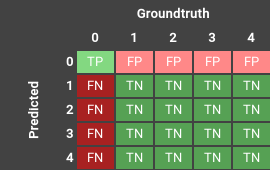
\includegraphics[width=\textwidth]{revue_litterature/confMat0}
		\caption{Classe 0}
	\end{subfigure}
	\hfill
	\begin{subfigure}{0.3\textwidth}
		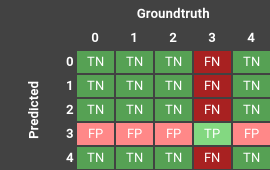
\includegraphics[width=\textwidth]{revue_litterature/confMat3}
		\caption{Classe 3}
	\end{subfigure}
\hspace{3em}
\caption{Définition de la matrice de confusion dans le cas multi-classes. Les images sont issues de captures d'écran prises sur notre outil d'interprétation des métriques de classification. Cet outil adopte une convention différente (transposée de la matrice de confusion). Les notions de Vrai Positif (\textit{True Positive (TP)}), Vrai Négatif (\textit{True Negative (TN)}) dépendent de la classe considérée.}
\label{fig:multiClassConfMatTool}
\end{figure}

\paragraph{Cas continu}
La plupart des réseaux de neurones, du fait d'être nécessairement différentiables, produisent une réponse continue. En utilisant une opération de type $\softmax$ ou sigmoïde, cette réponse s'interprète généralement comme la probabilité qu'associe le modèle à chacune des classes. La classe recevant la plus forte probabilité (dans le cas binaire, la classe associée à $p>0.5$) est celle prédite. Dans une certaine mesure, cette probabilité représente une mesure de confiance du modèle dans sa prédiction. Précisons que cette hypothèse est cependant contestée, par exemple par Gal et al. \cite{galDropoutBayesianApproximation2015} qui proposent une autre définition de l'incertitude du modèle. Quoiqu'il en soit, un modèle $A$ qui prédit correctement une classe avec $p_A = 0.95$ est intuitivement plus performant qu'un modèle $B$ faisant la même prédiction correcte avec $p_B=0.6$. Or les métriques que nous avons décrites jusqu'à présent ne font pas cette distinction (dès lors que les prédictions entre $A$ et $B$ sont les mêmes). \\
Pour ce faire, nous introduisons deux métriques, reposant sur un postulat similaire. Nous décrivons celles-ci dans le cas binaire, mais comme nous l'avons vu, tout problème multi-classes peut se ramener au cas binaire et les métriques continues ne dérogent pas à cette règle. 
\paragraph{\ac{AUROC}} La sensibilité et la spécificité permettent de décrire entièrement la matrice de confusion normalisée par ligne d'un modèle. Dans le cas idéal du classifieur parfait, cette matrice de confusion normalisée est simplement l'identité. Inversement, un classifieur qui se trompe systématiquement obtient la matrice miroir de celle-ci. Dans le premier cas, le couple sensibilité/ spécificité vaut (100\%, 100\%) et (0\%, 0\%) pour le second. A priori, un modèle correctement entraîné obtiendra un couple de scores se situant quelque part entre ces deux extremums. Cela dépendra du seuil de confiance qu'on souhaite associer à la prédiction. Soit $p^{(+)}$ la probabilité associée à la classe positive émise par le modèle. Dans le cas binaire et par défaut, si $p^{(+)}>0.5$, on considère que la classe prédite est positive. La valeur de 0.5, bien qu'intuitive (c'est celle qui sépare bien l'espace des probabilités en deux valeurs égales), est arbitraire. La condition de prédiction de la classe positive peut ainsi se formuler sous la forme $p^{(+)}>s$, où $s$ est un seuil arbitraire: plus il est élevé, plus le nombre prédiction positive diminue (la sensibilité aura tendance à diminuer) et le nombre de prédiction négative augmente (la spécificité aura tendance à augmenter). Pour obtenir des métriques évoluant dans le même sens, on définit la fonction d'efficacité du récepteur -dite courbe ROC- comme:
\begin{equation}
	\text{ROC}(s) = (\text{sensibilité}(s), (1-\text{spécificité})(s))
\end{equation}
On peut condenser cette fonction paramétrique en un seul score en calculant l'aire sous la courbe de la fonction, aussi appelée  \ac{AUROC}:
\begin{equation}
	\text{AUROC} = \int_{s=0}^{1}\text{ROC}(s)ds
\end{equation}
Sur la figure \ref{fig:AUROC_Curves}, nous fournissons quelques exemples de courbes ROC typiques suivant la qualité du modèle. Le graphique \ref{fig:AUROC_alwaysWrong} représente notamment un modèle qui prédit systématiquement la classe opposée à celle attendue.
\begin{figure}[!h]
	\centering
	\begin{subfigure}{.49\textwidth}
		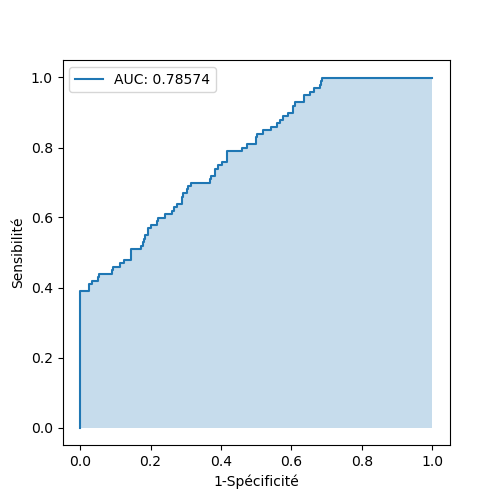
\includegraphics[width=\textwidth]{gnuplot/revue_litterature/AUC/mid_AUC}
		\caption{\textit{Bon} modèle}
	\end{subfigure}
	\begin{subfigure}{.49\textwidth}
		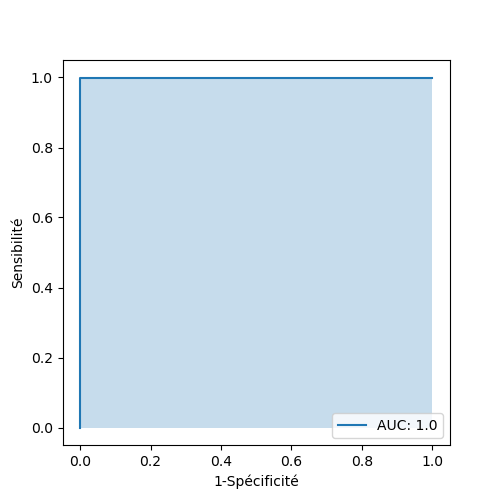
\includegraphics[width=\textwidth]{gnuplot/revue_litterature/AUC/perfect_AUC}
		\caption{Modèle idéal}
	\end{subfigure}
	\begin{subfigure}{.49\textwidth}
		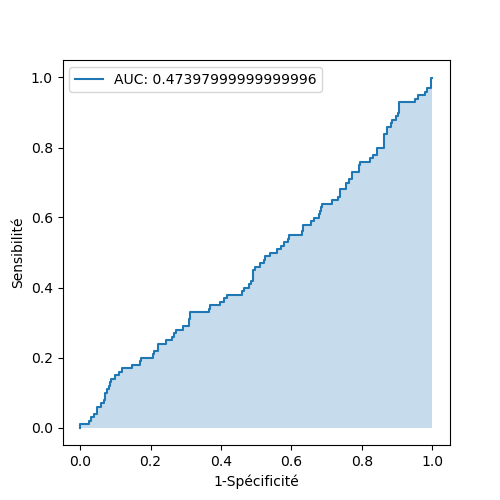
\includegraphics[width=\textwidth]{gnuplot/revue_litterature/AUC/random_AUC}
		\caption{Modèle faisant une prédiction aléatoire}
	\end{subfigure}
	\begin{subfigure}{.49\textwidth}
		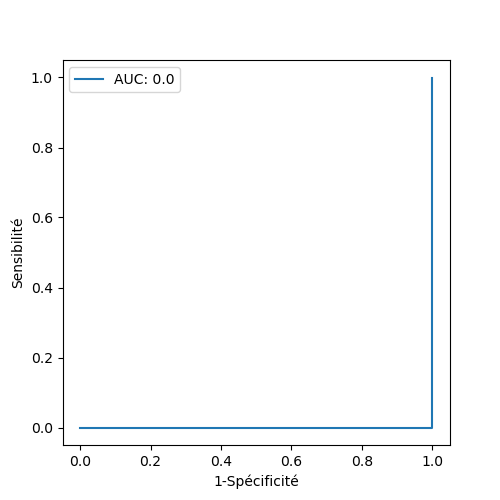
\includegraphics[width=\textwidth]{gnuplot/revue_litterature/AUC/worst_AUC}
		\caption{Modèle toujours faux}
		\label{fig:AUROC_alwaysWrong}
	\end{subfigure}
\caption{Exemples typiques de courbes ROC (et AUROC associés) pour différents types de modèles}
\label{fig:AUROC_Curves}
\end{figure}

\paragraph{Courbe Précision/Sensibilité} Exactement de la même manière que pour la courbe ROC, il est également possible de définir la courbe précision-sensibilité. À nouveau, on la synthétise en un seul nombre en extrayant de celle-ci l'aire sous la courbe. Cependant, pour cette métrique, il est courant de ne fournir qu'une approximation de cette aire suivant la méthode des rectangles simplifiant le calcul de l'intégrale. On parle alors de \textit{moyenne de précision} (\textit{Average Precision} en anglais, à comprendre dans le sens d'une moyenne sur la précision pondérée par la sensibilité) qui s'obtient suivant:
\begin{equation}
	\text{AP}  = \sum_n  = (\text{sensibilité}(s_n) - \text{sensibilité}(s_{n-1})) \cdot \text{precision}(s_n)
\end{equation}
Par rapport à l'AUROC, cette mesure présente l'avantage de bien mieux refléter le déséquilibre de classes grâce à sa dépendance à la précision. Un modèle possédant une forte sensibilité mais une faible précision tend à trouver tous les éléments positifs, mais au prix d'en détecter trop (d'où un nombre très important de faux positifs) et inversement. Cette capacité à détecter ce déséquilibre en fait une métrique appréciée dans le cadre des mesures de segmentation, en particulier pour des structures de petites tailles. Néanmoins, pour cette tâche, il existe des métriques spécifiques appréciées par la communauté que nous présentons maintenant.

\subsection{Segmentation sémantique}
La segmentation peut toujours se ramener à un problème de classification, par conséquent, toutes les métriques précédentes s'appliquent aussi ici; en gardant les mêmes considérations sur le choix judicieux de tel ou tel score en fonction des données (et notamment du déséquilibre de classes). Cependant, on attend aussi d'une métrique qu'elle possède un sens tangible et intuitif pour l'utilisateur. Cette intuition dépend des données et de la mesure: par exemple, si un modèle obtient une exactitude de 99.9\% mais que la classe positive ne représente que 0.1\% des pixels de l'image, cela ne dit rien de pertinent sur la performance du modèle (il peut n'avoir détecté aucun vrai positif). Dans ce cas de figure, l'exactitude se révèle une mesure contre-intuitive du fait du déséquilibre des données. Une mesure qui prend en compte ce déséquilibre n'est pas nécessairement plus intuitive: si le coefficient de Kappa de Cohen $\kappa$ d'un modèle est proche de 0, on saura de facto alors qu'il n'a obtenu aucun vrai positif. Mais un Kappa de 0.3, 0.5 ou 0.7, bien qu'indiquant certes une meilleure performances, n'est pas beaucoup plus informatif sur la tendance du modèle: fait-il de la sous ou de la sur-segmentation, rate-il une classe en particulier? \\
C'est pour ces raisons qu'il est courant d'utiliser des mesures dites géométriques pour quantifier la performance d'un modèle de segmentation. Ces métriques se basent en général sur la superposition de structures géométriques, les rendant ainsi visuellement intuitives. 
Formellement, on considère les pixels de la vérité terrain et ceux segmentées comme étant deux ensembles $X$ et $Y$. Pragmatiquement, sur des images, ces ensembles représentent bien des formes géométriques. 
\\
\paragraph{Indice de Jaccard}
Pour le calcul de l'indice de Jaccard, on définit alors le rapport de l'intersection sur l'union des deux ensembles:
\begin{equation}
	J(X, Y) = \frac{|X \cap Y|}{|X \cup Y|} = \frac{|X \cap Y|}{|X| + |Y| - |X \cap Y|}
\end{equation}
Par analogie avec les métriques de classification, on peut exprimer $|X \cap Y| = \VP$ et $|X| + |Y| - |X \cap Y| = \VP + \FP + \FN$. On obtient alors l'interprétation:
\begin{equation}
	J \approxeq \frac{\VP}{\VP + \FP + \FN}
\end{equation}
Dans la littérature, ce score est plus souvent référé comme étant l'IoU (de l'anglais \textit{Intesection-over-Union}) ou encore le mIoU (\textit{mean-IoU}) pour son équivalent multi-classe. 
\paragraph{Indice de Sørensen-Dice} Le coefficient Dice (tel qu'il est le souvent référé dans la littérature) est également une métrique très utilisée. Il s'obtient par:
\begin{equation}
	D(X, Y) = \frac{2|X \cap Y|}{|X| + |Y|}
\end{equation}
En reprenant l'analogie avec les notations de la matrice de confusion, on remarque que:
\begin{equation}
	D \approxeq \frac{2 \VP}{2\VP + \FP + \FN}
\end{equation}
C'est-à-dire le score F1. L'intérêt de cette métrique est donc essentiellement de procurer une interprétation géométrique du dit score.

\begin{figure}[!h]
	\centering
	\begin{subfigure}{.3\textwidth}
		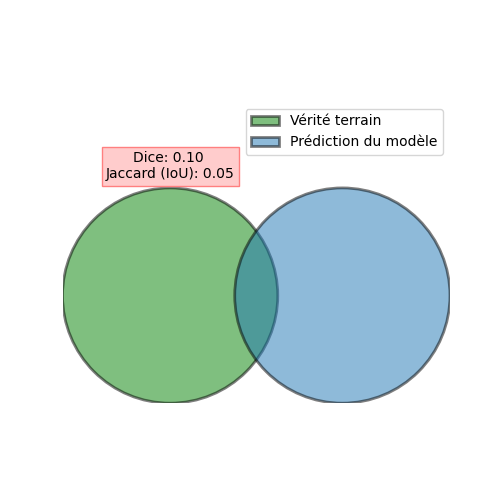
\includegraphics[height=13em]{gnuplot/revue_litterature/dice/bad_dice}
		\caption{}
	\end{subfigure}
	\begin{subfigure}{.3\textwidth}
		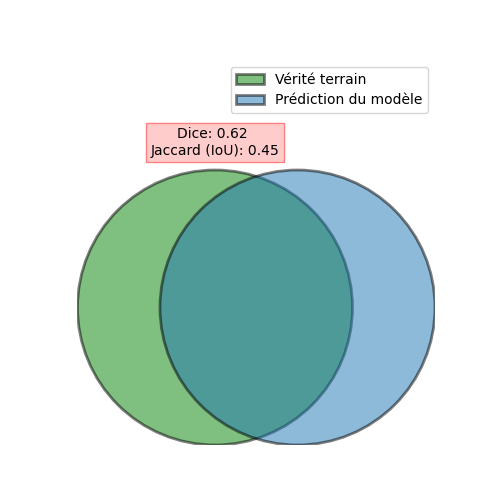
\includegraphics[height=13em]{gnuplot/revue_litterature/dice/mid_dice}
		\caption{}
		\label{fig:midDiceExemple}
	\end{subfigure}
	\begin{subfigure}{.3\textwidth}
		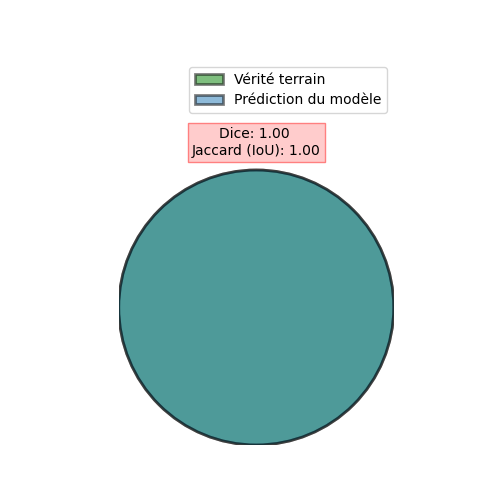
\includegraphics[height=13em]{gnuplot/revue_litterature/dice/perfect_dice}
		\caption{}
	\end{subfigure}
\caption{Évolution de l'indice de Jaccard et du coefficient de Sørensen-Dice sur trois cas de figure théoriques}
\label{fig:DiceJaccardExemple}
\end{figure}

Les deux mesures (Dice et indice de Jaccard) sont en réalité très similaire et évoluent dans le même sens. Il est d'ailleurs possible d'expliciter la relation qui les unit:
\begin{equation}
	D = \frac{2 \cdot J}{J+1}
\end{equation} 
L'étude de cette fonction nous renseigne notamment sur la double inégalité suivante:
\begin{equation}
	D / 2 \leq J \leq D
\end{equation}
Ces résultats se retrouvent bien sur l'illustration qu'on donne des deux métriques sur la figure \ref{fig:DiceJaccardExemple}. En résumé, on y observe bien que par rapport à l'indice Jaccard, le coefficient  de Dice accorde un plus gros poids aux éléments appartenant à l'intersection des ensembles, c'est-à-dire aux vrais positifs.
\subsection{Un outils dynamique pour appréhender les métriques}
Face à la multitude de métriques existantes, choisir celle(s) adaptée(s) au problème que l'on traite n'est pas trivial. Des travaux comme ceux de Maier-Hein et al. \cite{maier-heinMetricsReloadedPitfalls2022} fournissent bien une méthodologie de sélection, mais une fois le choix fait, l'interprétation d'une métrique donnée n'est pas forcément évidente pour autant. En particulier pour certaines applications où la notion de performances reste souvent vue comme relativement subjective: ainsi, pour la segmentation sémantique, un utilisateur aguerri peut en un coup d'\oeil{} comparer la prédiction à une vérité terrain. Or, l'appréciation qualitative ne rejoint pas forcément l'évaluation quantitative que fournit une métrique. Par exemple, sur la figure \ref{fig:midDiceExemple}, qualitativement, on pourrait croire à un indice de Jaccard relativement élevé; il n'est pourtant \og que \fg de 0.45. Ainsi nous arguons que pour interpréter un score, il est également nécessaire de se former à sa lecture sur des cas concrets, au delà de la compréhension du mode de calcul. À cette fin, nous avons développé une plateforme en accès ouvert sur internet visant à se familiariser sur les différentes métriques à travers des cas concrets manipulables. L'outils est conçu à des fins pédagogiques et se concentre sur la segmentation sémantique (une capture d'écran est fournie sur la figure \ref{fig:ScreenshotMetricTool}). Depuis sa publication initiale, deux modules ont été ajoutés, pour traiter des métriques de classification générale et celles concernant les séquences temporelles \footnote{L'outils est accessible à l'adresse suivante (sur ordinateur uniquement): \url{https://clementpla.github.io/SegmentationMetricTutorial/welcome}}.
\begin{figure}[h]
	\centering
	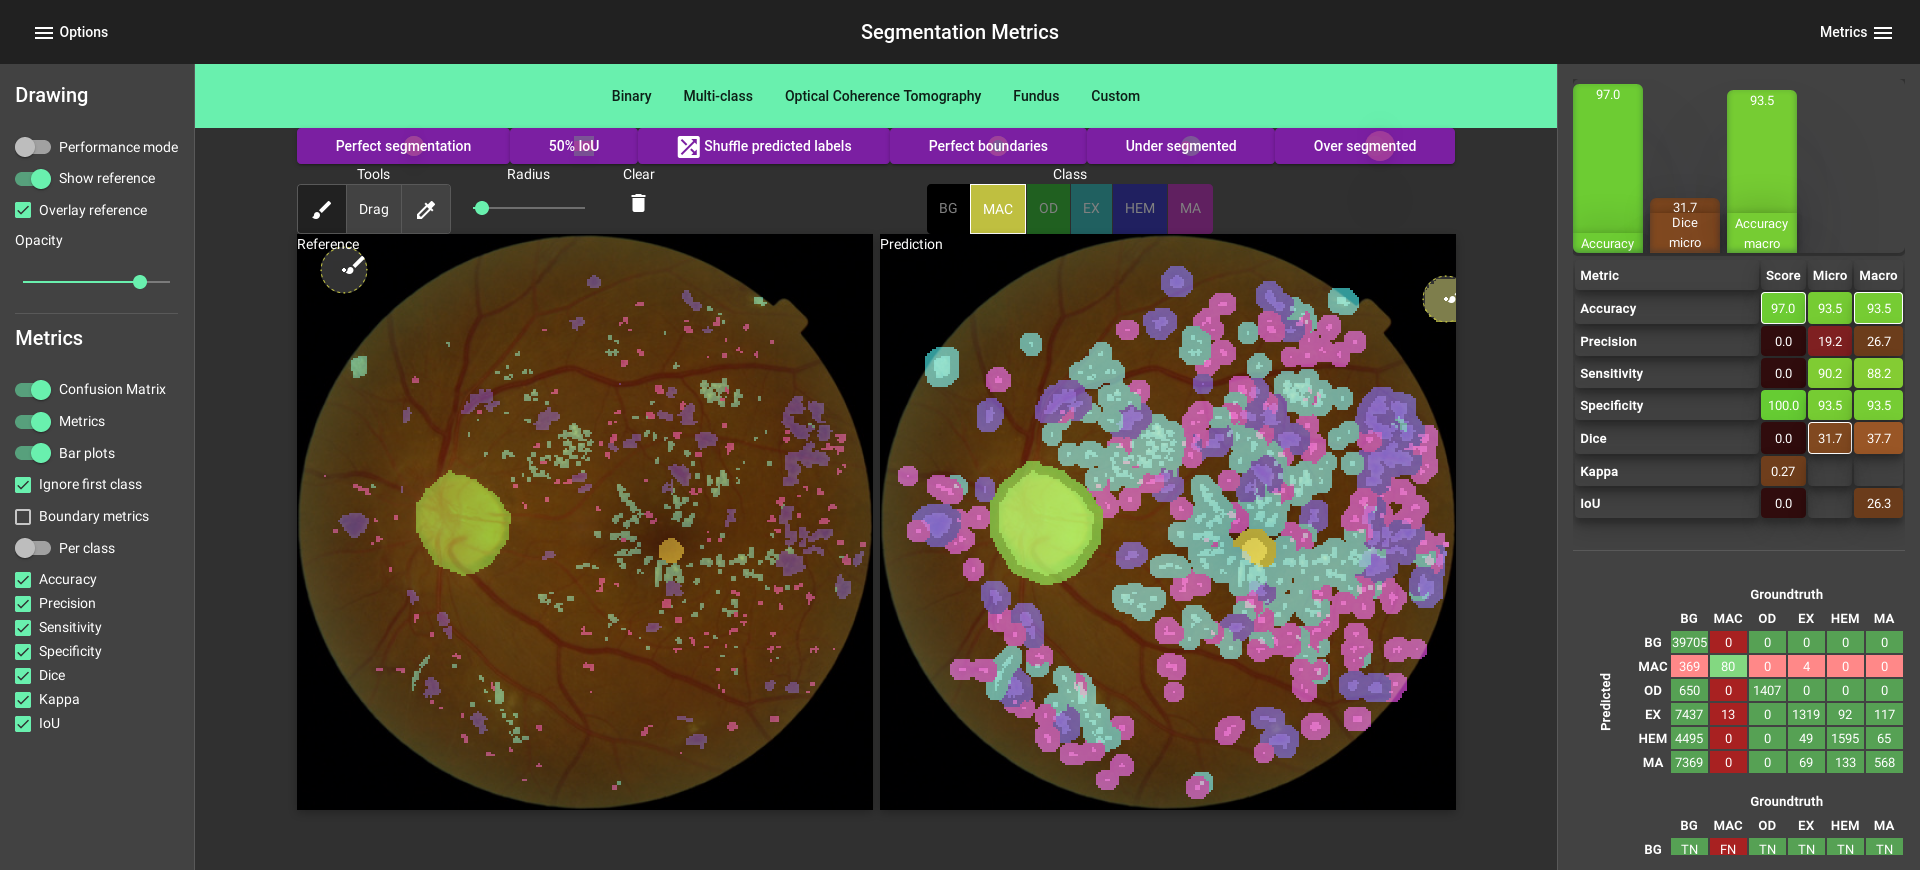
\includegraphics[width=.9\textwidth]{revue_litterature/interfaceMetric}
	\caption{Outils interactif de visualisation des métriques de segmentation. L'utilisateur se voit présenter deux canevas sur lequel il peut dessiner (à gauche, la vérité terrain et à droite, la "prédiction"). Les métriques sont actualisées en fonction des tracés pour illustrer leur évolution. Plusieurs scénarios pré-établis sont configurés pour illustrer les forces et les faiblesses de différentes métriques implémentées.}
	\label{fig:ScreenshotMetricTool}
\end{figure}


\newpage
\section{Applications à l'ophtalmologie}
\label{sec:RevueLittOphtal}

Jusqu'à présent, cette revue de littérature a fourni un inventaire des concepts théoriques utilisés de près ou de loin dans les travaux de recherche menés au cours de cette thèse. Or, celle-ci s'inscrit dans un contexte médical: si les notions théoriques sur la conception d'architecture, de généralisation, d'interprétabilité et autres ont toutes été manipulées durant nos travaux, elles se sont inscrites dans un champs de recherche appliquée à l'opthalmologie. Or, ce champ plus spécifique a également vu de nombreuses innovations se développer. La suite de cette revue de littérature propose donc de les couvrir et d'aborder plus précisément les différentes recherches et applications de l'apprentissage machine déployées autours de l'imagerie rétinienne. 
\subsection{Segmentation des structures rétiniennes dans l'imagerie de \fundus{}}
\label{sec:segmentationFCCN}
Dans la pratique clinique, le diagnostic de la rétine se fait sur la base de l'analyse de biomarqueurs structurels dans l'imagerie de \fundus{} ou de l'\ac{OCT}. Ainsi, la présence de certaines lésions ainsi que leur distribution est un indicateur primordial de l´état d'avancement de certaines maladies. Mais l'analyse des structures normales de la rétine peut également révéler une anormalité, que ça soit dans le processus d'acquisition ou par rapport à l´état de santé du patient. Par exemple, le nombre d'embranchement visible dans l'arbre vasculaire peut servir d'indicateur de qualité de l'acquisition. Cette section propose un survol des méthodes proposées pour la segmentation de telles structures mais par esprit de synthèse, seules les approches les plus récentes sont introduites. L'accent est mis sur le \fundus, notamment car il s'agit de la modalité la plus facile d'accès et la plus proche de nos travaux.

À l'instar de l'ensemble des publications récentes en vision par ordinateur, l'écrasante majorité des travaux de ces dernières années sur la segmentation sémantique de l'imagerie de 
\fundus{} s'appuient sur des réseaux de neurones convolutif. La prédominance de ce modèle unique ne doit pas masquer l'existence en pratique de très nombreuses contributions originales visant à l'ajuster aux spécificités de la tâche. Mais en général, les types de réseau proposés suivent toujours les grands principes des architectures fondatrices présentées en section \ref{sec:ModeleSegmentation}. En revanche, de nombreuses recherches se concentrent sur l'optimisation en elle même, par exemple par l'introduction de fonctions de coûts adaptées aux contraintes des données.
\\ 
Les premières publications dédiées à la segmentation de lésions rétiniennes ont en commun de ne se concentrer que sur un seul type de lésions. En 2016, Van Grinsven et al. \cite{vangrinsvenFastConvolutionalNeural2016} proposent un simple réseau (type LeNet) pour la segmentation des hémorragies rétiniennes, reposant sur un principe de classification par patch (présence ou absence). Du fait de leur inefficience, ce type de modèle est aujourd'hui complètement dépassé en faveur des équivalents totalement convolutif (et donc faisant de la classification par pixels). Chudzik et al. \cite{chudzikExudateSegmentationUsing2018} proposent une architecture utilisant le modèle de l'\textit{Inception Block} (voir figure \ref{fig:InceptionBlock}) visant à segmenter les exsudats dans des patchs d'images de \fundus{}. Les performances sont évaluées sur la base de données E-Ophtha et mettent particulièrement en exergue l'appartance du transfert d'apprentissage (y compris via pré-apprentissage sur des petites bases de données). Les mêmes auteurs proposeront plus tard \cite{chudzikExudatesSegmentationUsing2018} un nouveau modèle hybride composé d'un réseau convolutif utilisé d'une part pour fournir une carte de segmentation et d'autre part l'extraction d'un vecteur caractéristiques duquel est dérivé un score de proximité entre l'image d'entrée et sa plus proche voisine dans la base d'apprentissage. 
\\
À notre connaissance, le travail que nous avons mené au tout début de ce doctorat (initialement dans \cite{playoutMultitaskLearningArchitecture2018} puis prolongé dans \cite{playoutNovelWeaklySupervised2019}) est la première publication portant sur la segmentation multi-classes (dite aussi sémantique) par réseaux de neurones des lésions visibles au \fundus{}. Pour ce travail, l'architecture utilisée s'inspire du U-Net (voir section \ref{par:Unet}) à double décodeur. Chacun d'eux est chargé de la segmentation respective des lésions sombres (hémorragies, micro-anévrismes) et des lésions claires (drusen, exsudats durs et doux). Cette méthodologie propose également une approche originale de l'exploitation de données faiblement labellisées (c'est à dire pour lesquelles on ne dispose que du diagnostic et non des cartes d'annotations de lésions). L'article, bien que démontrant globalement des performances élevées en terme de segmentation, conclue sur la nécessité de constituer des bases de données plus conséquentes. Par ailleurs, la discrimination en deux classes seulement des lésions (sombres ou claires) est critiquable pour son manque de finesse. Il n'empêche que ce travail fut riche en enseignements sur les difficultés spécifiques à la tâche. Celles-ci n'auront cesse de motiver de nouvelles améliorations en terme d'architecture de réseaux de neurones dans les travaux subséquents. On peut citer notamment:
\begin{itemize}
	\item La difficulté de segmenter des structures ayant une grande variabilité de forme, de texture et de taille. Cette disparité pose de nombreux problèmes, y compris aux annotateurs humains.
	\item La présence de lésions potentiellement extrêmement petites (quelques pixels de large) parmi des images de très hautes résolutions. Outre la difficulté d'extraire un signal contrasté pour ces lésions parmi le bruit de fond, cela entraîne un très fort déséquilibre de classe auquel les techniques d'apprentissage statistiques sont très sensibles.
	\item L'absence de standard approprié pour évaluer la qualité d'une segmentation sémantique sur des structures aussi diverses.
	\item Un nombre généralement très faible de données d'entraînement comparativement à d'autres domaines d'applications des réseaux de neurones.
\end{itemize}
Plusieurs travaux ont depuis été publiés, prenant en compte un plus grand nombre de classes dans leur modèle et traitant de ces problématiques. Par ailleurs, plusieurs équipes ont également joint leurs données aux publications, offrant à la communauté de nouvelles bases de données publiques avec annotations réalisées par des médecins.
Les travaux de Xu et al. \cite{xuFFUNetFeatureFusion2021} étendent le principe d'une architecture U-Net à une problématique multi-classes. En l'occurence, tout comme pour la majorité des travaux qui seront détaillés dans cette section, quatre classes sont considérées:
\begin{enumerate}
	\item Les exsudats (parfois également appelés \textit{exsudats durs})
	\item Les hémorragies
	\item Les micro-anévrismes
	\item Les exsudats doux ou nodules cotonneux (\ac{CWS})
\end{enumerate}
Plusieurs modifications sont proposées pour améliorer l'architecture initiale: d'une part, chaque couche de l'encodeur est enrichie d'un module \textit{MSFF (Multiscale Feature Fusion)}, librement inspiré de l'\textit{Inception Block} décrit en section \ref{fig:InceptionBlock}. De plus, la fusion des caractéristiques entre le décodeur et l'encodeur s'appuie sur un modèle d'attention, là encore librement inspiré du module \textit{Squeeze \&  Excitation} (voir section \ref{par:squeezeNet}). On observe que l'utilisation d'une architecture multi-échelle est souvent présentée comme efficace pour gérer la variabilité de taille entre les lésions. Guo et al.  en intègrent le concept dans le réseau, surnommé L-Seg \cite{guoLSegEndtoendUnified2019}, reprenant une architecture de type VGG16 (voir la section \ref{par:VGG}) de laquelle sont extraites des cartes de caractéristiques à 5 échelle différentes. Celles-ci sont ensuite fusionnées indépendamment pour chacune des quatre classes considérées.
 
Yan et al. \cite{yanLearningMutuallyLocalGlobal2019a} introduisent un modèle intégrant à la fois le contexte global en moyenne résolution et le local en haute résolution. Pour cela, deux réseaux sont entraînés en parallèle, l'un sur l'image entière, l'autre sur un patch d'image extrait aléatoirement. Les caractéristiques extraites de ces deux modèles sont fusionnées par concaténation avant d'être transformées en carte de segmentation. Si les performances rapportées de ce double modèle sont très élevées, on peut noter que la reproductibilité de cet article est rendue difficile par son manque de précision (par exemple, les auteurs n'indiquent pas explicitement s'ils ont entraîné leur modèle sur chaque lésion simultanément ou individuellement). \\
Guo et al. proposent une architecture similaire, nommée CARNet \cite{guoCARNetCascadeAttentive2022}, visant à raffiner une segmentation globale (faite sur l'image entière) avec une segmentation par patchs en haute résolution. Mais à la différence de Yan et al. \cite{yanLearningMutuallyLocalGlobal2019a}, la fusion des caractéristiques est faite à chaque couche de l'architecture de décodage, par un mécanisme nettement plus complexe reposant sur une pondération par attention. Cette complexité architecturale, couplée à un code non publié et une méthodologie manquant de détails rend à nouveau la reproductibilité de cet article difficile.
\\

\paragraph{Bases de données} Une des difficultés de la segmentation sémantique du \fundus{} est liée à la diversité des images, due à des facteurs aussi divers que l'ethnicité des patients, leur état de santé (ainsi, une cataracte tend à assombrir l'image), le matériel d'acquisition etc. À cela s'ajoute que les lésions observables sur la rétine sont de formes, couleurs et textures très variables, ce qui rend leur annotation manuelle particulièrement laborieuse et coûteuse. Ces deux constats (diversité des images, difficulté d'annotations) rendent très précieuses les bases de données publiées qui sont au fondement d'un très grand nombre d'article de recherche. Cinq bases de données se démarquent, notamment en raison de leur inter-compatibilité supposée (c'est-à-dire qu'elles possèdent les mêmes classes d'annotations):
\begin{enumerate}
	\item \ac{DDR}, publiée par Li et al. \cite{liDiagnosticAssessmentDeep2019a}. Dans leur étude, les auteurs évaluent les performances de réseaux existants sur la classification de la rétinopathie diabétique et la segmentation des lésions, obtenant des performances modérées sur cette dernière tâche.
	\item \ac{FGADR}, publiée par Zhou et al. \cite{zhouBenchmarkStudyingDiabetic2021}. Il s'agit de la plus grande base de données publique annotées.
	\item \ac{IDRiD}, publiée à l'occasion d'une compétition organisée par Porwal et al. \cite{porwalIDRiDDiabeticRetinopathy2020}. 
	\item Retinal Lesions, publiée par Wei et al. \cite{weiLearnSegmentRetinal2021}. Les auteurs proposent par ailleurs une architecture multitâches, capable de simultanément segmenter les lésions et classifier la rétinopathie diabétique.
	\item Messidor, publiée par Decencière et al. \cite{decenciereFEEDBACKPUBLICLYDISTRIBUTED2014b}, cette base est à l'origine dédiée à la gradation de la rétinopathie diabétique. Au cours de cette thèse, un panel d'experts ont ré-annoté 200 images issues de cette base pour un ensemble de biomarqueurs (lésions et structures normales). 
\end{enumerate}

Une comparaison détaillée de ces différentes bases est proposée dans le chapitre \ref{sec:ChapitreSegmentation}. Notons simplement qu'elles se distinguent les unes des autres par leur taille, leur qualité et la finesse des annotations réalisée par les experts.
\subsection{Classification de l'imagerie rétinienne}
La première publication portant sur le diagnostic automatisé de l'état d'un \fundus{} 
remonte à 1976, détaillant une étude de Yamamoto et Yokouchi \cite{yamamotoAutomaticRecognitionColor1976b}. Leur système, semi-automatique, vise à classifier les croisements veines/artères. Le processus n´étant pas entièrement automatisé, un clinicien est tout d'abord chargé d'identifier la zone de croisement. L'algorithme va alors extraire les contours des vaisseaux, puis en dériver un diagnostic par la mesure du ratio des diamètres de la veine et de l'artère. Si cette méthode algorithmique est excessivement simple (selon les standards contemporains), il est intéressant de noter que certains points abordés restent très actuels; en particulier le traitement de la variabilité des couleurs existante entre plusieurs images de \fundus, variabilité qui à l'époque tirait son origine de la pellicule choisie pour l'acquisition, mais qui aujourd'hui dépend principalement du type de capteurs ou de l'ethnicité du patient. La difficulté que présente cette variabilité au sein des images (liée à l'acquisition, mais aussi anatomique) explique l'important travail de recherche sur cette modalité depuis cette première étude. Encore aujourd'hui, cet effort de recherche ne s'est pas relâché.
Et si l'\ac{OCT} n'existait pas encore à l'époque, il s'agit aujourd'hui d'un instrument communément utilisé. La suite de cette section traitera par conséquent à la fois des travaux menés sur le \fundus{} et ceux portant sur l'OCT. Elle sera divisée par ailleurs en deux axes.
Le premier aborde la question du diagnostic rétinien par approche globale. Dans cette catégorie est incluse toute méthode qui ne s'appuie pas sur la reconnaissance explicite d'une structure (saine ou pathologique) anatomique. Une approche de classification de maladies reposant sur des caractéristiques mathématiques (texture, fréquences, contours...) est considérée comme globale. À l'inverse, la section suivante abordera le diagnostic par approche locale, c'est à dire par la segmentation préalable de marqueurs anatomiques pour établir un diagnostic. Dans le cas de la rétinopathie diabétique par exemple, cela passera par la détection de lésions; pour le glaucome, par la segmentation complète du nerf optique, etc. A ce titre, cette approche sera également qualifiée d'ascendante, car allant d'échelle locale (c'est-à-dire au niveau du pixel) pour remonter à une prédiction globale (au niveau de l'image). La différence fondamentale avec l'approche globale réside par conséquent dans le fait d'associer localement un sens à chaque pixel (ou région de pixels) de l'image. Le diagnostic se fait donc par relation causale: \textit{Tel(s) marqueur(s) identifié(s) détermine(nt) tel diagnostic}.
\\
Ces deux catégories permettent de distinguer les modèles globaux, purement statistiques, des modèles locaux, reposant sur une connaissance biologique/médicale a-priori. Pour autant, il existe des modèles inversant l'approche globale (partant de modèles purement statistiques pour essayer de retrouver des marqueurs locaux causaux), de telle sorte que cette distinction devra être nuancée. En particulier, une courte discussion sera consacrée aux modèles interprétatifs. En substance, ceux-ci illustrent bien ce mécanisme d'inversion: suite à une classification globale, le modèle est conçu pour proposer une explication locale: c'est-à-dire des marqueurs cliniquement interprétables.


\subsection{Approche statistique de la classification de pathologies}
L'approche statistique (ou globale) de la classification de pathologies repose sur le présupposé que non seulement les données sont intrinsèquement statistiquement classables grâce à leur seul contenu mais surtout qu'il n'est pas nécessaire de baser cette classification à une pré-identification de certaines structures locales spécifiques via une expertise externe (autrement dit via un savoir a priori). L'algorithme développe cette expertise en construisant lui-même la représentation statistique adaptée à chaque classe de diagnostic. Les plus modernes, basés sur des réseaux de neurones pour la plupart, excellent généralement à cette tâche. Cependant, l'approche globale se heurte à deux obstacles principaux:
\begin{itemize}
	\item Pour apprendre une représentation de la distribution de chaque classe que l'on souhaite identifier, on estime nécessaire de disposer d'un nombre important de données, représentatif de tous les cas possibles. La capacité de généralisation sur un cas clinique non-prévu durant l'apprentissage est incertaine.
	\item L'acceptabilité clinique d'une telle solution, fut-elle validée  quantitativement, est limitée par l'absence d'interprétation accompagnant la prédiction.
\end{itemize}
Cette section parcourt une brève revue générale de différentes solutions proposées sur les deux modalités que sont le \fundus{} et l'\ac{OCT}.

\subsubsection{Méthodes classiques pour l'imagerie de \fundus{}}

Traditionnellement (c'est-à-dire avant les réseaux de neurones) la classification de maladies repose sur une méthodologie en deux étapes: la première consiste à extraire des caractéristiques discriminantes de l'image et la seconde à classifier ces caractéristiques dans les catégories diagnostiques (typiquement sain/malade dans le cas binaire, sain/grade 1/grade 2/.../grade n pour l'estimation de la sévérité ou bien sain/maladie 1/maladie 2/.../maladie n dans le cas multi-classes). Les caractéristiques peuvent être extraites automatiquement (pour les approches reposant sur un apprentissage  de bout en bout) soit en utilisant des modèles mathématiques traduisant l'image en une somme d'informations jugées les plus pertinentes (c'est à dire discriminantes) pour l'étape de classification. Cependant, pour bien distinguer cette dernière de l'approche locale
(décrite dans la section \ref{sec:approcheLocale}), spécifions d'emblée que ces caractéristiques ne correspondent pas à des structures anatomiques définies. De ce fait, l'étape d'extraction de caractéristiques ne peut et n'est pas évaluée par rapport à une base de données annotées par des experts. Par conséquent, seul le résultat final de classification est évalué par rapport à la vérité terrain. \footnote{Cette définition peut mener à des cas ambigus, où des caractéristiques anatomiques sont extraites (par exemple, la segmentation des microanévrismes) mais où les performances de segmentation ne sont pas quantifiées, c'est à dire une approche locale sans comparaison avec une annotation clinique au niveau du pixel. Auquel cas, seule la classification est réellement évaluée, mais ces travaux seront cependant considérés comme appartenant à l'approche locale.} \\ 
En dehors des réseaux de neurones convolutifs (permettant un apprentissage de bout en bout incluant l'extraction de caractéristiques), les principales méthodes d'extraction de caractéristiques reposent sur l'analyse spectrale et/ou texturale. On citera Guo et al. \cite{guoComputeraidedHealthcareSystem2015}, proposant une méthode de classification de la sévérité de la cataracte, entraînée et évaluée sur 445 images de \fundus. Les caractéristiques employées sont les coefficients caractéristiques de la transformation en ondelettes de Haar de l'image, combinés à une transformation en cosinus discrets de celle-ci. La classification se fait par analyse factorielle discriminante de Fisher. 
Acharyau et al.\cite{acharyauApplicationHigherOrder2008} proposent d'utiliser les moments statistiques spectraux d'ordre élevé (le moment d'ordre 0 étant la moyenne, celui d'ordre 1 la variance) pour caractériser une image, selon une technique issue de la théorie du traitement du signal.  Le vecteur résultat est utilisé pour la classification des quatre stades de la \ac{RD} en utilisant une \ac{SVM}. Une approche similaire est proposée à nouveau par Acharyau et al.\cite{acharyaIntegratedIndexIdentification2012}, proposant une classification basée sur la classification de textures du \fundus{}. Deux types de caractéristiques de textures sont utilisées. La première découle de l'utilisation de la matrice de co-occurrence de l'image (de laquelle sont dérivées des mesures de contraste, d'homogénéité, d'entropie...), la seconde utilise des statistiques d'ordre plus élevées. A nouveau, un classifier \ac{SVM} est utilisé pour distinguer les stades de la rétinopathie. Chowriappa et al.\cite{chowriappaEnsembleSelectionFeaturebased2013} proposent une approche similaire pour la classification de la maculopathie diabétique (plus exactement, la classification des \oe{}dèmes maculaires comme cliniquement significatifs ou non). Cependant, les informations texturales extraites sont différentes (dimension fractale, \ac{LBP}, ondelettes...). Par ailleurs, l'étape finale de classification repose sur un ensemble de quatre classificateurs (deux étant des variantes du classificateur Bayésien, le troisième un arbre de décision et le dernier une variante des \ac{SVM}).
\\ L'information texturale a également été employée pour d'autres maladies que la rétinopathie diabétique. Mookiah et al.\cite{mookiahLocalConfigurationPattern2015} proposent une variante des \ac{LBP}, nommée \textit{Local Configuration Pattern} pour distinguer les différentes classes de la \ac{DMLA}. 22 caractéristiques texturales sont extraites par image et classées par un ensemble de classificateurs (Arbre de décision, \ac{k-PPV}, classificateur Bayésien, Réseau de Neurones Probabilistes et \ac{SVM}). Les auteurs insistent particulièrement sur la sélection des caractéristiques et du classificateur optimaux. En particulier, l'effet de la taille du vecteur de caractéristiques est précisément quantifié.
\\
Pour le glaucome, Bock et al.\cite{bockGlaucomaRiskIndex2010} suggèrent une méthode basée sur une extraction de caractéristiques dans une région centrée autours du disque optique. Ces caractéristiques sont de trois types: un premier vecteur se compose simplement des intensités des pixels, un second est formée des coefficients de la transformée en série de Fourier et le troisième des coefficients B-splines (encodant la fréquence spatiale autours d'un pixel). Ces trois vecteurs sont individuellement compressés en utilisant l'\ac{PCA}. Un ensemble de classificateurs \ac{SVM} est utilisé pour évaluer la présence ou l'absence de glaucome. Entraîné et évalué (par validation-croisée) sur 575 images, l'algorithme obtient une sensibilité de 73\% pour une spécificité de 85\%. 
\bigbreak

\subsubsection{Classification du \fundus{} par réseaux de neurones}
\label{sec:fundusClassification}
Ces différents exemples donnent un aperçu des approches globales employées sur le \fundus{} en utilisant des modèles pré-définies d'extraction de caractéristiques. Bien que notre revue ne soit pas exhaustive, il est notable que le nombre de publications sur le sujet est relativement restreint par rapport à l'approche locale et l'approche globale par apprentissage profond. À l'inverse, pour celle-ci, la recherche menées ces dernières années est extrêmement prolifique.  Devant l'impressionnante quantité d'articles publiés sur le sujet\footnote{Une recherche sur le référenceur Google Scholar avec la combinaison de mots-clés \textit{deep learning, fundus, classification, diabetic retinopathy} couvrant la période 2019-2023 aboutit à 1610 articles publiés avec révision par les paires (13 300 tout type de publications confondu).}, plusieurs revues de littérature (y compris parues la même année) ont été proposées (par exemple \cite{aminReviewRecentDevelopments2016, jeongReviewMachineLearning2022, bilalSurveyRecentDevelopments2021, article, suriyasekeranAlgorithmsDiagnosisDiabetic2021, randiveReviewComputeraidedRecent2019, goutamComprehensiveReviewDeep2022} pour n'en citer que quelques-unes). Elles ont en grande partie constitué notre point d'entrée pour dresser cet inventaire.
\\
La vaste majorité des travaux que nous couvrons se basent sur des variations d'architectures de réseaux de neurones convolutifs.
Pour la rétinopathie diabétique,  Gulshan et al.\cite{gulshanDevelopmentValidationDeep2016} ont démontré la capacité d'un tel réseau a faire un dépistage des stades modérés et plus avancés de la rétinopathie diabétique. Le principal intérêt de cette étude est d'avoir mené l'évaluation de leur méthodes sur un jeu important de données (\SI{11171}{images} provenant de \SI{5871}{patients}). En obtenant une sensibilité de 97.5\% et une spécificité de 93.4\%, les auteurs ont démontré la viabilité clinique des réseaux de neurones, ces performances étant comparables voire supérieures à celles d'un ophtalmologiste. Gargeya et al.\cite{gargeyaAutomatedIdentificationDiabetic2017} ont confirmé ces résultats par une approche très semblable sur le même jeu de données; la différence étant l'utilisation de la validation-croisée et une architecture de classification légèrement différente.
Pratt et al.\cite{prattConvolutionalNeuralNetworks2016} ont mené une étude similaire, en entraînant cette fois leur algorithme à faire de la classification du grade de la \ac{RD} (et non juste du dépistage), suivant l'échelle \ac{ETDRS}. Les résultats obtenus sont en revanche relativement peu concluants: la spécificité obtenue est de 95\% pour une sensibilité de 30\%; on note notamment une incapacité complète du réseau à distinguer la classe \og \ac{RD} légère\fg, systématiquement confondue avec les classes \og Saine\fg et \og Modérée\fg. 
Ting et al.\cite{tingDevelopmentValidationDeep2017} proposent une approche basée sur un ensemble de réseau (entraînés en parallèle) visant à détecter plusieurs maladies conjointement. Les quatre prédictions produites concernent le dépistage de la \ac{DMLA}, d'un potentiel glaucome, de la \ac{RD} de stade modérée (ou plus) et de la \ac{RD} évoluée au stade de menace pour la vision du patient. Pour l'ensemble de ces classifications, les résultats obtenus sont légèrement en deçà à ceux des cliniciens expérimentés. Le système résultant est validé sur un ensemble de dix bases de données différentes provenant de communauté hétérogènes. Pour le dépistage de la \ac{RD} (premier  stade), les performances varient pour la sensibilité entre 97.1\% et 100 \% pour une spécificité allant de 73.3\% à 92.2\%. Pour un stade plus avancée \ac{RD} menaçant la vision, le système obtient un score de détection d'\ac{AUC} sensibilité/spécificité de 95.8\%. Pour la suspicion de glaucome, ce même score est de 94.2\% et de 93.2\% pour la \ac{DMLA}. 
Li et al.\cite{liEfficacyDeepLearning2018} proposent également un réseau de neurones pour détecter la présence de marqueurs du glaucome dans le \fundus{}, évaluée sur \SI{8000}{images} extraites d'une base de données de \SI{48116}{images}. La sensibilité (respectivement spécificité) obtenue est de 95.6\% (resp. 92 \%), pour une \ac{AUC} de 98.6\%. Une analyse des résultats obtenus par le réseau de neurones montre que la principale source d'erreurs de classification (faux négatifs et faux positifs) provient de l'existence d'une autre pathologie présente dans le \fundus{}, en particulier une forte myopie, une \ac{RD} et/ou une \ac{DMLA}. \\
Plus récemment, une étude similaire a été publiée par Sahlsten et al.\cite{sahlstenDeepLearningFundus2019}. Les auteurs approchent le problème en concevant une architecture permettant la classification des cinq classes de \ac{RD} ainsi que de quatre classes d'\ac{OMD}, en utilisant une base de données plus restreintes (mais quand même composée de 28512 images d'entraînement). La principale contribution de ce travail est d'évaluer l'importance de la résolution des images d'entrées dans la classification des maladies. Les auteurs proposent une étude comparée sur des résolutions allant de $256 \times 256$ jusqu'à $2095 \times 2095$, ce qui est une résolution exceptionnellement élevée pour un \ac{CNN}. L'étude met en évidence l'importance de ces très hautes résolutions pour l'obtention de performances compétitives sur la détection des deux maladies.
Une étude de même ampleur a également été menée sur la classification de la \ac{DMLA} par Grassmann et al.\cite{grassmannDeepLearningAlgorithm2018a}. Le système entraîné se compose de six architectures de réseau de neurones conventionnelles (VGGNet, Inception, ...), dont les prédictions respectives sont agrégées par une forêt d'arbres décisionnels. En pratique, les auteurs ont distingué différents stades de la maladies liées à l'âge de la rétine (neuf stades différents et donc neuf classes, selon l'échelle de gradation de l'étude proposée par Davis et al.\cite{davisAgeRelatedEyeDisease2005}), trois classes de progression des derniers grades de la \ac{DMLA} et une classe dédiée aux images considérées non-évaluable (mauvaise qualité). Le modèle complet est entraîné sur 120656 images et évalué sur 5555 images issues d'une base indépendante. Les performances varient assez fortement en fonction des tranches d'âges et des données utilisées, mais le réseau obtient en moyenne une exactitude de 85.7\% (top-2, signifiant que parmi les deux classes prédites obtenant les scores les plus élevés se trouve la classe effective de l'image).
\\
La tendance actuelle visant à substituer les modèles auto-attentifs aux CNNs n'a pas épargné la classification du \fundus{}, avec un nombre relativement important de nouveaux articles adaptant le \ac{VIT} à la détection de la rétinopathie diabétique. La très récente revue de littérature proposée par Muchuchuti et al. \cite{muchuchutiRetinalDiseaseDetection2023} offre un aperçu des améliorations que cette architecture peut apporter \cite{wuVisionTransformerbasedRecognition2021, guClassificationDiabeticRetinopathy2023a, sunLesionAwareTransformersDiabetic2021b, adakDetectingSeverityDiabetic2023}. Les performances rapportées sont généralement de paire avec celles des architectures CNNs équivalentes (en nombre de paramètres ou d'opérations). En revanche, le mécanisme d'attention est très souvent plébiscité pour fournir des prédictions facilement interprétables.
\subsubsection{Tomographie par Cohérence Optique}
Comparativement au \fundus{}, l'état de l'art sur la classification automatique des images \ac{OCT} est relativement réduit, ce qui s'explique par le fait que la technologie soit nettement plus récente et cliniquement plus difficile à manipuler. En parallèle, là où les images de \fundus{} sont désormais à portée de main de tout chercheur, le nombre de données \ac{OCT} accessibles publiquement est considérablement plus restreint, ce qui peut constituer un obstacle à la recherche transdisciplinaire.
\\
De plus, la difficulté à interpréter les données \ac{OCT} a limité le nombre de travaux portant sur l'approche globale. En effet, les données étant généralement plus bruitées et moins contrastées que le \fundus{}, tout en étant plus volumineuse, l'accent est généralement porté sur la détection de marqueurs cliniquement interprétables (en particulier la segmentation des différentes couches rétiniennes).
Mais il existe cependant quelques exemples d'approches reposant sur une interprétation globale. Ces travaux suivent globalement la même trajectoire chronologique que ceux traitant du \fundus{} présentés dans la section précédente. Là où les premières études dérivaient d'abord des vecteurs caractéristiques extraites de l'image via des modèles empiriques paramétrés avant d'en faire la classification dans un second temps, la tendance actuelle porte de plus-en-plus à une classification automatique de bout-en-bout.
L'approche de Srinivasan et al.\cite{srinivasanFullyAutomatedDetection2014} appartient à cette première catégorie empirique. Pour faire la classification entre des patients sains, atteints d'\ac{OMD} ou de \ac{DMLA} les auteurs emploient un \ac{SVM} pour classer des vecteurs caractéristiques extraits de chaque \textit{B-scan}. Chaque vecteur est obtenu en calculant l'\ac{HOG}. Les \textit{B-scan} ont été préalablement pré-traités pour corriger le bruit Speckle ainsi que la courbe de la rétine (qui est une surface tridimensionnelle sphérique) projetée vers un plan. 45 patients ont contribué à l'étude. D'autres travaux remplacent l'\ac{HOG} par un vecteur basé sur les \ac{LBP} (éventuellement sous différentes variantes). Lemaitre et al.\cite{lemaitreClassificationSDOCTVolumes2016} les utilisent dans la détection des \ac{OMD} sur une cohorte de 32 patients. Dans ce cas, les \ac{LBP} sont calculés en prenant en compte le volume. La méthode obtient une spécificité de 93.7\% et une sensibilité de 81.2\%. Albarrak et al.\cite{albarrakAgerelatedMacularDegeneration} utilisent une combinaison des \ac{LBP} et des \ac{HOG} pour la détection de la \ac{DMLA}. Là encore, les caractéristiques sont extraites par sous-volumes et non par tranches. 140 acquisitions \ac{OCT} sont utilisées et le système atteint une spécificité de 90.5\% pour une sensibilité de 92.4\%. L'ensemble de ces études utilisent les \ac{SVM} comme classificateurs, ceux-ci étant connus pour être capable de généraliser de manière robuste y compris avec un petit nombre de données d'entraînements. 
\\
A contrario de ces approches exploitant ces vecteurs caractéristiques explicites, Lee et al.\cite{leeDeepLearningEffective2017a} sont les premiers à expérimenter une approche par \ac{CNN} (architecture VGG) pour le dépistage de \ac{DMLA}. L'étude est menée sur \SI{9285}{patients}, menant à un total de 43~328 acquisitions OCT centrées sur la macula. Le réseau entraîné obtient une sensibilité de 85.41\% pour une spécificité de 93.82\% sur 20\% de cette base de données préservées pour l'évaluation. Karri et al.\cite{karriTransferLearningBased2017} étendent ces travaux à une classification tri-classes, permettant en plus de la \ac{DMLA} de distinguer les \ac{OMD}. N'ayant accès qu'à 45 patients, les auteurs s'emploient à démontrer l'efficacité de l'apprentissage par transfert, en récupérant un réseau pré-entraîné à la classification d'images naturelles (non médicales). \\
La liste des travaux se basant sur l'apprentissage profond et les réseaux convolutifs pour la classification ne cesse de s'agrandir, élargissant le champs d'application et confirmant l'efficacité globale de ces algorithmes. Cependant, la conséquence néfaste de cette tendance est qu'il devient peu aisé de distinguer une contribution propre. A la lecture de la revue de littérature qui vient d'être donnée, deux points principaux sont à relever:
\begin{itemize}
	\item A notre connaissance, à l'exception des travaux de Muhammad et al.\cite{muhammadHybridDeepLearning2017}, il n'y a pas eu d'approche globale de la classification du glaucome. C'est un constat relativement étonnant: d'une part car cette approche a été testée sur le \fundus{} alors qu'il est reconnu que l'\ac{OCT} est particulièrement adapté au diagnostic du glaucome \cite{jaffeOpticalCoherenceTomography2004}. D'autre part, cette maladie étant relativement difficile à définir cliniquement comme une simple combinaison de symptômes pathologiques exclusifs, on s'attendrait à ce qu'une approche statistique basé sur l'apprentissage soit capable d'identifier des corrélations plus fines des marqueurs de la maladie. 
	\item Un certain nombre de travaux et en particulier ceux reposant sur l'apprentissage par \ac{CNN}, se limitent à l'étude de chaque \textit{B-scan} individuellement traité comme une image. Or l'\ac{OCT} donne accès à une représentation 3D, et même si des contraintes matérielles et techniques limitent les traitements numériques réalisables, on s'attend à ce que la prise en compte des informations volumiques renforcent la capacité prédictive d'un modèle. En particulier, l'utilisation d'un réseau convolutif tri-dimensionnel semble appropriée à la tâche de classification. 
\end{itemize}

\subsection{Du local au global: approche ascendante de la classification des pathologies par reconnaissance préalable des biomarqueurs anormaux}
\label{sec:approcheLocale}
Dans cette section seront présentés différents travaux reposant sur une décomposition de la détection de la maladie en deux étapes. La première est une étape de segmentation (ou de détection), visant à obtenir les contours (ou respectivement de trouver la région) d'une structure pré-définie et dont la connaissance permet de guider un diagnostic. La seconde étape consiste à analyser ces résultats de segmentation, d'en extraire des caractéristiques spécifiques et, suivant certaines règles cliniques ou statistiques, s'en servir pour établir le diagnostic d'une maladie donnée.
\subsubsection{Imagerie de \fundus{} par approche locale}
\label{sec:approcheLocaleFundus}



\paragraph{Glaucome}
La détection du glaucome dans l'image de \fundus{} repose en général sur la caractérisation du rapport entre le diamètre de la tête du nerf optique et celui de la papille (indicateur \ac{CDR}). Tel que mentionné dans la section \ref{sec:glaucome}, une augmentation du \ac{CDR} est un signe clinique (parmi d'autres) d'un potentiel glaucome. Cette métrique est l'exemple typique d'une approche par biomarqueur car pour la calculer, la première étape consiste à segmenter la papille et la tête de nerf optique. Wong et al.\cite{wongLevelsetBasedAutomatic2008} proposent une approche basée sur une approximation elliptique du disque optique, dont les frontières sont obtenues sur les intensités de l'image. La tête de nerf optique en est dérivée selon la même méthode, mais partant de la segmentation de la papille. 
De façon plus atypique, Muramatsu et al.\cite{muramatsuDetectionRetinalNerve2010} proposent de détecter les défauts dans la couche des fibres nerveuses -par projection des images dans un espace polaire, le filtrage de Gabor du résultat et la classification de zones candidates. Si la méthode semble fonctionner (en terme de sensibilité) sur les 162 images de l'étude, les auteurs pointent une tendance à produire un nombre important de faux positifs. Le \fundus{} n'étant pas la modalité la plus appropriée en clinique pour observer les couches profondes (comme celle des fibres nerveuses), il est intéressant qu'une analyse de textures permette malgré tout de détecter des traces de glaucome.
\paragraph{Rétinopathie diabétique} L'essentiel des méthodes utilisées pour la détection et/ou la gradation de la \ac{RD} repose sur une pré-segmentation des lésions, notamment les micro-anévrismes, et sur des heuristiques cliniques (nombre de lésions, répartition par rapport à la macula, type de lésions...) et nous renvoyons à la section \ref{sec:segmentationFCCN} pour une revue de littérature plus détaillée sur le sujet. Certaines approches ne reposent cependant pas sur la détection de lésions. C'est le cas de celle de Welikala et al.\cite{welikalaAutomatedDetectionProliferative2014}, qui proposent d'identifier le stade prolifératif de la \ac{RD} en se basant sur la carte du réseau vasculaire (obtenu par segmentation) dont est extrait un ensemble de caractéristiques. La segmentation des vaisseaux est obtenue par une variante du détecteur de ligne multi-échelle proposé par Nguyen et al.\cite{nguyenEffectiveRetinalBlood2013}. Ces caractéristiques propres au réseau vasculaire traduisent des informations topologiques et/ou morphologiques (nombre de pixels appartenant à  un vaisseau, nombre de segments, densité, orientations...). Le vecteur caractéristique obtenu est utilisé pour distinguer les images contenant des néo-vaisseaux et celles n'en contenant pas. Une approche similaire est employée par Christodoulidis et al.\cite{christodoulidisMultiscaleTensorVoting2016}, qui proposent une caractérisation des petits vaisseaux segmentés par une approche par tenseur. L'approche permet ainsi d'identifier localement les néo-vascularisations. \\
De cet exemple, on perçoit la pertinence d'un système complet pour la gradation de la rétinopathie diabétique, c'est à dire incluant à la fois une segmentation des lésions, mais également de l'arbre vasculaire.


\subsubsection{Imagerie \ac{OCT} par approche locale}

La détection de maladie par approche locale dans les images \ac{OCT} est généralement initiée par une étape de segmentation des couches rétiniennes, éventuellement des lésions, d'extraction de caractéristiques (notamment d'épaisseur) et d'une dernière étape de classification.

\paragraph{Rétinopathie diabétique} Cette approche est employée par Eltanboly et al.\cite{eltanbolyComputeraidedDiagnosticSystem2017a}, qui segmente 12 couches rétiniennes distinctes (ajoutant les zones d'interdigitation, ellipsoïde et myoïde et la membrane limitante externe à la liste dressée en section \ref{sec:AnatRetina}). La segmentation est obtenue par un un ensemble de règles relativement complexes, basées sur la transformation de l'image d'entrée en une carte de probabilités (en utilisant la théorie des champs aléatoires de Gibbs-Markov). Une fois les couches segmentées, des caractéristiques d'épaisseur, courbure et réflexivité en sont extraites puis classées par un réseau de neurones. 
\paragraph{Lésions}
Novosel et al.\cite{novoselJointSegmentationRetinal2017} sont les premiers à proposer une méthode de segmentation de lésions couplée à la segmentation des couches rétiniennes et obtenant les mêmes performances que l'état de l'art propre à chacune de ces deux tâches. Par ailleurs, leur approche ne repose pas sur des méthodes d'apprentissage machines, rendant, selon eux, la méthode plus facile à améliorer. Chaque couche (les lésions étant considérées comme une couche) est segmentée suivant une certaine équation de propagation. 
Fang et al.\cite{fangAttentionLesionLesionAware2019} proposent une méthode de classification des lésions maculaires (et non de maladie), également par une première étape de segmentation. La classification se fait par B-scan, parmi quatre classes (Drusen, \ac{OMD}, \ac{CNV} ou Saine). Le mécanisme présenté repose sur la notion d'attention (même si le terme est légèrement galvaudé ici, l'attention étant contrainte et non apprise). Un premier réseau est entraîné à identifier une région contenant une lésion (quel que soit son type). La prédiction de ce premier réseau est fournie en entrée d'un second, qui se chargera de classer le B-Scan, en étant conditionné par la pré-segmentation du premier réseau. Une idée similaire est proposée par Huang et al.\cite{huangAutomaticClassificationRetinal2019}, à travers un double \ac{CNN} de segmentation/classification. Un premier réseau pré-entraîné est chargé de segmenter les différentes couches rétiniennes ainsi que les masses fluides. Pour ce rôle, les auteurs ont choisi le ReLayNet, librement accessible et utilisable, proposé par Roy et al.\cite{royReLayNetRetinalLayer2017}. De la carte de segmentation obtenue sont extraites la couche située entre la \ac{RPE} et la membrane interne supérieure d'une part et d'autre part la couche située entre la \ac{RPE} et la membrane de Bruch. Chacune des deux couches est fournie à un second jeu de \ac{CNN}s, qui prédisent la présence de Drusen, d'\ac{OMD} et de \ac{CNV}.
%\paragraph{Glaucome} Asaoka et al.\cite{asaokaUsingDeepLearning2019a} proposent une approche basée sur l'extraction d'information d'épaisseurs de couches sur des images OCT et la classification par un \ac{CNN}. La première couche extraite correspond à l'épaisseur de la couche dans la région maculaire (c'est à dire de la couche ganglionnaire et la couche plexiforme interne combinées). La seconde consiste en la couche des fibres nerveuses. Les deux cartes d'épaisseur obtenues sont fournies au classificateur. Les auteurs comparent différentes approchent de classification, mais obtiennent leur meilleur score par transfert d'apprentissage sur un \ac{CNN} (sensibilité de 82.5\% et spécificité de 93.9\%).
%
%Les quelques travaux cités préalablement se bornent pour la plupart à la détection d'une maladie particulière (par exemple le glaucome), ou à l'extraction d'une seule structure prédéfinie (par exemple les interfaces rétiniennes). Observant cela, Fauw et al.\cite{fauwClinicallyApplicableDeep2018} proposent une méthode de classification cliniquement déployable, c'est-à-dire essayant de couvrir un panel de maladies le plus exhaustif possible. Devant la difficulté de la tâche, les auteurs ont choisi de découper leur approche en deux: un premier \ac{CNN} est entraîné à la segmentation sémantique d'un \textit{B-scans} en 15 classes différentes (incluant des lésions). Plus précisément, pour obtenir des segmentations satisfaisantes, un ensemble de réseaux \text{U-Net} sont entraînés à cette tâche. Cet apprentissage est mené de manière supervisée, grâce à 877 volumes \ac{OCT} sur lesquels 3 \textit{B-scans} ont été manuellement annotés. 
%La carte de segmentation obtenue est ensuite fournie à un second réseau, de classification cette fois, qui  génère à son tour deux types de prédictions. La première indique, parmi quatre classes, la nécessité de traitement du patient (\textit{Urgent, semi-urgent, routine, observation}). La seconde associe à chaque image un score de maladies (pour 14 maladies), permettant ainsi la classification multi-classes. Les performances obtenues atteignent un niveau impressionnant, comparable à celui d'un des six expert médical mis à contribution pour l'étude (\ac{AUC} supérieure à 99\% pour la plupart des pathologies). Plusieurs enseignements peuvent-être tirés de la discussion de l'étude:
%\begin{enumerate}
%	\item Obtenir une carte de segmentation au préalable de la classification présente plusieurs avantages, dont le premier est l'interprétabilité de la méthode, qui la rend déployable cliniquement. Par ailleurs, ce faisant, la classification est rendue indépendante de l'appareil d'acquisition.
%	\item Pour gérer la prédiction de multiples pathologies, il est pertinent de créer une architecture multi-classes (c'est-à-dire associant un score à chaque maladie plutôt qu'une classe).
%	\item Certaines structures sont incertaines à segmenter: une approche par ensemble de modèles permet, par effet moyenneur d'alléger cet effet.
%	\item Le modèle de segmentation a des difficultés à généraliser en dehors d'images acquises dans les mêmes conditions que celles de la base de données d'apprentissage. Combiner différentes bases d'apprentissage, issues de différentes machines d'acquisitions, entraîne de nettes améliorations des performances.
%	\item En annexe, les auteurs proposent une métrique permettant de quantifier la probabilité qu'un premier modèle A (par exemple: leur architecture) soit meilleur qu'un second modèle B (par exemple: un clinicien). Pour cela, ils proposent d'évaluer la notion de différence significative par test binomial. Pour chaque image, on considère que la probabilité de classification correcte par le modèle A (resp. B) est constante (mais inconnue) $p_A$ (resp. $p_B$). Sur l'ensemble de N images de test, si le modèle A (resp. B) obtient $k_A$ (resp. $k_B$) images correctement classifiées, (ce qui correspond à une probabilité d'occurrence de $Pr(k_A)=B(k_A|p_A, N)$) on peut estimer la probabilité que $p_A$ soit supérieure à $p_B$: $Pr(p_A>p_B|k_A, k_B, N)$. Les auteurs dérivent les équations pour calculer cette probabilité.
%\end{enumerate}




%\begin{figure}[htb]
%\centering
%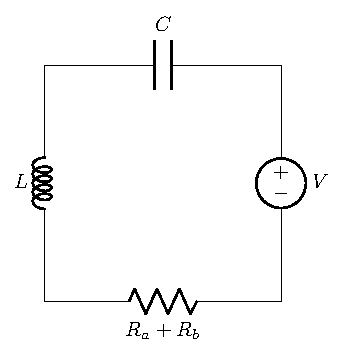
\includegraphics[width=2in]{Circuit_compile}
%\caption{Circuit}
%\label{fig:Circuit}
%\end{figure}  % Revue de littérature / Literature review
\Chapter{Segmentation des lésions rétiniennes dans l'imagerie de \fundus{}.}\label{sec:Theme1}
\label{sec:ChapitreSegmentation}


Pour le médecin, l'identification et à la quantification des biomarqueurs visibles dans l'image de \fundus{} est un préalable au diagnostic des maladies affectant potentiellement la rétine. En effet, les règles diagnostiques d'un grand nombre d'entre elles se basent sur la reconnaissance d'une ou plusieurs structures anatomiques et de leur analyse (topologie, nombre, texture etc.). Parce qu'elle illustre parfaitement ce concept, prenons la rétinopathie diabétique comme exemple: chaque grade de la maladie est caractérisé par un ensemble de marqueurs (essentiellement des lésions) dont l'évolution (en taille, nombre et type) est révélatrice de la progression de la gravité de la maladie \cite{boucherEvidencebasedCanadianGuidelines2020}. En pratique, cette identification est loin d'être aisée, y compris pour des cliniciens expérimentés. Qui plus est, le recours de plus en plus fréquent aux centres de télé-dépistages privent l'examinateur d'informations contextuelles lui permettant de résoudre certaines ambiguïtés. Nous illustrons dans la section \ref{sec:segmentationDifficulte} suivante  plusieurs des difficultés pouvant tromper y compris l'\oeil{} expert. À ce titre, confier la tâche à un algorithme est perçue comme une solution potentielle. L'identification des frontières des structures locales et la reconnaissance de celles-ci dans une image est appelée segmentation sémantique. Ce chapitre traite de la question de l'obtention des cartes de segmentation pour chaque grande classe de lésions existante dans le \fundus{}, mais aussi de l'exploitation de ces segments une fois ces cartes obtenues.

À travers notre revue de littérature sur le sujet (section \ref{sec:segmentationFCCN})  se dessine l'image d'un champs de recherche actif et massivement tourné vers la conception et l'optimisation de nouvelles architectures de réseaux de neurones. Pour subvenir aux besoins de cette recherche, de plus en plus d'équipes ont mis en accès libre leurs données pour un usage académique, ce qui représente souvent l'équivalent de plusieurs centaines d'heures de travail d'annotations réalisées par des experts. En revanche, rares (sinon inexistants) sont les travaux qui explicitent leur protocole d'annotations de manière détaillée et reproductible. Cela mène à des annotations inter-bases très hétérogènes, bien que représentant supposément les mêmes structures. À cela s'ajoute que chaque base de données représente une certaine population et a été acquise dans des conditions spécifiques (caméra, condition d'éclairage, acquisition mydriatique ou non...). Or, étant donnée la taille relativement réduite de ces bases, il apparaît clairement qu'une représentation exhaustive de toutes les spécificités du \fundus{} à travers une seule base confine à la gageure. Pourtant, il n'existe à notre connaissance aucun travail cherchant à combiner ces bases de données (que ce soit pour entraîner ou évaluer un modèle) ou même simplement à les caractériser respectivement. La littérature tend globalement à décorréler les travaux sur la segmentation en elle-même et les questions afférentes à la généralisation.
L'étude présentée dans ce chapitre propose donc de combler cette absence d'analyse comparative. Plusieurs objectifs de recherche vont venir préciser et élargir largement l'ambition initiale de ce travail et sont détaillés dans la section \ref{sec:SegmentationProblematique}. Pour délimiter notre étude, le choix a été fait de ne considérer que les cinq bases de données récentes les plus importantes. Par ordre de taille (i.e. de 
nombre d'images) celles-ci sont:
\begin{enumerate}
	\item \acf{IDRiD}\cite{porwalIDRiDDiabeticRetinopathy2020}.
	\item MESSIDOR \cite{decenciereFEEDBACKPUBLICLYDISTRIBUTED2014b}
	\item \acf{DDR} \cite{liDiagnosticAssessmentDeep2019a}
	\item RET-LES \cite{weiLearnSegmentRetinal2021}
	\item \acf{FGADR} \cite{zhouBenchmarkStudyingDiabetic2021}
\end{enumerate}
Une description détaillée de ces bases est proposée dans la section \ref{sec:variabilitéSegmentation}.
Ces jeux de données ont l'avantage d'avoir en commun certaines annotations de lésions spécifiques, sur lesquelles porte notre travail:
\begin{enumerate}
	\item \acf{EX} (également qualifiés d'\textit{exsudats durs})
	\item \acf{HEM}
	\item \acf{MA}
	\item \acf{CWS}
\end{enumerate}

Notre étude s'arrime donc à la tendance de la majorité des articles publiés qui se restreint à ces quatre lésions. Notons qu'il existe des travaux étendant leur portée à un plus grand nombre de lésions; en particulier pour la segmentation des ischémies et des néo-vascularisations \cite{weiLearnSegmentRetinal2021}, qui sont de toute première importance pour la classification des stades avancées de la rétinopathie \cite{boucherEvidencebasedCanadianGuidelines2020}. Mais notre étude se voulant comparative, il était nécessaire de se limiter au dénominateur commun en terme de classes traitées.


\subsection{Difficultés liées à la segmentation des lésions}
\label{sec:segmentationDifficulte}
Il est notoire - et les efforts continus de recherche en attestent- que la segmentation des lésions rétiniennes n'est pas une tâche aisée; même en faisant abstraction des difficultés liées à la disparité entre les bases de données. Nous recensons sur la figure \ref{fig:DifficultesAcquisition} un certain nombre de cas illustrant la complexité du problème, toutes les images étant issues de la même base RET-LES.  
\begin{figure}
	\begin{subfigure}[t]{.5\textwidth}
		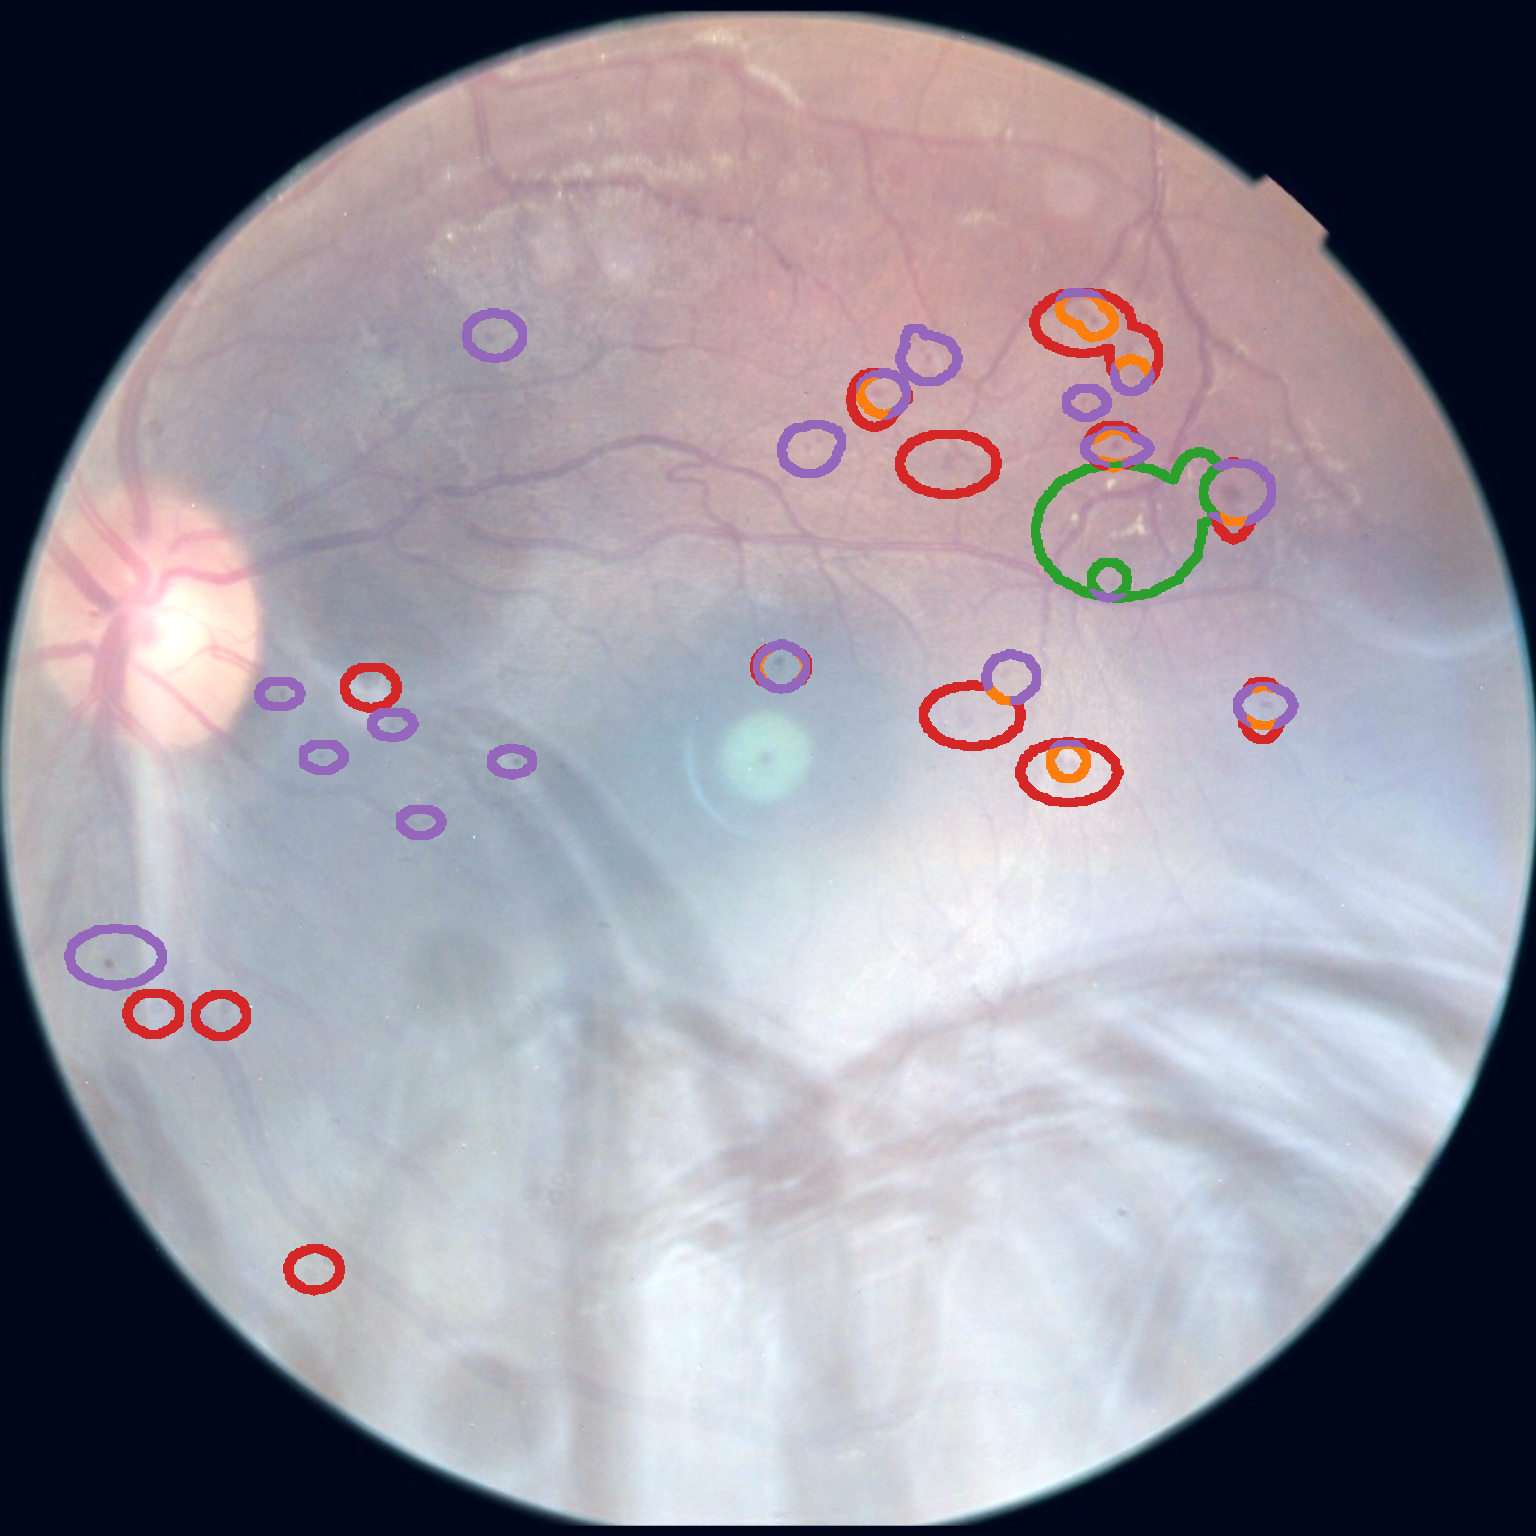
\includegraphics[width=\textwidth]{segmentation_lesions/difficultees/cil.png}
		\caption{Artefacts visibles dans la région inférieure (cils)}
	\end{subfigure}
	\begin{subfigure}[t]{.5\textwidth}
		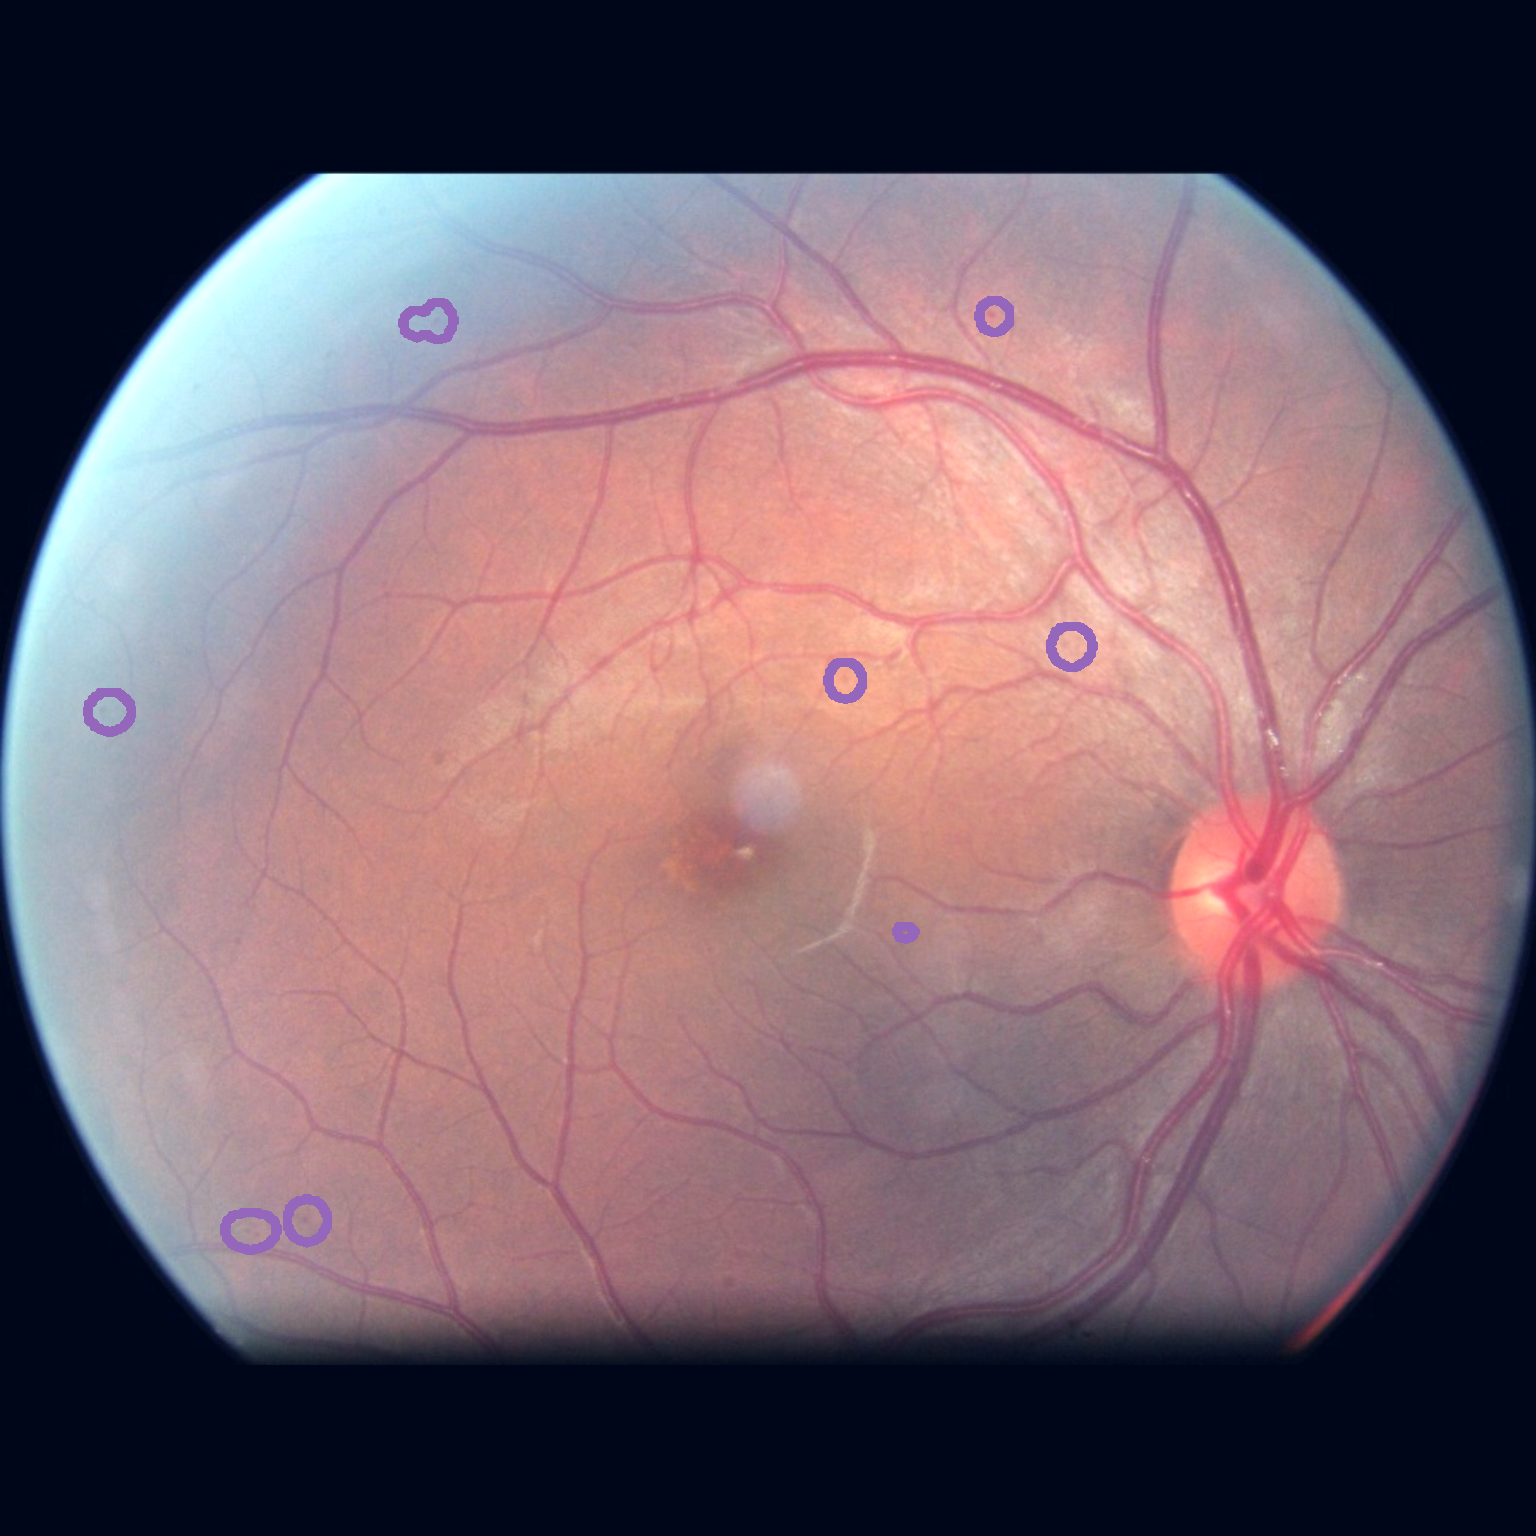
\includegraphics[width=\textwidth]{segmentation_lesions/difficultees/surexposition.png}
		\caption{Sur-exposition lumineuse qui sature le champ temporal de la rétine}
	\end{subfigure}
	\begin{subfigure}[t]{.5\textwidth}
		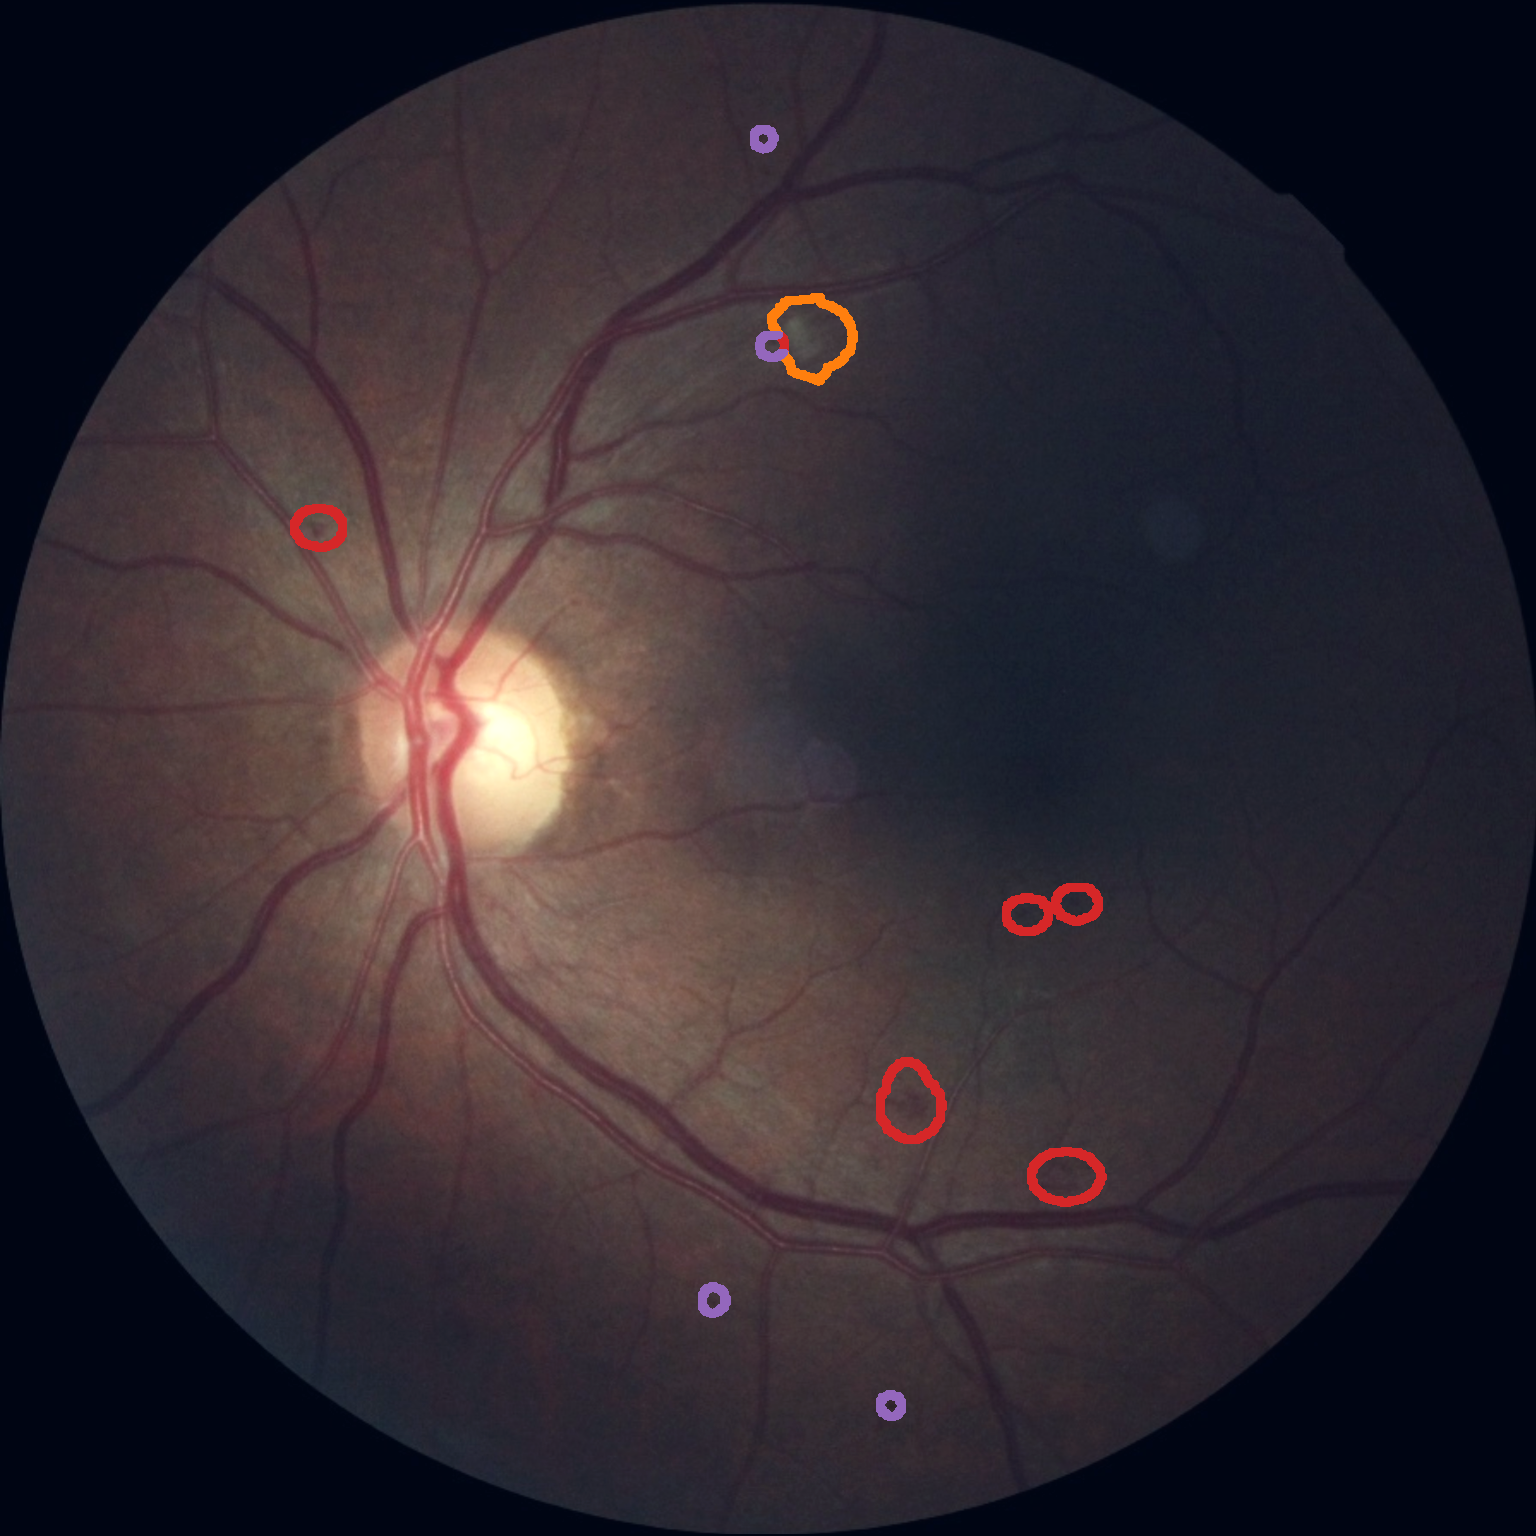
\includegraphics[width=\textwidth]{segmentation_lesions/difficultees/sombre.png}
		\caption{Sous-exposition globale compliquant la lecture de la périphérie temporale supérieure de la rétine}
	\end{subfigure}
	\begin{subfigure}[t]{.5\textwidth}
		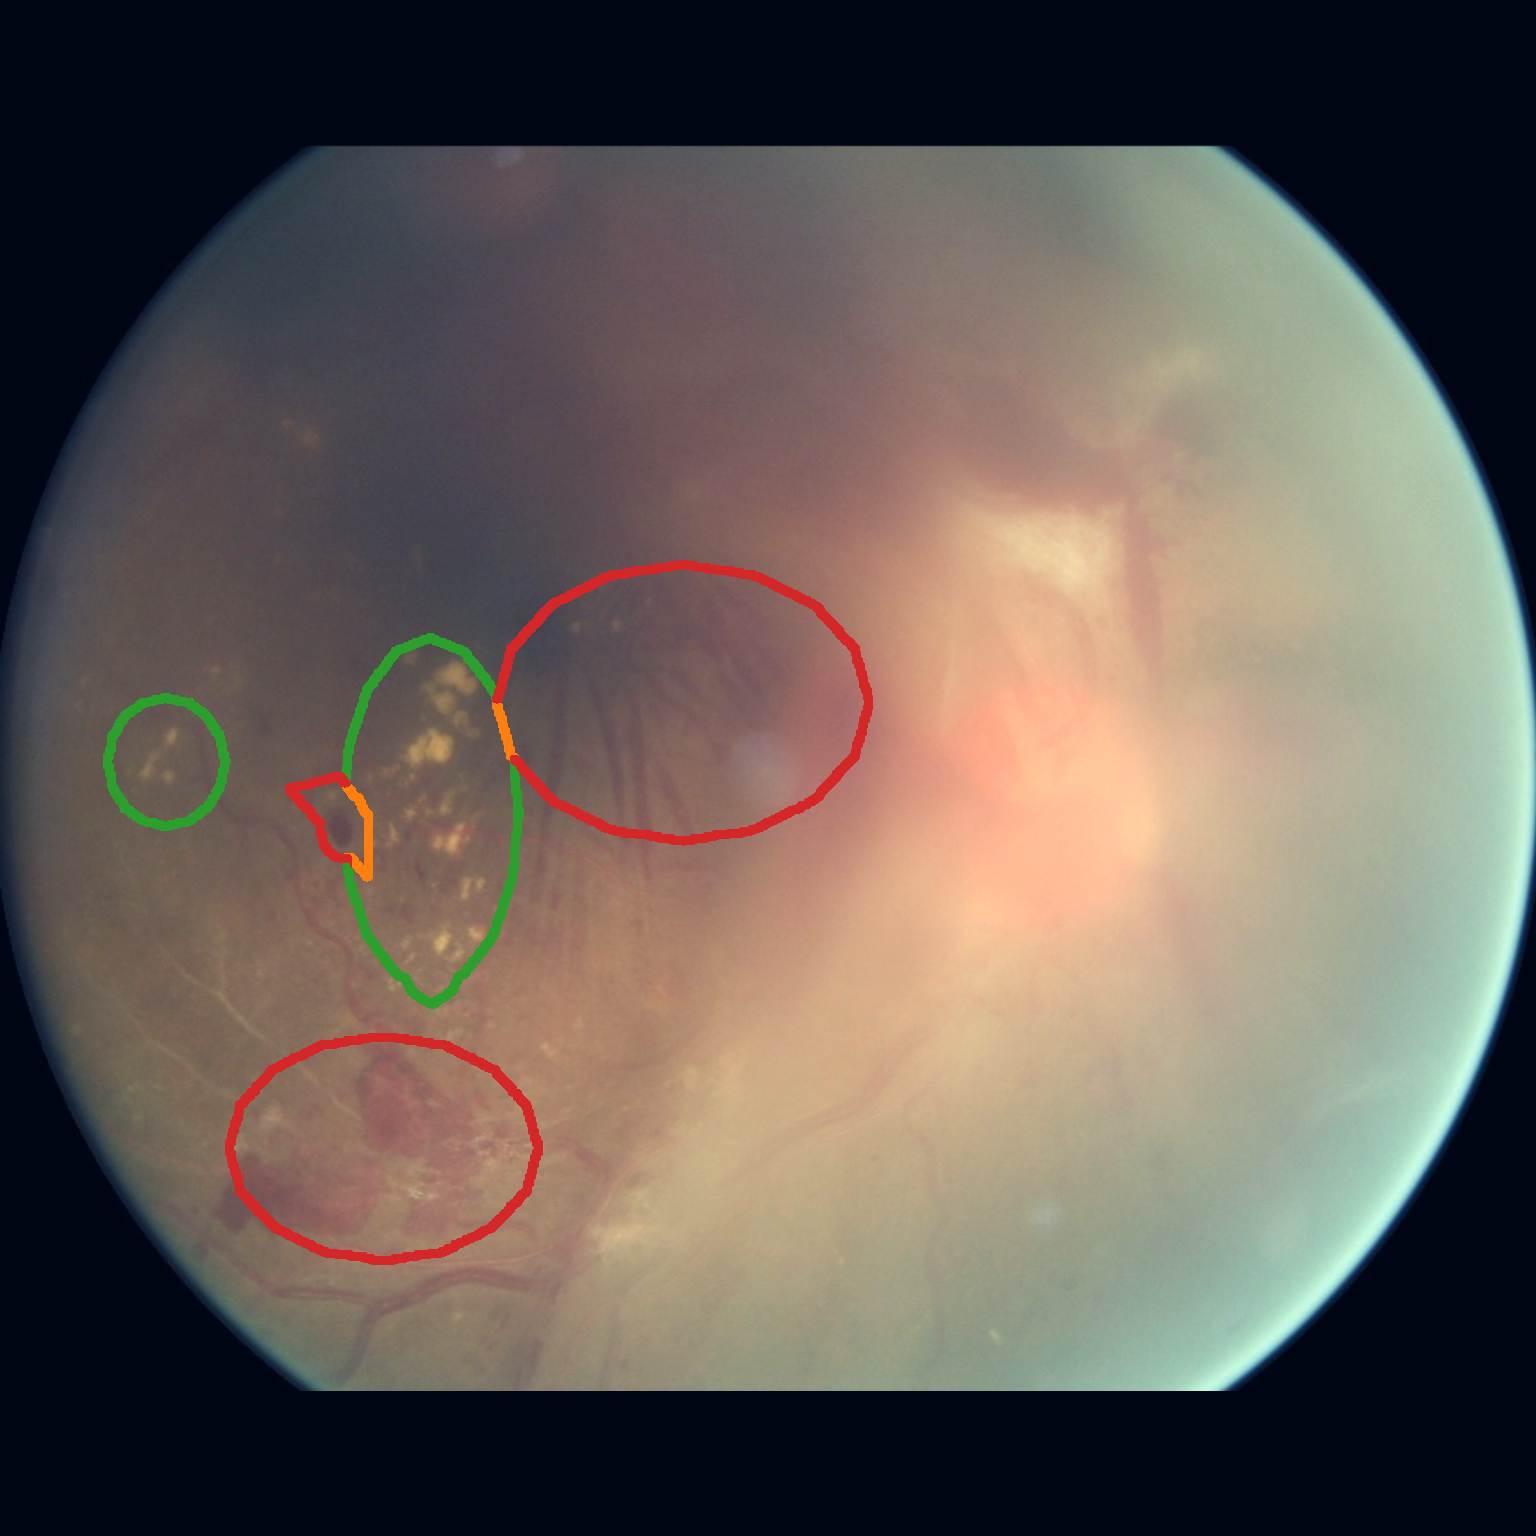
\includegraphics[width=\textwidth]{segmentation_lesions/difficultees/faible_contraste.png}
		\caption{Faible contraste dans le champ nasal due à une pathologie (détachement rétinien ou cataracte)}
	\end{subfigure}
\caption{Images issues de la base de données RET-LES.}
\label{fig:DifficultesAcquisition}
\end{figure}

Nous avons également eu l'occasion de vérifier cette difficulté liée à l'identification des lésions en conduisant également une micro-étude auprès de trois experts de la rétine. Nous leur avons demandé de faire la gradation de la rétinopathie diabétique sur 200 images ainsi que l'identification de la présence d'\oe dème maculaire, suivant une échelle classique de 0 à 4. Il en ressort notamment douze images (6\%), pour lesquelles il existe un désaccord total entre les trois observateurs (c'est-à-dire qu'aucune paire ne s'accorde). Après révisions une-à-une des images en session, le désaccord s'avéra porter sur l'identification de certaines structures en tant que lésions de type micro-anévrismes. Or, sur cinq des douze images, une poussière sur le capteur de la caméra, visible dans la région maculaire, a trompé deux des trois observateurs sur la présence d'un micro-anévrisme. Le dernier observateur a constaté la présence de cette anomalie en comparant la position (toujours identique) de ce faux anévrisme sur ces 5 images consécutivement.
\\ 
Cette anecdote témoigne du type de difficultés existant dans la segmentation rétinienne et du défi qu'elle représente y compris pour des experts humains.
\subsection{Variabilité inter-bases}
\label{sec:variabilitéSegmentation}
Les cinq bases de données que nous analysons font état d'importantes inter-disparités à deux niveaux:
\begin{itemize}
	\item En terme d'images en elles-mêmes; les facteurs de variabilité étant l'apparence de l'image (terme générique regroupant la colorimétrie, le contraste, l'exposition...), la résolution, la qualité d'acquisition et la diversité des symptômes des patients présents dans la base.
	\item En terme d'annotations réalisées par les médecins; cette fois, ce sont la finesse (c'est-à-dire la précision aux frontières) des annotations,  leur quantité et le nombre de classes différentes annotées qui font cette diversité.
\end{itemize}
Bien entendu, à cela s'ajoute que les bases de données sont de taille diverses. Le tableau \ref{tab:databasesCaracteristics} fournit le détail de la composition de chaque base.
\begin{table}
	\centering
	\caption{Composition de chacune des bases de données utilisées. \acf{HIV}, \acf{HIR}, \acf{HPR}, \acf{IrMA}, \acf{NV}}
	 \rowcolors{2}{white}{gray!10}
	\begin{tabularx}{\linewidth}{llcX}
		\toprule
		Bases & Nombre d'images & Résolution & Classes annotées \\
		\midrule
		\ac{IDRiD} & 81 & $2848 \times 4288$ & \ac{MA}, \ac{HEM}, \ac{CWS}, \ac{EX}\\
		MESSIDOR & 200 & $1500\times 1500$ & \ac{MA}, \ac{HEM}, \ac{CWS}, \ac{EX}, Drusen, Macula, Disque Optique, Coupe Optique, \ac{HPR}, \ac{NV}, Vaisseaux Sanguins\\		
		\ac{DDR} & 757 & $1934 \times 1956$ & \ac{MA}, \ac{HEM}, \ac{CWS}, \ac{EX}\\
		RET-LES & 1593 & $896 \times 896$ & \ac{MA}, \ac{HEM}, \ac{CWS}, \ac{EX}, \ac{NV}, \ac{HIV}, \ac{HIR}, Prolifération Fibreuse\\
		\ac{FGADR} & 1842 & $1280 \times 1280$ & \ac{MA}, \ac{HEM}, \ac{CWS}, \ac{EX}, NV, IRMA\\		
		\bottomrule
	\end{tabularx}

\label{tab:databasesCaracteristics}
\end{table}

La variabilité statistique des annotations dépend grandement du protocole d'annotation, sur lequel nous n'avons en général que peu d'informations. Or, la variabilité qu'il induit est très important: nous en proposons une estimation quantifiable sur la figure \ref{fig:annotationsManuellesBases}.
La finesse des annotations d'une base comme \ac{IDRiD} suggère une assistance par ordinateur pour faciliter un marquage extrêmement détaillé. Nous pouvons attester que cette stratégie est utilisée sur MESSIDOR, le processus d'annotations ayant été réalisé dans le cadre de ce doctorat en collaboration avec des cliniciens ayant vérifié et corrigé les annotations pré-réalisées automatiquement par un modèle.
Inversement, sur RET-LES, les annotations suggèrent un tracé à la main à partir de formes géométriques simples pré-définies. Entre ces deux extrêmes, les styles varient: comme on peut le voir sur la colonne correspondant à \ac{FGADR}, celle-ci présente à la fois des annotations aux frontières fines (trois premières lignes) et plus grossière (quatrième ligne).

\newcommand{\colSize}{0.19}
\begin{figure}
	\centering
	\begin{subfigure}{\colSize\textwidth}
		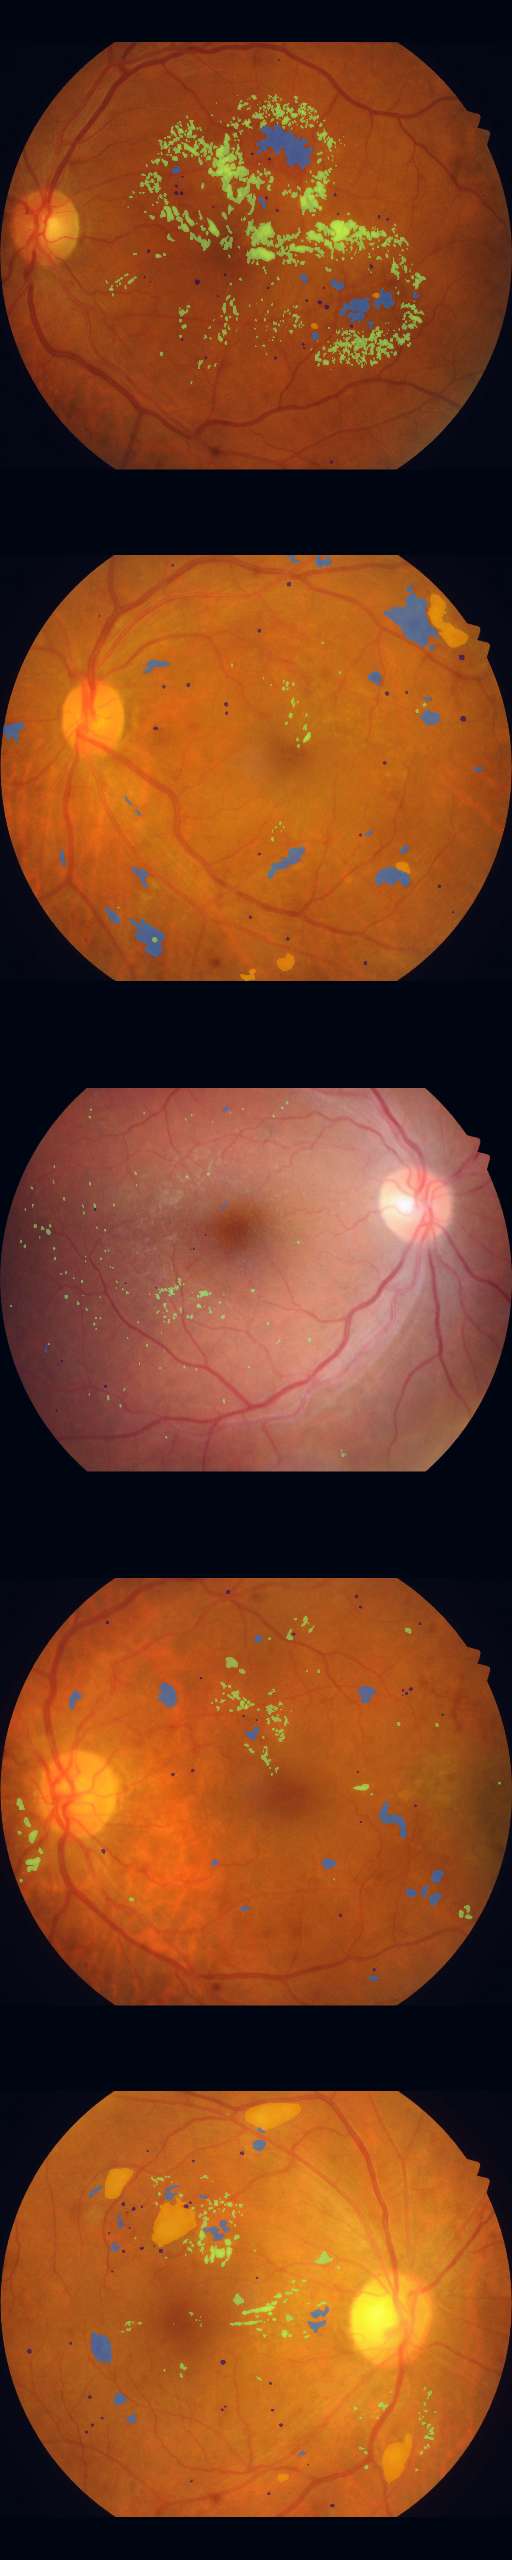
\includegraphics[width=\textwidth]{segmentation_lesions/distributions_labels/idrid.png}
		\caption{IDRID}
	\end{subfigure}
\begin{subfigure}{\colSize\textwidth}
	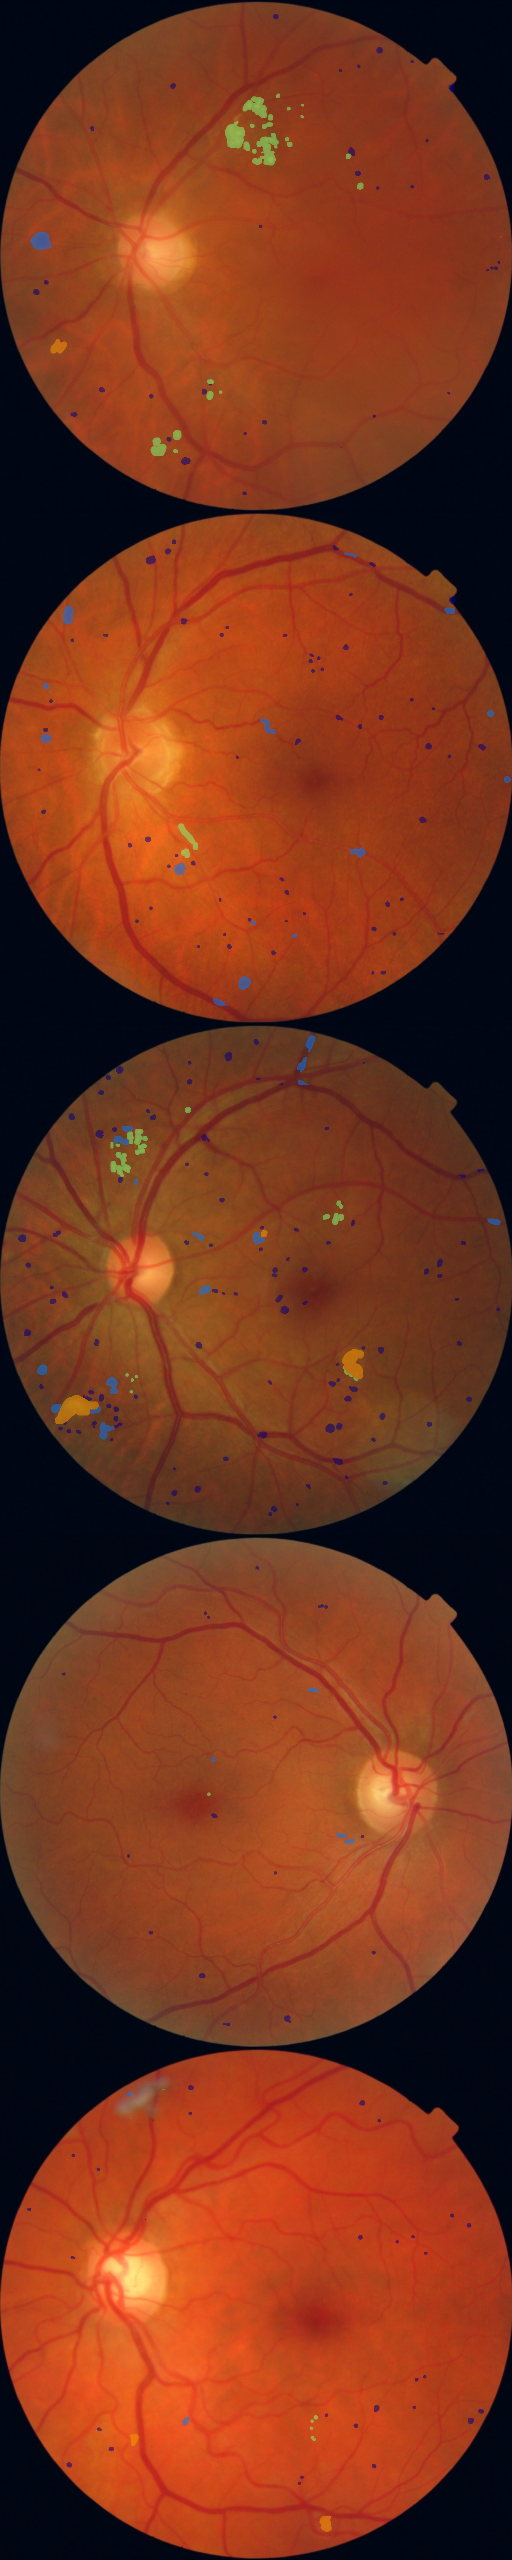
\includegraphics[width=\textwidth]{segmentation_lesions/distributions_labels/messidor.png}
	\caption{MESSIDOR}
\end{subfigure}
\begin{subfigure}{\colSize\textwidth}
	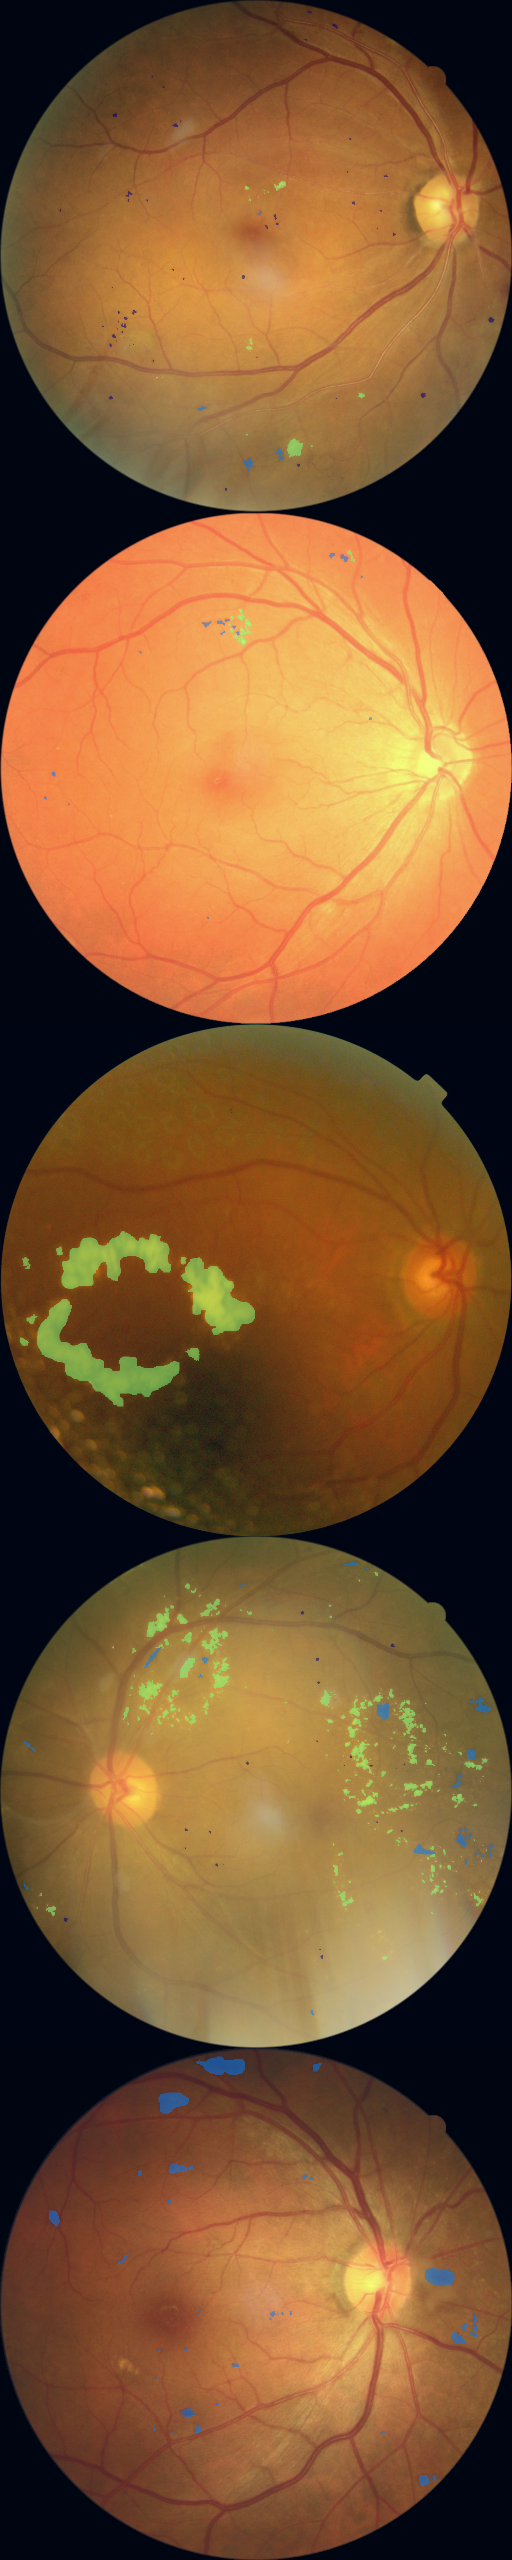
\includegraphics[width=\textwidth]{segmentation_lesions/distributions_labels/ddr.png}
	\caption{DDR}
\end{subfigure}
\begin{subfigure}{\colSize\textwidth}
	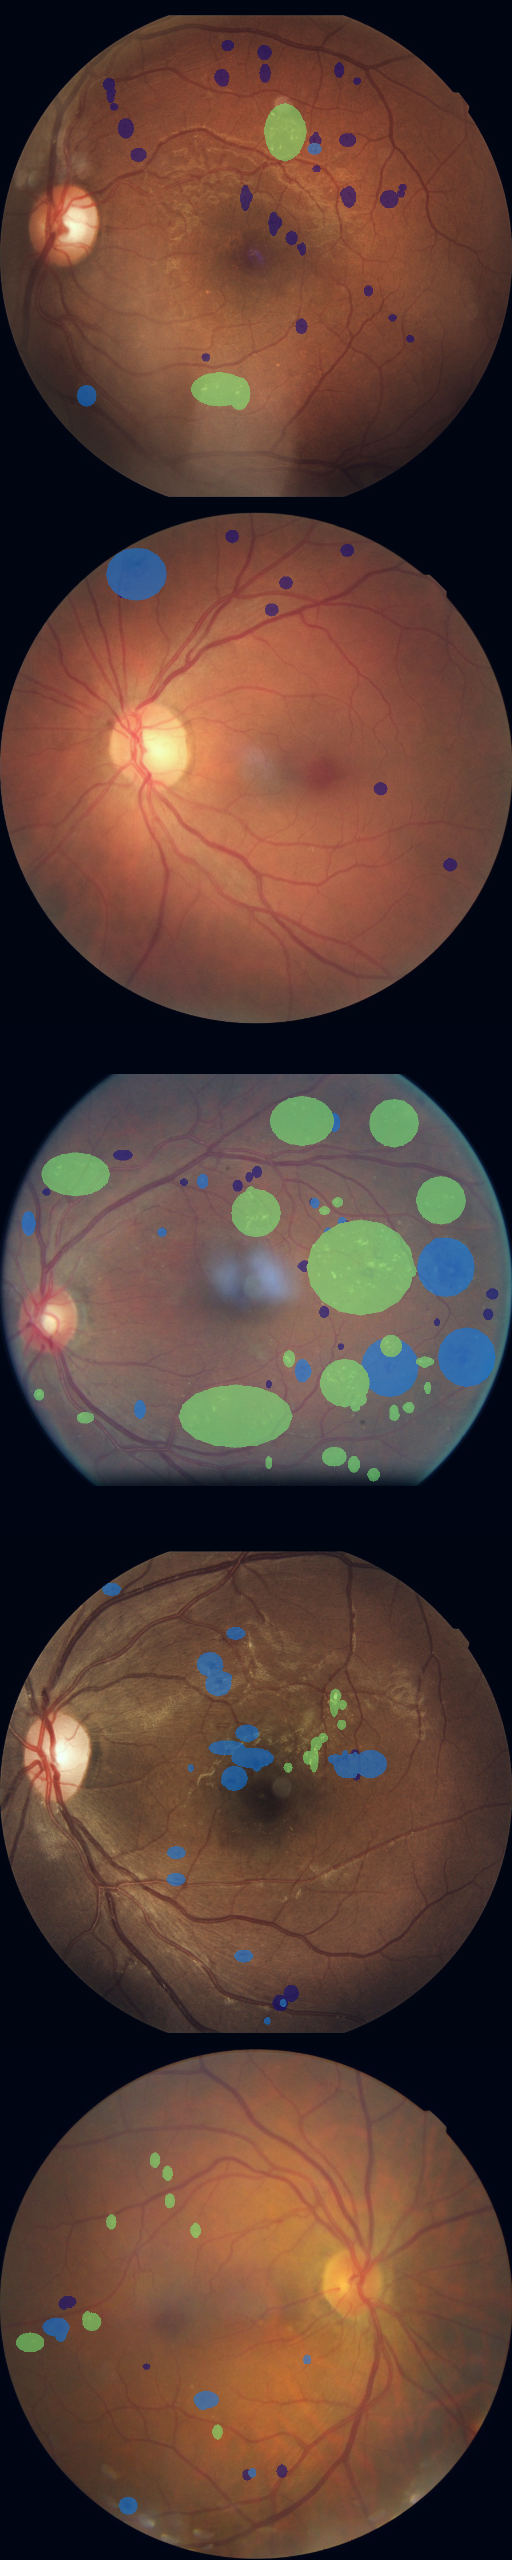
\includegraphics[width=\textwidth]{segmentation_lesions/distributions_labels/RETINAL_LESIONS.png}
	\caption{RET-LES}
\end{subfigure}
\begin{subfigure}{\colSize\textwidth}
	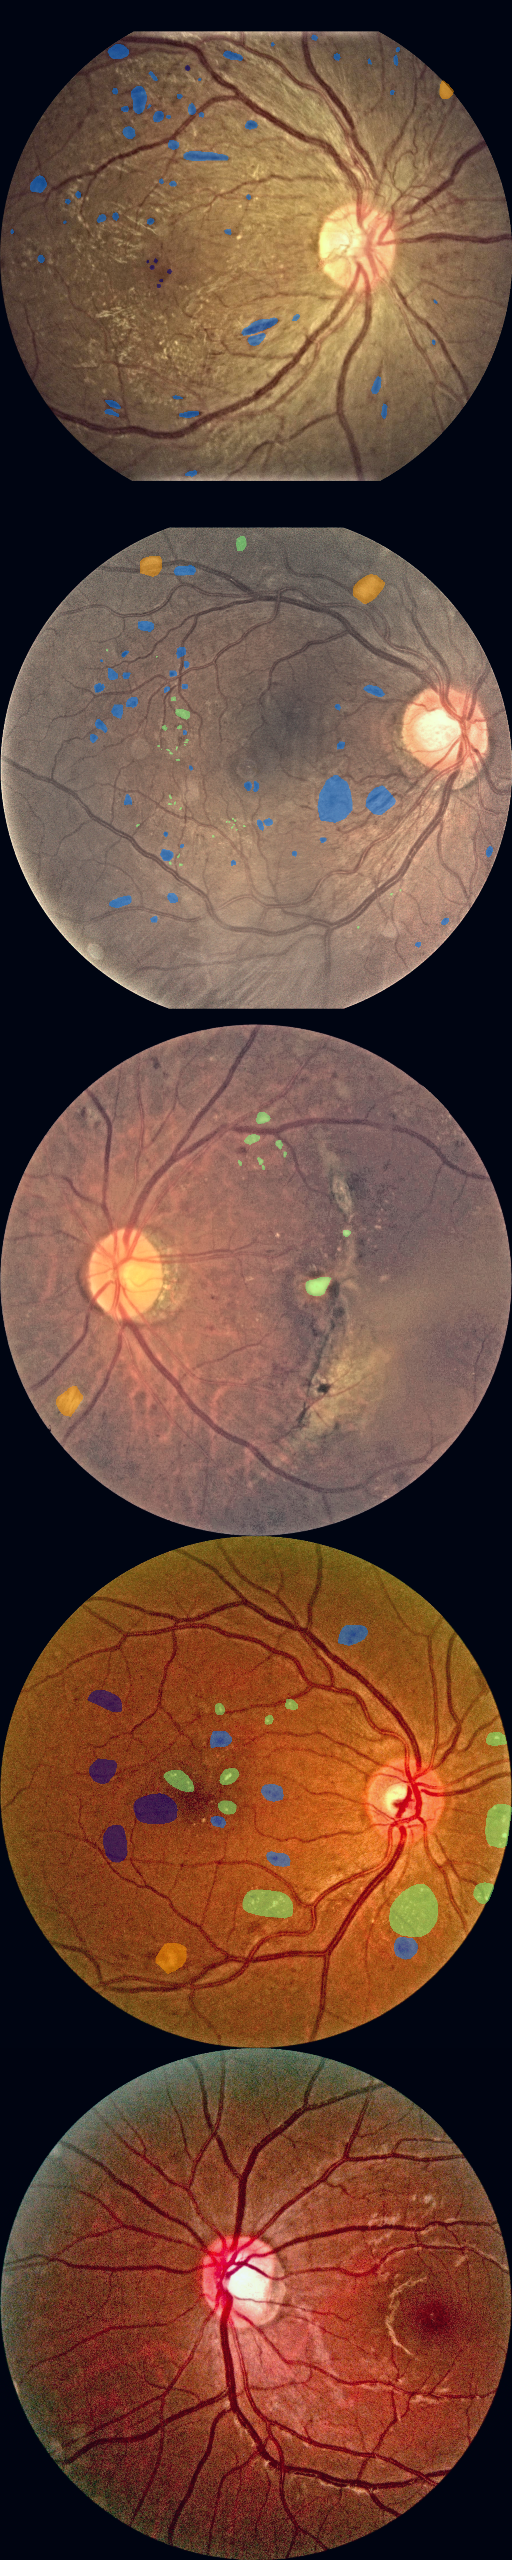
\includegraphics[width=\textwidth]{segmentation_lesions/distributions_labels/fgadr.png}
	\caption{FGADR}
\end{subfigure}
\caption{Images accompagnées de leurs annotations manuelles organisées suivant leur base d'appartenance. Que ce soit dans les couleurs, le découpage de la région d'intérêt ou les annotations, on constate une grande variabilité inter et intra base.}
\label{fig:annotationsManuellesBases}
\end{figure}
Il est possible de se faire une idée plus quantifiée du style d'annotations propre à chaque base. Pour cela, on propose une analyse statistique de la distribution jointe du nombre de lésions et de leur taille moyenne par image. Bien entendu, ces deux variables dépendent du diagnostic de la maladie sous-jacente, mais ici toutes les images considérées sont pathologiques (à des degrés de sévérité divers). Abstraction donc faite de la maladie, la seconde dépendance entre ces variables vient du style d'annotation. En particulier, deux régimes se distinguent: pour une annotation de granularité fine, l'expert aura tendance à marquer de nombreux éléments de manière précise et détaillée. Inversement, une annotation plus grossière aura tendance à fusionner ensemble les structures locales voisines en des structures plus grosses et moins nombreuses. La figure \ref{fig:jointDistributionLesion} montre ces distributions jointes pour les quatre lésions et pour chacune des cinq bases de données. Elle met bien en évidence l'observation qualitative: \ac{IDRiD} se distingue par un grand nombre d'éléments segmentés de petite taille, suivi généralement de \ac{DDR} et MESSIDOR. RET-LES est systématiquement la moins fine, toutes lésions confondues (celles-ci étant moins nombreuses et de plus grande taille). Enfin, tel que visible sur la figure \ref{fig:annotationsManuellesBases}, FGADR se retrouve à cheval entre ces deux tendances, présentant des images possédant de nombreuses lésions de petites tailles et d'autres en possédant peu mais de grandes tailles. 

\begin{figure}
	\begin{subfigure}{.5\textwidth}
		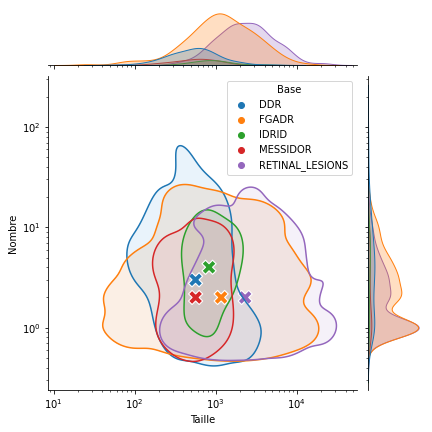
\includegraphics[width=\textwidth]{segmentation_lesions/distributions_labels/Cotton_Wool_Spot.png}
		\caption{Distribution des \ac{CWS}}
	\end{subfigure}
	\begin{subfigure}{.5\textwidth}
		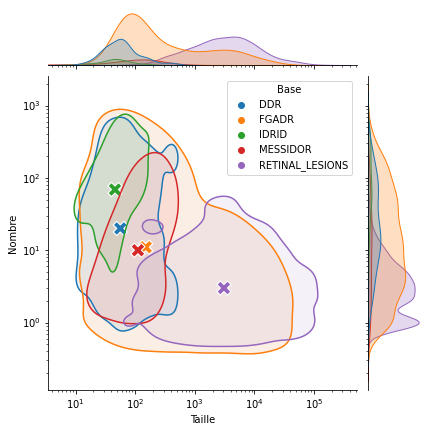
\includegraphics[width=\textwidth]{segmentation_lesions/distributions_labels/Exudates.png}
		\caption{Distribution des \ac{EX}}
	\end{subfigure}
	\begin{subfigure}{.5\textwidth}
		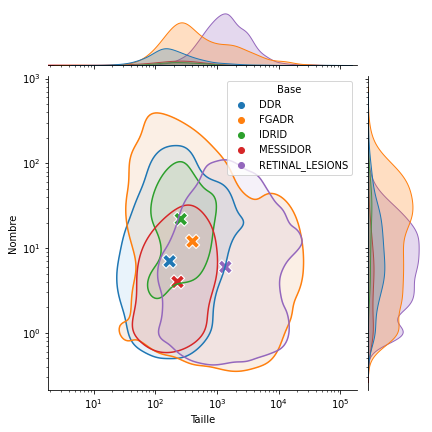
\includegraphics[width=\textwidth]{segmentation_lesions/distributions_labels/Hemorrhages.png}
		\caption{Distribution des \ac{HEM}}
	\end{subfigure}
	\begin{subfigure}{.5\textwidth}
		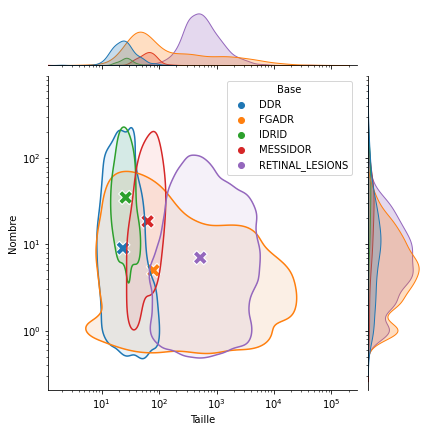
\includegraphics[width=\textwidth]{segmentation_lesions/distributions_labels/Microaneurysms.png}
		\caption{Distribution des \ac{MA}}
	\end{subfigure}
\caption{Représentation des distributions jointes de la taille moyenne et du nombre de lésions par images pour chaque classe. Les croix représentent les centroïdes de chaque distribution. Pour pouvoir représenter les distributions sur un même graphique, il a fallu choisir une échelle logarithmique, il y a donc plusieurs ordres de grandeur séparant les centroïdes.  En comparant les bases de données, on met ainsi en évidence la disparité des styles d'annotations entre chacune.}
\label{fig:jointDistributionLesion}
\end{figure}


\section{Problématique}
\label{sec:SegmentationProblematique}
Considérant les éléments relatifs aux deux sections précédentes (c'est-à-dire les difficultés liées à la segmentation et la grande variabilité inter-base existante), plusieurs éléments de problématique se posent: 
\begin{itemize}
	\item Quelles sont les capacités de généralisation d'un modèle donné sur diverses bases de données?
	\item Corollairement, que peut-on conclure des performances d'un modèle à partir d'une seule base?
	\item Quel impact le style d'annotations propre à chaque base va-t-il avoir sur le diagnostic de la pathologie?
\end{itemize}
À travers les deux premières questions, nous dressons un premier objectif de recherche, qui est de concevoir un modèle capable de segmenter plusieurs lésions simultanément. Nous ajoutons deux contraintes techniques sur le choix du modèle: celui-ci doit pouvoir être facilement reproductible (donc sans ambiguïté d'implémentation) et ses performances doivent a minima égaler les modèles de l'état de l'art. Ce modèle nous servira de base pour évaluer les problématiques de généralisation.
\\
Notre second objectif de recherche porte sur l'évaluation de la capacité de généralisation empirique du modèle sur différentes bases afin de dresser le tableau des compatibilités inter-bases. \\
Une question de recherche vient se greffer à cet objectif, qui est celle de la pertinence des métriques utilisées pour l'évaluation de la qualité de la segmentation. Pour répondre à ce questionnement, un autre axe d'analyse sera traité, qui décrit la relation entre qualité de la segmentation et de détection des lésions. 
\\
En vue d'uniformiser les performances inter-bases, il est assez intuitif de vouloir réduire la variabilité entre les images présentées par un effet de prétraitement. Nous proposons d'explorer l'effet qu'induit un tel type de traitement sur le modèle.
\\
Nous nous attendons à trouver des disparités au sein des modèles de segmentation dépendamment de leur base d'entraînement. Notre objectif principal est à la fois d'en étudier les conséquences en terme de segmentation sur des images de test mais aussi de proposer une méthode pour contrôler le comportement des modèles en fonction du besoin clinique. On notera cependant que celui-ci n'est pas clairement défini:
dans quelle mesure ces disparités de segmentation sont-elles cliniquement pertinentes ou dommageables? \\
Pour clarifier cette question, nous proposons dans un dernier temps d'étudier la capacité d'un modèle à classifier une image à partir des lésions identifiées en elle. 

\section{Méthodologie}
Notre méthodologie s'articule autours de quatre axes, dont chacun fait l'objet d'une section dans la partie qui suit:
\begin{enumerate}
	\item La standardisation via des traitements algorithmiques simples des images d'entrée.
	\item La conception d'une architecture de segmentation, incluant sa comparaison avec l´état de l'art.
	\item La mise en place d'une stratégie permettant d'uniformiser les performances d'un modèle à travers plusieurs distributions de données.
	\item Le développement d'un modèle de classification permettant l'évaluation de la pertinence de la segmentation à des fins diagnostiques.
\end{enumerate}
\subsection{Normalisation des données}
Les images utilisées varient en résolution et en apparence. La phase de prétraitement vise donc à corriger ces deux aspects et est présentée dans cette section. La standardisation des résolutions est une nécessité technique, notamment du fait que les modèles ne sont théoriquement pas invariants en échelle; elle est donc menée pour chacune de nos expériences. En revanche, l'intérêt de l'homogénéisation de l'apparence est plus discutable. Pour alléger ce chapitre et à la vue de résultats mitigés, nous le mentionnons brièvement dans la section \ref{sec:preprocessingQuick} mais le détail des résultats est reporté en annexe \ref{an:PrétraitementDonnées}.
\subsubsection{Standardisation des résolutions}
\label{sec:resolution_standardisation}
La résolution d'image varie dépendamment de la base. Afin de standardiser le format d'entrée de nos modèles, notre protocole inclut les étapes suivantes:
\begin{enumerate}
	\item La région d'intérêt (rétine) est extraite. Pour cela, on utilise un simple effet de seuillage sur le canal rouge de l'image.
	\item L'image est ensuite découpée pour éliminer les bordures noires et ainsi être centrées sur la région d'intérêt.
	\item Si l'image résultante n'est pas de format carrée, on utilise du \textit{padding} (complétion des bords par des zéros) sur la dimension la plus petite pour lui conférer ce format.
	\item L'image est ensuite redimensionnée au standard que nous avons adopté de $1536 \times 1536$.
\end{enumerate}
On peut noter que cette résolution est supérieure à celle des images fournies dans RET-LES et FGADR. Pour ces deux bases, les images apparaîtront comme légèrement moins détaillées (la sous-résolution initiale pouvant agir comme un filtre passe-bas). En pratique, nous avons quantifié cet effet, en utilisant des images de très hautes résolutions (type IDRID), filtrées par un passe-bas pour simuler une sous-résolution. Nous n'avons pas observé de changements drastiques de comportement des CNNs entraînés dépendamment de ce filtrage, ce qui semble légitimer la sur-résolution de toutes les bases au standard que nous avons adopté. Précisons tout de même que la résolution choisie reste exceptionnellement élevée: dans la littérature, la plupart des modèles sont entraînés sur des images de taille $512 \times 512$. Plusieurs travaux font cependant état d'une corrélation entre qualité du dépistage et résolution des images, il paraît donc pertinent d'adopter un standard élevé pour celle-ci.
\subsubsection{Algorithme de prétraitement}
\label{sec:preprocessingQuick}
La nécessité et l'impact d'un prétraitement des données -visant à homogénéiser l'apparence des images indépendamment de leur origine- sont encore très débattus dans la littérature. Nous avons mené nos propres expériences en la matière. Le protocole et les résultats détaillés sont fournis en annexe \ref{an:PrétraitementDonnées} mais en voici les conclusions résumées:  quel que soit l'angle d'analyse choisi (par lésions ou par bases de données), les gains potentiels obtenus par un traitement visant à normaliser l'apparence des images semblent limités. En revanche, il existe des cas pour lesquels ils entraînent des situations de faillite complète de convergence du modèle mais nous n'avons pas exploré les raisons expliquant ces configurations défectueuses. Pour la suite du chapitre, nous considérons donc les images dans leur apparence initiale, sans algorithme de prétraitement.

\subsection{Conception d'une architecture polyvalente}
\label{sec:segConceptionArchitecture}
Le choix d'une architecture de réseau de neurones est sujet à de nombreuses considérations sur les données et le budget calculatoire disponible. De nombreux travaux sur la segmentation du \fundus{} mettent en avant (voir la revue de littérature en section \ref{sec:segmentationFCCN}) la grande variabilité de taille des lésions et proposent des modèles combinant une approche locale et globale pour la prendre en compte. Mais en pratique, notre revue de littérature ne fait pas ressortir une architecture indiscutablement plus performante que les autres, trop de variables (nombre de paramètres, résolution d'images, prétraitement, itérations d'entraînement) étant interdépendantes sans qu'il n'y ait de consensus sur leur importance respective. De plus, les variations de performances sont souvent relativement minimes, qui plus est sur des métriques bien précises et potentiellement sensibles à des micro-variations (par exemple dues aux frontières de segmentation, par nature ambiguës). On observe également souvent une absence de standard dans le rapport fourni des résultats, que ce soit sur le choix de la métrique ou son mode de calcul. Heureusement, des concours comme \ac{IDRiD} ont permis de corriger cet aspect dans une certaine mesure, standardisant l'utilisation de certaines métriques et facilitant ainsi les comparaisons. Enfin, pour l'essentiel de la littérature, on note que seules les performances de segmentation sont rapportées et non celles de détection. Or, aucun travail ne semble s'interroger sur la pertinence d'une segmentation fine d'un point de vue diagnostic par rapport à une simple détection: autrement dit, la précision sur les frontières de segmentation n'a, pour l'heure, pas démontré sa pertinence clinique. 
\\
En dressant cet inventaire des freins à la comparaison à l'état de l'art, on dessine en creux une critique d'une tendance assez fréquente: celle de voir apparaître de nouvelles architectures introduites sans prendre en compte l'existant et la modularité des réseaux de neurones existants. Nous arguons qu'en l'absence de consensus sur ce qui fait la performance pratique d'un modèle, il est relativement superflu de se concentrer sur la construction de nouvelles architectures spécifiques au \fundus.
\\
Au contraire, nous suggérons d'utiliser la modularité des réseaux de neurones, qui nous permet d'obtenir une pléthore de combinaisons parmi les architectures existantes. Ces modèles ont l'avantage d'avoir été largement étudiés et éprouvés dans la littérature sur des bases de données généralistes autrement plus grandes et diverses. Par ailleurs, ces modèles sont plus facilement reproductibles, y compris dans leur version pré-entraînée car nous les avons extraits de librairies publiques connues.
 \\
Pour appuyer notre propos et afin de sélectionner l'architecture qui nous servira à conduire notre étude de généralisation, nous proposons d'explorer les forces de cette modularité architecturale, en combinant différent blocs. Toutes les architectures testées fonctionnent sur un même modèle de type:
\begin{equation}
	y = \mathcal{D}(\mathcal{E}(x))
\end{equation}
où $x, y$ sont respectivement les entrées et les sorties du modèle, $\mathcal{E}$ représente un module d'encodage et $\mathcal{D}$ de décodage. L'encodeur produit une ou plusieurs cartes de caractéristiques à différentes résolutions et le décodeur a la tâche de les combiner en une unique carte de segmentation. À partir de cette description simple, nous pouvons piocher dans la littérature pour concevoir séparément nos modules d'encodage et de décodage en respectant des structures d'architectures existantes. Le tableau \ref{tab:segmentationNetworks} reporte l'ensemble des combinaisons essayées. Le fonctionnement des différents modules sont décrits dans la section \ref{sec:FCCN}. Certains modules ne sont pas compatibles entre eux (ce qui explique les cases vides du tableau). En considérant ceux-ci, on aboutit à un total de 27 architectures comparées.
Cela nous permet de couvrir une large gamme de modèles, à la taille et à la complexité très variables. Notons que tous les modèles ne sont pas convolutifs, en particulier, les encodeurs MIT B2/4 se basent sur l'architecture du SegFormer (utilisant des réseaux auto-attentifs).

\begin{table}
	\centering
	\caption{Architectures utilisées dans notre étude comparative, accompagnées de leur taille (paramètres et FLOPs)}
	\label{tab:segmentationNetworks}
	\begin{tabularx}{\textwidth}{Xlcc}
		\toprule
		Architecture & Encodeur & \# Paramètres & \# FLOPs \\
		\midrule
		\multirow{8}{3em}{UNet} & ResNet 18  & 14.33M & 21.82G \\ 
		& ResNet 34  & 24.44M & 31.49G \\ 
		& SE ResNet50  & 35.05M & 41.67G \\ 
		& ResNest - 50  & 34.45M & 49.57G \\ 
		& EfficientNet-B7  & 67.1M & 39.2G \\ 
		& MobileNetV3  & 3.59M & 10.43G \\ 
		& MIT B2  & 27.48M & 31.6G \\ 
		& MIT B4  & 64.12M & 64.92G \\ 
		\midrule
		\multirow{8}{3em}{UNet++} & ResNet 18  & 15.97M & 64.18G \\ 
		& ResNet 34  & 26.08M & 73.85G \\ 
		& SE ResNet50  & 51.52M & 0.23T \\ 
		& ResNest - 50  & 50.91M & 0.24T \\ 
		& EfficientNet-B7  & 68.16M & 75.32G \\ 
		& MobileNetV3  & 3.71M & 13.97G \\ 
		& MIT B2  & \multicolumn{1}{c}{-} & \multicolumn{1}{c}{-} \\ 
		& MIT B4  & \multicolumn{1}{c}{-} & \multicolumn{1}{c}{-} \\ 
		\midrule
		\multirow{8}{3em}{FPN} & ResNet 18  & 13.05M & 17.85G \\ 
		& ResNet 34  & 23.16M & 27.53G \\ 
		& SE ResNet50  & 28.65M & 30.15G \\ 
		& ResNest - 50  & 28.04M & 38.05G \\ 
		& EfficientNet-B7  & 65.67M & 35.27G \\ 
		& MobileNetV3  & 2.72M & 8.29G \\ 
		& MIT B2  & 26.08M & 28.7G \\ 
		& MIT B4  & 62.73M & 62.03G \\ 
		\midrule
		\multirow{8}{3em}{DeepLab V3+} & ResNet 18  & 12.33M & 18.33G \\ 
		& ResNet 34  & 22.44M & 31.63G \\ 
		& SE ResNet50  & 29.21M & 35.97G \\ 
		& ResNest - 50  & \multicolumn{1}{c}{-} & \multicolumn{1}{c}{-} \\ 
		& EfficientNet-B7  & 65.11M & 60.21G \\ 
		& MobileNetV3  & 2.16M & 2.98G \\ 
		& MIT B2  & \multicolumn{1}{c}{-} & \multicolumn{1}{c}{-} \\ 
		& MIT B4  & \multicolumn{1}{c}{-} & \multicolumn{1}{c}{-} \\ 
		\bottomrule
	\end{tabularx}
\end{table}



\subsection{Gradation automatique de la rétinopathie diabétique assistée par segmentation}
La dernière étape méthodologique de ce travail prend du recul sur la question de la qualité de la segmentation et interroge la pertinence de celle-ci dans un contexte clinique. Elle vise à répondre de manière plus pragmatique sur la qualité des segmentation produites par les différents modèles, cette fois non pas sous le prisme des performances pixel par pixel, mais sous l'angle de la pertinence de celles-ci pour le diagnostic de l'image globale. Nous avons fait pour cela le choix d'une approche par graphe pour classifier une image de \fundus{} en différents grades de maladie (la rétinopathie diabétique) à partir de ses lésions. Une telle approche est une contribution originale sans équivalents dans la littérature à notre connaissance. Pour la justifier, la section suivante \ref{sec:preliminaryExperimentClassSegm} est une parenthèse dans la description de notre méthodologie et présente les expériences préliminaires qui ont motivées l'approche par graphe. 

\subsubsection{Expériences préliminaires: le problème de la classification assistée par segmentation}
\label{sec:preliminaryExperimentClassSegm}
Il n'existe pas de façons univoques de labelliser les lésions dans une image, ce qu'atteste la variabilité des annotations selon les bases. Dans ce contexte, comment évaluer la qualité d'un modèle entraîné sur ces bases? Nous proposons de répondre à cette question par procuration en reformulant le problème:
étant donnée une carte de segmentation générée par un modèle, peut-on retrouver le diagnostic de l'image associée? Corollairement, quel style d'annotations est le plus efficace pour aboutir à un diagnostic? 
\\
Surprenamment, cette question est rarement posée dans la littérature. Certains travaux combinent l'étape de segmentation à celle de classification \cite{liDiagnosticAssessmentDeep2019b, zhouBenchmarkStudyingDiabetic2021, weiLearnSegmentRetinal2021a} et démontrent généralement des performances améliorées par l'ajout de cette combinaison. Mais dans le détail, il s'agit en général de gains relativement marginaux. Il est par ailleurs établi que les réseaux de neurones sont particulièrement doués pour classifier des images sans pré-segmentation. Ainsi, l'ajout des marqueurs segmentés peut être simplement vu comme une forme de guidage de l'apprentissage, comme une supervision renforcée par la distillation de l'expertise du modèle de segmentation. Mais aucuns de ces travaux n'étudient l'impact de la qualité des segmentations sur la classification, autrement dit, il n'y est pas du tout évident qu'une mauvaise segmentation entraînera une mauvaise classification. \\
Pour y voir plus clair, nous avons mené des expériences préliminaires, en combinant simplement un réseau de classification et de segmentation suivant différentes approches, librement inspirées par la littérature. Trois combinaisons sont expérimentées, représentées sur la figure \ref{fig:segClassModel}:
\begin{enumerate}
	\item Combinaison séquentielle: la sortie du réseau de segmentation est concaténée à l'image originale. Les cartes de segmentations résultantes sont fournies directement à un réseau de classification après concaténation avec l'image origine (ou sans dans la version alternative du modèle).
	\item Combinaison parallèle: les réseaux de segmentation et de classification reçoivent chacun la même image. Les caractéristiques issues de l'avant dernière couche de chaque encodeur sont concaténées.
	\item Combinaison hybride: ce scénario consiste en un mixte des deux précédents scénarios.
\end{enumerate}
Précision pratique: l'architecture de classification fonctionne sur une résolution d'image de $512 \times 512$ (contre $1536 \times 1536$ pour la segmentation). Pour pallier à cette différence, les cartes issues du réseau de segmentation sont interpolées à la résolution adéquate avant concaténation.
\begin{figure}
	\centering
	\begin{subfigure}{.7\textwidth}
		\centering
		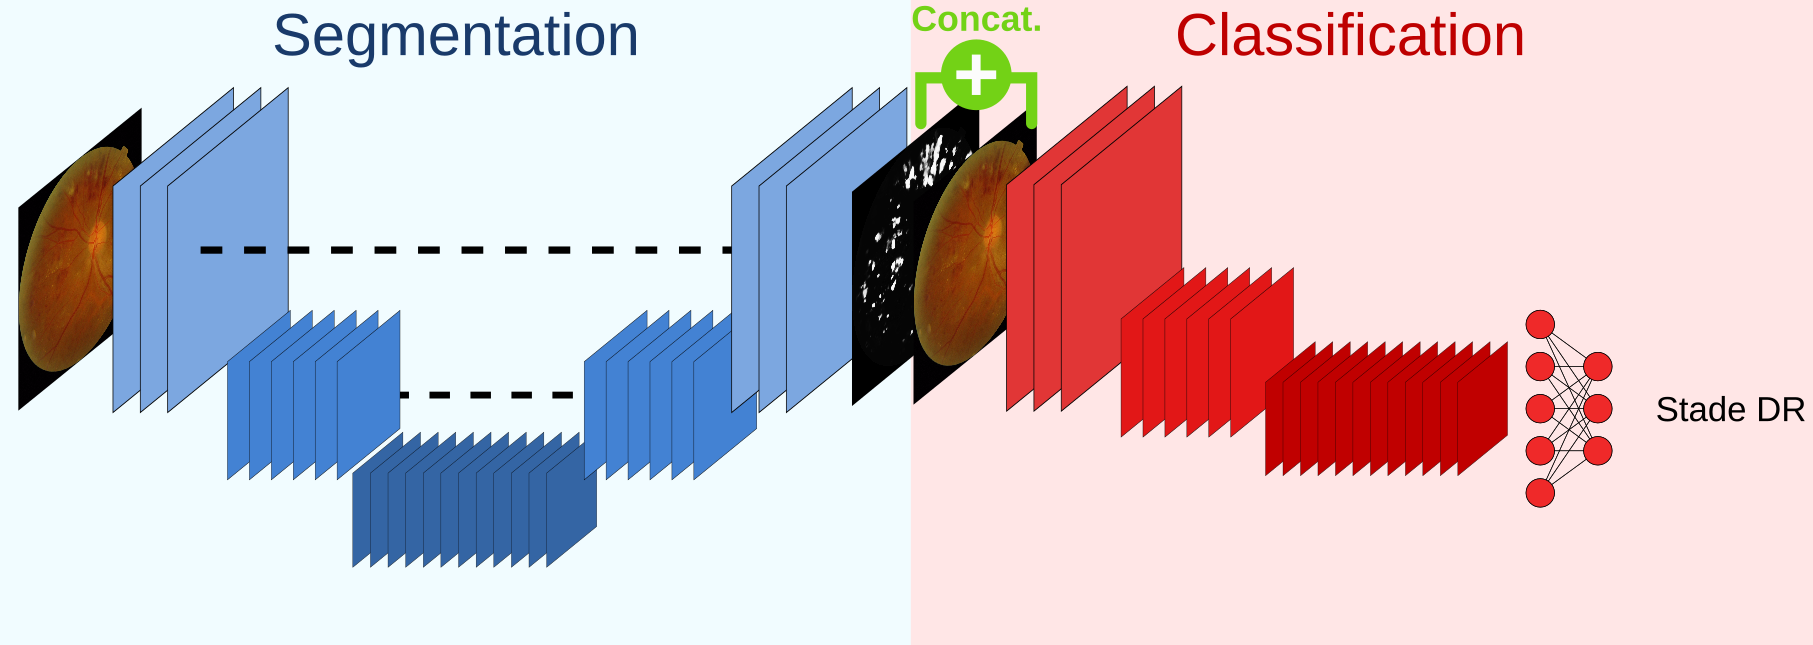
\includegraphics[width=\linewidth]{gnuplot/segmentation_lesions/gradation_dr/modele_serie}
		\caption{Réseaux de segmentation et classification mis en série. La sortie de la segmentation est envoyée comme entrée (concaténée à l'image) du réseau de classification}
	\label{fig:modeleserie}
	\end{subfigure}
	
	\begin{subfigure}{.7\textwidth}
		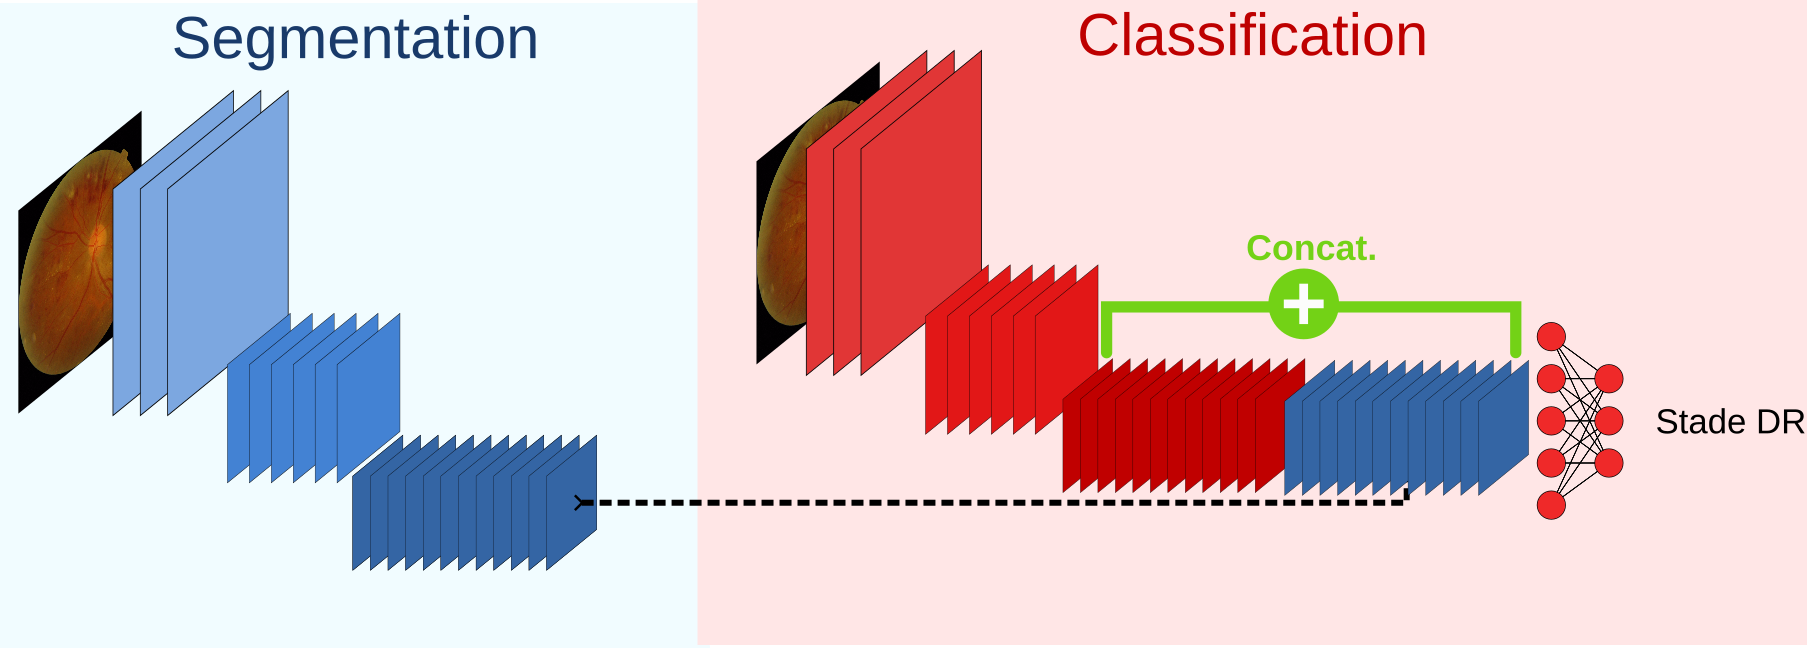
\includegraphics[width=\linewidth]{gnuplot/segmentation_lesions/gradation_dr/modele_parallele}
		\caption{Réseaux de segmentation et classification mis en parallèle, avec fusion des caractéristiques intermédiaires des deux modèles}
		\label{fig:modeleparalelle}
	\end{subfigure}
\begin{subfigure}{.7\textwidth}
	\centering
	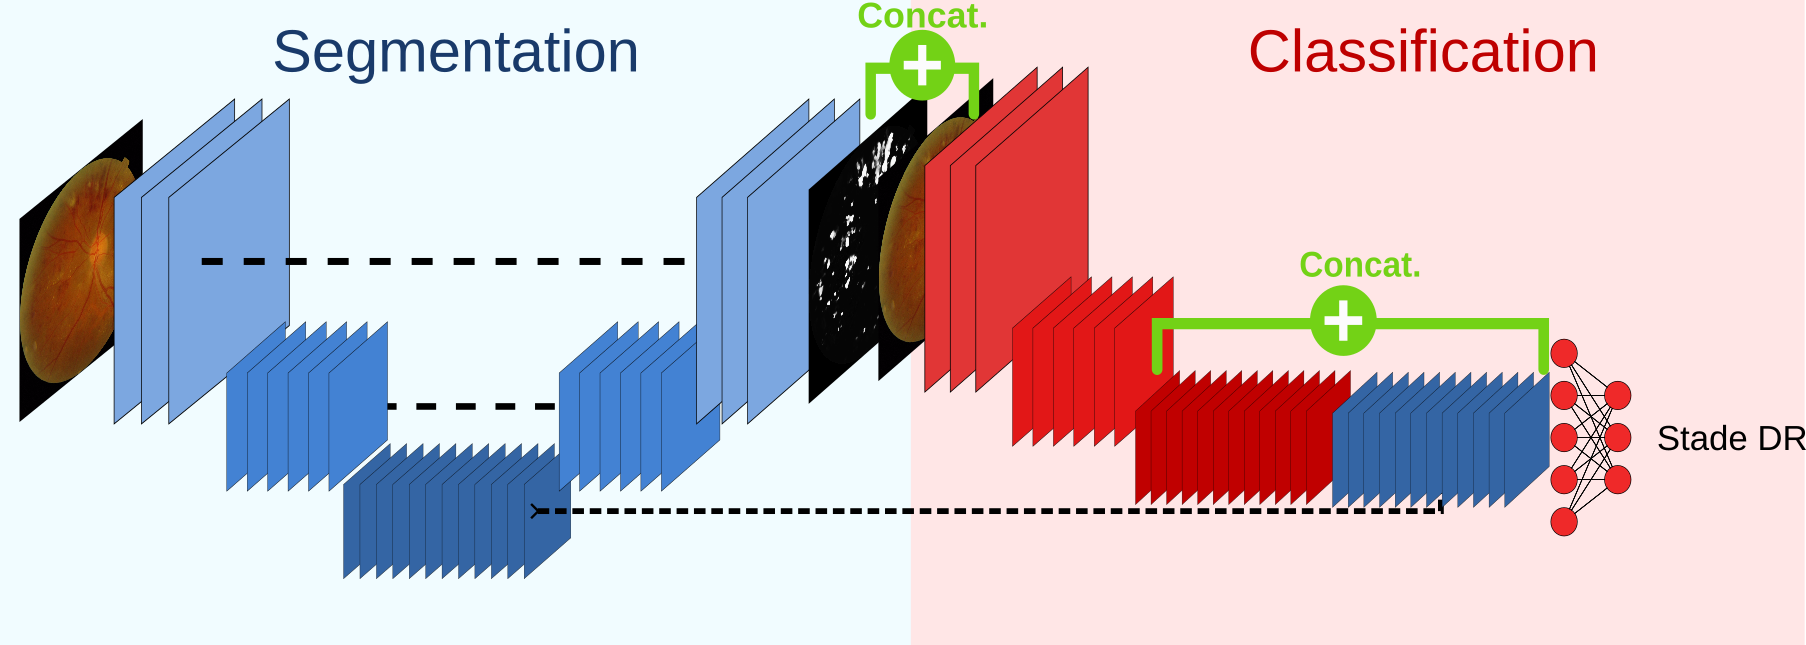
\includegraphics[width=\linewidth]{gnuplot/segmentation_lesions/gradation_dr/modele_combine}
	\caption{Combinaison parallèle/série, c'est-à-dire un mixte des approches \ref{fig:modeleserie} et \ref{fig:modeleparalelle}.}
	\label{fig:modelecombine}
\end{subfigure}
\caption{Dans le cadre d'une étude préliminaire sur la combinaison des informations de segmentation et de classification. Trois approches ont été expérimentées, basées sur différentes stratégies de combinaisons des deux réseaux}
\label{fig:segClassModel}
\end{figure}
Le modèle de segmentation est entraîné séparément, nous reviendrons dessus largement dans les sections qui suivent. Pour cette section, nous admettons disposer de différents modèles de segmentation fournissant des prédictions distinctes.
En entraînant la classification sur des jeux de données dédiés, nous avons mesuré la performance du modèle en utilisant le coefficient quadratique $\kappa$ de Cohen. Les bases de données utilisées sont EyePACS  \cite{cuadros_bresnick_2009} (divisée en ensembles d'apprentissage et de test) et APTOS \cite{APTOS2019Blindness2019} (test uniquement). Ces données, que nous ré-employons dans le chapitre suivant, y seront décrites avec plus de détails (en particulier dans la section \ref{sec:databaseFocusedAttention}). Précisons simplement que ces bases, bien plus conséquentes que celles-dédiées à la segmentation, fournissent des images et un grade de rétinopathie diabétique suivant une échelle allant de 0 à 4. Les résultats obtenus avec nos différentes combinaisons sont présentés dans le tableau \ref{tab:PerfModelClassifSegmen}. À l'inverse de plusieurs tendances de littérature, il y apparaît que l'ajout d'une segmentation n'améliore pas systématiquement les performances de classification. On obtient cependant des combinaisons pour lesquelles celles-ci sont rehaussées par l'intégration du modèle de segmentation.
Il est donc possible que seules certaines symbioses classification-segmentation soient pertinentes. Mais cela met en lumière que le bénéfice de la segmentation pour un modèle déjà capable de faire de classification n'a rien d'une évidence. En particulier, nous avons expérimenté des variantes de nos combinaisons pour lesquelles l'image d'entrée n'est pas fournie au modèle de classification (seules les structures ou caractéristiques du modèle de segmentation sont utilisées). Dans ce scénario, la performance de classification est fortement dégradée. \\
Un second problème restreint les conclusions que l'on peut tirer de modèles CNNs combinant segmentation et classification. Ce problème, indépendant du mode de combinaison choisi, est l'invariance de la classification à la qualité de la segmentation. En réalité, l'entraînement achevé, on peut substituer le modèle de segmentation par un autre au comportement très distinct et n'observer quasiment aucune variation dans les performances de classification à l'inférence. Cela remet fortement en question l'utilité d'une telle combinaison lors de l'inférence. Pour illustrer notre propos, nous avons donc repris les architectures entraînées précédemment, en changeant le modèle de segmentation à l'inférence, voire en le retirant entièrement. Ces résultats sont donnés dans le tableau \ref{tab:invarianceResults}. Ils indiquent que si la segmentation peut aider l'apprentissage, son effet sur l'inférence est très minime. 
\begin{table}
	\centering
	\caption{Illustration de l'invariance des performances de classification suivant le modèle de segmentation utilisé. La colonne $\varnothing$ correspond au cas où les caractéristiques de segmentation sont mises à zéro. }
	\label{tab:invarianceResults}
	\begin{tabular}{lclllllll}
		\toprule
		&& \multicolumn{7}{c}{Modèles de segmentation} \\
		Approche & Score & $\varnothing$ & $\mathcal{M}_I$ & $\mathcal{M}_M$ & $\mathcal{M}_D$& $\mathcal{M}_R$ & $\mathcal{M}_F$ & $\mathcal{M}_\mathcal{S}$ \\
		\midrule
		Parallèle & $\frac{\kappa^{Aptos} + \kappa^{EyePacs}}{2}$& 0.843 & 0.842
		& 0.842 & 0.842 & 0.844 & 0.843 & 0.842 \\
		\midrule
		Série & $\frac{\kappa^{Aptos} + \kappa^{EyePacs}}{2}$ & 0.804 & 0.830 & 0.788
		 & 0.833 & 0.838 & 0.824& 0.836 
		\\
		\bottomrule
	\end{tabular}
\end{table}

Ce type de combinaisons entre segmentation et classification ne permet pas de trancher franchement sur la qualité de la segmentation, problématique qui nous intéresse ici. \\
Compte-tenu de ces résultats, nous avons élaboré une méthodologie permettant de s'abstraire complètement de l'image (et des modèles de classification qui l'utilisent). L'objectif est alors de concevoir un modèle qui n'utilise que les lésions segmentées pour prédire son diagnostic.
On le contraint ainsi à apprendre presque explicitement les heuristiques de diagnostic préconisées par les autorités de santé (par exemple \cite{boucherEvidencebasedCanadianGuidelines2020a}) et à ignorer d'autres caractéristiques qu'un CNN serait susceptible d'observer dans une image.
\begin{table}
	\centering
	\caption{Performances de gradation de la RD obtenues en testant différentes combinaisons du modèle de segmentation et de classification}
	\label{tab:PerfModelClassifSegmen}
	\begin{tabular}{llccc}
		\toprule
		&Modèles & $\kappa$ - Aptos & $\kappa$ - EyePACS & $\kappa$ Moyen\\
		\midrule
		Sans segmentation & Référence & 0.852 & 0.821 & 0.837 \\
		\midrule
		\multirow{3}{8em}{Classification avec image + segmentation} &
		Réseaux en série & \textbf{0.867} & 0.808 & 0.838 \\		
		& Réseaux en parallèle & 0.854 & \textbf{0.827} & \textbf{0.841} \\		
		& Réseaux en parallèle et série & 0.835 & 0.810 & 0.823 \\
		\midrule
		\multirow{2}{8em}{Classification sans image} &
		Réseaux en série & 0.755 & 0.705 & 0.730 \\		
		& Réseaux en parallèle et série & 0.820 & 0.777 & 0.796 \\
		\bottomrule
		
	\end{tabular}
\end{table}

\subsection{Conception et classification d'un graphe rétinien}
L'obtention d'une classification de \fundus{} qui ne repose que sur les lésions est une piste originale; mais son objectif est avant tout d'évaluer la qualité de la segmentation. \\ 
La représentation d'une image comme la somme de ses lésions peut se faire de différentes façons, la plus simple étant probablement de définir un vecteur de caractéristiques par lésion et de les concaténer en une seule matrice représentant l'image. Mais il apparaît immédiatement qu'une telle approche ignore la représentation spatiale de la distribution des lésions dans l'image et en particulier leurs relations de voisinage avec certaines structures vitales.

Notre approche consiste à construire un graphe rétinien à partir des lésions segmentées, qui sera ensuite classifié par un nouveau modèle dédié. Pour construire ces graphes, on représente chaque structure segmentée de l'image (c'est-à-dire chaque composante connectée) sous la forme d'un \noeud, qui encapsule un certain nombre de caractéristiques descriptives.
\\
L'intérêt d'un tel graphe est multiple: en construisant une connectivité locale entre \noeud{}s voisins, il maintient la notion de distribution spatiale des lésions, chaque \noeud{} peut encoder autant d'informations qu'on le souhaite et la représentation de l'image reste in fine extrêmement allégée (car une image contient au maximum quelques centaines de lésions/\noeud s, à comparer aux millions de pixels qui la compose). Le modèle qui sera chargé de classifier l'image ainsi représentée a un nombre très restreint de points à manipuler. Lors de la phase d'entraînement d'un tel modèle celle-ci ne prenait que quelques minutes sur des bases de plusieurs dizaines de millier d'images comme EyePACS, contre plusieurs heures pour les architectures CNN de la section précédente. De plus, le modèle entraîné est également particulièrement léger. Bien que cela ne soit pas dans nos objectifs, cela favorise indéniablement son déploiement sur des systèmes embarqués.
\\
L'idée du graphe étant posée (en l'état, il s'agit plus exactement d'un nuage de points composé des lésions segmentées), il reste à conceptualiser sa classification. Pour cela, nous proposons deux architectures reposant sur les modèles de type Graph Neural Network (GNN). La première, qui nous sert de référence est une retranscription quasiment à l'identique de l'architecture pionnière de Qi et al. \cite{qiPointNetDeepHierarchical2017} appelée PointNet++. La seconde est une contribution originale combinant divers opérateurs innovants récemment introduits dans la littérature.

\subsubsection{PointNet++}
À l'origine, ce modèle est conçu pour la classification et la segmentation de nuages de points 3D, où chaque \noeud{} n'encapsule que ses coordonnées spatiales (x, y, z). Pour notre application, on agrandit le vecteur descripteur de chaque \noeud{} en concaténant:
\begin{itemize}
	\item Les caractéristiques issues de l'antépénultième couche de l'encodeur du réseau de segmentation extraites à la position spatiale du \noeud{}. Il s'agit ainsi d'un vecteur descripteur de la lésion $\omega \in \mathbb{R}^{512}$
	\item La taille de la lésion considérée (en pixels) $t \in \mathbb{N}$
	\item La classe prédite pour la lésion $c \in \{0, 1, 2, 3, 4\}$. 
\end{itemize}
À noter que nous représentons également le fond de la rétine sous la forme d'un unique \noeud{} central. Cela permet de représenter toutes les images, y compris celles n'ayant aucune lésion segmentée.
Le vecteur caractéristique $h_i$ du \noeud{} $i$ s'exprime donc comme:
\begin{equation}
	h_i = [\omega_i, t_i, c_i] \in \mathbb{R}^{514}
\end{equation}
Par ailleurs, on note $p_i = (x_i, y_i)$ la position du \noeud{}, c'est-à-dire les coordonnées normalisées du centroide de la lésion correspondante.

L'architecture PointNet++ est organisée en blocs qui réalisent les trois mêmes étapes:
\begin{enumerate}
	\item La construction d'un graphe dynamique à partir du nuage de points des lésions. Pour chaque instance, une connectivité est générée de telle sorte que chaque \noeud{} soit connecté à ses k plus proches voisins (au sens de proximité spatiale).
	\item Les représentations des \noeud s adjacents sont agrégées entre elles. Il s'agit de l'étape de \textit{transmission de message} propre aux architectures de type \ac{GNN}. Cette étape s'interprète comme une couche convolutive d'un CNN. Tout comme pour les architectures CNNs, on organise plusieurs couches au sein d'un bloc de même résolution. 
	\item Similairement au \textit{pooling} dans les CNNs, un ré-échantillonnage du graphe est appliqué, suivant l'algorithme du Point le Plus Éloigné (\textit{Farthest Point Sampling})
\end{enumerate}
L'aggrégation des caractéristiques entre \noeud s connectés utilise un simple réseau de neurones à deux couches. Soient $\mathcal{N}(i)$ l'ensemble des \noeud s connectés à $i$. La transmission de message d'une couche $l$ à la suivante se fait selon l'équation:
\begin{equation}
	h_i^{(l+1)} = \max_{j \in \mathcal{N}(i)} \text{MLP}(\text{ReLU}(\text{MLP}([h_i^{(l)}, p_j-p_i])))
\end{equation}

En fin de réseau, toutes les cartes de caractéristiques sont agrégées en une seule (\textit{Global Pooling}) qui est transmise à une couche de classification linéaire. Les différentes étapes intervenant dans l'architecture du réseau sont illustrées sur la figure \ref{fig:PointNetLesionsDRClass}.

\renewcommand{\colSize}{0.22}
\begin{figure}[t]
	\centering
\begin{subfigure}[t]{\colSize\textwidth}
	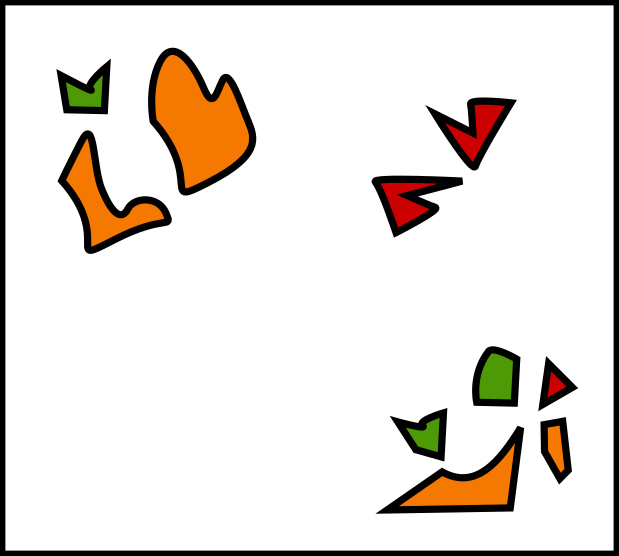
\includegraphics[width=\textwidth]{segmentation_lesions/GNN/etape1}
	\caption{Lésions originales issues du modèle de segmentation}
\end{subfigure}
\begin{subfigure}[t]{\colSize\textwidth}
	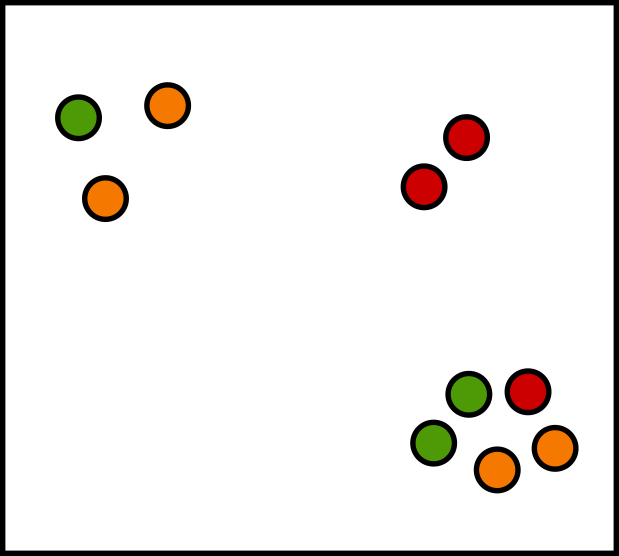
\includegraphics[width=\textwidth]{segmentation_lesions/GNN/etape2}
	\caption{Représentation sous forme d'un nuage de points.}

\end{subfigure}
\begin{subfigure}[t]{\colSize\textwidth}
	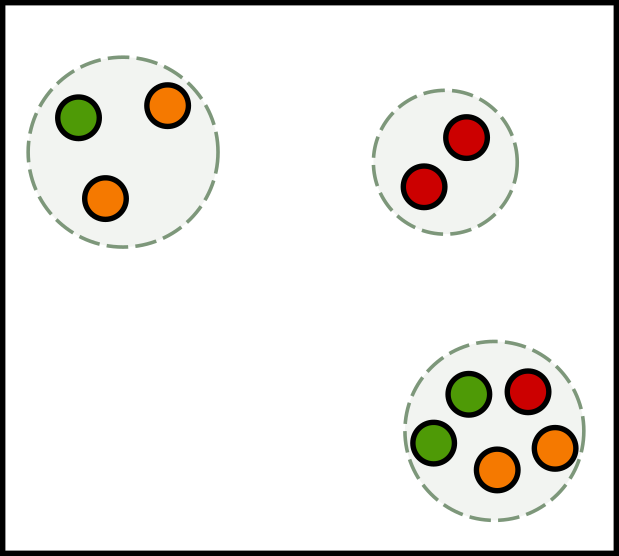
\includegraphics[width=\textwidth]{segmentation_lesions/GNN/etape3}
	\caption{Construction d'un graphe par plus proches voisins.}
	\label{subfig:StepAGraphConstruction}
\end{subfigure}
\begin{subfigure}[t]{\colSize\textwidth}
	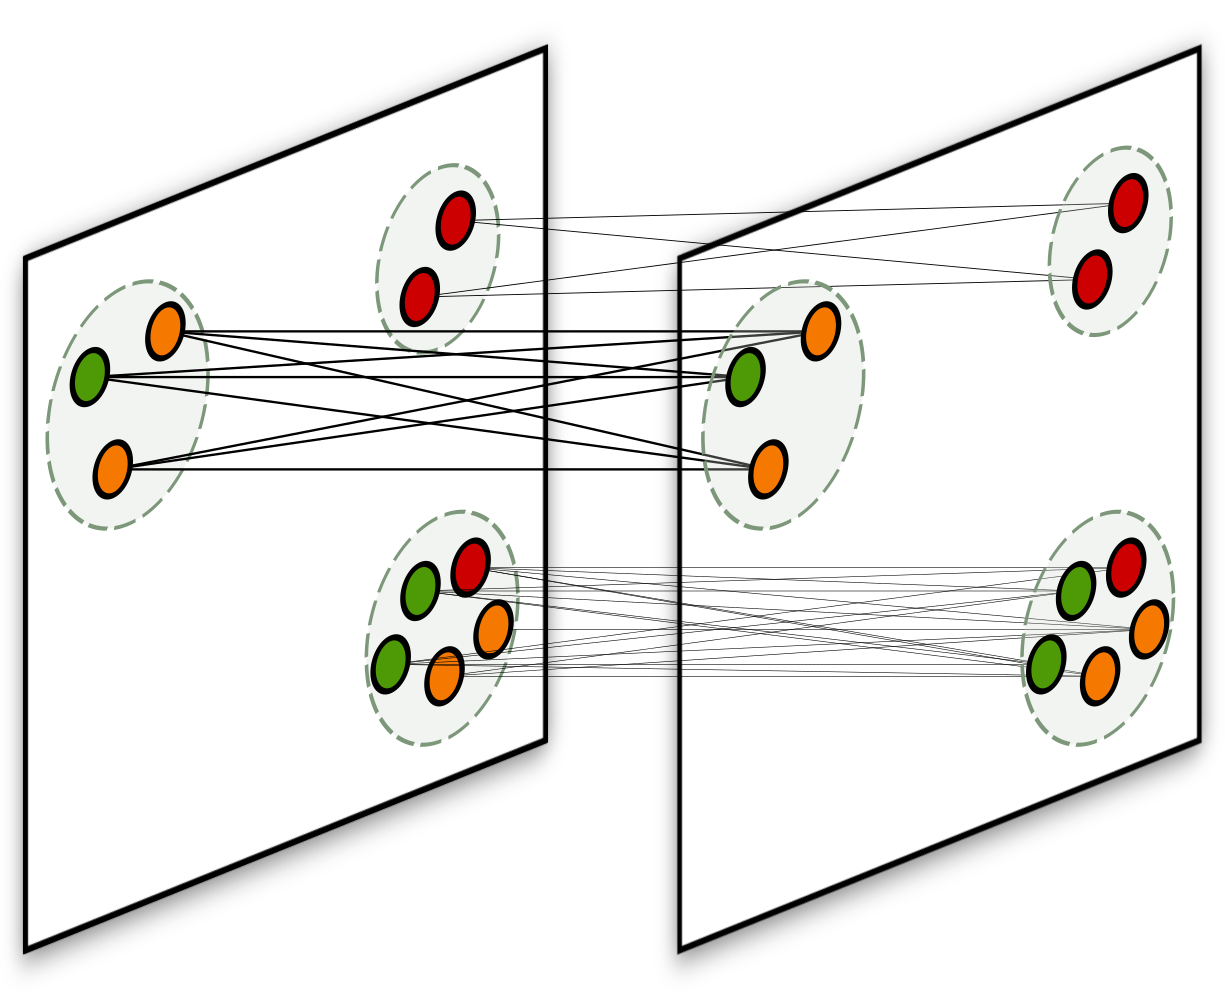
\includegraphics[width=\textwidth]{segmentation_lesions/GNN/etape4}
	\caption{Agrégation des caractéristiques entre \noeud s connectés.}
\end{subfigure}
\hfill
\begin{subfigure}[t]{\colSize\textwidth}
	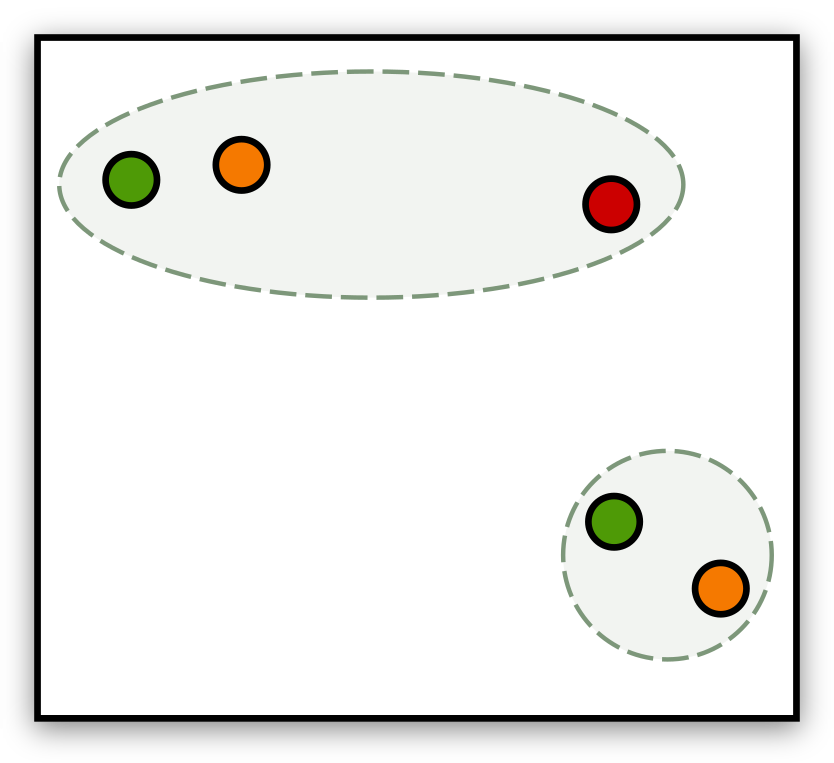
\includegraphics[width=\textwidth]{segmentation_lesions/GNN/etape5}
	\caption{Échantillonnage du graphe et reconstruction des relations d'adjacence.}
	\label{subfig:StepPointSampling}
\end{subfigure}
\begin{subfigure}[t]{\colSize\textwidth}
	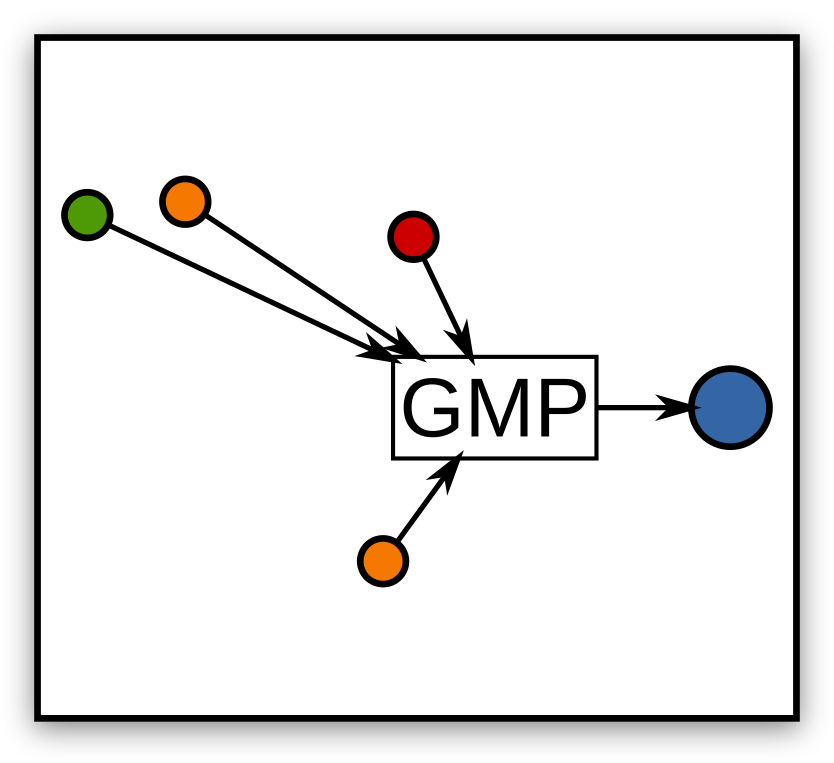
\includegraphics[width=\textwidth]{segmentation_lesions/GNN/etape_6}
	\caption{Fusion des \noeud s par \textit{Global Mean Pooling}.}
\end{subfigure}
\begin{subfigure}[t]{\colSize\textwidth}
	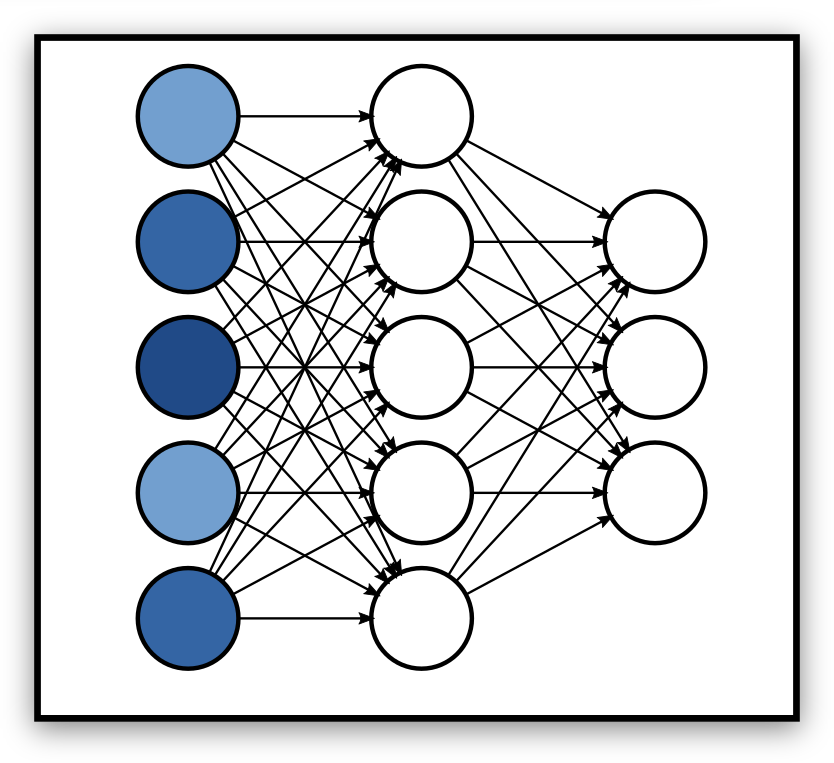
\includegraphics[width=\textwidth]{segmentation_lesions/GNN/etape_7}
	\caption{Classification du vecteur résultant.}
\end{subfigure}

\caption{Les différentes étapes mises en jeu dans l'architecture PointNet++, adaptée à la classification du graphe de lésions. Les étapes de \ref{subfig:StepAGraphConstruction} à \ref{subfig:StepPointSampling} représentent les opérations au c\oe ur d'une couche du réseau, répété $K$ fois (selon l'architecture)}
\label{fig:PointNetLesionsDRClass}
\end{figure}

Le PointNet++ attache donc une importance particulière à la position relative des lésions dans l'image, à la fois pour la construction initiale du graphe d'adjacence, le calcul de la transmission des messages (qui explicite la distance relative entre \noeud{}s dans les caractéristiques du message transmis) et le ré-échantillonnage entre blocs.

\subsubsection{Attention-GNN}
La seconde architecture que nous proposons est similaire à celle du PointNet++. Structurellement, elle repose sur le même principe de blocs au sein desquels sont transmis des messages de \noeud{}s en \noeud{}s. En revanche, nous remplaçons l'opérateur de transmission des messages du PointNet++ par le GATv2 (pour \textit{Graph Attention Network}) introduit par Brody et al. \cite{brody2022how}. Cet opérateur utilise un mécanisme d'attention similaire à celui des Transformers \cite{NIPS2017_3f5ee243} pour gérer la transmission de message entre \noeud{}s adjacents, à la seule différence que l'attention calculée est dynamique. 
Dans le détail, pour chaque \noeud{} $i$, l'équation de mise à jour son vecteur de représentation dans la couche $l$ est donnée par:
\begin{equation}
	h^{(l)}_i = \sigma(\sum_{j \in \mathcal{N}_i} \alpha_{ij}\cdot \mathbf{W}\mathbf{h_j})
\end{equation}
où $h^{(l)}_i \in \mathbb{R}^d$.
Le coefficient d'attention $\alpha_{ij}$ indique l'importance du \noeud{} $j$ vis-à-vis du \noeud{} $i$. Pour le calculer, on construit en premier lieu un score par arête unissant deux \noeud{}s adjacents.
\begin{equation}
	e(\mathbf{h}_i, \mathbf{h}_j) = \mathbf{a}^T \text{ReLU}(\mathbf{W}\cdot\left[\mathbf{h}_i || \mathbf{h}_j\right] )
\end{equation}
où $\mathbf{a} \in \mathbb{R}^{2d'}, \mathbf{W} \in \mathbb{R}^{2d'\times 2d}$ sont des paramètres appris du modèle et $||$ représente l'opérateur de concaténation. L'obtention d'$\alpha_{ij}$ se fait par une normalisation de type softmax de ce score d'arêtes:
\begin{equation}
	\alpha_{ij} = \frac{\exp(e(\mathbf{h}_i, \mathbf{h}_j))}{\sum_{j' \in \mathcal{N}_i} \exp(e(\mathbf{h}_i, \mathbf{h}_j'))}
\end{equation}

Cette architecture est donc plus complexe que le PointNet++, mais structurellement, elle respecte les mêmes principes.

\section{Protocole et résultats expérimentaux}


\subsection{Performances comparées entre les architectures de segmentation}
Afin de sélectionner un modèle parmi ceux présentés dans la section \ref{sec:segConceptionArchitecture}, un protocole expérimental standardisé a été mis en place. Celui-ci s'inspire du concours \ac{IDRiD} (dont est issue la base de même nom). Sur les 81 images de la base, 54 sont utilisées pour l'apprentissage (dont une fraction pour la validation), les 27 restantes pour l´évaluation du modèle. La métrique utilisée est l'\acl{AUC} -AUC- Précision/Sensibilité calculée sur 11 seuils uniformément répartis pour chaque lésion séparément. Pour nos entraînements, seules les données \ac{IDRiD} sont utilisées, en revanche, tous les encodeurs ont été pré-entraînés sur ImageNet. 
Les modèles sont entraînés avec un pas d'apprentissage de 0.001 et avec une dégradation de la pondération (\textit{weight decay}) de 0.00001 sur 1500 époques. Précisons qu'une époque correspond à un parcours de la base d'apprentissage. Comme les $\mathcal{B}^{(i)}$ varient en taille, les $\mathcal{M}[\mathcal{B}^{(i)}]$ ne sont donc pas tous entraînés avec le même nombre d'itérations totales ($= N_{\text{époques}} \times |\mathcal{B}^{(i)}|$). En revanche, chaque image est bien vue le même nombre de fois pour chaque entraînement. La fonction de coût utilisée est la généralisation différentiable du Dice introduite par Sudre et al. \cite{sudreGeneralisedDiceOverlap2017}. Différentes augmentations de données sont utilisées à la volée (modifications de contraste, luminosité, rotation, miroir...). Par ailleurs, lors de l'apprentissage, les images sont découpées en \og patchs \fg de taille $512 \times 512$.
 Les performances obtenues par les modèles sont rapportées dans le tableau \ref{tab:perfComparéeSegmentation}, qui offre une comparaison entre nos entraînements et les résultats rapportés dans la littérature. Toutes les combinaisons encodeur/décodeur mentionnées dans la section méthodologie (Tableau \ref{tab:segmentationNetworks}) n'apparaissent pas; cela s'explique du fait que notre processus de sélection s'appuie sur l'algorithme d'optimisation \textit{Hyperband} \cite{liHyperbandNovelBanditBased2018}, proposé par Li et al. Cet algorithme permet de mettre fin de manière prématurée aux entraînements (en l'occurence une des combinaison encodeur/décodeur) non-prometteurs. Pour cela, les performances sont suivies sur un ensemble de validation au cours de l'entraînement (on utilise le \textit{mIoU} comme métrique). Un budget est accordé à chaque entraînement (nombre d'itérations d'apprentissage à réaliser, temps maximum...) Ce budget est réactualisé en fonction des configurations d'entraînement les plus prometteuses. Celles qui ne le sont pas (c'est à dire qui n'intègre pas le top-k des meilleurs \textit{mIoU} obtenus jusqu'à présent) sont stoppées. Les autres voient leur budget augmenter et l'entraînement se poursuivre. Cette technique assure une économie significative de ressources lors d'une exploration de configurations. Le tableau \ref{tab:perfComparéeSegmentation} ne présente que les résultats des modèles ayant été entraînés en atteignant leur budget maximal.
\\
Les configurations potentielles ont été choisies pour couvrir un ensemble de modèles de tailles diverses, utilisant les techniques plurielles introduites dans notre état de l'art sur les architectures de réseau de neurones (section \ref{sec:segmentationFCCN}). Cet éventail couvre également des architectures mixtes, intégrant les récents modèles auto-attentifs de type \textit{Transformer} et \textit{Segformer}.

\begin{table}
	\centering
	\caption {Performances comparatives entre les différentes architectures testées. Les modèles sont entraînés et testés sur la base \ac{IDRiD} (séparée en deux ensembles suivant les règles de la compétition). En bleu sont indiqués nos scores les plus hauts, en gras, ceux de l'état de l'art.}
	\label{tab:perfComparéeSegmentation}
	\begin{threeparttable}
		\begin{tabular}{l lllll c}
			\toprule
			\multicolumn{7}{c}{Nos entraînements} \\
			\midrule
			Architecture & Encodeur & \ac{MA} & \ac{HEM} & \ac{CWS} & \ac{EX} & Moyenne\\
			\midrule
			\multirow{5}{3em}{UNet \cite{ronnebergerUNetConvolutionalNetworks2015a}}
			& ResNet - 18 \cite{zagoruykoWideResidualNetworks2016} & 0.4892 & 0.6407 & 0.7089 & 0.8512 & 0.6725 \\
			& ResNet - 34 & 0.4958 & 0.6457 & 0.7033 & 0.8415 & 0.6716 \\
			& ResNest - 50 \cite{zhangResNeStSplitAttentionNetworks2022} & 0.5041 & 0.6182 & 0.6289 & 0.821 & 0.6431 \\
			& SE ResNet - 50 \cite{huSqueezeandExcitationNetworks2018} & 0.4730 & 0.6111 & 0.6803 & 0.8233 & 0.6469 \\

			&  \tnote{1} MIT B2 \cite{xieSegFormerSimpleEfficient} & \color{blue}\textbf{0.5123} & 0.5749 & 0.7051 & 0.8408 & 0.6583 \\
			& \tnote{1} MIT B4 & 0.5045 & 0.6473 & 0.6959 & 0.8251 & 0.6682 \\
			\midrule
			\multirow{3}{3em}{UNet++ \cite{zhouUNetNestedUNet2018}} & ResNet - 18 & 0.4955 & 0.6348 & 0.7063 & \color{blue}\textbf{0.8531} & 0.6724 \\
			& ResNest - 50 & 0.4900 & 0.6601 & 0.6876 & 0.8019 & 0.6599 \\
			& SE ResNet - 50 & 0.4906 & 0.6141 & 0.7273 & 0.8169 & 0.6622 \\
			\midrule
			\multirow{4}{3em}{FPN \cite{seferbekovFeaturePyramidNetwork2018}} & ResNet - 18 & 0.4524 & 0.6476 & 0.7260 & 0.8229 & 0.6622 \\
			& ResNest - 50 & 0.4870 & \color{blue}\textbf{0.6898} & \color{blue}\textbf{0.7529} & 0.8246 & \color{blue}\textbf{0.6886} \\
			& SE ResNet - 50 & 0.4576 & 0.6790 & 0.7396 & 0.8169 & 0.6733 \\
			& MobileNet V3 \cite{sandlerMobileNetV2InvertedResiduals2018} & 0.3498 & 0.5828 & 0.6348 & 0.7509 & 0.5796 \\
			\midrule
			\multirow{3}{3em}{DeepLab V3+ \cite{chenDeepLabSemanticImage2018}} & ResNet - 18 & 0.4515 & 0.6426 & 0.6967 & 0.8098 & 0.6502 \\
			& ResNet - 34 & 0.4238 & 0.6073 & 0.6329 & 0.8329 & 0.6242 \\
			& SE ResNet - 50 & 0.4623 & 0.6868 & 0.7049 & 0.8204 & 0.6686 \\
			\midrule
			\tnote{3} Global-Local UNet & ResNest - 50 & 0.4580 & 0.6724 & 0.7080 & 0.8263 & 0.6662 \\
			\midrule
			\multicolumn{7}{c}{État de l'art publié}\\
			\midrule
			\multicolumn{2}{l}{L-Seg \cite{guoLSegEndtoendUnified2019}} & 0.4630 & 0.6370  & 0.7110 & 0.7950 & 0.6515 \\
			
			\multicolumn{2}{l}{Deep-Bayesian \cite{garifullinDeepBayesianBaseline2021}} & 0.4840 & 0.5930 & 0.6410 & 0.8420 & 0.6400 \\
			\multicolumn{2}{l}{\tnote{2} Global-Local UNet \cite{yanLearningMutuallyLocalGlobal2019}} & \textbf{0.5250} & \textbf{0.7030} & 0.6790 & \textbf{0.8890} & 0.6990 \\
			\multicolumn{2}{l}{CARNet \cite{guoCARNetCascadeAttentive2022}} & 0.5148 & 0.6389 & 0.7215 & 0.8675 & 0.6857 \\
			\multicolumn{2}{l}{\tnote{4} Xception-UNet - Collaborative learning \cite{zhouCollaborativeLearningSemiSupervised2019}} & 0.4960 & 0.6936 & \textbf{0.7407} & 0.8872 & \textbf{0.7044} \\
			\midrule
			\multicolumn{7}{c}{Classement officiel IDRiD \cite{porwalIDRiDDiabeticRetinopathy2020}}\\
			\midrule
			\multicolumn{2}{l}{Équipe} &  \\ 
			\midrule
			\multicolumn{2}{l}{VRT}& 0.4951 & 0.6804 & 0.6995 & 0.7127 & 0.6469 \\
			\multicolumn{2}{l}{PATech}& 0.4740 & 0.6490 & \multicolumn{1}{c}{-} & 0.8850 & \multicolumn{1}{c}{-}\\
			\multicolumn{2}{l}{iFLYTEK-MIG}& 0.5017 & 0.5588 & 0.6588 & 0.8741 & 0.6483 \\
			\multicolumn{2}{l}{SOONER}& 0.4003 & 0.5395 & 0.5369 & 0.7390 & 0.5539\\
			\bottomrule
		\end{tabular}
	\begin{tablenotes}
		\item[1] Encodeur de type \ac{VIT} suivant le modèle du SegFormer.
		\item[2] Il s'agit de quatre modèles distincts avec une architecture différente par lésion.
		\item[3] Notre réimplémentation est multi-classe (une seule architecture pour les quatre classes).
		\item[4] Ce modèle combine apprentissage supervisé et faiblement supervisé par entraînement adversarial, utilisant par conséquent beaucoup plus d'images.
	\end{tablenotes}
	\end{threeparttable}
\end{table}
\subsection{Étude empirique de la généralisation inter-bases}
\label{sec:generalisation_interbase}
La notion de généralisation est au cœur de la recherche sur la théorie de l'apprentissage statistique dont nous avons esquissé les contours dans la section \ref{sec:theorieApprentissage}. En revanche, nous abordons une approche résolument empirique, qui se détache des fondements théoriques. 
\subsubsection{Analyse quantitative des résultats}
Pour faciliter la lecture de notre analyse, nous introduisons les conventions de notation suivantes:
\begin{itemize}
	\item On introduit une indexation sur les différentes bases de données. Pour chaque base, les ensembles d'entraînement et d'évaluation sont référés en tant que  $\mathcal{B}^{(i)}$ et $\mathcal{B}^{(i)}_{\star}$ respectivement ($i  \in  \{I, M, D, R, F\}$, chaque base étant indexée par l'initiale de son nom). On note $\mathcal{S} = \bigcup_i^{\{I, M, D, R, F\}} \mathcal{B}^{(i)}$, c'est-à-dire l'union de toutes nos bases.
	\item Le modèle entraîné sur $\mathcal{B}^{(i)}$ est indiqué par $\mathcal{M}[\mathcal{B}^{(i)}]$. Ses prédictions sur la base $\mathcal{B}^{(j)}_{\star}$ sont notées $\mathcal{M}[\mathcal{B}^{(i)}](\mathcal{B}^{(j)}_{\star})$, ou $\mathcal{M}_{(i)}^{(j)^\star}$ en simplifié.
	\item Un modèle entraîné sur plusieurs bases de données est indiqué par $\mathcal{M}[\bigcup_i \mathcal{B}^{(i)}]$, ou, dans la version simplifiée, par $\mathcal{M}_\mathcal{S}$ quand l'entraînement se fait sur les cinq bases. 
	\item On note $D(\mathcal{M}_{(i)}^{(j)^\star}, \mathcal{B}^{(j)}_{\star})$ le score calculé sur les annotations de $\mathcal{B}^{(j)}_{\star}$ obtenu par le modèle entraîné sur la base $i$.
\end{itemize}

Afin de quantifier la notion de généralisation inter et intra-base, une même architecture est entraînée sur diverses bases de données $\mathcal{B}^{(i)}$ avant d'être évaluée sur $\mathcal{B}^{(j)}_{\star}$. Cette expérience permet de mettre en évidence la tendance du modèle à reproduire le style d'annotations propre à chaque base de données. En effet, comme cela se constate sur les résultats rapportés sur le tableau \ref{tab:generalisationPerfSegmentation}, quelle que soit la paire de bases d'apprentissage/test considérée, le meilleur score (en l'occurence le \ac{mIoU}) est toujours obtenu lorsque le jeu d'entraînement et le jeu d'évaluation sont issus de la même base. Autrement dit, formellement, nous observons la relation suivante:
\begin{equation}
	D(\mathcal{M}_{(i)}^{(i)^\star}, \mathcal{B}^{(i)}_{\star}) \geq D(\mathcal{M}_{(i)}^{(j)^\star}, \mathcal{B}^{(j)}_{\star}), \forall j
\end{equation}

À première vue, cela pourrait traduire une forme de sur-apprentissage sur une base de données (et donc d'une mauvaise généralisation). Mais cette interprétation est incomplète. En effet, au sens strict de la définition, nos modèles ne sur-apprennent pas: nous n'observons pas d'écart flagrant entre les métriques calculées sur $\mathcal{B}^{(i)}$ et $\mathcal{B}^{(i)}_{\star}$ (c'est-à-dire $D(\mathcal{M}_{(i)}^{(i)^\star},\mathcal{B}^{(i)}_{\star}) \approx D(\mathcal{M}_{(i)}^{(i)}, \mathcal{B}^{(i)})$). Par ailleurs, a minima sur IDRiD, les performances relevées sont de paire avec l'état-de-l'art, il n'existe donc pas de raisons de soupçonner un mauvais protocole d'entraînement. Comment expliquer la détérioration des métriques à travers les différents bases de test $\mathcal{B}^{(j)}_{\star}$ ? Notre hypothèse est que la notion de généralisation n'est a priori pas adaptée pour interpréter ces résultats, car elle repose sur le postulat de données indépendantes et identiquement distribuées selon une distribution $\mathbb{P}(X, Y)$ (images/annotations). À partir du moment où les données appartiennent à des distributions dissociées et bien distinctes, ce postulat ne tient plus et invalide la notion de généralisation. Or notre analyse préliminaire nous le confirme: bien que nous n'y ayons pas explicitement accès, la distribution statistique $\mathcal{B}^{(i)} \sim \mathbb{P}^{(i)}(X, Y)$ semble bien varier selon les bases. Plutôt que de parler de sur-apprentissage, nous introduisons par conséquent la notion de sur-sophistication d'un modèle sur une distribution. 
\\
Il existe a priori une manière simple de modéliser de manière plus représentative l'ensemble des données: entraîner le modèle à tirer parti de tous les différents styles d'annotations à la fois, c'est-à-dire lui faire apprendre la distribution $\bigcup_i \mathcal{B}^{(i)} \sim \mathbb{P}(X, Y)$. Ce modèle est noté $\mathcal{M}[\bigcup_i \mathcal{B}^{(i)}]$ et son entraînement consiste simplement à combiner toutes les bases. Dans nos travaux, cette combinaison est extrêmement simple, il s'agit d'une union des ensembles, sans ré-équilibrage. Il existe donc une forte disparité de représentativité de chaque base en terme de nombre d'échantillons; mais il n'est cependant pas évident qu'il soit nécessaire de corriger celle-ci. Notons qu'à la différence de la littérature sur la généralisation multi-domaines, nous ne définissons pas de domaine source ou cible. En effet, ces termes ont un sens lorsqu'on souhaite adapter un modèle d'un domaine vers l'autre (typiquement un généré artificiellement vers un réel). Pour notre application, nous n'avons aucune information a priori sur la pertinence clinique du style d'annotations donc pas d'incitations fortes à privilégier un domaine aux autres.
 \\
Nos résultats indiquent que l'efficacité de cette approche semble validée: sur trois des bases d'évaluation considérées $\mathcal{B}^{(j)}_{\star}$, ce modèle surpasse tous les autres:
\begin{equation}
	\label{eq:ParadoxalResults}
	 \exists k : D(\mathcal{M}_\mathcal{S}, \mathcal{B}^{(k)}_{\star}) > D(\mathcal{M}[\mathcal{B}^{(k)}], \mathcal{B}^{(k)}_{\star})
\end{equation}

Pour les deux autres cas de figure, la baisse des performances est relativement faible ($-0.0097$ pour MESSIDOR, $-0.0082$ pour \ac{DDR}). En revanche, la moyenne des scores est très nettement améliorée ($+0.125$) par rapport au second meilleur modèle.
\begin{table}
	\caption{Performance inter-bases: une même architecture est entraînée sur les différents sous-ensemble des données d'entraînements, dépendamment de leur base d'appartenance.}
	\label{tab:generalisationPerfSegmentation}
	\begin{tabularx}{\textwidth}{Xlllllc}
		\toprule
		\multirow{2}{3em}{Modèle} & \multicolumn{6}{c}{Score \ac{mIoU} sur les ensembles de test}\\
		\cmidrule{2-7}
		 & \ac{IDRiD}& MESSIDOR& \ac{DDR}& RET-LES& \ac{FGADR} & Moyenne\\
		\midrule
		$\mathcal{M}[\mathcal{B}^{(I)}]$ \ac{IDRiD} & \textbf{0.5546} & 0.3569 & 0.3192 & 0.2399 & 0.2535 & 0.3448 \\
		$\mathcal{M}[\mathcal{B}^{(M)}]$ MESSIDOR & 0.3807 & \textbf{0.4570} & 0.3079 & 0.2567 & 0.2157 & 0.3236 \\
		$\mathcal{M}[\mathcal{B}^{(D)}]$ \ac{DDR} & 0.5144 & 0.3410 & \textbf{0.4290} & 0.2529 & 0.2729 & 0.3620 \\
		$\mathcal{M}[\mathcal{B}^{(R)}]$ RET-LES & 0.2740 & 0.2804 & 0.2660 & \textbf{0.4940} & 0.2664 & 0.3162 \\
		$\mathcal{M}[\mathcal{B}^{(F)}]$ \ac{FGADR} & 0.3594 & 0.2616 & 0.2769 & 0.2392 & \textbf{0.4591} & 0.3192 \\
		\midrule
		$\mathcal{M}_\mathcal{S}$ & \textbf{0.6037} & 0.4473 & 0.4208 & \textbf{0.5025} & \textbf{0.4619} & \textbf{0.4872} \\
		\bottomrule
	\end{tabularx}
\end{table}
Une analyse plus fine est également proposée par lésions sur les graphiques de la figure \ref{fig:multilesionsGeneralisationScore}; mais elle ne révèle pas une tendance différente: en moyenne $\mathcal{M}_\mathcal{S}$ surpasse les autres modèles. Certes, un tel résultat est attendu sur le score moyen, ce modèle ayant été entraîné sur bien plus de données que tous les autres. Mais il est étonnant que l'amélioration ne soit pas qu'en moyenne, mais également sur les scores calculés séparément sur IDRiD, RET-LES et FGADR, ce que nous résumons formellement par l'équation \ref{eq:ParadoxalResults}. Cette équation relève d'un certain paradoxe: en effet, chaque ensemble $\mathcal{B}^{(j)}_{\star}$ ayant son propre style d'annotation, il semble impossible pour un modèle adoptant un certain style de maximiser les performances sur tous les autres, en particulier quand la différence de styles est aussi importante qu'entre RET-LES et IDRiD. Ce paradoxe nous pousse à explorer plus en détail le comportement du modèle $\mathcal{M}_\mathcal{S}$ dans la section qui suit.
\begin{figure}
	\centering
	\begin{subfigure}{.49\textwidth}
		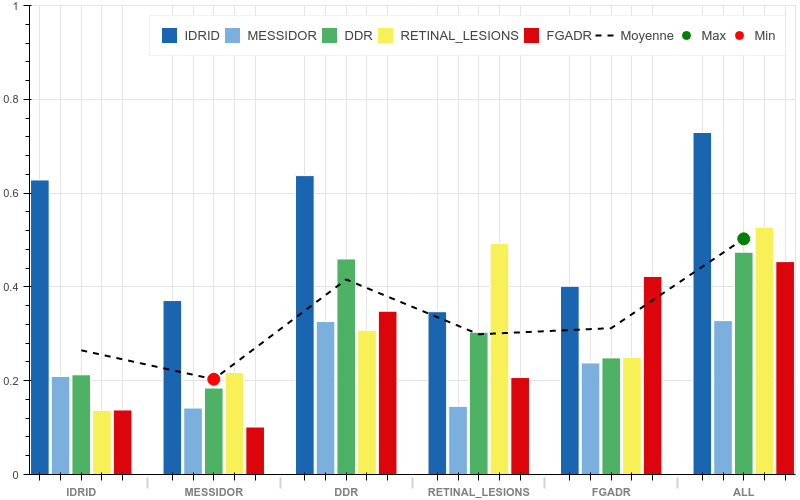
\includegraphics[width=.9\textwidth]{segmentation_lesions/generalisation/COTTON_WOOL_SPOT.png}
		\caption{Cotton Wool Spot}
	\end{subfigure}
	\begin{subfigure}{.49\textwidth}
		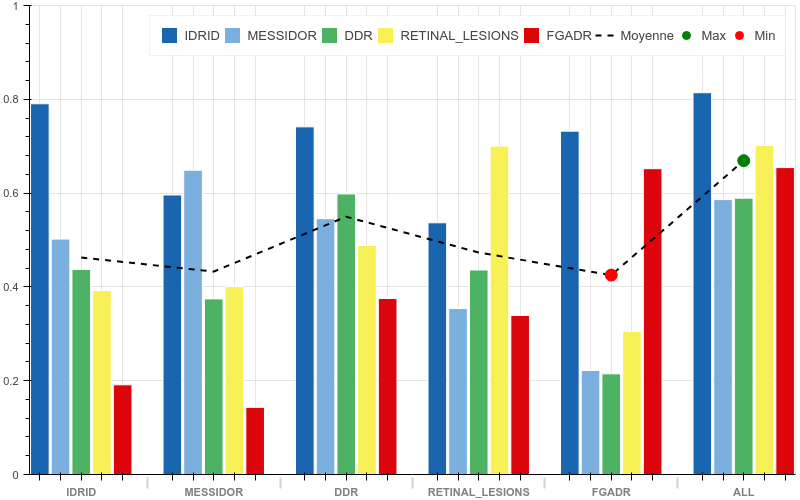
\includegraphics[width=.9\textwidth]{segmentation_lesions/generalisation/EXUDATES.png}
		\caption{Exsudats}
	\end{subfigure}
	\begin{subfigure}{.49\textwidth}
		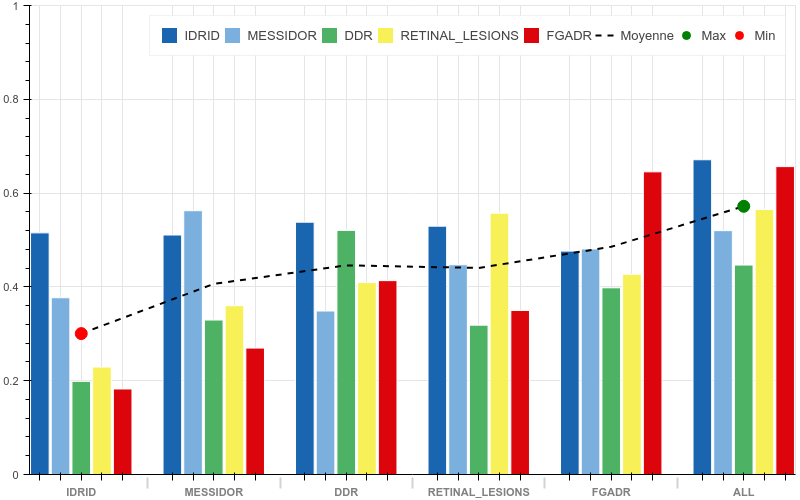
\includegraphics[width=.9\textwidth]{segmentation_lesions/generalisation/HEMORRHAGES.png}
		\caption{Hémorragies}
	\end{subfigure}
	\begin{subfigure}{.49\textwidth}
		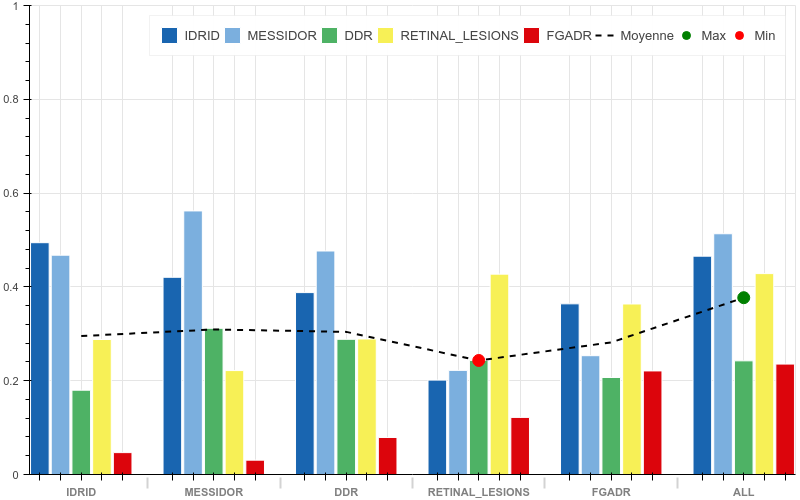
\includegraphics[width=.9\textwidth]{segmentation_lesions/generalisation/MICROANEURYSMS.png}
		\caption{Microanévrismes}
	\end{subfigure}
	\caption{Performance de généralisation par lésion. Suivant l'axe des abscisses sont indiquées les bases d'entraînements, en ordonnées, le score par base d'évaluation. Nous adoptons la métrique \ac{AUC} sous la courbe Précision/Sensibilité.}
	\label{fig:multilesionsGeneralisationScore}
\end{figure}
\subsubsection{Analyse qualitative}
\label{sec:SegmentationQualitativeAnalyse}
En complément de l'analyse quantitative, la figure \ref{fig:segQualitativeResults} propose un échantillon des prédictions réalisées par les différents modèles. Outre les quelques erreurs (sous ou sur-segmentation de certaines structures, confusions entre petites hémorragies et micro-anévrismes) visibles, il est particulièrement frappant d'observer à quel point le modèle entraîné sur une base imite le style d'annotations de celle-ci. Cet effet est particulièrement visible sur le modèle entraîné sur RET-LES. Ces observations qualitatives nous poussent à nous interroger sur la pertinence des métriques de segmentation utilisées, plus exactement sur la pertinence de les comparer entre elles à travers différentes bases et différents styles d'annotations. Pour explorer cette question, en annexe \ref{sec:AnnexeDetectionLesions}, nous proposons une analyse alternative reposant sur la capacité de détection des lésions et non plus sur leur segmentation.
\begin{figure}
	\centering
	\includegraphics[width=\textwidth]{segmentation_lesions/qualitative_results}
	\caption{Résultats qualitatifs de segmentation inter-bases. Chaque ligne représente un modèle entraîné sur une base. La dernière ligne correspond à la vérité terrain correspondante. Seules les frontières des structures segmentées sont représentées. \textbf{\textcolor{CWScolor}{\ac{CWS}}, \textcolor{EXcolor}{\ac{EX}}, \textcolor{HEcolor}{\ac{HEM}}, \textcolor{MAcolor}{\ac{MA}}}}
	\label{fig:segQualitativeResults}
\end{figure}

\renewcommand{\colSize}{0.26}
\begin{table}
	\caption{Illustration du phénomène du sur-sophistication d'un modèle sur un style d'annotations. Chaque ligne représente un ensemble de test, chaque colonne un modèle. $\mathcal{B}^{(I)}$ représente la base IDRiD, $\mathcal{B}^{(R)}$ la base RET-LES. La dernière colonne illustre le paradoxe du modèle combiné, capable d'adapter son style à la base de test.}
	\label{tab:IllustrationParadoxeModeleCombine}
	\begin{tabular}{m{2cm} ccc}
		\toprule
		& \multicolumn{3}{c}{Modèles} \\
		\midrule
		Bases de test & $\mathcal{M}[\mathcal{B}^{(I)}]$ & $\mathcal{M}[\mathcal{B}^{(R)}]$ &
		$\mathcal{M}[\bigcup_i \mathcal{B}^{(i)}]$ \\
		\midrule
		$\mathcal{B}^{(I)}_{\star}$ (IDRID)& 
		\begin{minipage}{\colSize\textwidth}
			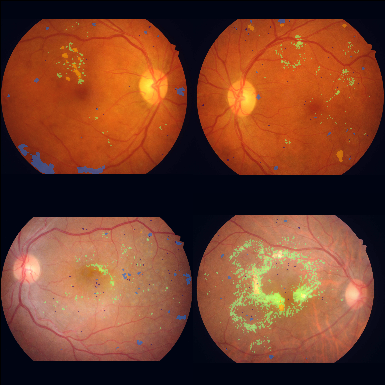
\includegraphics[width=\textwidth]{segmentation_lesions/generalisation/illustration/model_IDRID_images_IDRID.png} 
		\end{minipage} &
		\begin{minipage}{\colSize\textwidth} \includegraphics[width=\textwidth]{segmentation_lesions/generalisation/illustration/model_RETINAL_LESIONS_images_IDRID.png} 
		\end{minipage}& 
		\begin{minipage}{\colSize\textwidth}
			\includegraphics[width=\textwidth]{segmentation_lesions/generalisation/illustration/model_ALL_images_IDRID.png}
		\end{minipage} \\
		\midrule
		$\mathcal{B}^{(R)}_{\star}$ (RET-LES)&
		\begin{minipage}{\colSize\textwidth} \includegraphics[width=\textwidth]{segmentation_lesions/generalisation/illustration/model_IDRID_images_RETINAL_LESIONS.png}
		\end{minipage}&\begin{minipage}{\colSize\textwidth} \includegraphics[width=\textwidth]{segmentation_lesions/generalisation/illustration/model_RETINAL_LESIONS_images_RETINAL_LESIONS.png}
		\end{minipage}&\begin{minipage}{\colSize\textwidth} \includegraphics[width=\textwidth]{segmentation_lesions/generalisation/illustration/model_ALL_images_RETINAL_LESIONS.png}
		\end{minipage}\\
		\bottomrule
	\end{tabular}
\end{table}

\subsection{Adaptation de style par Attaque Adversariable}

\subsubsection{Paradoxe du modèle combiné $\mathcal{M}_{\mathcal{S}}$.}


Les résultats quantitatifs et qualitatifs obtenus des modèles $\mathcal{M}[\mathcal{B}^{(i)}]$ sont attendus: chaque modèle adopte le style d'annotations de sa base d'entraînement et obtient naturellement les meilleures performances sur l'ensemble de test correspondant. La surprise vient en revanche du modèle combiné:  $\mathcal{M}_{\mathcal{S}}$ parvient à surpasser simultanément trois de ces modèles sur leur propre base, ce qui représente un paradoxe apparent considérant que les styles d'annotations de chaque base ne sont pas mutuellement compatibles. On s'attendait alors à ce que le modèle adopte le style dominant (ou un style qui représente le meilleur compromis entre chaque base). L'observation des segmentations produites par $\mathcal{M}_{\mathcal{S}}$ résout ce paradoxe (voir le tableau \ref{tab:IllustrationParadoxeModeleCombine}) non sans soulever d'autres questions: on y voit que le modèle combiné est capable d'ajuster son style de segmentation en fonction de la base d'origine de l'image. Précisons bien qu'il s'agit d'images qui n'ont pas servi à l'entraînement du modèle, donc bien issues de l'ensemble d'évaluation. Le réseau n'a donc a priori pas d'informations sur le style d'annotations attendu, mais il arrive pourtant à identifier la base d'origine de l'image, et à adapter sa segmentation à un style concordant. Cette capacité lui permet donc d'obtenir des performances maximales sur les distributions distinctes de chaque base. Elle n'en reste pas moins surprenante: le modèle ne prend pour entrée qu'une image et n'a donc pas accès à son origine de manière explicite. L'unique explication est qu'il existe au sein d'une image un marqueur permettant d'identifier sa base d'appartenance. Le modèle $\mathcal{M}_{\mathcal{S}}$ apprend à reconnaître ce marqueur, à le lire à l'inférence et modifier sa sortie en fonction. Et bien qu'innattendu, cet effet peut s'expliquer: les différentes bases contiennent en leur sein des images dont l'intra-variabilité est plus faible que l'inter-variabilité entre bases. En effet,  au sein d'une même base, les images sont acquises dans des conditions relativement homogènes: c'est-à-dire même matériel d'acquisition et résolution d'acquisition. Par ailleurs, on peut aussi supposer d'une ethnicité relativement homogène au sein de la population représentée dans chaque base. L'hypothèse d'un marqueur de base identifiable dans chaque image n'est donc pas invraisemblable. 
\\
Mais une fois ce comportement de $\mathcal{M}_\mathcal{S}$ identifié, plusieurs questions se posent:
\begin{itemize}
	\item Est-il possible d'identifier le marqueur implicite contenu dans l'image qui trahit son origine?
	\item Comment le modèle de segmentation lit-il ce marqueur pour ajuster sa prédiction?
	\item Finalement, peut-on contraindre de manière prédictible le style de segmentation du modèle en manipulant ce marqueur de base?
\end{itemize}

Précisons que par la suite, nous prendrons souvent IDRiD et RET-LES en exemple car ces deux bases sont les plus radicalement différentes dans leur style d'annotations respectif.
\subsubsection{Robustesse de l'identification de base}
De manière préliminaire, nous avons voulu tester la sensibilité de la phase d'identification du marqueur lorsqu'on soumet l'image fournie au modèle à diverses perturbations simples. Pour nos expériences, celles-ci sont de deux types: géométriques ou colorimétriques. Dans le premier cas, on sous-échantillonne l'image (par un facteur 4) avant de la redimensionner à son échelle originale. Cette opération est équivalente à l'application d'un filtre passe-bas et simule une résolution d'acquisition variable. Elle vise à vérifier que le marqueur d'appartenance à une base n'est pas liée à une certaine composante haute fréquence imperceptible présente dans l'image. La seconde opération modifie de manière aléatoire la teinte, la saturation, la luminosité et le contraste de l'image (dans la limite de 20\% d'altérations). Enfin, pour évaluer si la distinction entre base ne provient pas de la compression choisie des images, nous étudions l'effet de celle-ci dans un scénario exacerbé (réduction par compression JPEG à 40\% du poids en octet de l'image originale). Comme en témoignent les résultats sur le tableau \ref{tab:PerturbationsIdentificationsMarqueursDB}, aucune de ces approches ne perturbe le style de segmentation choisi par le réseau de manière probante, à l'exception dans une moindre mesure de la compression JPEG.

\renewcommand{\colSize}{0.3}
\begin{table}
	\centering
	\caption{Pour identifier le marqueur de base de données dans l'image, des perturbations géométriques ou colorimétriques sont appliquées à celle-ci. Ces perturbations n'ont pas d'effet sur le style de segmentation choisi par le modèle. Marginalement, le niveau de compression peut avoir un léger effet sur $\mathcal{B}^{(I)}_{\star}$.}
	\label{tab:PerturbationsIdentificationsMarqueursDB}
	\begin{tabular}{m{5cm} cc}
		\toprule
		Modèles & \multicolumn{2}{|c}{Bases} \\
		\midrule
		 & $\mathcal{B}^{(I)}_{\star}$ (IDRID)& $\mathcal{B}^{(R)}_{\star}$ (RET-LES)\\
		\midrule
		$\mathcal{M}[\bigcup_i \mathcal{B}^{(i)}]$ (Référence) & 
		\begin{minipage}{\colSize\textwidth}
		\includegraphics[width=\textwidth]{segmentation_lesions/generalisation/CombinedModelTricking/model_ALL_images_IDRID_ref}
		\end{minipage}
	& 
	\begin{minipage}{\colSize\textwidth}
		\includegraphics[width=\textwidth]{segmentation_lesions/generalisation/CombinedModelTricking/model_ALL_images_RETINAL_LESIONS_ref}
	\end{minipage}
	\\
	\midrule
	\midrule
	$\mathcal{M}[\bigcup_i \mathcal{B}^{(i)}]$ + 
	Variation d'échelle (résolution $\times 25\%$) & \begin{minipage}{\colSize\textwidth}
		\includegraphics[width=\textwidth]{segmentation_lesions/generalisation/CombinedModelTricking/model_ALL_images_IDRID_randomResize}
	\end{minipage}
	& 
	\begin{minipage}{\colSize\textwidth}
		\includegraphics[width=\textwidth]{segmentation_lesions/generalisation/CombinedModelTricking/model_ALL_images_RETINAL_LESIONS_randomResize}
	\end{minipage} \\
\midrule
$\mathcal{M}[\bigcup_i \mathcal{B}^{(i)}]$ +
		Variation colorimétrique (saturation, teinte, contraste, luminosité) & \begin{minipage}{\colSize\textwidth}
			\includegraphics[width=\textwidth]{segmentation_lesions/generalisation/CombinedModelTricking/model_ALL_images_IDRID_colorJitter}
		\end{minipage}
		& 
		\begin{minipage}{\colSize\textwidth}
			\includegraphics[width=\textwidth]{segmentation_lesions/generalisation/CombinedModelTricking/model_ALL_images_RETINAL_LESIONS_colorJitter}
		\end{minipage} \\
	\midrule
	$\mathcal{M}[\bigcup_i \mathcal{B}^{(i)}]$ + 
	Compression JPEG (40\%) 
	& \begin{minipage}{\colSize\textwidth}
		\includegraphics[width=\textwidth]{segmentation_lesions/generalisation/CombinedModelTricking/model_ALL_images_IDRID_compression}
	\end{minipage}
	& 
	\begin{minipage}{\colSize\textwidth}
		\includegraphics[width=\textwidth]{segmentation_lesions/generalisation/CombinedModelTricking/model_ALL_images_RETINAL_LESIONS_compression}
	\end{minipage} \\
		\bottomrule
	\end{tabular}
\end{table}


\subsubsection{Classification de l'origine de l'image}
L'approche par perturbations simples ne permettant pas d'expliquer le comportement du modèle, nous adoptons une méthode inspirée par les travaux de Alain et al. \cite{DBLP:conf/iclr/AlainB17}. Pour comprendre les caractéristiques lues par un modèle, ces derniers proposent d'inspecter les différentes couches d'un réseau en utilisant des sondes linéaires prenant pour entrée les cartes caractéristiques issues de chaque couche et tentant de les classifier. La linéarité de ces sondes n'est pas en soi indispensable mais elle confère un caractère interprétable. Par ailleurs, il est pertinent de garder un modèle simple de sonde car ce n'est pas son pouvoir discriminant qui présente un intérêt, mais celui des caractéristiques issues du réseau inspecté. \\
De façon équivalente, nous proposons d'entraîner un micro-modèle pour sonder les caractéristiques extraites de l'encodeur du modèle de segmentation. Ce dernier est gelé, autrement dit ses poids ne seront pas modifiés. Le positionnement de la sonde (c'est-à-dire la profondeur de la couche sondée dans l'encodeur) est un paramètre expérimental. La sonde a pour objectif de prédire l'origine de l'image d'entrée, c'est-à-dire sa base d'appartenance parmi les cinq que nous utilisons. Le modèle de sonde employé n'est pas linéaire pour des raisons pratiques de convergence mais il repose sur une architecture extrêmement simple. Nous l'illustrons sur la figure \ref{fig:ModeleSondeClassifDatabase}.
La sonde, dénotée $s$, est entraînée à minimiser la fonction d'entrophie croisée:
\begin{equation}
	\mathcal{L}(x_n, y_n) = \sum_{c=1}^{C} \log s(x_{n})_c \cdot y_{n, c}
\end{equation}
où $x_n$ est l'image d'entrée, $s(x_{n, c})$ la probabilité d'appartanence à la base de données $c$ prédite par le modèle et $y_{n, c}$ la vérité terrain.
\begin{figure}[h!]
	\centering
	\includegraphics[width=.8\textwidth]{segmentation_lesions/sonde_database}
	\caption{Modèle de sonde utilisé pour la classification de l'origine des données. Les flèches pointillées indiquent les différents points de connexion, mais il s'agit bien de quatre sondes distinctes, bien que basées sur la même architecture.}
	\label{fig:ModeleSondeClassifDatabase}
\end{figure}
 
En pratique, nous avons entraîné séparément différentes sondes, une par couche d'encodeur. Chacune d'entre elles est entraînée sur trois époques sur l'ensemble des données $\bigcup_i \mathcal{B}^{(i)}$. Les résultats sont fournis sur le graphique de la figure \ref{fig:classifDataset}. Pour en faciliter l'interprétation, nous avons équilibré les cinq classes (correspondant chacune à une base de données). Avec près de 97\% des images correctement classifiées dans le meilleur cas, force est de constater que la classification de l'origine des données ne pose pas problème à la sonde. La performance tend à s'améliorer fortement vers les couches les plus profondes du réseau de segmentation. Cela confirme la capacité du modèle à progressivement décoder ce marqueur dans l'image d'entrée. Dans le détail, notons que sur le graphique de la figure \ref{fig:classifDataset}, l'indice 0 correspond à l'image brute. Rien qu'à partir de celle-ci, la sonde prédit la base d'appartenance d'origine avec une exactitude de près de 60\%. Ce chiffre grimpe jusqu'à 97\% pour la sonde placée sur l'avant-dernière couche de l'encodeur. Pour celle-ci, nous étoffons notre analyse en calculant la matrice de confusion des prédictions réalisées, rapportée sur la figure \ref{fig:confMatProbeRef}. Dans le détail par classe, on observe que la plus grande source d'erreur provient d'images de MESSIDOR et IDRID (respectivement 28.4\% et 17.2\% de ces deux bases) prédites comme appartenant à DDR par la sonde. Cela témoigne a priori d'une grande proximité entre ces trois bases, en accord avec notre analyse préliminaire de la section \ref{sec:variabilitéSegmentation}.
Quoiqu'il en soit, l'existance d'un identifiant indiquant la base d'origine inscrit dans l'image et décodé progressivement par le modèle de segmentation se confirme à travers nos résultats.

\begin{figure}
	\centering
	\includegraphics[width=.7\textwidth]{segmentation_lesions/generalisation/accuracy_dataset_classif}
	\caption{Performance de classification de l'origine des images ($\mathcal{B}^{(i)}$) suivant la couche d'encodage sondée dans le modèle de segmentation.}
	\label{fig:classifDataset}
\end{figure}

\begin{figure}
	\centering
	\includegraphics[width=.7\textwidth]{segmentation_lesions/probing/probe_confMat}
	\caption{Matrice de confusion obtenue à partir des prédictions de la sonde située dans l'avant dernière couche d'encodage du modèle de segmentation.}
	\label{fig:confMatProbeRef}
\end{figure}


\paragraph{Adaptation par conversion adversariale}
La facilité de classification de l'origine de l'image par la sonde interroge sur les caractéristiques lues dans celle-ci permettant cette classification. Répondre à cette question offre indirectement une opportunité de premier choix: est-il possible de modifier l'image d'entrée de telle sorte à tromper la sonde? Si tel est le cas, l'effet se répercute-t-il sur le modèle de segmentation (décodeur inclus)? Enfin, ce faisant, peut-on le contraindre à adopter un style d'annotations choisi? \\

Pour étudier ces questions, nous avons mis au point une expérience basée sur le principe des attaques adversariales. Cette technique vise à modifier imperceptiblement l'entrée d'un réseau de telle sorte à le tromper dans sa classification et à détourner sa prédiction originale vers une classe cible choisie. Dans notre cas, l'attaque est portée sur la sonde de classification dans le but de lui faire prédire une base de données $T$ choisie sur n'importe quelle image qui lui est proposée. Les travaux existants sur les attaques adversariales suggèrent diverses modifications de l'image pour atteindre cet objectif. La plus courante est de rétro-propager les gradients de la fonction de coût évaluée sur la cible $T$ jusqu'à l'entrée. On modifie ensuite celle-ci par descente de gradients dans la direction qui minimise ce coût (et maximise donc la prédiction $T$). Il existe une abondante littérature sur le sujet, en général orientée vers la question de la cyber-sécurité des réseaux de neurones, car le principe des attaques adversariales repose sur l'exploitation d'une de leur vulnérabilité intrinsèque (la sensibilité au gradient). Notre application est transverse à ces questions, car notre objectif est de caractériser la capacité d'adaptation à divers domaines de distribution. Par ailleurs, nous souhaitons bien mettre l'accent sur le fait que l'attaque adversariale a ici pour but de tromper la sonde et non le modèle de segmentation. L'effet sur ce dernier, bien que nous verrons qu'il est radical, en est une conséquence indirecte.

Nous utilisons l'approche de Madry et al. \cite{DBLP:conf/iclr/MadryMSTV18} pour concevoir notre attaque:
soient $x$ l'image initiale (issue de $\mathcal{B}_{\star}$) et $t$ la classe que l'on souhaite faire prédire à la sonde. La création d'une image adversariale s'obtient suivant la procédure itérative suivante:
\begin{align}
	x_0 &= x \nonumber \\
	x_{k+1} &= \mathcal{S}_\epsilon(x_k - \alpha \cdot \text{signe}(\nabla \mathcal{L}(x_k, t))), k \in \left\lbrace 1,...,K
	\right\rbrace 
	\label{eq:adversarialExample}
\end{align}
où $\mathcal{S}_\epsilon$ est une fonction qui restreint la perturbation dans une boule centrée sur $x$ de rayon $\epsilon$. On reconnaîtra ici une équation très similaire à celle de la descente de gradients; précisons simplement qu'ici, seule l'image d'entrée est modifiée et non les poids ni de la sonde, ni du réseau de segmentation. L'équation \ref{eq:adversarialExample} se répète $K$ fois et l'image résultante $x_K$ est théoriquement censée perturber la prédiction de la sonde vers la classe choisie. Par ailleurs, en contraignant un $\epsilon$ petit, on force cette modification à rester imperceptible à l'\oeil{} humain. \\
Pour nos expériences, nous utilisons $\epsilon=0.025$, un pas de modification $\alpha = 0.002$ et $K=15$ étapes. Du fait du petit $\epsilon$, les perturbations sont a priori imperceptibles à l'\oeil{} humain: les valeurs de pixels de l'image étant comprises dans l'intervalle $\left[-1, 1\right]$, elles ne peuvent être modifiées au maximum que de $0.125\%$. \\
Pour simplifier la lecture des résultats, nous introduisons une nouvelle notation: $\mathcal{B}^{(i)} \Rightarrow \mathcal{B}^{(j)}$ indique une conversion adversariale des images de la base source $\mathcal{B}^{(i)}$ vers la base cible $\mathcal{B}^{(j)}$. Ainsi $M( \mathcal{B}_\star^{(j)} \Rightarrow \mathcal{B}^{(i)})$ signifie que le modèle $M$ est testé sur des images appartenant à $\mathcal{B}_\star^{(j)}$ qui ont été modifiées pour correspondre à la base  $\mathcal{B}^{(i)}$. Nous pouvons quantifier le succès de conversion, en observant la proportion d'images classées $T$ par la sonde après conversion $\bigcup_i \mathcal{B}^{(i)}_\star \Rightarrow \mathcal{B}^{(T)}$. Les résultats sont rapportés sur la figure \ref{fig:labelConversionSuccess}. Dépendamment de la cible $T$, le taux de conversion réussie varie entre  82.5\% (vers IDRID) et 65.2\% (vers MESSIDOR). Dans le détail, les images issues FGADR sont celles les plus difficilement converties, avec 15.3\% de conversion ratées provenant d'images de cette base (pour la conversion vers IDRID), 21.4\% (vers MESSIDOR) et 33.5\% (vers RETINAL-LESIONS). Si on exclue FGADR de nos images de test, le taux de succès de conversion moyen (toute base confondue) est de 90.5\%, le taux le plus faible étant pour la conversion vers FGADR (79\% de succès) et le plus élevé pour RETINAL-LESIONS (98.8\%).

\begin{figure}
	\centering
	\includegraphics[width=\textwidth]{segmentation_lesions/probing/accuracy_probe_after_convert}
	\caption{Pourcentage d'images des bases $\bigcup_i \mathcal{B}^{(i)}$ classées $T$ par la sonde après conversion $\bigcup_i \mathcal{B}^{(i)} \Rightarrow \mathcal{B}^{(T)}$. Cette proportion correspond au taux d'images ayant trompé la sonde après conversion vers la cible $T$ visée.}
	\label{fig:labelConversionSuccess}
\end{figure}

Cependant, tromper la sonde n'est pas notre objectif en soi. Dans le contexte de notre étude d'inter-généralisation, il est plus intéressant d'observer comment l'image transformée impacte la prédiction du modèle de segmentation. Dans le tableau \ref{tab:AdversarialAttackResult}, nous illustrons l'effet de la conversion sur le modèle. La sonde choisie est connectée à l'avant-dernière couche de l'encodeur et nous avons expérimenté avec deux types de conversions (vers IDRID et vers RETINAL-LESIONS). Considérant que toutes les segmentations du tableau sont réalisées avec le même modèle inchangé et sur des images de test, les résultats obtenus se révèlent déroutants: les modifications adversariales apportées à l'image d'entrée permettent de drastiquement modifier le style de segmentation. Ce faisant, nous obtenons une très grande flexibilité sur le style de segmentation en sortie: un même modèle peut-être configuré, sans avoir à le modifier et donc sans ré-entraînement coûteux, à adopter un style de segmentation parmi plusieurs alternatives. Qui plus est, le processus de conversion est stable: la conversion $\mathcal{B}^{(i)} \Rightarrow \mathcal{B}^{(i)}$ ne modifie pas la segmentation du modèle.

\renewcommand{\colSize}{0.40}
\begin{table}
	\caption{L'attaque adversariale de la sonde de classification modifie de manière imperceptible à l'\oeil{} nu l'image d'entrée. En revanche, elle permet de drastiquement modifier la segmentation pour adopter un style au gré de l'utilisateur.}
	\label{tab:AdversarialAttackResult}
	\begin{tabular}{m{2cm} cc}
		\toprule
		Modèles & \multicolumn{2}{|c}{Bases} \\
		\midrule
		& $\mathcal{B}^{(I)}_{\star}$ & $\mathcal{B}^{(R)}_{\star}$ \\
		
		$\mathcal{M}[\bigcup_i \mathcal{B}^{(i)}]$ (Référence) & 
		\begin{minipage}{\colSize\textwidth}
			\includegraphics[width=\textwidth]{segmentation_lesions/generalisation/CombinedModelTricking/model_ALL_images_IDRID_ref}
		\end{minipage}
		& 
		\begin{minipage}{\colSize\textwidth}
			\includegraphics[width=\textwidth]{segmentation_lesions/generalisation/CombinedModelTricking/model_ALL_images_RETINAL_LESIONS_ref}
		\end{minipage}
		\\
		\midrule
		\midrule
		$\mathcal{M} \Rightarrow \mathcal{B}^{(I)} $ &
		\begin{minipage}{\colSize\textwidth}
			\includegraphics[width=\textwidth]{segmentation_lesions/generalisation/CombinedModelTricking/model_ALL_images_IDRID_adversarial_ref}
		\end{minipage}
		&
		\begin{minipage}{\colSize\textwidth}
			\includegraphics[width=\textwidth]{segmentation_lesions/generalisation/CombinedModelTricking/model_ALL_images_RETINAL_LESIONS_adversarial}
		\end{minipage} 
		\\
		\midrule
		$\mathcal{M} \Rightarrow \mathcal{B}^{(R)} $ &
		\begin{minipage}{\colSize\textwidth}
			\includegraphics[width=\textwidth]{segmentation_lesions/generalisation/CombinedModelTricking/model_ALL_images_IDRID_adversarial}
		\end{minipage}
		&
		\begin{minipage}{\colSize\textwidth}
			\includegraphics[width=\textwidth]{segmentation_lesions/generalisation/CombinedModelTricking/model_ALL_images_RETINAL_LESIONS_adversarial_ref}
		\end{minipage}
		\\
		\bottomrule
	\end{tabular}
\end{table}
 
\paragraph{Validation quantitative}

L'efficacité du processus de conversion des images reste encore à démontrer. À défaut d'avoir plusieurs styles d'annotations pour une même image, nous disposons de modèles dont nous savons qu'ils ont chacun adopté un style d'annotations spécifique (les $\mathcal{M}[\mathcal{B}^{(i)}]$). Ceux-ci nous serviront pour notre protocole d'évaluation. Notre objectif est d'éprouver la fiabilité du processus de conversion adversariale dans un contexte pseudo-clinique, donc sur des images qui n'appartiennent à aucune des bases utilisées jusqu'à présent. Nous prélevons pour cela un sous-ensemble de 100 images issues de la base APTOS, pour lesquelles nous ne disposons pas d'annotations de lésions. On note $\mathcal{K}$ cet ensemble. À partir de chacun des modèles $\mathcal{M}[\mathcal{B}^{(i)}]$, on génère cinq styles d'annotations de segmentations qui nous serviront de référence. Elles seront comparées avec les segmentations de $\mathcal{M}[\bigcup_i \mathcal{B}^{(i)}]$ après conversion adversariale vers chacune des bases. Formellement, notre validation repose donc sur l'évaluation de la métrique $D$ entre les modèles spécialisés et le modèle de référence après conversion des images vers le domaine de chaque modèle spécialisé:
\begin{equation}
	D(\mathcal{M}_{(j)}(\mathcal{K}), \mathcal{M}_\mathcal{S}(\mathcal{K} \Rightarrow \mathcal{B}^{(t)})), \forall j, t
\end{equation}
À l'instar de nos précédentes expériences, nous utilisons la mIoU comme métrique de comparaison. Les résultats sont synthétisés sur la matrice représentée sur la figure \ref{fig:ValidationConversionTable}. L'intérêt de ces résultats apparaît par une lecture ligne à ligne de la matrice fournie. En particulier, on observe que;
\begin{equation}
	D(\mathcal{M}_{(j)}(\mathcal{K}), \mathcal{M}_\mathcal{S}(\mathcal{K} \Rightarrow \mathcal{B}^{(j)})) \geq D(\mathcal{M}_{(j)}(\mathcal{K}), \mathcal{M}_\mathcal{S}(\mathcal{K} \Rightarrow \mathcal{B}^{(t)})), \forall j, t
\end{equation}
Autrement dit, après conversion vers la classe $T$, le modèle $\mathcal{M}_\mathcal{S} \Rightarrow T$ s'approche systématiquement le plus du modèle $\mathcal{M}_T$. Ce résultat confirme l'efficacité de l'approche adversariale pour modifier au choix le style de segmentation au modèle. 
\begin{figure}
	\centering
	\includegraphics[width=.6\textwidth]{segmentation_lesions/generalisation/validation_conversion}
	\caption{Cette matrice représente le score mIoU obtenu en comparant les prédictions réalisées par chacun des modèles spécialisés $\mathcal{M}_{(j)}$ et celles réalisées par le modèle $\mathcal{M}_\mathcal{S}$ après conversion adversariale des images d'entrées vers chacune des bases.}
	\label{fig:ValidationConversionTable}
\end{figure}


\subsection{Classification de la rétinopathie diabétique par \ac{GNN}}
Afin de pousser l'exploration sur la qualité des lésions, nous proposons de reconstituer le diagnostic de l'image à partir des cartes de segmentation produites par les différents modèles $\mathcal{M}[\mathcal{B}^{(i)}]$. Deux architectures de classification sont comparées, telles que décrites dans la section méthodologique. L'entraînement est réalisé sur les 35126 images de l'ensemble d'apprentissage de la base EyePACS. $5\%$ de ces images sont utilisées pour la validation du modèle. Le modèle qui obtient le meilleur score de validation au cours de 250 époques est ensuite évalué sur les bases Aptos et EyePacs (test). 
Les résultats sont  reportés dans le tableau \ref{tab:PerfGNNClassification}. En moyenne, quelque soit le modèle de segmentation (hormis celui entraîné sur IDRiD), l'architecture Att-GNN obtient les meilleures performances. Notamment, ce constat est particulièrement notable sur l'ensemble de test EyePacs, composé d'images de bien moins bonne qualité que sur Aptos.
\\
Dans le détail, on observe également la supériorité (en moyenne sur les deux ensembles) des performances obtenues avec $\mathcal{M}_\mathcal{S}$ obtenant respectivement 0.735 (Att-GNN) et 0.682 (PointNet++), suivi de $\mathcal{M}[\mathcal{B}^{(R)}]$ (scores respectivement de 0.714 et 0.663). \\
Relativement à ce que produit un CNN à partir d'une image, ces scores ne sont pas élevés, notamment par rapport à ceux obtenus dans l'étude préliminaire de la section \ref{sec:preliminaryExperimentClassSegm}. En les analysant plus finement, il apparaît que les modèles par graphe peinent surtout à distinguer certaines classes, en particulier la rétinopathie proliférative. Ce phénomène n'est pas surprenant, dans la mesure où ce grade de la maladie se détecte par l'apparition de néo-vaisseaux; or, nos modèles de segmentation ne sont pas entraînés à détecter ceux-ci. Pour mieux quantifier le potentiel de l'approche par graphe, nous simplifions donc le problème posé, en regroupant les classes 0 et 1 d'une part (non malade et bénigne) et les classes 2,3,4 d'autre part (modérée, sévère et proliférative.) Ce choix correspond aux recommandations dans le cadre de campagne de dépistage de la \ac{RD}. On obtient alors les performances reportées dans le tableau \ref{tab:DetectionRDScoreGraph}. Dans le meilleur des cas, nous obtenons un couple Sensibilité/Spécificité de détection de 96.57\%/81.29\% sur Aptos et de 52.77\%/98.06\% sur EyePacs. On peut s'étonner d'une telle différence de sensibilité entre les deux bases: elle s'explique notamment par le fait que la base EyePACS contient notoirement énormément d'images de mauvaises qualités. Sur celles-ci, le réseau de segmentation tend à sous-segmenter les lésions en raison de la faible lisibilité de l'image. Inversement, Aptos est plus homogène, on obtient donc de meilleurs résultats de segmentation dessus. Ce dernier point confirme donc la nécessité d'utiliser des images de bonne qualité dès lors qu'on utilise la segmentation pour classifier les images de \fundus{}.

\begin{table}
	\caption{Performances de classification (gradation en 5 classes) de la rétinopathie diabétique) à partir du graphe de lésions issu des différents modèles de segmentation. Deux architectures de classification sont comparées. On mesure le coefficient $\kappa$ de Cohen quadratique sur deux ensembles d'évaluation distincts.}
	\label{tab:PerfGNNClassification}
	\begin{subtable}{.48\textwidth}
		\caption{Score obtenu par le PointNet++}
	\begin{tabularx}{\textwidth}{X|lll}
		\toprule
		 Graphe issu de: & $\kappa$ Aptos &  $\kappa$ EyePACS & Moy.\\
		\midrule
		$\mathcal{M}[\mathcal{B}^{(I)}]$ & 0.345 & 0.240 & 0.293\\
		 $\mathcal{M}[\mathcal{B}^{(M)}]$ & 0.409 & 0.412 & 0.411\\
		 $\mathcal{M}[\mathcal{B}^{(D)}]$ & 0.782 & 0.474 & 0.628\\
		 $\mathcal{M}[\mathcal{B}^{(R)}]$ & 0.791 & 0.535 & 0.663\\
		 $\mathcal{M}[\mathcal{B}^{(F)}]$ & 0.554 & 0.281 & 0.418\\
		 $\mathcal{M}_\mathcal{S}$ & \textcolor{red}{\textbf{0.815}} & \textcolor{red}{\textbf{0.549}} & \textcolor{red}{\textbf{0.682}}\\
		\bottomrule
	\end{tabularx}
\end{subtable}
\hfill
\begin{subtable}{.48\textwidth}
	\caption{Score obtenu par le Attn-GNN}
	\begin{tabularx}{\textwidth}{X|lll}
		\toprule
		Graphe issu de: & $\kappa$ Aptos &  $\kappa$ EyePACS & Moy. \\
		\midrule
		$\mathcal{M}[\mathcal{B}^{(I)}]$ & 0.206 & 0.206 & 0.206\\
		$\mathcal{M}[\mathcal{B}^{(M)}]$ & 0.755 & 0.551 & 0.653 \\
		$\mathcal{M}[\mathcal{B}^{(D)}]$ & 0.801 & 0.505 & 0.653\\
		$\mathcal{M}[\mathcal{B}^{(R)}]$ & \textcolor{blue}{\textbf{0.822}} & 0.606 & 0.714\\
		$\mathcal{M}[\mathcal{B}^{(F)}]$ & 0.602 & 0.314 & 0.458\\
		$\mathcal{M}_\mathcal{S}$ & 0.789 & \textcolor{blue}{\textbf{0.682}} & \textcolor{blue}{\textbf{0.736}}\\
		\bottomrule
	\end{tabularx}
\end{subtable}
\end{table}

\begin{table}
	\caption{Performances de classification binaire dans un contexte de détection de la rétinopathie diabétique.}
	\label{tab:DetectionRDScoreGraph}
	\centering
	\begin{tabular}{ll|ll|ll|ll}
		\toprule
		GNN & Graphe issu de: & \multicolumn{2}{c}{Exactitude} & \multicolumn{2}{c}{Sensibilité} & \multicolumn{2}{c}{Spécificité} \\
		\midrule
		&& Aptos & EyePacs& Aptos & EyePacs& Aptos & EyePacs \\
		\midrule
		\multirow{2}{2cm}{PointNet} & $\mathcal{M}[\mathcal{B}^{(R)}]$ & 0.898 & 0.869 & 0.872 & 0.368 & \textbf{0.916} & \textbf{0.988} \\ 
		& $\mathcal{M}_\mathcal{S}$& 0.899 & 0.871 & 0.954 & 0.401 & 0.861 & 0.983 \\
		\midrule 
		\multirow{2}{2cm}{Att-GNN} &$\mathcal{M}[\mathcal{B}^{(R)}]$& \textbf{0.906} & 0.875 & 0.925 & 0.422 & 0.893 & 0.983 \\ 
		&$\mathcal{M}_\mathcal{S}$& 0.875 & \textbf{0.894} & \textbf{0.966} & \textbf{0.528} & 0.813 & 0.981 \\
		\midrule
	\end{tabular}
\end{table}

\subsubsection{Analyse des performances suboptimales de $\mathcal{M}[\mathcal{B}^{(I)}]$} 
Dans le tableau \ref{tab:PerfGNNClassification}, les graphes issus des modèles entraînés sur \ac{IDRiD} et dans une moindre mesure sur MESSIDOR se démarquent particulièrement des autres pour leurs mauvaises performances de classification. Or, jusqu'ici, rien ne permettait d'affirmer que ce modèle produisait de plus mauvaises segmentations que les autres. Considérant que la difficulté à juger de la pertinence clinique des métriques de segmentation était la principale motivation derrière notre travail de classification; nous pouvons déjà conclure à cet égard sur leur inadéquation relative à la classification par graphes. \\
Cependant, il existe une façon très simple d'améliorer ces résultats: connaissant la tendance de $\mathcal{M}[\mathcal{B}^{(I)}]$ à sur-segmenter les petites structures (du fait du style d'annotations de sa base d'entraînement), nous avons ré-entraîné le modèle Att-GNN sur le graphe de lésions issu de ce modèle mais en filtrant cette fois les lésions de taille inférieure à un certain seuil $t$. Les résultats sont affichés sur la figure \ref{fig:SizeFilteringLesionGNN}. Il y apparaît clairement que c'est la surabondance de \noeud{}s dans le graphe qui cause la dégradation des performances. Dès lors, rien qu'en filtrant toutes les structures de moins de 64 pixels, le score de classification sur Aptos est triplé. Malgré cette technique, le modèle n'atteint jamais les performances obtenues avec $\mathcal{M}_\mathcal{S}$; ce levier d'action reste donc limité.
\begin{figure}
	\centering
	\includegraphics[width=\textwidth]{segmentation_lesions/GNN/filter_size_effect_idrid}
	\caption{Effet du filtrage des plus petites structures segmentées par $\mathcal{M}[\mathcal{B}^{(I)}]$ sur la classification par graphe.}
	\label{fig:SizeFilteringLesionGNN}
\end{figure}
\subsubsection{Classification des images après conversion adversariale}
Un autre point qui mérite notre attention concerne l'efficience de classification avec le modèle $\mathcal{M}[\mathcal{B}^{(R)}]$. Ses performances ne surpassent pas celles de $\mathcal{M}[\mathcal{S}]$, mais elles s'en approchent malgré tout (voir les dépassent sur Aptos). Or, lors de l'analyse des résultats de segmentation, $\mathcal{M}[\mathcal{S}]$ se révélait bien supérieur à $\mathcal{M}[\mathcal{B}^{(R)}]$ (tableau \ref{tab:generalisationPerfSegmentation}). Cela suggère que malgré sa segmentation de moins bonne qualité, le style d'annotation du modèle entraîné sur la base $\mathcal{B}^{(R)}$ est propice à la classification. Or, rappelons qu'il s'agit du style produisant les segmentations les plus grossières (regroupant en de larges régions les structures voisines): comme notre graphe est construit sur la base d'un \noeud{} par structure connectée, une telle segmentation mène à une représentation par graphe bien plus allégée. Après avoir converti les images suivant notre schéma d'attaque adversariale, nous avons re-extraits les graphes et ré-entraînés les modèles. Les résultats sont synthétisés dans le tableau \ref{tab:GraphClassificationAfterConversion}. Ils ne dévoilent pas de tendances très claires: les performances sur Aptos sont légèrement améliorées après la conversion vers RETLES mais nettement détériorées sur EyePACS. En revanche, la modèle entraîné sur le graphe issu de $\mathcal{M}_\mathcal{S} \Rightarrow I$ se révèle bien plus efficace que $\mathcal{M}_I$ (mais bien moins que $\mathcal{M}_\mathcal{S}$):
\begin{align*}
	& \kappa^{Aptos}_{\mathcal{M}_R} > \kappa^{Aptos}_{\mathcal{M}_\mathcal{S} \Rightarrow R} > \kappa^{Aptos}_{\mathcal{M}_\mathcal{S}} > \kappa^{Aptos}_{\mathcal{M}_\mathcal{S} \Rightarrow I} > \kappa^{Aptos}_{\mathcal{M}_I}\\
	&\kappa^{EyePACS}_{\mathcal{M}_I} < \kappa^{EyePACS}_{\mathcal{M}_\mathcal{S} \Rightarrow I} < \kappa^{EyePACS}_{\mathcal{M}_R} < \kappa^{EyePACS}_{\mathcal{M}_\mathcal{S} \Rightarrow R} < \kappa^{EyePACS}_{\mathcal{M}_\mathcal{S}}
\end{align*}
La conversion adversariale se comporte donc comme une forme de modèle intermédiaire entre le modèle généraliste et le spécialisé, observation qui est d'ailleurs en adéquation avec les résultats de segmentation. 
\begin{table}
	\caption{Performances obtenues après conversion adversariale vers le style d'annotations de RET-LES et IDRID. Pour cette dernière, nous donnons également les scores avec un graphe élagué des lésions de moins de 64 pixels.}
	\label{tab:GraphClassificationAfterConversion}
	\begin{subtable}{0.51\textwidth}
		\caption{Gradation (classification multiclasses de R0 à R4)}
		\begin{tabularx}{\textwidth}{X|lll}
			\toprule
			Graphe issu de: & $\kappa^{Aptos}$  &  $\kappa^{EyePACS}$  & Moyenne \\
			\midrule
			$\mathcal{M}_\mathcal{S}$ & 0.789 & \textbf{0.682} & \textbf{0.736} \\
			$\mathcal{M}_\mathcal{S} \Rightarrow R$ & \textbf{0.795} & 0.613 & 0.704 \\
			$\mathcal{M}_\mathcal{S} \Rightarrow I$ & 0.657  & 0.458 &  0.558 \\
			$\mathcal{M}_\mathcal{S}\Rightarrow I^{(64)}$ & 0.731  & 0.476 &  0.604 \\
			\bottomrule
		\end{tabularx}
	\end{subtable}
\hfill
	\begin{subtable}{0.48\textwidth}
		\caption{Détection (classification R0-R1 vs R2-R3-R4)}
		\begin{tabularx}{\textwidth}{ll|ll|ll}
			\toprule
			\multicolumn{2}{c}{Ex.} & \multicolumn{2}{c}{Sens.} & \multicolumn{2}{c}{Spéc.} \\
			Apt. & Eye. & Apt. & Eye.& Apt. & Eye. \\
			\midrule
			0.875 & \textbf{0.894} & \textbf{0.966} & \textbf{0.528} & 0.813 & \textbf{0.981} \\
			\textbf{0.888} & 0.877 & 0.956 & 0.483 & \textbf{0.841} & 0.970 \\
			0.854 & 0.850 & 0.950 & 0.314 & 0.788 & 0.978 \\
			0.866 & 0.856 & 0.961 & 0.337 & 0.801 & 0.979 \\
			\bottomrule
		\end{tabularx}
	\end{subtable}
\end{table}
On a représenté sur la figure \ref{fig:aptos1} trois exemples de graphes construits depuis les prédictions de $\mathcal{M}_\mathcal{S}, \mathcal{M}_\mathcal{S} \Rightarrow R $ et $\mathcal{M}_\mathcal{S} \Rightarrow I$. Rappelons qu'il s'agit bien du même modèle, inchangé, prenant pour entrée la même image mais avec différentes conversions adversariales (non perceptibles visuellement).
\begin{figure}
	\centering
	\includegraphics[width=\linewidth]{segmentation_lesions/GNN/graphs/aptos_1}
	\includegraphics[width=\linewidth]{segmentation_lesions/GNN/graphs/aptos_2}
	\includegraphics[width=\linewidth]{segmentation_lesions/GNN/graphs/aptos_3}
	\caption{Exemples de graphes extraits à partir d'un même modèle $\mathcal{M}_\mathcal{S}$ avec ou sans conversion adversariale des images vers IDRID ou RETLES. Sur ces images, chaque \noeud{} est connectée à ses $k=3$ plus proches voisins mais elle est simplement indicative. Dans nos expériences de classification, $k=24$.}
	\label{fig:aptos1}
\end{figure}
\section{Discussion}
\subsection{Rappel des résultats obtenus}
Nous rappelons les principaux résultats de ce chapitre en dix points-clés:
\begin{enumerate}
	\item Nous proposons une caractérisation et une comparaison de bases de données publiquement disponibles, à la fois dans leur structure et dans leur style d'annotations.
	\item L'architecture de segmentation sémantique développée obtient des performances de paire avec l'état de l'art. Nous n'observons pas de différences très marquées entre un modèle spécifiquement conçu pour le \fundus{} et des modèles de segmentation plus généralistes.
	\item Même en maximisant un score sur une base de référence (type concours IDRID), le modèle ne maintient pas cette excellence sur d'autres bases. Une des raisons est que les styles d'annotations varient entre bases, les métriques mesurées ne sont donc pas comparables.
	\item Une autre explication réside dans la variabilité des images et l'hétérogénéité des acquisitions en fonction des bases. Cependant, le prétraitement visant à modérer cet effet n'améliore pas les modèles.
	\item Étonnamment, $\mathcal{M}_\mathcal{S}$ parvient à maximiser simultanément les scores sur trois bases, aux annotations pourtant très distinctes. Il s'avère qu'il adopte un des styles d'annotations en fonction de l'image fournie: il est donc capable d'identifier son origine et d'adapter son style en conséquence.
	\item La question se pose donc de savoir comment: en disséquant $\mathcal{M}_\mathcal{S}$ et en plaçant des sondes chargées de classifier la base d'origine de chaque image dans les caractéristiques calculées par le modèle, on observe qu'il est capable de \og lire \fg l'origine de l'image.
	\item La sonde entraînée peut servir à générer des gradients dans la direction d'un style d'annotations au choix. Nous introduisons ainsi le concept de conversion adversariale d'une image: ce processus est stable, ne nécessite pas d'entraînements et ne modifie pas l'architecture visée. On observe que la conversion trompe non seulement la sonde, mais aussi le modèle de segmentation qui adoptera le style d'annotations de la base choisie.
	\item Un même modèle permet donc au choix de générer différents styles de segmentation. Il se pose alors la question de la pertinence diagnostique de chaque style. Nous proposons une méthodologie s'appuyant sur la construction d'un graphe rétinien.
	\item Nous obtenons des résultats de classification satisfaisant mais loin d'atteindre les performances de l'état de l'art. En revanche, en tant que preuve de concept, les graphes présentent de nombreux intérêts: ils sont flexibles,  leur entraînement est rapide et le modèle résultant est léger. De plus, il semble que dans cette approche, la qualité de la segmentation est corrélée avec la qualité de la classification. Cela facilite grandement son interprétation.
	\item Si on exclut les performance de $\mathcal{M}_\mathcal{S}$, il apparaît que RETINAL-LESIONS, base de données aux annotations les plus grossières, surpasse significativement les autres en terme de potentiel de classification (a fortiori sur des images de bonne qualité). Cela pourrait simplement indiquer qu'un graphe plus léger (en nombre de \noeud{}s) est plus facile à classifier, mais cette hypothèse est contredite par les performances de $\mathcal{M}_{\mathcal{S}}$ (qui génère bien plus de \noeud{}s que $\mathcal{M}_R$). Cette observation permet d'enrichir la discussion sur la précision attendue lors des phases d'annotations manuelles: annoter grossièrement est significativement plus rapide et moins coûteux que de le faire finement. Sans offrir de conclusion définitive et catégorique sur le sujet, notre étude semble indiquer que la pertinence d'une annotation fine et détaillée n'est pas étayée par rapport à un équivalent plus grossier (mais aussi plus facile à obtenir). En revanche, nous montrons que les deux peuvent se combiner, y compris de manière déséquilibrée et que se faisant, on peut contrôler le style d'annotations du modèle pour s'adapter aux besoins.
\end{enumerate}


\subsection{Limitations et perspectives d'améliorations}
Nous souhaitons recenser ici un certain nombre des limitations de l'étude et discuter des pistes envisagées pour les résoudre. En premier lieu, l'entraînement du modèle $\mathcal{M}_\mathcal{S}$, central dans nos expériences, est relativement simpliste. Elle repose sur une combinaison de toutes les données confondues, sans tentative de ré-équilibrage ni de calibration. Il faut noter que cette manière de faire est étonnamment efficace et difficile à surpasser (on retrouve ce constat notamment dans les travaux de Hal Daumé III \cite{daumeiiiFrustratinglyEasyDomain2007}). En pratique, nous avons tenté plusieurs approches plus sophistiquées afin d'améliorer notre modèle généraliste $\mathcal{M}_\mathcal{S}$ (que nous résumons en annexe \ref{sec:extendedResultsOnGeneralization}), mais nous n'avons pas obtenu de gains substantiels justifiant de les intégrer dans nos résultats. \\
Nous estimons que la conversion adversariale via une sonde est la contribution la plus significative de ce travail car elle soulève d'intéressantes questions sur la manière qu'a un modèle de générer son style de segmentation. L'utilisation d'une attaque adversariale non pas pour le tromper mais pour l'adapter à un nouveau domaine est à notre connaissance une contribution originale. Son intérêt est de permettre cette adaptation sans modifier le modèle. Elle ne requiert pas de changement de paradigme d'apprentissage. Cependant, plusieurs points restent à l'étude et seront à améliorer:
\begin{itemize}
	\item La conversion adversariale reste coûteuse en ressources car elle nécessite une rétro-propagation itérative des gradients à travers le modèle de segmentation jusqu'à l'image. Bien entendu, cette opération peut être pré-calculée une fois par image et le résultat sauvegardé. Malheureusement, la modification de l'image est imperceptible car d'une très faible magnitude (0.125\% de variation maximale de pixels dans notre cas): une sauvegarde en format conventionnel (PNG, JPEG...) 8-bits efface toute trace de celle-ci. Les réseaux de neurones manipulant des données en 32-bits flottants, il nous a fallu pré-cacher les données sous un encodage permettant de conserver la trace de la variation adversariale. Cette contrainte purement technique alourdit très significativement la taille de stockage nécessaire pour une base de données convertie (d'environ 400\%). Une solution serait de  quantifier puis sauvegarder séparément les gradients calculés, mais nous n'avons pas étudié cette option. 
	\item L'utilité de la conversion de style n'est pas clairement établie dans notre étude: certes, elle présente l'avantage d'être contrôlable et prédictible, mais son intérêt clinique reste à explorer. Pour cela, il serait bienvenu d'intégrer le retour de cliniciens en leur présentant les segmentations obtenues avec différents style d'annotations comme les différentes hypothèses d'un même modèle; un sondage sur la pertinence de l'approche (tel que mis en place dans le chapitre suivant) pourrait alors être conduit. Dans le chapitre \ref{sec:Theme3}, nous reviendrons en partie sur cette proposition. 
	\item La conversion adversariale a pour intérêt sa simplicité et sa prédictibilité, à contre-pied des approches d'adaptation de domaines reposant sur l'apprentissage variationnel \cite{kohl2018probabilistic} ou sur des modèles génératifs \cite{choiSelfEnsemblingGANBasedData2019}. Ces approches n'ont pas été éprouvées sur le \fundus{} ou même sur une situation multi-bases (>2) telle que la notre. Une réimplémentation prenant en compte ces spécificités et une comparaison avec notre approche de la conversion adversariale serait bénéfique pour souligner les forces et les faiblesses de chaque méthode.
\end{itemize}

Enfin, nous avons étudié le problème de la classification assistée par segmentation et avons montré sur quelques cas pratiques de CNNs la difficulté de trancher sur la pertinence de cette dernière pour aider le diagnostic. Pour clarifier cette question, nous avons développé une approche alternative, basée sur la représentation par graphe des lésions rétiniennes. Ce faisant, la classification du graphe ne peut faire l'économie des informations issues de la segmentation, ce qui nous permet ainsi indirectement de mesurer la qualité de celle-ci. Cependant, de toute évidence, les performances de la gradation de la rétinopathie diabétique avec le graphe sont significativement en deçà de celles obtenues avec un CNN. Elles s'approchent davantage des valeurs de la littérature quand on simplifie le problème à celui de la détection binaire de la maladie. 
Plusieurs pistes pourraient potentiellement améliorer ce type de modèle: la prise en compte d'un nombre plus varié de lésions (incluant les néo-vaisseaux), voire l'intégration des structures normales dans le graphe rétinien. Ces éléments peuvent d'ors-et-déjà être étudiés, car certaines bases de données fournissent ces annotations. Elles restent cependant minoritaires, ce qui induit des contraintes supplémentaires sur l'apprentissage en faible régime de données. \\
Un des avantages de la classification par graphe est son extrême légèreté et sa vitesse d'entraînement. Avec l'Attention-GNN (1.4 millions de paramètres), une époque sur 35126 graphes prend environ 16 secondes d'entraînement; à comparer aux 57 minutes en moyenne (sur autant d'images) que prennent les modèles CNNs de la section \ref{sec:preliminaryExperimentClassSegm} (45.7 millions de paramètres pour l'architecture de classification seule). Il paraît tout à fait vraisemblable qu'une exploration d'architecture de GNN plus exhaustive fournisse de bien meilleurs résultats, étude que nous n'avons pas menée. Cependant, en comparant deux architectures (le PointNet++, architecture existante et éprouvée et le Attention-GNN qui est une personnalisation basée sur des opérateurs publiés plus récemment), nous démontrons bien que la recherche d'architecture est pertinente pour viser de meilleurs résultats. Le champs des améliorations possibles est extrêmement vaste: il suffit pour cela de se référer à la littérature sur les CNNs et \og emprunter \fg les améliorations qui les ont rendus aussi performants: connexion résiduelle, normalisation de couche, diverses techniques de régularisation...

\section{Conclusion}
Initialement motivé par la nécessité d'avoir un modèle de segmentation des structures de l'imagerie de \fundus{}, ce travail a progressivement gagné en ampleur. Il a permis d'étoffer la compréhension du fonctionnement de la segmentation sémantique, en couvrant à la fois le sujet de l'adaptation de domaine inter-bases et la pertinence de la classification couplée à la segmentation dans le diagnostic rétinien. Sans revenir sur les points évoqués dans les deux sections précédentes,  l'étude permet une prise de recul sur la pertinence des métriques de segmentation, dans la mesure où celles-ci ne permettent ni d'apprécier la pertinence clinique de la segmentation réalisée (la précision sur les frontières des structures ne semble pas indispensable du point de vu du diagnostic) ni une comparaison inter-bases fiable. Ces deux aspects étant marginalement couverts dans la littérature, nous espérons inspirer des analyses plus approfondies des performances des futurs modèles qui seront proposés, analyses qui devront prendre en considération le questionnement sur la pertinence clinique. \\
L'intérêt d'une segmentation de qualité est reconnu et il en existe de nombreuses applications. Par exemple, une version préliminaire de nos travaux a déjà été utilisée par Peskine et al. \cite{peskineInterpretableDataDrivenScore2020} pour une évaluation interprétable de la qualité d'une image. Nous avons l'espoir que notre étude pourra, dans un futur proche, paver la voie vers une classification des maladies rétiniennes basée sur l'interprétation des structures sémantiques de l'image par une approche par graphe. Pour cela, de sérieuses améliorations des modèles sont encore nécessaires pour hisser leurs performances au niveau actuel des CNNs. Mais les concepts développés (conversion adversariale par sonde, représentation par graphe d'une image) ne sont pas spécifiques au \fundus{} et peuvent s'appliquer au delà de notre seul domaine. \\
Si ce chapitre était consacré exclusivement aux fonds d'\oeil{} et dans une moindre mesure à la rétinopathie diabétique, le suivant élargira nos champs d'étude à l'OCT et à d'autres maladies.

             % Premier thème (Doctorat) ou "Détails de la Solution" (Maîtrise) / First topic (PhD) or "Details of the Solution" (Master's).
\Chapter{Interprétabilité d'un modèle de classification par Attention Concentrée}\label{sec:Theme2}

Bien que partie intégrante du diagnostic des maladies rétiniennes \cite{boucherEvidencebasedCanadianGuidelines2020d}, l'utilisation de règles heuristiques ne s'appuyant que sur les lésions segmentées ne permet pas, en général, d'obtenir une classification automatisée robuste de la maladie, Ce constat est, dans une certaine mesure, confirmée par les résultats de notre précédent chapitre. Plusieurs éléments peuvent l'expliquer:
\begin{itemize}
	\item Les algorithmes de segmentation ne sont pas assez fiables; malgré leurs bonnes performances mesurées en comparaison avec une annotation manuelle produite par un expert.
	\item Les règles heuristiques définissant les étapes des maladies en fonction des lésions sont trop imprécises pour être strictement reproduites algorithmiquement.
	\item La définition de la maladie (ou de son grade dans le cas de la rétinopathie diabétique) varie selon le système de santé considéré. Par conséquence, les mêmes règles ne correspondent pas forcément au même stade pathologique.
	\item Lors du diagnostic, il existe une part d'interprétation subjective de l'image par le médecin qui use de son expérience et de son expertise. 
\end{itemize}
Cette dernière hypothèse peut s'interpréter sous le prisme du formalisme Bayésien: l'ensemble des diagnostics possibles suit une certaine distribution de probabilités, la décision du clinicien consiste à choisir celui qui minimise son incertitude étant données ses connaissances a priori et de toute autre information dont il dispose (incluant les lésions qu'il identifie dans l'image). 
Par opposition, le suivi strict d'en ensemble de règles heuristiques s'appuyant uniquement sur les lésions serait équivalent à une classification par arbre décisionnel. En simplifiant grandement, la première appartient au monde de l'apprentissage probabiliste, là où la seconde est du ressort de la logique symbolique (c'est à dire régit par des règles formelles non-ambiguës). \\
Comme cela a été présenté dans la revue de littérature (Chapitre \ref{sec:RevLitt} et en particulier dans la section \ref{sec:ReseauxNeurones}), l'essentiel des approches récentes sont statistiques et font usage de quantité massive de données. Ces données permettent aux réseaux de neurones d'extraire d'eux-même les marqueurs pathologiques via une représentation interne de l'image la plus souvent implicite. L'efficacité de ces approches est attestée dans de très nombreux cas, y compris pour des campagnes de dépistage de masse des principales maladies rétiniennes systémiques. En particulier, les travaux de Bhaskaranand et al.\cite{bhaskaranandValueAutomatedDiabetic2019a}, effectués sur plus de 100 000 visites de patients (soit 850 908 images) aboutissent à un système (désormais commercialisé) atteignant un couple sensibilité/spécificité de 91.3\% / 91.1\% pour la détection de la rétinopathie diabétique. De telles performances (ainsi que le volume de données utilisé dans l'étude, non accessible publiquement) rendent extrêmement ardue la quête d'un système plus performant. Cependant, plusieurs travaux pointent les limitations d'un tel modèle. Dans son éditorial pour la revue \textit{Nature}, Styles \cite{stylesIntroducingAutomatedDiabetic2019a} prend l'exemple du système de télédépistage Écossais qui s'appuie depuis 2012 sur un système automatisé pour effectuer un premier filtre des images saines. Si la complémentarité et la collaboration entre le système informatique et l'expert humain sont désormais bien acquises, la performance de la machine ne peut se réduire à un couple sensibilité/spécificité. En effet, dans certains cas, il existera une ambivalence, voire une opposition, entre l'expert humain et la machine. Il convient par conséquent d'anticiper ces cas. Or, il est difficile de trancher en cas de désaccord si les mécanismes de prise de décision du modèle sont inconnus (ce qui est généralement le cas avec des réseaux de neurones pouvant contenir plusieurs millions de paramètres). L'un des axes de recherches qui permet de résoudre ce problème vise à rendre interprétable les modèles employés, notamment a posteriori de leur entraînement. Un modèle cliniquement interprétable fournit à la fois un diagnostic précis et est également capable de souligner les structures locales de l'image qui l'ont guidé vers celui-ci. \\
Ayant ce contexte à l'esprit, l'objectif de notre travail de recherche est d'évaluer les performances d'un modèle récent de réseau de neurones reposant sur le principe de l'auto-attention appelé \textit{Vision Transformer}. Des performances élevées ont été obtenues dans plusieurs applications généralistes de reconnaissance d'images, mais parmi celles-ci, le domaine médical est encore peu exploré. Or, ces réseaux auto-attentifs permettent structurellement l'émergence d'une forme d'interprétabilité pouvant identifier les segments locaux de l'image qui ont conduit à la décision du modèle, contribuant ainsi à rendre le modèle interprétable par le médecin. Un aperçu de cette propriété était déjà promue dans l'article original des \ac{VIT}\cite{dosovitskiyImageWorth16x162020} et elle a par la suite été brièvement étudiée par Matsoukas et al. \cite{matsoukasItTimeReplace2021}, qui s'interrogent sur l'opportunité de remplacer les \ac{CNN}s par cette nouvelle architecture dans le domaine de l'imagerie médicale. Nous reprenons donc à notre compte l'hypothèse stipulant que la force (efficacité et acceptabilité) des réseaux auto-attentifs découlent structurellement de cette inhérente interprétabilité. \\
Dans ce chapitre, cette piste est explorée au travers de plusieurs scénarios mettant en jeu différentes types de données ophtalmologiques. L'interprétabilité du modèle ainsi conçu est évaluée sous le prisme de l'acceptabilité clinique par un panel de rétinologues expérimentés.
Pour tirer des conclusions générales, les expériences sont menées sur des données \ac{OCT} et de fond d'\oe il, car ces modalités présentent chacune des difficultés spécifiques. 
Par ailleurs, pour approfondir la compréhension du fonctionnement interne du réseau auto-attentif, nous proposons une étude du mécanisme d'extraction des patchs d'images et démontrons la possibilité d'améliorer la performance du modèle par ré-échantillonnage de ces patchs. Cette idée, particulièrement simple à mettre en place (elle ne nécessite pas d'entraînement et peut s'appliquer à n'importe quel modèle existant) a inspiré une technique originale appelée \og Attention Concentrée \fg (\textit{Focused Attention}) visant à produire des cartes d'interprétabilité en s'appuyant sur un schéma d'échantillonage conditionnel itératif permettant de filtrer progressivement les régions de l'image les plus pertinentes à sa classification. Pour valider à la fois notre hypothèse d'interprétabilité et d'efficience des modèles type \ac{VIT} par rapport à des \ac{CNN}s, nous évaluons les performances des modèles sur la classification de bases d'images de \fundus{} et \ac{OCT}, ainsi que sur la détection non-supervisée de lésions. Nous avons par ailleurs mis en place une étude randomisée auprès d'un panel de quatre ophtalmologistes expérimentés afin de leur évaluer différentes méthodes d'attributions générant des cartes d'interprétabilité (dont l'Attention Concentrée).
\\ 
Ainsi, pour résumer sommairement, les trois principales contributions présentées dans ce chapitre sont les suivantes:
\begin{enumerate}
	\item Évaluer quantitativement les performances de l'architecture \ac{VIT} et d'autres variantes et introduire un mécanisme de re-paramétrisation afin d'améliorer la précision du modèle en phase d'inférence. Cette étude met en jeu plusieurs modèles, bases de données et modalités pour tirer des conclusions couvrant un large panel de configurations.
	\item Proposer une nouvelle approche de la génération de carte d'interprétabilité appelée Attention Concentrée, reposant sur un échantillonnage conditionnel itératif des régions de l'image, donnant lieu à des cartes en hautes résolutions.
	\item Quantitativement et qualitativement valider l'interprétabilité intrinsèque des \ac{VIT} par rapport aux \ac{CNN}s en proposant un comparatif entre plusieurs méthodes.
\end{enumerate}

Ce chapitre est organisé de la sorte: la méthodologie employée est décrite dans la prochaine section \ref{sec:methodoFocusedAttention}, l'accent étant porté sur la notion de pas adaptatif et d'Attention Concentrée. Le protocole expérimental et les résultats sont détaillés dans la section qui suit \ref{sec:resultsFocusedAttention}. Nous en discutons la portée ainsi que les limitations de la méthode en section \ref{sec:discussionFocusedAttention}.
\section{Méthodologie}
\label{sec:methodoFocusedAttention}

Ce travail repose sur l'architecture originale du \ac{VIT}, dont le principe est décrit dans la sous-section qui suit; nos contributions -qui se greffent sur ce modèle- sont ensuite détaillées dans les deux sous-sections suivantes. Cette partie se conclue sur la description des stratégies d'entraînement, les jeux de données et les modules utilisés expérimentalement.
\subsection{Le modèle du \acl{VIT}}

Le \ac{VIT} consiste en une succession de couches d'encodages construites selon la même structure. Chaque couche $\mathbf{E}^n, n \in \{1,..., N\}$ ($N$ étant le nombre de couches) reçoit en entrée une séquence $S^n \in \mathbb{R}^{l\times d}$ composée de $l$ éléments (appelés \textit{jetons}) $s_i^n \in \mathbb{R}^d$ où $d$ représente la dimension de chaque jetons. À la différence des architectures de \ac{CNN}s typiques, où des opérations d'échantillonnage (\textit{pooling}) restreignent progressivement la résolution spatiale de l'entrée, pour le \ac{VIT}, la taille $l$ de la séquence reste inchangée de couche en couche. Pour la première couche, la séquence est obtenue par une projection linéaire de morceaux d'images (\textit{patches}) vers un vecteur de dimension $d$. Afin de maintenir l'information de positionnement spatial dans l'image de chaque jeton, on leur additionne un encodage positionnel. Enfin, la séquence ainsi constituée se voit greffer un jeton supplémentaire, dit de \textit{classification}.
Tel que représenté sur la figure \ref{fig:ViTEncoderBlock}, la propagation au sein d'une couche d'encodage se fait en plusieurs étapes:
\begin{enumerate}
	\item Chaque séquence est d'abord normalisée, utilisant la technique de Ba et al. \cite{baLayerNormalization2016} dite de \og Normalisation par Couche \fg (\textit{\ac{LN}}).
	\item Elle est recomposée via une opération auto-attentive. Celle-ci est réalisée parallèlement $K$ fois, d'où l'appellation originale de \textit{\ac{MHA}}.
	\item La sortie du MHA est fournie à un réseau de neurones à deux couches, utilisant la fonction d'activation de type \textit{\ac{GELU}}.
\end{enumerate}
Par ailleurs, le \ac{VIT} utilise deux connexions résiduelles au sein d'une couche. L'ensemble de ces étapes se résume donc par le jeu d'équations suivant:
\begin{align}
	S^{n}_{a} &= \text{MHA}(\text{LN}(S^{n-1})) \\ 
	S^{n}_{b} &= S^{n}_{a} + S^{n-1} \\
	S^{n} &= \text{MLP}(\text{LN}(S^{n}_b)) + S^{n}_{b}
\end{align}
Il reste à décrire le principe de fonctionnement de la couche \ac{MHA}. Chaque jeton $s_i^n$ est projeté vers trois composantes distinctes appelées Clé, Requête et Valeur (respectivement \textit{Key, Query, Value} dans leur nom original) et notées $k_i^n$, $q_i^n$, $v_i^n$. Ces trois vecteurs s'obtiennent par la projection linéaire de chaque jeton d'entrée, ce qui donne, sous forme d'équation matricielle:
\begin{align}
	K^n &= I^n \cdot W^n_k \\
	Q^n &= I^n \cdot W^n_q \\
	V^n &= I^n \cdot W^n_v \\
\end{align}
où $I^n = \text{LN}(S^{n-1})$ représente la séquence de jetons normalisée. Une tête d'attention $A^n$ est obtenue par le produit de la matrice de Clé et de Requête:
\begin{equation}
	A^n = \frac{Q^n \cdot K^{nT}}{\sqrt{d}}
\end{equation}
On en extirpe une matrice de scores d'importance par jetons normalisée via la fonction $\text{softmax}$ appliquée ligne-à-ligne, permettant ainsi de pondérer la dépendance entre chaque paire de jetons dans la séquence.
Le \ac{MHA} s'obtient alors comme:
\begin{equation}
	S^{n}_{a} = \text{softmax}(A^n)V^n
\end{equation}
\begin{figure}[tbh!]
	\centering
	\includegraphics[width=.6\textwidth]{focused_attention/architecture/architecture}
	\caption{Représentation d'une architecture \ac{VIT} utilisée sur la classification d'une image OCT. Le modèle se compose d'une succession de $N$ couches d'encodage. Le jeton de classification de la dernière couche est fourni en entrée d'une régression linéaire dont la sortie représente la décision du modèle.}
	\label{fig:ViTEncoderBlock}
\end{figure}

\subsection{Affinage de l'attention par ajustement du pas}
\label{sec:adaptativeStride}
Nous proposons une méthode simple et qui peut s'étendre à n'importe quel type de modèle à base de jetons dérivé du ViT. Dans sa publication originale \cite{dosovitskiyImageWorth16x162020}, le \ac{VIT} décompose une image d'entrée en patchs adjacents non superposés, projetés sur des vecteurs unidimensionnels et fournis au modèle sous la forme d'une séquence de jetons individuels.
Cette opération est réalisée via une simple convolution dont la taille du noyau et le pas déterminent la taille de chaque patch et le chevauchement entre eux. Or, étant donné que la matrice d'attention est calculée à l'échelle des jetons, nous émettons l'hypothèse qu'augmenter leur nombre peut améliorer le modèle en fournissant des patchs supplémentaires centrés sur davantage d'éléments structurels de l'image. Cette augmentation se fait tout simplement en diminuant le pas de la convolution projective. Ce faisant, on obtient une forme d'agrandissement de la résolution de la séquence, d'où le choix de parler d'échelle d'échantillonnage par la suite. Comme chaque élément de la séquence est accompagné de son encodage positionnel, à chaque échelle, de nouveaux encodages doivent être calculés pour les jetons sur-échantillonnés. Si ceux-ci sont définis de manière formelle et analytique (sur la base de la position du patch dans l'image), leur calcul pour les nouveaux patchs est simple. Pour nos expériences, nous avons fait le choix d'un encodage appris au cours de l'entraînement.
Dans ce cas, l'obtention d'un nouveau vecteur d'encodage lors du sur-échantillonnage de la séquence se fait simplement par interpolation des encodages existants entre ceux des jetons adjacents. Cette interpolation ne nécessite pas de ré-apprentissage, et de manière générale, l'ensemble de ce processus est conçu pour ne s'appliquer qu'à l'inférence sur un modèle pré-existant, sans modification intrinsèque de ses poids. Néanmoins, la relation entre le nombre de jetons et la taille du matrice d'attention est quadratique. C'est également le cas pour la relation entre le pas de la convolution projective et le nombre de jetons. En d'autres termes, une division par $k$ du pas de convolution entraîne une augmentation par $k^4$ de la taille de la matrice d'attention à calculer.
Ce effet a pour corollaire le risque d'une rapide saturation de la mémoire graphique nécessaire pour effectuer les calculs d'attention.
Dans ces conditions, l'applicabilité de l'approche reste limitée au matériel haut de gamme, même pour une seule image et simplement à l'inférence (c'est-à-dire lorsque la rétro-propagation des gradients n'est pas nécessaire). Ce fait justifie la poursuite de la recherche vers des techniques d'échantillonnage plus efficaces.

\subsection{L'Attention Concentrée: un ré-échantillonnage itératif conditionnel}

L'inconvénient du ré-échantillonnage naïf du nombre de jetons est liée à des limitations matérielles sur la mémoire graphique disponible. La quantité de mémoire nécessaire augmente exponentiellement avec le facteur de division du pas de la convolution projective. Cette contrainte la rend en l'état incompatible avec toute forme de technique qui requiert la rétro-propagation des gradients, ce qui est notamment le cas pour l'essentiel des approches d'interprétabilité pour la génération de cartes d'attributions. On peut cependant arguer que tous les patchs ne sont pas de la même importance pour la classification d'une image et a fortiori pour le diagnostic. Intuitivement, pour ce dernier cas de figure, les plus importants seront ceux centrés sur des lésions ou des marqueurs anormaux de l'image. La méthode proposée exploite cette hypothèse et consiste à générer une carte d'attribution et une prédiction en n'utilisant qu'un sous-ensemble des jetons pour chaque échelle (au sens donné dans la section précédente). Choisir ce sous-ensemble revient à attribuer un score d'importance par jetons et à filtrer les moins importants. Un tel score n'est naturellement pas trivial, mais c'est précisément le rôle que remplissent les algorithmes de générations de cartes d'attributions tels que l'\textit{Attention Rollout} ou \ac{LRP}. De tels algorithmes permette d'indiquer les jetons de la séquence qui ont le plus contribué à la prédiction du modèle. Par extension, ils peuvent donc servir à définir des régions d'intérêts dans l'image, permettant un ré-échantillonnage des jetons dans la zone considérée. \\
Pour ce faire, on définit un processus itératif au travers d'une échelle de pas de convolution décroissants $s_i, i \in \{1,...,M\}$. Par simplification, on ne considère que des pas sous forme de puissance de deux, $s_i = \frac{s_0}{2^i}$, $s_0$ étant le pas du modèle originel. Notre procédure s'initie généralement avec $s_0=32$ ou $s_0 = 16$ et fait décroître  $s_i$ jusqu'à $s_M=1$. En pratique, n'importe quel entier entre $s_0$ et $1$ convient. 
À $s_0$, le réseau est utilisé de manière classique, c'est-à-dire tel qu'il a été entraîné. Lors de cette étape d'initialisation, une carte d'attribution est générée via une méthode arbitrairement choisie, produisant un score pour chaque élément de la séquence de jetons. Celle-ci est ensuite sur-échantillonnée (par la méthode du pas décroissant décrit dans la section précédente). À cette nouvelle échelle, seul un sous-ensemble de ces nouveaux jetons sont fournis au réseau. La sélection de ceux-ci se fait par un échantillonnage aléatoire conditionnel basé sur le score d'attribution obtenu à l'échelle précédente. Le sous-ensemble est maintenu de taille constante $P$, de telle manière à contenir le calcul de la matrice d'attention à une taille $P+1 \times P+1$ ($P$ jetons sélectionnés et un jeton de classification). Expérimentalement, nous avons aussi observé qu'ajouter les patchs adjacents (dans l'image) à ceux sélectionnés par échantillonnage conditionnel améliorent les résultats. Il est vraisemblable que ceux-ci permettent d'amener un contexte local autours des patchs choisis. \\
La quantité $P$ de jetons conservés devant rester modérée du fait des contraintes matérielles, nous répétons l'opération d'échantillonnage conditionnel $K_i$ fois par échelle $s_i$, ce qui se traduit par $K_i$ inférence par échelle. Cela a pour effet d'augmenter le nombre effectif de jetons considérés de $P \times K_i$ par échelle et par image tout en maintenant les exigences en mémoire constantes. Étant donné que le nombre de jetons se densifie au fur et à mesure des échelles, on accroît le nombre d'étapes de ré-échantillonnage par échelle de manière progressive suivant l'équation $K_i = \lfloor 1.5^i \rfloor$ (où $\lfloor x \rfloor$ est l'arrondi à la plus petite valeur entière la plus proche de $x$).
Les $K_i$ cartes d'attributions produites par échelle sont fusionnées en une seule carte, elle-même agrégée aux précédentes cartes générées aux échelles inférieures. Nous avons expérimenté avec deux fonctions d'aggrégation: la moyenne et le maximum élément-par-élément; les résultats les plus probants étant obtenus avec la première. Pour chaque échelle $s_i$, la carte d'attribution est deux fois plus petite que celle produite à l´échelle suivante: si on souhaite s'en servir comme carte conditionnel d'échantillonnage, il est donc nécessaire de la redimensionner, ce que nous faisons par interpolation bilinéaire. Le processus complet se résume donc à $\sum_{i=1}^{M} K_i$ inférences et à l'aggrégation d'autant de cartes d'attributions. \\
Nous nommons cet algorithme \textit{l'Attention Concentrée}: en effet, il vise à condenser le calcul de l'attention sur les zones de la séquence d'entrée les plus pertinentes. La figure \ref{fig:focusedattentionmechanism} illustre le fonctionnement simplifié du processus. Le pseudo-code détaillé correspondant est fourni (Algorithme \ref{algo:pseudoCodeFocusedAttention}). Quelques exemples du processus d'aggrégation de la carte d'attribution finale sont données sur la figure \ref{fig:FocusedAttentionExamples}
\begin{figure}[htb]
	\centering
	\includegraphics[width=.8\textwidth]{gnuplot/focused_attention/focusedAttention/focusedAttentionMechanism}
	\caption{Mécanisme illustré de l'Attention Concentrée}
	\label{fig:focusedattentionmechanism}
\end{figure}

\begin{figure}[!h]
	\begin{subfigure}{\textwidth}
		\includegraphics[width=\textwidth]{gnuplot/focused_attention/focusedAttention/Example_0}
	\end{subfigure}
	\begin{subfigure}{\textwidth}
	\includegraphics[width=\textwidth]{gnuplot/focused_attention/focusedAttention/Example_2}
	\end{subfigure}
\begin{subfigure}{\textwidth}
	\includegraphics[width=\textwidth]{gnuplot/focused_attention/focusedAttention/Example_3}
\end{subfigure}
\begin{subfigure}{\textwidth}
	\includegraphics[width=\textwidth]{gnuplot/focused_attention/focusedAttention/Example_4}
\end{subfigure}
\caption{Exemples de la reconstruction de la carte d'attribution haute résolution par Attention Concentrée. Chaque colone représente un pas différent de l'opérateur de projection convolutif. L'avant dernière et la dernière colonnes représentent respectivement l'attribution finale et la vérité terrain des lésions contenues dans l'image.}
\label{fig:FocusedAttentionExamples}
\end{figure}

\begin{algorithm}[!h]
	\caption{Pseudo-code pour l'Attention Concentrée}
	\label{algo:pseudoCodeFocusedAttention}
	\begin{algorithmic}[1]
		
		\State $s \gets 32$ \Comment{Pas initial}
		\State $P \gets 256$ \Comment{Quantité de jetons échantillonnés}
		\State $attr  \gets obtenirCarteAttribution(model)$	\Comment{Obtention de l'attribution originale (LRP, Rollout...)}
		\State $i \gets 0$
		\While{$s>=1$}
		\State $i \gets i+1$
		
		\State	$s \gets \frac{s}{2}$
		\State $model.stride \gets s$
		\State $reechantillonnageEncodagePositionnel(model, s)$
		\State $attr \gets interpolate(attr)$ \Comment{Interpolation de la carte d'attribution}
		\State $cdf = cumsum(attr)$ \Comment{Obtention de fonction de répartition de la distribution d'échantillonnage des jetons}
		\State $K = \lfloor 1.5^i \rfloor$
		\For{$k \gets 0$ à $K$}
		\State $u \gets uniform(P)$ \Comment{Échantillonnage d'un vecteur de taille P suivant une loi de distribution uniforme}
		\State $indices \gets searchsorted(cdf, u)$ \Comment{Utilisation de la fonction de répartition conditionnelle pour choisir les jetons conditionnellement à l'attribution}
		\State $voisins \gets chercheVoisins(indices)$
		\State $indices.append(voisins )$
		\State $model.keptIndices \gets indices$ \Comment{Le modèle ne conserve que ces jetons}
		\State $newAttr \gets obtenirCarteAttribution(model)$
		\State $attr[indices] \gets aggrege(attr[indices], newAttr)$
		
		\EndFor
		\EndWhile
	\end{algorithmic}
\end{algorithm}

\subsection{Entraînement des modèles}
Pour vérifier l'efficacité et la capacité de généralisation du \ac{VIT} avec pas ajusté et Attention Concentrée, nous avons entraîné plusieurs modèles sur deux modalités d'imagerie distinctes. La grande majorité des éléments d'entraînements est conservée à l'identique entre les deux modalités; néanmoins, certains hyperparamètres doivent être ajustés à chacune. Tous les modèles sont soient entièrement ré-implémentés, soit dérivés des modèles fournis par la librairie de référence TIMM de R. Wightman \cite{wightmanPyTorchImageModelsWightman}. 

\paragraph{OCT} Les modèles sont entraînés pour la minimiser la fonction d'entropie-croisée avec lissage des labels (\textit{label smoothing}) proposée par Szegedy et al.\cite{szegedyRethinkingInceptionArchitecture2016}. Une pondération par classe est ajoutée pour contrebalancer le déséquilibre de classe existant dans nos données. L'optimisation se fait par Descente de Gradients Stochastiques avec une inertie (\textit{Nesterov's momemtum}) de 0.9, un pas d'apprentissage de 0.0002 et une régularisation sur la norme $\text{L}_2$ des poids de 0.005 (\textit{weight decay}). On utilise un planificateur de pas d'apprentissage, pour diviser celui-ci par 2 dès que le modèle atteint un plateau de performance (la \acl{mIoU}) sur l'ensemble de validation. 

\paragraph{Fond d'\oeil} Le pas d'apprentissage est fixé à 0.001. On augmente également le nombre d'itérations d'apprentissage. Hormis cela, les hyperparamètres sont les mêmes que pour l'OCT. De l'augmentation de données à la volée est employée grâce à la librairie Albumentations de Buslaev et al. \cite{info11020125} et consiste en des rotations et des mises à l'échelle aléatoires ainsi que des ajustements colorimétriques (luminosité, contraste, teinte...).

\subsection{Bases de données}
\label{sec:databaseFocusedAttention}
\paragraph{OCT} La majorité des expériences est menée sur la base de données UCSD \ac{OCT} publiée par Kermany et al. \cite{kermanyIdentifyingMedicalDiagnoses2018} en 2018. Elle contient 108309 B-scans, rangés en quatre classes: Normal, présence de drusens, de Néo-vascularisation choroïdale ou d'\oe dème  diabétique maculaire. Parmi ce jeu, 1000 images ont été aléatoirement extraites pour être utilisées en tant qu'ensemble de validation. La base UCSD propose également un ensemble de test indépendant de 1000 images, parfaitement équilibré entre les quatre classes. Parallèlement, nous avons collecté 324 B-scans dont l'acquisition est faite à l'\ac{HMR} de Montréal. Ces images ont été annotées par un expert de de la rétine pour correspondre aux quatre même classes présentes dans UCSD et ont servi comme ensemble de test complémentaire. Pour quantifier les performances des segmentations par carte d'attribution, nous utilisons la base de données AROI, publiée par Melinščak et al.\cite{melinscakAnnotatedRetinalOptical2021} en 2021. Ce jeu contient 1136 B-scans, pris sur 24 patients atteints de dégénérescence maculaire liée à l'âge au stade néovasculaire. Pour chaque image, des cartes de segmentation sont fournies, indiquant la présence des poches de fluides rétiniens anormales (détachement de l'épithélium pigmentaire, liquide sous-rétinien et intrarétinien). Ces biomarqueurs sont en lien avec les quatre classes de la base de données UCSD. Par exemple, un détachement de l'épithélium peut être dû à une accumulation d'exsudats doux. \\
\paragraph{Fond d'\oeil} Trois bases de données distinctes ont été utilisées pour évaluer notre méthodologie sur les images de \fundus. La base de données EyePACS, introduite par Cuadros et Bresnick en 2009 \cite{cuadros_bresnick_2009} et popularisée par une compétition organisée sur la plateforme Kaggle, contient un ensemble d'entraînement et d'évaluation de 35 126 et 53 576 images respectivement. Deux configurations ont été expérimentées: 
\begin{itemize}
	\item Apprentissage en faible régime de données, n'utilisant que l'ensemble d'entraînement.
	\item La combinaison des deux ensembles (pour un total de 88 702 images).
\end{itemize}
Pour cette deuxième configuration, comme il est bien nécessaire d'évaluer le modèle sur un ensemble séparé, une autre base de données est mise en jeu. Il s'agit de la base Aptos, également rendue publique lors d'une compétition Kaggle en 2019 \cite{APTOS2019Blindness2019}. Elle contient 3 662 images que nous n'avons utilisées que pour l'évaluation des modèles. Aptos et EyePACS sont de structures similaires, toutes deux contenant des images associées chacune aux cinq grades de rétinopathie diabétique (aucune, légère, modérée, sévère et proliférative). Cependant, les deux bases se distinguent par l'origine des patients, par la qualité des images et par la distribution des classes. \\
En supplément, nous avons également utilisé la base de données \ac{IDRiD} \cite{porwalIDRiDDiabeticRetinopathy2020}, pour laquelle tous les détails sont données dans le chapitre \ref{sec:ChapitreSegmentation}. Pour toutes ces images, un même pré-traitement est appliqué, consistant à centrer l'image sur sa région d'intérêt en retirant au maximum les bordures noires (voir la section \ref{sec:resolution_standardisation} pour la méthodologie exacte). La résolution standardisée choisie est de $384 \times 384$.

\subsection{Architectures neuronales}
En termes de modèles de référence, nous avons utilisé trois différents \ac{CNN}s: le ResNet-152 \cite{heDeepResidualLearning2016a}, le Wide-ResNet-101 \cite{zagoruykoWideResidualNetworks2016} et l'Optic-Net 71 \cite{kamranOpticNetNovelConvolutional2019} de Kamran et al. spécialement conçus pour la classification des images OCT. Ce dernier modèle n'ayant pas convergé sur la classification des images de \fundus{}, nous l'avons remplacé sur ces dernières par un EfficientNet B7. Le choix de ce modèle est motivé par ses performances au sommet de l'état de l'art sur la base de données ImageNet. \\
Dès lors ces références choisies, nous avons configuré nos expériences sur plusieurs modèles de type auto-attentifs (\textit{Transformers}) en faisant varier leur architecture (ViT, DeiT, T2T-ViT) et leur nombre de paramètres. Dans les résultats fournis par la suite, ces modèles sont nommés suivant la nomenclature existante dans la librairie TIMM \cite{wightmanPyTorchImageModelsWightman} (d'où sont également issues les poids pré-entraînés). Le suffixe \og base\fg se réfère à un modèle utilisant espace latent de taille 768, une profondeur de 12 couches et 12 têtes d'attention par couche. Le suffixe \og large \fg indique respectivement des valeurs 1024, 24 et 16 pour ces mêmes dimensions. Par ailleurs, nous indiquons entre parenthèses la taille du pas initial de la convolution projective (plus le pas est grand, moins la séquence l'est). Enfin, pour le modèle T2T-ViT, l'espace latent est choisi de taille 512 et trois configurations sont expérimentées, correspondant à des profondeurs de 14, 19 et 24 couches.

\subsection{Hiérarchisation des méthodes d'interprétabilité par attribution}
Notre objectif premier n'est pas nécessairement de déterminer quel modèle est le plus performant mais de savoir lequel est perçu comme pertinent dans un contexte clinique. Bien entendu, la pertinence est jugée à l'aune de sa performance de classification, mais également de sa capacité à fournir une prédiction interprétable, c'est-à-dire de justifier son diagnostic d'une manière ou d'une autre. Pour cela, nous avons fait le choix d'étudier les capacités d'interprétabilité visuelle (voir la section \ref{sec:interprétabilitéModel} pour un état de l'art sur le sujet). Plusieurs médecins ont été mis à contribution pour évaluer leur appréciation de différentes cartes d'attributions, générées par plusieurs modèles et en utilisant diverses méthodes d'attribution existantes et l'Attention Concentrée que nous proposons. 
\\
Pour mener à bien ce sondage, nous avons développé une plateforme accessible depuis un navigateur, permettant d'inspecter les images et leur carte d'interprétabilité respective. Une capture d'écran de l'outils est montrée sur la figure \ref{fig:surveyinterface}. L'outils permet de naviguer dans la base de données d'images, hébergée sur un serveur privé de l'École Polytechnique. Pour chaque expert, une connexion sécurisée est assurée par un service externe (\textit{auth0}\footnote{\url{https://auth0.com/}}). L'ouverture d'une session sur la plateforme envoie une requête vers un serveur développé en Python avec le micro-framework Flask \footnote{\url{https://flask.palletsprojects.com/en/2.2.x/}}. Les images, leurs cartes d'attributions associées, les comptes des médecins et les annotations qu'ils réalisent sont stockés sur différentes tables SQL. 
\\ 
Pour une même image, les cartes d'attributions sont présentées selon un ordre aléatoire, sans préciser la nature de l'algorithme sous-jacent avant d'éviter de biaiser l'évaluateur humain. Il lui est possible de zoomer dans chaque image, d'agrandir l'interface et de contrôler l'opacité de la carte d'attribution superposée à l'image. Il associe à chaque carte un score compris entre 1 et 5.
\begin{figure}
	\centering
	\includegraphics[width=\linewidth]{focused_attention/survey/survey_interface}
	\caption{Capture d'écran de l'interface de la plateforme développée dans le cadre du sondage sur l'interprétabilité des réseaux neuronaux mené auprès d'experts médicaux.}
	\label{fig:surveyinterface}
\end{figure}

\section{Protocole expérimental}
\label{sec:resultsFocusedAttention}
Notre protocole est organisé comme suit: tous les modèles sont entraînés dans les mêmes conditions, afin de garantir une comparaison non biaisée et souligner ainsi leurs forces et faiblesses. Le même budget en terme d'itérations d'apprentissage est donc alloué à chaque modèle. Sur les deux modalités, les modèles sont testés sur plusieurs ensembles d'évaluation. En second lieu, nous évaluons l'impact du concept de pas adaptatif décrit dans la section \ref{sec:adaptativeStride}. Enfin, la dernière étape est consacrée à l'évaluation des cartes d'attributions générées par divers algorithmes. 
\subsection{Performance de classification}
\paragraph{OCT} Afin de comparer les performances des différents modèles, nous avons calculé la précision, la sensibilité, la spécificité et l'exactitude sur les différents ensemble d'évaluation. Pour l'ensemble UCSD, les résultats sont données dans le tableau \ref{tab:CNN vs ViT-OCT}. Ils permettent d'illustrer la capacité des \ac{VIT} à égaler les \ac{CNN}s dès lors que le réseau est suffisamment complexe et utilisant des petits patchs. Cela se paye en contrepartie par une augmentation drastique des ressources nécessaires pour faire fonctionner le modèle. Le modèle \ac{VIT} le plus performant de notre échantillon est le ViT\textsubscript{base}\textsuperscript{(16)}, obtenant une exactitude de 97.80\% (soit presque égale à celle Wide ResNet101 de 98\%). Cependant, ce modèle est significativement plus complexe que les autres en nombre d'opérations élémentaires requises pour une passe d'inférence. On note par ailleurs des performances en deçà de celles attendues pour les modèles de type T2T-ViT, mais également une complexité bien moindre. 

\begin{table*}[!h]
	\caption{Performances comparées entre les modèles de référence de types \ac{CNN}s et les modèles \ac{VIT} pour la classification des OCTs de la base UCSD. Le nombre de paramètres (en millions) et le nombre approximatif d'opérations élémentaires d'addition/multiplications (\textit{Multiply-Add Count} (MAC)) pour l'inférence sur une image sont donnés à titre indicatif sur la complexité des modèles.}\label{tab:CNN vs ViT-OCT}
	\centering
	\begin{tabularx}{\textwidth}{Xcccc||cc}
		\hline
		Modèles &  Exactitude & Spécificité &  Précision & Sensibilité & Params. (M) & MACs (G) \\ % PHD: petites modifs ici
		\hline
		\multicolumn{7}{c}{Modèles de référence} \\
		\hline
		Wide ResNet101  & \textbf{98.00} & \textbf{99.33} & \textbf{98.15} & \textbf{98.00} & 477 & 124.85\\
		Optic-Net71  & 96.80 & 98.93 & 97.06 & 96.80 & 48 & 12.45 \\
		ResNet152 & 96.40 & 98.80 & 96.61 & 96.40 & 223 & 58.15 \\
		\hline
		\multicolumn{7}{c}{Modèles auto-attentifs} \\
		\hline
		ViT\textsubscript{base}\textsuperscript{(32)}  &96.00 & 98.67 & 96.43 & 96.00 & 87 & 10.98 \\
		ViT\textsubscript{base}\textsuperscript{(16)} &94.80 & 98.27 & 95.55 & 94.80 & 86 & 47.31 \\
		
		ViT\textsubscript{large}\textsuperscript{(32)} &90.20 & 96.73 & 92.40 & 90.20 & 303 & 162.0 \\
		
		ViT\textsubscript{large}\textsuperscript{(16)} &97.80 & 99.27 & 97.93 & 97.80 & 303 & 162.0 \\
		DeiT\textsubscript{base}\textsuperscript{(16)} &95.80 & 98.60 & 96.28 & 95.80 & 86 & 47.40 \\
		T2T-ViT\textsubscript{14} &94.40 & 98.13 & 94.91 & 94.40 & 21.5 & 6.1 \\
		T2T-ViT\textsubscript{19} &93.20 & 97.73 & 94.40 & 93.20 & 39.2 & 9.8 \\
		T2T-ViT\textsubscript{24} &93.40 & 97.80 & 94.67 & 93.40 & 64.1 & 15.0 \\
		\hline
	\end{tabularx}
\end{table*}

En ce qui concerne la généralisation sur des données externes, les performances sur la base d'évaluation \ac{HMR} sont bien moindres pour tous les modèles (voir le tableau \ref{tab:performance-HMR data}). En moyenne, on observe une baisse de 7.51\% tous modèles confondus. Dans le détail, elle est de 7.77\% pour les CNNs, 7.97\% pour les VITs et de 6.63\% pour les T2T-ViTs. Bien que cela puisse indiquer une meilleure capacité de généralisation pour ces derniers, étant donnée la taille limitée de la base de test et du nombre de modèles considérés, aucune conclusion ferme ne peut être tirée. Enfin, notons la relativement haute performance obtenue par le Optic-Net71, dépassant tous les modèles, y compris le ViT\textsubscript{base}\textsuperscript{(16)} (deuxième de notre classement) de plus de 2\%.

\begin{table}[!h]
	\caption{Performances comparées sur la classification des OCT de la base \ac{HMR}.}
	\label{tab:performance-HMR data}
	\centering
	% \addtolength{\tabcolsep}{+0pt}
	
	\begin{tabularx}{\columnwidth}{Xcccc}
		\hline
		Modèles &  Exactitude & Spécificité &  Précision & Sensibilité\\
		\hline
		\multicolumn{5}{c}{Modèles de référence} \\
		\hline
		Wide ResNet101  &   89.51 & 96.62 & 91.39 & 88.49 \\
		Optic-Net71  &   \textbf{92.59} & \textbf{97.62} & \textbf{93.22} & \textbf{91.96}\\
		ResNet152 &   85.80 & 95.40 & 89.19 & 84.42 \\
		\hline
		\multicolumn{5}{c}{Modèles auto-attentifs} \\
		\hline
		ViT\textsubscript{base}\textsuperscript{(32)}  & 87.65 & 95.95 & 90.07 & 86.21\\
		ViT\textsubscript{base}\textsuperscript{(16)} &  88.27 & 96.15 & 89.44 & 87.31\\
		ViT\textsubscript{large}\textsuperscript{(32)} & 80.25 & 93.58 & 86.49 & 78.08 \\
		ViT\textsubscript{large}\textsuperscript{(16)} & 90.74 & 97.01 & 90.96 & 89.70 \\
		DeiT\textsubscript{base}\textsuperscript{(16)} & 82.72 & 94.42 & 87.22 & 81.24 \\
		T2T-ViT\textsubscript{14} &88.27 & 96.21 & 89.81 & 87.12 \\
		T2T-ViT\textsubscript{19} &85.80 & 95.47 & 89.18 & 84.19 \\
		T2T-ViT\textsubscript{24} &87.04 & 95.81 & 89.93 & 85.62 \\
		\hline
	\end{tabularx}
\end{table}

\paragraph{Fond d'\oeil.} Comme décrit dans la section \ref{sec:databaseFocusedAttention}, nous avons entraîné les modèles suivant deux régimes de données (plus ou moins abondantes), utilisant 35 126 et 88 702 images respectivement. Les résultats pour ces deux configurations sont donnés dans les tableaux \ref{tab:CNN vs ViT Fundus} et \ref{tab:CNN vs ViT Fundus - HR}. La métrique utilisée est le coefficient Kappa ($\kappa$) de Cohen quadratique (voir la section \ref{sec:EvaluationMetrics}) suivant une pratique courante pour ces bases de données. Sur cette modalité, on note les performances remarquables des variantes du T2T-ViT, dépassant significativement les autres modèles dans le régime à faible quantité de données. En revanche, les performances entre les différents modèles tendent à s'égaliser dans le second régime, confirmant que les ViT requièrent d'importantes quantités de données d'entraînement. Dans ce régime, on observe également que les trois variantes du T2T-ViT, le ViT\textsubscript{base}\textsuperscript{(16)} et le ViT\textsubscript{large}\textsuperscript{(16)} dépassent significativement les performances des modèles CNNs de référence. En moyenne, les modèles ont vu leur performance grimper de 1.53\% entre les deux régimes. Dans le détail, cette augmentation est de 1.73\%, 2.08\% et 0.60\% pour les CNNs, ViTs et T2T-ViTs respectivement.

\begin{table}[!h]
	\centering
	\caption{Performances comparées sur la classification des images de fond d'\oeil{} pour deux régimes de données.}
	\begin{subtable}{.48\textwidth}
		\caption{Régime basse-données (35 126 images).}\label{tab:CNN vs ViT Fundus}
		\begin{tabularx}{\textwidth}{lXl}
			\hline
			Modèles    &   EyePacs $\kappa$ &  Aptos $\kappa$ \\
			\hline
			\multicolumn{3}{c}{Modèles de référence} \\
			\hline
			Wide ResNet101  &  0.745  & 0.851 \\
			ResNet152 & 0.743 & 0.864 \\
			EfficientNet B7 & 0.697 & 0.863 \\
			\hline
			\multicolumn{3}{c}{Modèles auto-attentifs} \\
			\hline
			ViT\textsubscript{base}\textsuperscript{(32)} & 0.658  & 0.852 \\
			ViT\textsubscript{base}\textsuperscript{(16)} & 0.737 & 0.874   \\
			ViT\textsubscript{large}\textsuperscript{(32)}  & 0.605 &  0.836  \\
			ViT\textsubscript{large}\textsuperscript{(16)} & 0.727 & 0.860 \\
			%		DeiT\textsubscript{base}\textsuperscript{(16)} & &  \\
			T2T-ViT\textsubscript{14} &  0.746 & \textbf{0.886}    \\
			T2T-ViT\textsubscript{19} & 0.743 &  0.878  \\
			T2T-ViT\textsubscript{24} &  \textbf{0.752}  &  0.878  \\
			\hline
		\end{tabularx}
	\end{subtable}%
\hfill
	\begin{subtable}{.48\textwidth}
		\caption{Régime haute-données (88 702 images).}\label{tab:CNN vs ViT Fundus - HR}
		\begin{tabularx}{\textwidth}{Xc}
			\hline
			Modèles &  Aptos $\kappa$  \\
			\hline
			\multicolumn{2}{c}{Modèles de référence} \\
			\hline
			Wide ResNet101  &    0.879 \\
			ResNet152 &   0.876 \\
			EfficientNet B7 &  0.875  \\ 
			\hline
			\multicolumn{2}{c}{Modèles auto-attentifs} \\
			\hline
			ViT\textsubscript{base}\textsuperscript{(32)}  & 0.873 \\
			ViT\textsubscript{base}\textsuperscript{(16)} &  \textbf{0.888}   \\
			ViT\textsubscript{large}\textsuperscript{(32)} &  0.857\\
			ViT\textsubscript{large}\textsuperscript{(16)} &   0.887 \\
			T2T-ViT\textsubscript{14} & 0.886 \\
			T2T-ViT\textsubscript{19} &  \textbf{0.888} \\
			T2T-ViT\textsubscript{24} & 0.886 \\
			\hline
		\end{tabularx}
	\end{subtable} 
\end{table}

\subsection{Impact du pas adaptatif}
Nous comparons ici les performances de différents modèles pour différents pas de la convolution projective, c'est-à-dire différentes tailles de séquences de jetons, suivant la méthodologie de la section \ref{sec:adaptativeStride}. Plus ce pas est petit, plus longue est la séquence, conduisant à des exigences de mémoire \ac{GPU} plus importantes. Nous avons pu diminuer le pas jusqu'à une taille de 3 pour une passe d'inférence sur une seule image en précision flottante (16-bits) sur une carte Nvidia RTX A6000. L'inférence est aussi significativement plus longue à cette échelle: il faut 30 millisecondes par image pour un pas de 16 contre 1.26 secondes pour un pas de 3. Les résultats pour l'OCT et le \fundus{} sont fournis sur la figure \ref{fig:adaptativeStrideImpact}.
\begin{figure}[h]
	\centering
	\begin{subfigure}{.47\textwidth}
		\includegraphics[width=\textwidth]{focused_attention/adjustable_stride/fundus_performance}
		\caption{Fond d'\oeil}
	\end{subfigure}
	\begin{subfigure}{.47
			\textwidth}
		\includegraphics[width=\textwidth]{focused_attention/adjustable_stride/sdoct_performance}
		\caption{OCT}
	\end{subfigure}
\caption{Effet du pas adaptatif sur les performances des modèles pour chaque modalité. Le point carré représente le pas initial du modèle (correspondant au pas lors de l'apprentissage). Le point en forme d'étoile indique le pas correspondant à une performance maximale. }
\label{fig:adaptativeStrideImpact}
\end{figure}
Ainsi, en augmentant simplement le nombre de patchs par image, on observe divers degrés de variations des performances, quelle que soit la variante du modèle considéré. Cependant, cette variation n'est pas monotonique: le pas optimal dépend du modèle et de la modalité d'imagerie et il n'apparaît pas de motif évident permettant de prédire le comportement des courbes. En revanche, nos résultats confirment que l'ajustement du pas est un hyperparamètre additionnel à prendre en compte dans l'affinage d'un modèle (sur un ensemble de données de validation). De plus, l'amélioration qui peut en découler est substantielle. En effet, sur le \fundus et pour le modèle ViT\textsubscript{base}\textsuperscript{(32)}, c'est 4\% d'exactitude qui sont gagnés en diminuant le pas initial de 32 à 20. Nous souhaitons souligner que cette technique est utilisable en inférence sans requérir de ré-apprentissage du modèle; elle est donc naturellement facile à déployer sur des modèles pré-existants.

\subsection{Évaluation clinique des qualités des cartes d'attribution}
\label{sec:ClinicalSurveyResults}
Rendre compte de la qualité et de l'interprétabilité d'une carte d'attribution générée par un modèle est une tâche relativement subjective. Dans un contexte clinique, cette évaluation nécessite une expertise médicale. En s'inspirant de la méthodologie de Singh et al. \cite{singhWhatOptimalAttribution2020a}, nous avons demandé à quatre experts de la rétine de noter (sur une échelle de 1 à 5) la pertinence clinique de cartes d'attributions générées soit avec un CNN, soit avec un ViT\textsubscript{base}\textsuperscript{(32)}.
Les algorithmes que nous avons comparés sont les suivants:
\begin{itemize}
	\item GradCAM (CNN)
	\item LRP (CNN)
	\item Attention Rollout (ViT)
	\item LRP (ViT)
	\item Attention Concentrée (ViT)
\end{itemize}
Le détail du fonctionnement de ces différentes approches est donné en section \ref{sec:interprétabilitéModel}. L'Attention Concentrée n'est pas intrinsèquement une méthode d'attribution, mais a vocation à affiner une méthode pré-existante. En l'occurence, l'Attention Concentrée s'appuie sur l'algorithme LRP-ViT. Nous avons évalué la qualité des cartes d'attribution sur les deux modalités. Pour l'OCT, nous avons utilisé 150 images extraites de l'ensemble d'évaluation (50 images par maladie). Ces images ont été sélectionnées de telle sorte à sélectionner celles qui ont généré les cartes d'attributions les plus distinctes à travers les différents algorithmes (pour éviter aux cliniciens sondés d'avoir à évaluer des cartes trop ressemblantes). Pour le \fundus{}, nous avons choisi de mener notre étude sur l'ensemble d'évaluation de la base \ac{IDRiD}, composé de 27 images. \\
Les résultats sont donnés sur la figure \ref{fig:ScoreAttributions} pour les deux modalités. Pour les images OCT, l'Attention Rollout obtient le meilleur score moyen, dépassant légèrement l'Attention Concentrée. Dans le détail par maladie (Figure \ref{fig:octperdisease}), on note que la préférence concerne notamment les attributions générées sur les DME (\oe{}dème maculaire diabétique). En ce qui concerne le \fundus, l'Attention Concentrée remporte très nettement l'assentiment des experts, confirmant ainsi la pertinence de la méthode. Pour vérifier que les scores sont significativement différents, nous avons utilisé un test de Friedman ($n=177$ échantillons, $k=5$ méthodes). L'hypothèse est vérifiée avec $p=2.5 \times 10^{-7}$. En limitant la comparaison aux distributions correspondant aux trois méthodes utilisant un ViT (qui sont de facto les trois plus appréciées par les experts), le test de Friedman confirme également une différence statistique entre les distributions $p=0.0027$.
\\
Pour compléter notre analyse des résultats de notre sondage, nous avons également mesuré l'accord inter-expert. Étant donnés les quatre ophtalmologistes (A, B, C, D), nous avons calculé leur accord en utilisant le coefficient $\alpha$ de Krippendorff \cite{shelley_krippendorff_1984}. Nous obtenons un score $\alpha_{ABCD}=0.41$. En regardant toutes les combinaisons possibles d'experts, nous obtenons un accord minimal entre A et D de $\alpha_{AD}=0.23$ et maximal pour B et C, $\alpha_{BC}=0.67$ Ces valeurs peuvent s'interpréter comme un accord allant de modéré à moyen entre les experts, ce qui met en exergue la subjectivité de la tâche. Notons cependant que nous mesurons ici l'accord sur la note attribuée et non sur le classement hiérarchique des méthodes; l'accord étant probablement plus prononcé sur ce dernier.
\begin{figure}[!h]
	\centering
	\begin{subfigure}{0.48\textwidth}
	\includegraphics[width=\linewidth]{gnuplot/focused_attention/survey/fundus_score}
	\caption{Fond d'\oeil}
	\label{fig:fundusscore}
	\end{subfigure}
	\begin{subfigure}{0.48\textwidth}
		\includegraphics[width=\linewidth]{gnuplot/focused_attention/survey/oct_score}
		\caption{OCT}
		\label{fig:octscore}
	\end{subfigure}
	\caption{Scores attribués par les experts sondés concernant la qualité de différentes méthodes d'attribution. Les notes sont données de 1 à 5}
	\label{fig:ScoreAttributions}
\end{figure}
\begin{figure}[!h]
	\centering
	\includegraphics[width=0.7\linewidth]{gnuplot/focused_attention/survey/oct_per_disease}
	\caption{Scores d'interprétabilité sur l'OCT par maladie.}
	\label{fig:octperdisease}
\end{figure}
\subsection{Performance sur la segmentation des lésions}
En complément du sondage clinique mené, nous avons également évalué la qualité des cartes d'attribution quantitativement. La disponibilité d'annotations de lésions sur les bases IDRiD (\fundus{}) et AROI (OCT) permet de mesurer les performances de segmentation obtenues en utilisant directement les cartes d'attributions. Nous avons également étoffé la gamme des algorithmes comparés. Pour les CNNs, il s'agit donc de GradCAM, GradCAM-guidé, les Gradients Intégrés et Deep Lift SHAP. Les implémentations de ces algorithmes sont fournies dans la librairie de référence Captum de Kokhlikyan et al. \cite{kokhlikyan2020captum}. Plusieurs métriques sont utilisées pour évaluer la correspondance entre les annotations manuelles et les cartes d'attribution, dont l'\ac{AUROC} et la \ac{mAP}. Les cartes donnent une estimation continue par pixel, que nous avons binarisée avec un seuil de 0.5 pour le calcul de l'Intersection-sur-l'Union (IoU). Les résultats sont présentés dans les tableaux \ref{tab:segmentation_perf} pour les deux modalités. On y constate, en accord avec les résultats qualitatifs de notre sondage, que les méthodes issues du ViT présentent des performances très supérieures à ce qu'on obtient avec un CNN. De plus, sur le \fundus, l'Attention Concentrée permet un gain substantiel par rapport aux méthodes existantes. Elle génère également des cartes d'attributions de plus haute résolution par rapport à sa concurrence. Malgré l'observation faite en fin de section précédente concernant la subjectivité de la tâche donnée aux sondés, il est intéressant de constater que pour les deux modalités, le sondage et l'évaluation quantitative fournissent le même classement des méthodes.

\begin{table}[h]
	\caption{Évaluation quantitative des performances de segmentation de lésions en utilisant les }\label{tab:segmentation_perf}  
	\centering
	% \addtolength{\tabcolsep}{+0pt}    
	\begin{subtable}{.47\textwidth}
		\caption{Fond d'\oeil{} (Base IDRiD).}
		\begin{tabularx}{\columnwidth}{Xccc}
			\hline
			Méthodes &  mAP  &   AUROC & IoU  \\
			\hline
			\multicolumn{4}{c}{CNN} \\
			\hline
			GradCAM & 2.39 & 61.82 & 49.72 \\
			GradCAM-Guidé & 1.61 & 46.25 & 49.47 \\
			Gradients Intégrés & 3.11 & 61.64 & 50.17 \\
			Deep Lift SHAP & 1.79 & 56.73 & 49.24 \\
			\hline
			\multicolumn{4}{c}{ViT} \\
			\hline
			Attention Rollout & 11.21 & 77.81 & 52.83 \\
			LRP & 11.58 & 81.27 & 52.80 \\
			Attention Concentrée & \textbf{14.18} & \textbf{83.76} & \textbf{53.93} \\
			\hline
		\end{tabularx}
	\end{subtable}
	\begin{subtable}{.47\textwidth}
		\caption{OCT (Base AROI)}
		\begin{tabularx}{\columnwidth}{Xccc}
			\hline
			Méthodes &  mAP  &   AUROC & IoU  \\
			\hline
			\multicolumn{4}{c}{CNN} \\
			\hline
			GradCAM & 9.16 & 83.68 & 48.47  \\
			GradCAM-Guidé &  2.35 &  49.14  & 49.27  \\
			Gradients Intégrés & 2.36 & 50.17  & 49.06 \\
			Deep Lift SHAP & 2.51 & 55.07 & 48.62 \\
			\hline
			\multicolumn{4}{c}{ViT} \\
			\hline
			Attention Rollout & \textbf{25.06} & \textbf{94.47} & \textbf{57.48}  \\
			LRP & 19.19 & 93.55 & 55.83  \\
			Attention Concentrée & 19.15 & 92.89 & 52.25\\
			\hline
		\end{tabularx}
	\end{subtable}
\end{table}
Les figures \ref{fig:aroivisu} et \ref{fig:mosaic} présentent des exemples qualitatifs de cartes d'attributions obtenues via les différents algorithmes, comparativement aux annotations manuelles de lésions fournies par les jeux de données.
\begin{figure}[h]
	\centering
	\includegraphics[width=1\linewidth]{gnuplot/focused_attention/AROI/AROI_visu}
	\caption{Analyse des cartes d'attributions issues de différents algorithmes sur des images OCT tirées de la base AROI.}
	\label{fig:aroivisu}
\end{figure}
\begin{figure}[h]
	\centering
	\includegraphics[width=1\linewidth]{gnuplot/focused_attention/interpretability_comparisons/mosaic}
	\caption{Analyse des cartes d'attributions issues de différents algorithmes sur des images de \fundus{} tirées de la base IDRID.}
	\label{fig:mosaic}
\end{figure}



\section{Discussion}
\label{sec:discussionFocusedAttention}
Notre étude souligne les nombreuses forces mais aussi les faiblesses des modèles basés sur le principe du réseau auto-attentif de type Transformer. Nous avons observé un net potentiel pour les \ac{VIT} et variants à égaler voire dépasser les performances de classification d'un modèle de type CNNs. Ce résultat est vérifié sur deux modalités très différentes entre elles, ce qui vient donner de la crédibilité à cette observation et permet statuer sur la capacité d'adaptation de ce type d'architecture. En revanche, en termes d'inférence sur des images d'évaluation non-issues de la même distribution que celles d'entraînement, notre expérience sur la base \ac{HMR} témoigne que les \ac{VIT} ne généralisent pas nécessairement mieux que les CNNs: dans notre cas, la dégradation des performances entre ces deux architectures est très similaire. Ce constat ne s'applique en revanche pas aux T2T-ViT qui parviennent à réduire cet écart de généralisation. En revanche, leurs performances sont globalement moindres, quelle que soit la base de donnée. \\
Un aspect qui semble légèrement distinguer le comportement des CNNs avec celui des \ac{VIT} a trait à l'évolution des performances en fonction du nombre de données d'entraînement. En particulier, on a observé, sur le \fundus{} une plus grande capacité d'amélioration des performances des \ac{VIT} par rapport aux CNNs en augmentant la taille de la base d'apprentissage (+ 2.8\% pour les premiers contre +1.73\% pour les seconds). Ce résultat encourage donc une mise à l'échelle plus grande et donc à la constitution de plus grandes bases de données. Quoiqu'il en soit, en l'état, nos expériences ne permettent pas de conclure sur une supériorité indiscutable d'une approche par rapport à l'autre, du moins en ce qui concerne les métriques d'évaluation communément utilisées.
\\
En revanche, les \ac{VIT}s se démarquent des \ac{CNN}s sur l'interprétabilité de leur prédiction. Ce résultat est largement vérifié sur les deux modalités, quelle que la méthode utilisée pour générer les cartes d'attributions. Pour nous en assurer, nous avons à la fois interrogé des médecins sur leur appréciation des différentes cartes pour aboutir à des conclusions similaires. 
\section{Analyse d'impact et limitations}
Au delà des considérations générales sur les performances de modèles existants (CNNs ou ViT), notre contribution -le pas adaptatif et son extension l'Attention Concentrée- mérite quelques considérations. L'impact à la fois sur les performances (métriques brutes) et sur la qualité des cartes d'attributions est largement démontré, tout particulièrement sur les images de \fundus{}. Certes, les attributions générées sont loin d'égaler la précision des cartes obtenues avec un modèle de segmentation, mais elles s'en approchent plus que jamais. Les résultats qualitatifs (figures \ref{fig:FocusedAttentionExamples} et \ref{fig:mosaic}) nous confortent dans l'idée du potentiel de l'approche, même si par ailleurs les gains quantitatifs (par rapport aux méthodes existantes) paraissent relativement peu élevés en comparaison. Pour autant, à l'origine, la méthode de l'Attention Concentrée souffrait de plusieurs limitations qu'il est important de relever:
\begin{itemize}
	\item Dans sa forme présentée ici, cette technique est relativement lente et coûteuse en ressources computationnelles. La raison est qu'en l'état, elle n'est pas parallélisable, autrement dit, l'algorithme d'Attention Concentrée décrit ici ne peut s'appliquer qu'image par image (et non par \textit{mini-batch})
	\item De plus, l'Attention Concentrée n'est utilisée que pour la génération a posteriori de cartes d'attributions, c'est-à-dire sur un modèle déjà entraîné. Or, l'échantillonnage conditionnel de jetons suivant une distribution probabiliste d'importance devrait, \textit{a priori} bénéficier à l'entraînement également. 
\end{itemize}

Nous insistons sur ce dernier point: l'utilisation de l'Attention Concentrée à l'inférence et pour la génération de cartes d'attributions seulement est une restriction forte du potentiel de la méthode qui ne se justifie que pour des raisons purement techniques (notamment l'absence de parallélisation). En théorie, une architecture devrait bénéficier de cette technique aussi bien pour l'inférence que l'aprentissage: l'introduction d'une forme de stochasticité dans le réseau est une forme de régularisation conduisant bien souvent à une meilleure généralisation; elle peut être comparée en cela à une forme de \textit{Dropout} conditionnel. Par ailleurs, concentrer l'entraînement des ViT sur les jetons d'importance semble être une approche pertinente pour accélérer l'apprentissage: plusieurs travaux s'y sont d'ailleurs depuis intéressés (Liang et al. \cite{liangNotAllPatches2022a}, Yue et al. \cite{yueVisionTransformerProgressive2021}, Xu et al. \cite{evo-vit}). Ces travaux, menés soit simultanément ou après les nôtres, n'utilisent cependant ni le pas adaptatif (permettant une approche multi-résolution de la classification) ni l'échantillonnage conditionnel (comme régularisation stochastique). Nos futurs travaux se concentreront donc sur une adaptation de l'Attention Concentrée pour la rendre fonctionnelle à l'apprentissage. Nous avons d'ors-et-déjà développé une nouvelle version de l'algorithme le rendant parallélisable et optimisant très significativement son fonctionnement. L'entraînement d'un ViT de cette manière entraîne des améliorations substantielles des performances. Cependant, une des principales difficulté est de générer une carte d'échantillonnage conditionnelle durant l'apprentissage; nos futurs travaux se concentreront donc sur cet aspect. 
             % Second thème (Doctorat) ou "Résultats théoriques et expérimentaux" (Maîtrise) / Second theme (PhD) or "Theoretical and experimental results" (Master's)
\Chapter{Discussion autours des applications cliniques des algorithmes développés}\label{sec:Theme3}

Les deux précédents chapitres ont détaillé les méthodes propres à la généralisation et à l'interprétabilité que nous avons développées.
Dans un cas comme dans l'autre, ce développement est globalement théorique; dans leur structure, application et validation, nos expériences répondent davantage au cahier des charges académique du champs de l'apprentissage machine plutôt qu'aux besoins cliniques. Ce chapitre propose de se détacher de cette logique: il y discute de plusieurs démarches exploratoires que nous avons entreprises pour créer une passerelle entre ces algorithmes et leur utilisation à des fins médicales. Les résultats obtenus étant parfois embryonnaires, cette présentation est avant tout un prétexte à une discussion plus approfondie sur nos travaux. Cela nous ainsi permet d'en illustrer les forces mais aussi les limitations; d'où nous pouvons tirer un certain nombre de recommandations sur les perspectives futures de recherche.
\\
Deux applications seront données en exemple à travers ce chapitre. La première porte sur l'identification du processus de conversion de la Dégénérescence Maculaire Liée à l'Âge (DMLA), du stade non exsudatif vers l'humide. Nos travaux sur la question sont une contribution à une étude menée par l'Hôpital Maisonneuve-Rosemont sur une cohorte de patients recrutée spécifiquement pour cela. \\
La seconde propose un prototype de déploiement d'algorithmes d'assistance au diagnostic à travers une plateforme de visualisation accessible en ligne. Nous y avons déployé nos différents algorithmes et une proposition de mise en forme de ceux-ci. Plus qu'une réelle application, il s'agit d'une démonstration d'un usage possible de ces algorithmes.

\section{Recherche de marqueurs prédictifs de la conversion de la \ac{DMLA}}
 
La DMLA est une maladie largement répandue au sein de la population âgée de 50 ans et plus. Elle survient généralement sous deux formes: le plus fréquente étant la non-exsudative (ou sèche) mais qui peut évoluer sous la forme exsudative (aussi appelée humide ou néovasculaire). La section \ref{sec:DMLADescription} couvre brièvement les principaux marqueurs qui caractérisent un stade ou l'autre de la maladie. Nous renvoyons également vers les travaux de Spaide et al. \cite{spaideConsensusNomenclatureReporting2020}, qui synthétisent la recherche d'un consensus international sur la terminologie derrière la classification de la DMLA et de ses symptômes. L'évolution de la maladie n'est pas symétrique entre les deux yeux; en revanche le patient ayant développé une DMLA exsudative dans un \oeil{} a un risque significativement plus élevé de la développer dans le second \cite{roySecondEyeInvolvement1990, gangnonSeverityAgeRelatedMacular2015}. L'absence de théorie sur le mécanisme de l'évolution de la maladie a motivé plusieurs études sur la question, en particulier sur la prédictibilité algorithmique de la conversion de stade \cite{schmidt-erfurthPredictionIndividualDisease2018, ASCRSPredictionImminent2023, yimPredictingConversionWet2020}. Dans ce contexte là, l'équipe du Docteur Costantino de l'Hôpital Maisonneuve-Rosemont a mis en place un protocole de recrutement et de suivi de patients atteints de DMLA exsudative dans un seul \oeil{} (et donc à risque accru de conversion dans le second). Ces patients sont déjà suivis chaque mois dans le cadre du traitement de l'\oeil{} atteint de DMLA humide (injection intravitréenne d'anti-VEGF), mais dans le cadre de l'étude longitudinale, ils acceptent de se faire imager le second \oeil{}. La spécificité de l'étude repose sur la richesse des acquisitions: au cours de chaque visite, la rétine du patient est visualisée en utilisant:
\begin{itemize}
	\item Une acquisition OCT structurelle prise avec un Spectralis de Heidelberg. Sa résolution est de $96 \times 1024 \times 436$. 
	\item Deux acquisitions OCT structurelles prises avec un Zeiss PLEX, la première couvrant une zone de $3\times 3$mm$^2$ (résolution: $300 \times 300 \times 1536$) et la seconde une zone de $6\times 6$mm$^2$ (résolution: $500 \times 500 \times 1536$)
	\item Originalité de l'étude, le Zeiss PLEX nous fournit également des images OCT angiographiques, de même résolution que celles structurelles. Nous renvoyons à l'annexe \ref{sec:ImagerieRetina}.
\end{itemize}
Chaque acquisition est naturellement centrée sur la macula. Début 2022, la cohorte s'établissait à 118 patients pour un total de 446 visites, soit moins de 4 visites par patients (3.77 en moyenne). Ce chiffre est très faible au regard de la date du début de l'étude (Mars 2019). Il s'explique malheureusement par la pandémie de Covid-19 qui a occasionné une longue interruption dans le suivi de la cohorte.
\\
Sur les 118 patients suivis, 13 ($11\%$) ont développé une DMLA humide dans l'\oeil{} suivi. 
\subsection{Mises en applications des algorithmes et expérimentations}
L'objectif de notre participation à ce projet était de mener une étude préliminaire sur la prédictibilité de la conversion de la DMLA à l'aide des différents algorithmes à notre disposition, notamment ceux développés dans le cadre de cette thèse. Nous souhaitons mentionner ici les expériences conduites à titre d'illustration d'une application réelle mais sans nécessairement rentrer dans le détail de l'implémentation ou des résultats obtenus. Cette précision a son importance car ces travaux sont pour la plupart inachevés ou n'ont pas abouti à des résultats concluants. Cependant, même si les détails ne sont pas donnés ici par concision, l'essentiel des résultats et expérimentations sont consultables sur le billet du blog conçu pour le suivi de ce projet: \url{https://liv4d.github.io/Team_LIV4D.github.io/ophthalmology/oct/amd_progression_prediction/} ou en suivant le QR-code de la figure \ref{fig:blogpost_QRcode}.
\begin{figure}[H]
	\centering
	\includegraphics[width=0.25\textwidth]{applications/DMLA/DMLA_blog_url}
	\caption{Lien vers le post de blog détaillant les résultats des expériences liées à la DMLA.}
	\label{fig:blogpost_QRcode}
	
\end{figure}

\subsubsection{Classification des B-Scans}
Dans le chapitre \ref{sec:Theme2}, nous avons entraîné différents modèles à détecter différentes pathologies sur des B-scans d'une base de données publiques (correspondant à des OCT structurelles), dont la présence de drusens et les néovascularisations choroïdales. L'une et l'autre sont respectivement des symptômes de la DMLA sèche et humide, les modèles sont donc a priori adaptés pour déceler une forme de progression de la maladie. Cependant, trois limitations des modèles apparaissent immédiatement:
\begin{itemize}
	\item Nos réseaux prédisent un diagnostic par B-scan et non par volume. On peut contourner ce problème en combinant la prédiction pour chaque B-scan du volume, ou encore en extrayant exclusivement le B-scan central (passant par la fovéa), ce qui correspond au scénario des données d'entraînement des modèles.
	\item Ils ne modélisent pas une évolution longitudinale, les prédictions ne sont donc pas corrélées dans le temps et par patient. Mais là encore, il existe plusieurs manières de combiner les prédictions par visite pour en tirer un score d'évolution (par exemple en faisant une moyenne temporelle glissante du score prédit).
	\item Enfin, nos modèles prédisent une classe discrète (éventuellement associée à une probabilité). L'extrapolation vers un score continu qui évoluerait au fil du temps n'est pas triviale. Une des possibilités est d'utiliser la probabilité associée à chaque classe comme indicateur.
\end{itemize}
Il faut aussi noter que les images acquises dans l'étude sont relativement différentes de celles publiques qui composent la base UCSD \cite{kermanyIdentifyingMedicalDiagnoses2018} utilisée pour les entraînements de nos réseaux. La figure \ref{fig:IllustrationHMR_DMLA_modalities} donne une comparaison entre une image issue de celle-ci et des acquisitions d'une même rétine d'un patient de notre cohorte. À noter que sur UCSD, les acquisitions sont aussi faites avec un Spectralis, il est donc attendu que l'image \ref{subfig:spectralis} soit celle qui s'approche le plus de la distribution de cette base. Malheureusement, certains paramètres d'export de l'appareil n'étant pas à notre disposition (notamment le gamma de l'image et les valeurs d'applanissement de la rétine), les disparités restent importantes entre les images de la cohorte et celles d'UCSD.
La question se pose donc sur la capacité de généralisation de nos modèles. Mais à défaut d'annotations sur ces images, nous évaluons la consistance des prédictions faites par le modèle pour chaque volume en fonction de l'appareil d'acquisition. Comme mentionné plus tôt, notre réseau fonctionne par B-scan plutôt que par volume, la question du mode d'aggrégation se pose donc pour arriver à un score unique. Nous en avons expérimenté plusieurs: moyenne des diagnostics, vote du diagnostic majoritaire, diagnostic sur le B-scan fovéal ou application du pire diagnostic/B-scan à l'ensemble du volume. Pour chacune, on a mesuré l'accord entre les prédictions réalisées sur l'imagerie Zeiss $6\times6$mm$^2$ et l'imagerie Spectralis (sur le même patient et à la même visite bien entendu). Force est de constater que cet accord est relativement faible (avec un coefficient $\kappa$ de Cohen oscillant autours de 0.5 dépendamment de l'aggrégation choisit), ce qui traduit à quel point le modèle est sensible au matériel d'acquisition des images. Cette expérience renforce donc d'autant plus (et sur un cas très concret) la nécessité de concevoir des modèles entraînés sur plusieurs appareils d'acquisitions. Il s'agit d'un cas très pratique où la conversion par sonde adversariale pourrait potentiellement améliorer le modèle. En s'appuyant sur nos résultats sur la généralisation de la segmentation de \fundus{}, une possibilité serait de placer une sonde chargée de détecter la modalité d'acquisition au c\oe{}ur du réseau. Une expérience peut être conçue autours de cette idée: la sonde est entraînée à distinguer entre les images d'UCSD, nos images Spectralis et nos images Zeiss. Si cet entraînement converge, la conversion adversariale de l'image peut être tentée, avec comme critère de réussite un plus fort accord entre les prédictions réalisées sur le même patient avec les différentes modalités. Nous n'avons cependant pas conduit ces expériences.

\begin{figure}[H]
	\centering
	\includegraphics[width=.7\textwidth]{applications/DMLA/accord_selon_modalites}
	\caption{Accord au sens du $\kappa$ quadratique de Cohen entre les prédictions réalisées par le même réseau sur les images Zeiss ($6\times 6$mm$^2$) et Spectralis.}
	\label{fig:DMLA_accord_model_zeiss_spectralis}
\end{figure}
Quelles que soient les performances de généralisation, ajoutons que la prédiction en classes telles que \og Drusen\fg ou \og Néovascularisation\fg est une forte limitation à l'utilisation du modèle, notamment car ces symptômes ne sont pas mutuellement exclusifs. Par ailleurs, un B-scan peut aussi bien contenir peu que de nombreux drusens, ce qui change significativement le diagnostic. Une seule classe pour représenter cette diversité est donc une forte limitation. Malheureusement, cette contrainte nous vient des données à notre disposition.

\begin{figure}[!ht]
	\centering
	\begin{subfigure}{0.48\textwidth}
		\includegraphics[width=\textwidth]{applications/DMLA/modality/UCSD}
		\subcaption{Image de la base UCSD, classe \og Drusen \fg}
	\end{subfigure}
\hfill
	\begin{subfigure}{0.48\textwidth}
		\includegraphics[width=\textwidth]{applications/DMLA/modality/oct}
		\subcaption{Cohorte HMR: Spectralis}
		\label{subfig:spectralis}
	\end{subfigure}
\hfill
	\begin{subfigure}{0.48\textwidth}
		\includegraphics[width=\textwidth]{applications/DMLA/modality/zeiss_6mm}
		\subcaption{Cohorte HMR: Zeiss $6\times6$mm$^2$}
	\end{subfigure}
\hfill
	\begin{subfigure}{0.48\textwidth}
		\includegraphics[width=\textwidth]{applications/DMLA/modality/zeiss_3mm}
		\subcaption{Cohorte HMR: Zeiss $3\times3$mm$^2$}
	\end{subfigure}
\caption{Acquisitions faites sur un même patient de la cohorte HMR comparées à un B-scan de la base publique UCSD sur laquelle sont entraînés nos modèles.}
\label{fig:IllustrationHMR_DMLA_modalities}
\end{figure}

\subsubsection{Utilisation des cartes d'interprétabilité}
Une alternative à l'utilisation des prédictions de classification repose sur la segmentation des structures pathologiques et leur suivi au cours du temps. L'avantage est de pouvoir dériver plusieurs scores (taille des structures, leur nombre, etc.) qui corrige les limitations des prédictions par image de la section précédente. De plus, ces scores sont également plus faciles à interpréter cliniquement.
Pour commencer, nous proposons d'utiliser les cartes d'attributions obtenues par les algorithmes d'interprétabilité, en particulier l'Attention Concentrée. Rappelons que celles-ci fournissent une indication approximative sur les structures locales qui ont guidé le diagnostic du modèle. La figure \ref{fig:DrusenDetectionWithFocusedAttention} fournit quelques exemples de drusens détectés par Attention Concentrée sur les patients de la cohorte. À chaque fois, nous avons extrait le B-scan central du volume Spectralis. Globalement, le modèle arrive à détecter correctement les drusens. Malheureusement, les indications fournies par la carte d'attribution restent peu précises: il ne s'agit pas d'une segmentation aux contours bien délimités qui permettrait de mesurer des statistiques de volume, largeur ou autres sur la lésion. Elles n'en restent pas moins utiles pour confirmer que le modèle n'hallucine pas lors de ses prédictions; mais en l'état, elles ne sont pas exploitables pour mesurer l'évolution des lésions. Pour s'en servir ainsi, une alternative possible est d'utiliser la carte d'attribution comme une forme d'initialisation ou de guidage pour un autre algorithme dédié lui à la segmentation et possiblement non supervisé, à l'instar d'un Watershed (Najman et Schmitt \cite{najmanWatershedContinuousFunction1994}). Nous n'avons pas expérimenté une telle approche qui reste donc ouverte à de futurs travaux.
\begin{figure}[!htb]
	\centering
	\includegraphics[width=0.9\textwidth]{applications/DMLA/attention_grid}
	\caption{Attention Concentrée calculée sur les patients de la cohorte DMLA. Chaque B-scan correspond à un patient différent et est diagnostiqué comme présentant des drusens par le modèle ViT.}
	\label{fig:DrusenDetectionWithFocusedAttention}
\end{figure}
 
\subsubsection{Classification de graphes de l'arbre vasculaire}
En s'appuyant sur les relatifs succès de la classification de graphes rétinien avec un GNN, nous nous sommes interrogé sur la viabilité de cette piste pour la classification de nos données d'OCT angiographiques. En effet, l'angiographie fournit une visualisation précise des vaisseaux et néo-vaisseaux à travers les différentes couches de la rétine. En particulier, la projection de ceux-ci dans le plan de la surface de la rétine (dite projection \og en-face \fg) fournit un arbre vasculaire similaire à celui visible dans le \fundus{} (mais nettement plus détaillé). Pour cela, une première étape nécessite à identifier les différentes couches rétiniennes, avant de pouvoir contrôler la profondeur de projection. Cette identification se fait donc via un premier modèle de segmentation. Là se ressent l'intérêt d'avoir les doubles modalités OCT structurelle et angiographiques calibrées entre elles: en effet, la segmentation des couches se fait dans la première et la projection de l'arbre vasculaire dans la seconde suivant la profondeur de la couche choisie. Nous avons donc entraîné un modèle de segmentation sur la base AROI publiée par Melinščak et al. \cite{melinscakAnnotatedRetinalOptical2021}. Cette segmentation est illustrée sur la figure \ref{fig:SegmentationAROI}. Outre diverses lésions, nous obtenons surtout les interfaces délimitant les couches rétiniennes.
\begin{figure}[!ht]
	\centering
	\includegraphics[width=\textwidth]{applications/DMLA/segmentation}
	\caption{Segmentation automatique des couches rétiniennes dans les images d'OCT structurelles. Chaque image de la mosaïque est prise sur un patient différent. \textit{ILM: Internal Limiting Membrane, IPL: Inner Plexiform Layer, INL: Inner Nuclear Layer, RPE: Retinal Pigment Epithelium, BM: Bruch Membrane, PED: Pigment Epithelial Detachment, SRF: Subretinal Fluid, IRF: Intraretinal Fluid}}
	\label{fig:SegmentationAROI}
\end{figure}
 
À partir des cartes de segmentation de chacune des couches, nous pouvons obtenir les projections vasculaires à différentes profondeurs. Une illustration en est donnée sur la figure \ref{fig:AngioOCTVascularTemporal}, représentant les acquisitions prises sur un même patient au cours de trois visites consécutives. À l'issue de la dernière, l'\oeil{} est diagnostiqué par un médecin comme présentant une forme de conversion (cependant le diagnostic n'est pas mené sur l'OCT angiographique mais bien structurelle). Notre objectif est bien de retrouver sur ces images un marqueur d'évolution qui correspond à cette progression de la maladie. Mais il est notable au premier coup d'\oeil{} que les images ne présentent pas de variations brutales au cours du temps: si marqueur il y a, celui-ci sera très certainement subtil et probablement à chercher au niveau des capillaires. Sans rentrer dans les détails méthodologiques, nous proposons d'analyser l'évolution topologique de l'arbre vasculaire. Pour cela, la première étape est d'en réaliser une segmentation et squelettisation. La forme squelettisée est propice pour une représentation sous forme de graphe du réseau vasculaire: chaque vaisseau et ses embranchements y représentent un sous-graphe. La représentation par graphe est particulièrement propice pour représenter l'apparition de nouveaux vaisseaux. En attachant à chaque arête des caractéristiques (par exemple, la tortuosité ou la longueur du vaisseau entre les deux \noeud{}s aux extrémités de l'arête en question), le graphe permet de modéliser finement l'état de l'arbre vasculaire.  L'évolution temporelle peut alors se faire en faisant une comparaison longitudinale de graphes. Une métrique de proximité entre graphes n'est pas triviale à définir mais une telle analyse est parfois faite à l'aide de GNN: cela correspond donc à une nouvelle application possible de l'architecture Attention-GNN développée dans le chapitre \ref{sec:ChapitreSegmentation}. 
\begin{figure}[!ht]
	\centering
	\begin{subfigure}{.9\textwidth}
		\includegraphics[width=\textwidth]{applications/DMLA/temporal_vasculature/1}
	\end{subfigure}
	\begin{subfigure}{.9\textwidth}
		\includegraphics[width=\textwidth]{applications/DMLA/temporal_vasculature/2}
	\end{subfigure}
	\begin{subfigure}{.9\textwidth}
		\includegraphics[width=\textwidth]{applications/DMLA/temporal_vasculature/3}
	\end{subfigure}
\caption{Évolution temporelle de l'arbre vasculaire d'un patient dont l'\oeil{} a subi une conversion vers une DMLA humide. Chaque projection vasculaire est réalisée à différentes profondeurs, obtenues grâce à la segmentation menée sur l'OCT structurelle correspondante.}
\label{fig:AngioOCTVascularTemporal}
\end{figure}

\section{Considérations sur un hypothétique déploiement clinique}
La précédente section a couvert une application potentielle de nos algorithmes, orientée autours de la DMLA. Ces travaux ont pour objectif la compréhension de l'évolution de la maladie et ont un intérêt surtout théorique. Dans cette section, c'est une autre application que nous souhaitons présenter, qui consiste au développement d'une plateforme d'aide au diagnostic clinique dans la pratique quotidienne. Cette plateforme peut aussi servir d'aide à la formation à la lecture d'images rétiniennes. C'est un un prototype (voire juste une preuve de concepts) que nous introduisons ici, visant à démontrer un usage et l'intérêt des algorithmes développés. Sans rentrer sur son développement technique, la plateforme proposée fonctionne sur navigateur, elle ne nécessite donc pas d'installation. Elle permet à l'utilisateur de choisir une image de \fundus{} à traiter (ou de parcourir la base de données d'images existantes). L'image est envoyée sur un serveur, sur lequel les algorithmes de segmentation et de classification par graphe sont déployés. Le serveur renvoie alors la réponse des modèles, comprenant le graphe rétinien et le score de gradation de la rétinopathie diabétique prédit. L'utilisateur peut alors visualiser ce que les modèles ont découvert dans l'image. Une double capture d'écran est présentée sur la figure \ref{fig:plateformeOutilsAlgo}: les fonctionnalités de la plateforme sont relativement sommaires, mais elle permet d'apprécier l'intérêt pratique de la classification par graphes. En effet, cette approche se prête bien à la visualisation de différentes statistiques globales: quantité de chacune des lésions, distribution des tailles etc. Un autre avantage de l'approche par graphe est sa rapidité d'exécution et le poids des modèles: comme nous l'avons vu, ces deux variables se comparent très favorablement aux CNNs conventionnels. Or, d'un point de vue technique, des modèles particulièrement légers permettent à terme un déploiement décentralisé directement dans le navigateur \footnote{En s'appuyant sur des technologies encore en développement telles que le standard inter-plateforme d'export de réseaux de neurones ONNX et le langage WASM.}. Cet aspect est particulièrement intéressant au regard de la confidentialité des données, une inférence dans le navigateur de l'utilisateur étant bien plus sécurisée que le transfert sur un serveur de calcul central. Bien que cet élément de discussion soit important, nous ne l'avons pas expérimenté sur notre plateforme. Pour être parfaitement complet, il faut aussi relever que même si le modèle de classification de graphes est léger, celui dédié à la segmentation ne l'est pas spécialement; d'importantes optimisations restent donc à faire pour aboutir à une inférence complètement décentralisée.
\begin{figure}[!htb]
	\centering
	\begin{subfigure}{\textwidth}
		\includegraphics[width=\textwidth]{applications/Plateforme/screenshot1}
		\caption{Style de segmentation fin}
	\end{subfigure}
	\begin{subfigure}{\textwidth}

		\includegraphics[width=\textwidth]{applications/Plateforme/screenshot2}
		\caption{Style de segmentation large}
	\end{subfigure}
\caption{Plateforme de visualisation des prédictions faites par nos modèles. L'utilisateur peut choisir de faire une conversion adversariale du style d'annotations, ce qui influe sur le diagnostic du modèle.}
\label{fig:plateformeOutilsAlgo}
\end{figure}
L'approche par graphe présente également un intérêt en terme d'interprétabilité des modèles. En effet, bien que nous n'ayons que survolé cet aspect dans nos expériences, il est possible de quantifier l'importance de chaque \noeud{} dans la prédiction du modèle, en utilisant peu ou prou les mêmes algorithmes d'attributions locales que pour un CNN. Intrinsèquement, attribuer un score d'importance à un \noeud{} n'a d'utilité que si ce dernier est facilement visualisable. En ce sens, nous arguons que la notion d'interprétabilité ne peut pas se décorréler de l'outil mis à disposition de l'utilisateur pour l'appréhender. Notre prototype de plateforme répond justement à cette problématique: l'importance de chaque \noeud{} s'obtient simplement via une fenêtre qui apparaît en le survolant de la souris. La figure \ref{fig:ImportanceNoeudPlateforme} illustre ce concept: en plus du score d'importance à la classification, d'autres statistiques sont fournies, comme la taille de la lésion considérée ou sa distance à la fovéa (indiquée en pixels ou en fraction de diamètre de disque optique). Cependant, nous notons qu'une étude reste à mener auprès de la communauté médicale pour déterminer quels indicateurs sont les plus pertinents et facilitent le diagnostic de l'image. 
\begin{figure}[!h]
	\centering
	\includegraphics[width=.6\textwidth]{applications/Plateforme/screenshot3}
	\caption{Illustration de l'importance d'un \noeud{} dans la classification du graphe rétinien et autres statistiques associées consultables par l'utilisateur.}
	\label{fig:ImportanceNoeudPlateforme}
\end{figure}
Enfin, cette plateforme permet aussi prendre la mesure des limitations de nos travaux sur la segmentation du \fundus{}. Tout d'abord, une segmentation automatique du disque optique et de la macula est clairement manquante: elles sont faites ici manuellement. De manière générale, il semble clair que l'ajout de biomarqueurs plus précis, que ce soient d'autres classes de lésions ou qu'ils soient non pathologiques (arbre vasculaire, nerf optique, fovéa) devrait affiner la représentation par graphe de la rétine et potentiellement améliorer sa classification. Au delà des structures locales manquantes, nous pouvons également ajouter que la classification à la seule rétinopathie diabétique est une limitation importante quant à l'intérêt des algorithmes. Bien qu'encore peu nombreuses, plusieurs recherches démontrent l'intérêt d'étendre la classification à d'autres maladies et des bases de données consacrées à cette tâche commencent à voir le jour (voir par exemple Panchal et al \cite{panchalRetinalFundusMultiDisease2023}). 



             % Troisième thème (Doctorat) ou effacez ce fichier si vous êtes à la Maîtrise / Third topic (PhD) or delete this file if you are in the Master's program
\Chapter{CONCLUSION}\label{sec:Conclusion}



\section{Synthèse des travaux}
Cette thèse a permis d'aborder des thèmes aussi variés que la segmentation sémantique de lésions, la représentation par graphe d'une image, sa classification et la conception de modèles de diagnostics auto-attentifs mettant l'accent sur l'interprétabilité du réseau. Avant de détailler les contributions propres à ces différents segments, rappelons que notre ambition initiale était de concevoir un modèle interprétable de classification des pathologies rétiniennes. Force est de constater que cette thèse n'y aboutit pas, mais au terme de ce travail cet apparent inachèvement est assumé. En effet, au lieu d'un modèle unique, universel et qui répondrait à cette ambition, nous avons proposé des expérimentations basées sur des méthodes très diverses voire transverses (CNN, GNN, ViT...), toutes plus ou moins capables de répondre au cahier des charges (reconnaissance automatique de pathologies rétiniennes) mais présentant toutes également des forces et faiblesses propres. Ce faisant, nous avons construit un chemin possible vers ce que le titre de cette thèse propose, c'est-à-dire un modèle interprétable de classification des  pathologies rétiniennes. Nous pouvons résumer les travaux menés en quelques phrases:
\begin{enumerate}
	\item Nous avons conçu un modèle de segmentation des lésions rétiniennes dans le \fundus{} et expérimenté l'entraînement sur des bases présentant différentes distributions d'annotations. Ce faisant, nous avons mis en évidence la capacité d'un modèle à s'adapter à ce qu'il identifie être l'origine d'une image. Cette identification peut être manipulée: nous avons introduit pour cela la notion de conversion adversariale de domaines.
	\item La classification via CNN des images ne s'appuie guère sur une segmentation explicite des lésions: celles-ci facilitent la convergence à l'entraînement mais n'ont que peu d'influence sur les performances à l'inférence. Afin de rendre explicite la dépendance entre lésions trouvées et classification de l'image (et donc d'estimer la qualité de la segmentation), nous avons proposé de créer une représentation par graphe de l'imagerie du \fundus{}, graphe que nous extrayons directement de la segmentation. À l'aide d'un réseau GNN, ce graphe peut être classifié. Si les performances ne s'approchent pas d'un CNN, un tel modèle présente des avantages en termes de poids, de modularité et d'interprétabilité.
	\item En s'éloignant de la segmentation sémantique, nous avons proposé diverses techniques permettant d'améliorer les performances d'un modèle de type Transformer. L'introduction de la notion de pas adaptatif a guidé le développement de l'Attention Concentrée afin de créer des cartes d'attributions plus précises et de plus haute résolution.
	\item Pour valider cette technique, nous avons mis en place un protocole permettant de prendre un compte l'opinion des médecins, chargés d'évaluer la qualité de diverses techniques d'attributions locales.
\end{enumerate}
Au cours du précédent chapitre, nous avons également présenté brièvement diverses expériences qui se sont servies des algorithmes développés. Cela nous a permis d'entrer dans le détail des limitations de chaque algorithme et par conséquent des perspectives d'améliorations futures.


         % Conclusion.
%\backmatter
\ifthenelse{\equal{\Langue}{english}}{
	\renewcommand\bibname{REFERENCES}
	\bibliography{Document}
	\bibliographystyle{IEEEtran}			% Style bibliographique / Bibliography style 
}{
	\renewcommand\bibname{RÉFÉRENCES}
	\bibliography{Document}
	\bibliographystyle{IEEEtran-francais}    % Style bibliographique / Bibliography style 
}
%
\ifthenelse{\equal{\AnnexesPresentes}{O}}{
	\appendix%
	\newcommand{\Annexe}[1]{\annexe{#1}\setcounter{figure}{0}\setcounter{table}{0}\setcounter{footnote}{0}}%
	%%
%%  Annexes
%%
%%  Note: Ne pas modifier la ligne ci-dessous. / Do not modify the following line.
\ifthenelse{\equal{\Langue}{english}}{
	\addcontentsline{toc}{compteur}{APPENDICES}
}{
	\addcontentsline{toc}{compteur}{ANNEXES}
}
%%
%%
%%  Toutes les annexes doivent être inclues dans ce document
%%  les unes à la suite des autres.
%%  All annexes must be included in this document one after the other.


\Annexe{Détails sur les principales maladies rétiniennes}
\label{sec:MaladiePrevalence}
\section{Rétinopathie Diabétique}

\paragraph{Prévalence de la maladie} En étant une conséquence du diabète et en particulier celui de type 2, la prévalence de la \ac{RD} est directement liée à la prévalence du diabète. Or, aux Etats-Unis par exemple, on estime à près de 11\% la part de la population âgée de plus de 25 ans atteinte de diabète, même si on peut noter que cette proportion varie fortement en fonction de l'ethnicité, allant de 12,6\% pour les populations Afro-américaines à 11,8\% chez celles hispaniques et 7,0\% chez les européennes. Mais l'accélération de l'incidence de l'obésité infantile fait craindre à expansion croissante de la maladie.
Par ailleurs, la maladie ne se restreint pas aux frontières des États-Unis et touche tous les bassins régionaux à tel point qu'elle a été qualifiée de pandémie dès la fin des années 90 par des organismes de santé publiques transnationaux (par  exemple la \textit{European Society of Cardiology} \cite{susanvanGlobalBurdenDiabetes2010} ou l'Organisation Mondiale de la Santé \cite{WorldHealthDay}).
Logiquement, la prévalence de la \ac{RD} suit cette tendance mondiale et on dénombre par conséquent une part croissante de la population mondiale atteinte de la maladie. En 2016, on estime à près de 93 millions le nombre d'individus atteints de \ac{RD}, parmi lesquels se trouvent 28 millions de personnes dont la maladie menace directement la vision.

\paragraph{Progression de la maladie} La sévérité de la \ac{RD} est souvent évaluée en se basant sur une échelle pré-définissant les étapes de la progression. Il existe plusieurs systèmes d'échelles, dont le plus connu est le \textit{\ac{ETDRS}} \cite{EarlyTreatmentDiabetic1991}. Une reproduction des étapes de progression est proposée ici (Tableau \ref{tab:ETDRS}). Il est intéressant de noter que les symptômes constituant ces grades sont tous visibles à l'imagerie de \fundus{}.

\begin{table}
	\centering
	\caption{Echelle de sévérité de la \ac{RD} telle que définie par la \textit{\ac{ETDRS}}}
	\label{tab:ETDRS}
	\begin{tabular}{p{0.4\textwidth}p{0.6\textwidth}} 
		\toprule
		Degré de Sévérité  de la \ac{RD} & Indices cliniques visibles au \fundus\\ 
		\toprule
		\rowcolor[gray]{0.95} Pas de \ac{RD} apparente & Pas d'anomalies\\ 
		\ac{RD} non-proliférative légère & Microanévrismes\\
		\rowcolor[gray]{0.95} \ac{RD} non-proliférative modérée & Plus que des microanévrismes mais pas les marqueurs de la \ac{RD} sévère\\ 
		\ac{RD} non-proliférative sévère & Règle des 4-2-1  \\
		\multicolumn{1}{c}{Définition américaine}   & Parmi les suivants et pas de signe de \ac{RD} proliférative:
		\begin{itemize}
			\item[$\bullet$] Hémorragies intra-rétiniennes sévères et microanévrismes dans chacun des quatre quadrants
			\item [$\bullet$] Veines boudinés dans au moins deux quadrants
			\item[$\bullet$]  Anomalie microvasculaire intra-rétinienne modérée dans au moins un quadrant
		\end{itemize}
		\\	\cmidrule{2-2}
		\multicolumn{1}{c}{Définition internationale}   & Parmi les suivants et pas de signe de \ac{RD} proliférative:
		\begin{itemize}
			\item[$\bullet$] Plus de 20 hémorragies intra-rétiniennes  dans chacun des quatre quadrants
			\item [$\bullet$] Veines boudinés dans au moins deux quadrants
			\item[$\bullet$] Importante anomalie microvasculaire intra-rétinienne dans au moins un quadrant
		\end{itemize}
		\\
		\rowcolor[gray]{0.95} \ac{RD} proliférative & Parmi les suivants:
		\begin{itemize}
			\item[$\bullet$] Néo-vascularisation
			\item [$\bullet$] Hémorragie pré-rétinienne et/ou intra-vitréenne 
			
		\end{itemize}
		\\
		\bottomrule
	\end{tabular}
	
\end{table}

\section{Glaucome}
\label{sec:glaucome}
D'avantage une neuropathie qu'une maladie de la rétine, le glaucome se caractérise par la perte de cellules ganglionnaires et leurs axones. Les dégâts qu'il entraîne sont concentrés au niveau du disque optique ou de la couche des fibres nerveuses. Le glaucome est une maladie chronique et progressive, généralement affectant les deux yeux (bilatérale) mais à un rythme différent (asymétrique). En réalité, l'appellation glaucome est un terme générique regroupant plusieurs sous-pathologies.
\begin{itemize}
	\item Le \ac{GPAO}. Ce premier est de loin le plus répandu. Il se caractérise par un angle normal de la chambre antérieure (c'est à dire la jonction entre le bord l'iris et la cornée) mais une \ac{PIO} accrue, sans maladie sous-jacente identifiée la justifiant.
	\item A la différence du GPAO, si une cause de l'augmentation de la \ac{PIO} est identifiée, on parle alors de \textit{glaucome secondaire}.
	\item Enfin, le \textit{glaucome à pression normale} se caractérise par une \ac{PIO} normale.
\end{itemize}
Du fait de la prévalence prépondérante du \ac{GPAO} relativement aux deux autres glaucomes, nous omettons ici la description de ces derniers.
En terme clinique, les preuves d'une dégradation du nerf optique peuvent être constituées par un ou plusieurs des éléments suivants:
\begin{enumerate}
	\item Des anomalies structurelles du disque optique. On peut citer le rétrécissement de la papille, notamment sur les pôles inférieur et supérieur, possiblement associé à un élargissement de la tête de nerf optique ou encore un rétrécissement dissymétrique de la papille entre les deux yeux, associé à une perte d'acuité visuelle. 
	\item Des anomalies focales dans la \ac{LC}. Un nombre croissant d'études indique que la \ac{LC} serait le siège initial du développement du glaucome. Cette structure désigne l'ouverture dans la sclérotique par laquelle arrive le nerf optique dans la rétine. Il a été montré que sa morphologie et sa rigidité structurelle évoluent au cours des premiers stades de développement du glaucome (\cite{downsLaminaCribrosaGlaucoma2017}). Par ailleurs, la présence d'hémorragies du disque optique au niveau des défauts de la \ac{LC} est corrélée avec une perte accélérée d'acuité visuelle, comparée aux patients sans hémorragies ou sans défauts de la \ac{LC} \cite{parkOpticDiscHemorrhage2017}.
	\item Une atrophie des para-papillaires, qui désigne l'amincissement voire l'atrophie des couches rétiniennes autours du disque optique. Intrinsèquement, ce phénomène n'est pas pathologique (il n'entraîne pas nécessairement de pertes d'acuité visuelle). En revanche, dans la région d'atrophie, des zones ont été définies (\textit{alpha}, \textit{beta} et \textit{gamma}) \cite{daiMicrostructureParapapillaryAtrophy2013a}, dont l'aire est associée -entre autres- à la présence ou l'absence de glaucome. La zone \textit{alpha} est définie comme ayant des hyperpigmentation et hypopigmentation irrégulières; elle se situe en périphérie de l'atrophie. La zone \textit{beta} est caractérisée par le fait que la sclérotique est visible, ainsi que les larges vaisseaux de la choroïdes. Par ailleurs, l'épithélium pigmentaire est totalement absente sous la zone \textit{beta}. Enfin, la zone \textit{gamma} est introduite par Dai et al. \cite{daiMicrostructureParapapillaryAtrophy2013a} comme étant située entre la bordure du disque optique et la membrane de Bruch. Des études histologiques ont montré que la présence et l'élargissement de la zone \textit{beta} est pratiquement pathognomonique (ie. symptôme exclusif) du glaucome (Jonas et al.\cite{jonasFactsMythsCerebrospinal2015}).
\end{enumerate}

\paragraph{Prévalence de la maladie} 
On estime à 45 millions le nombre de personnes atteintes de glaucome. C'est la seconde cause de cécité dans le monde (8,4 millions de personnes aveugles). Le glaucome a une prévalence de près de 2\% au sein de la population adulte de plus de 40 ans aux Etats-Unis. Par ailleurs, l'ethnicité est une variable importante dans la prévalence de la maladie.
Mais du fait de la difficulté du diagnostic, à la différence de la \ac{RD}, le dépistage à large échelle (ie. auprès de toute la population) du \ac{GPAO} n'est pas envisagée. En revanche, ce dépistage est hautement recommandé auprès des populations les plus à risques (personnes âgées, Afro-américains, hispaniques). Il est d'autant plus pertinent que la progression de la maladie est relativement lente et qu'il existe des traitements susceptibles de la ralentir d'autant plus. 

\paragraph{Progression de la maladie} Malgré ces quelques symptômes cités, le \ac{GPAO} reste une maladie complexe à diagnostiquer, du fait notamment d'un spectre de symptômes apparents très divers. En général, la sévérité du \ac{GPAO} est évalué sur l'échelle présenté sur le tableau \ref{tab:GPAO}. On remarquera que le tableau reproduit ici (provenant du volume dédié au glaucome de la série \textit{Preferred Practice Patterns} de l'\textit{American Academy of Ophtalmology}) est vague dans sa description des symptômes visibles. Cela correspond à une réalité clinique: l'avancement du glaucome n'est pas tant observé que mesuré par des tests sur l'acuité visuelle du patient sur différents quadrants. Pour quantifier cette mesure, une échelle de référence a d'ailleurs été créée (\ac{SCHEIE})). Si nous ne rentrerons pas dans les détails de sa construction, notons tout au plus qu'elle contient elle aussi quatre grades. 
Pour une perspective canadienne, Harasymowycz et al.\cite{harasymowyczMedicalManagementGlaucoma2016} proposent également une description exhaustive du glaucome sous ses différentes formes. On y trouve en particulier une échelle plus détaillée de progression du \ac{GPAO}, que nous reproduisons dans le tableau \ref{tab:CanadianGPAO}.

\begin{table}[!ht]
	\centering
	\caption{Échelle de progression du \ac{GPAO}}
	\label{tab:GPAO}
	\begin{tabular}{p{0.4\textwidth}p{0.6\textwidth}} 
		\toprule
		Degré de Sévérité  de la \ac{GPAO} & Indices cliniques\\ 
		\toprule
		\rowcolor[gray]{0.95} Pas de \ac{GPAO} apparente & Pas d'anomalies\\ 
		\ac{GPAO} léger & Anomalies présentes sur le disque optique ou la couche des fibres nerveuses, mais une acuité visuelle normale\\
		\rowcolor[gray]{0.95}\ac{GPAO} modéré & Anomalies et baisse d'acuité visuelle\\ 
		\ac{GPAO} sévère &  Baisse d'acuité visuelle plus prononcée. \\
		\bottomrule
	\end{tabular}	
\end{table}

\begin{table}
	\centering
	\caption{Échelle de sévérité du \ac{GPAO} selon Harasymowycz et al.\cite{harasymowyczMedicalManagementGlaucoma2016}}
	\label{tab:CanadianGPAO}
	\begin{tabular}{p{0.4\textwidth}p{0.6\textwidth}} 
		\toprule
		Degré de Sévérité  de la \ac{GPAO} & Indices cliniques\\ 
		\toprule
		\rowcolor[gray]{0.95} Suspicion de \ac{GPAO} & Au moins une des caractéristiques suivantes: \begin{enumerate}
			\item \ac{PIO} > 21 mm Hg
			\item Disque optique suspect et asymétrie de la coupe/disque > 0.2
			\item Suspicion de défaut du champs visuel.
		\end{enumerate}
		\\ 
		\ac{GPAO} précoce & 
		\begin{enumerate}
			\item Caractéristiques glaucomateuses du disque (\ac{CDR}<0.65)
			\item Défaut léger du champs visuel
		\end{enumerate}
		\\
		\rowcolor[gray]{0.95}\ac{GPAO} modéré & \begin{enumerate}
			\item \ac{CDR} vertical compris entre 0.7-0.85
			\item Défaut visuel léger
		\end{enumerate}
		\\ 
		\ac{GPAO} sévère &  \begin{enumerate}
			\item  \ac{CDR} > 0.9
			\item Baisse d'acuité visuelle plus prononcée. 
		\end{enumerate}
		\\
		\bottomrule
	\end{tabular}	
\end{table}



\section{Dégénérescence Maculaire Liée à l'Âge}
\paragraph{Prévalence de la maladie}
En 2004, la \ac{DMLA} affectait \SI{1.75}{millions} de personnes âgés de 40 ans ou plus aux États-Unis à un stade relativement avancé, c'est-à-dire avec des signes de néovascularisation ou d'atrophie géographique dans au moins un \oeil. À des stades plus précoces de la maladie, \SI{7.3}{millions} de personnes présentent de larges drusens. Là encore, Wong et al.\cite{wongGlobalPrevalenceAgerelated2014} démontrent une variabilité importante au sein des différentes ethnicités. En 2020, les projections estiment à 196 millions le nombre de personnes atteintes, pour atteindre 288 millions en 2040.
\paragraph{Progression de la maladie}
S'il existe plusieurs échelles de gradation de la maladie, nous reproduisons ici la classification proposée par Ferris et al. \cite{ferrisClinicalClassificationAgerelated2013a} (Tableau \ref{tab:DMLA}). Ce système est lui-même dérivé des conclusions de l'étude AREDS \textit{Age-Related Eye Disease Study} menée entre 1992 et 2006.



\begin{table}[!ht]
	\centering
	\caption{Echelle de sévérité de la \ac{DMLA}}
	\label{tab:DMLA}
	\begin{tabular}{p{0.4\textwidth}p{0.6\textwidth}} 
		\toprule
		Degré de Sévérité  de la \ac{DMLA} & Indices cliniques\\ 
		\toprule
		\rowcolor[gray]{0.95} Pas de d'effets liés au vieillissement apparent & Pas de drusen et pas d'anomalies pigmentaires\\ 
		Vieillissement normal & Seulement des petits drusens et pas d'anomalies pigmentaires \\
		\rowcolor[gray]{0.95} \ac{DMLA} précoce & Présence de drusens de taille moyenne et pas d'anomalies de la \ac{RPE}. \\
		\ac{DMLA} intermédiaire & Au moins une des caractéristiques suivantes:
		\begin{itemize}
			\item De nombreux drusens de taille moyenne
			\item Au moins un drusen de grande taille (> \SI{125}{\micro\meter})
			\item Une atrophie géographique n'affectant pas la fovéa.
		\end{itemize}
		\\ 
		\rowcolor[gray]{0.95}\ac{DMLA} avancée (néo-vasculaire, humide ou exsudative) & Au moins une des caractéristiques suivantes:
		\begin{itemize}
			\item Une atrophie géographique affectant la fovéa.
			\item Une néovascularisation au niveau de la macula, dont il existe différents types (\ac{CNV}, détachement hémorragique de la \ac{RPE}, exsudats durs...)  
		\end{itemize}
		\\
		\bottomrule
	\end{tabular}
	
\end{table}

\Annexe{Modalités d'imagerie de la rétine}
\label{sec:ImagerieRetina}
Il existe de nombreuses modalités permettant un diagnostic rétinien. Cette section fournira une brève synthèse des plus communes, c'est à dire le \fundus{} et la tomographie par cohérence optique. Derrière ces deux termes se cachent de nombreuses variantes dont les principales seront décrites. D'autres modalités seront passées sous silence, notamment l'imagerie par résonance magnétique de l'\oeil{} et l'échographie oculaire, car non liées à notre projet.
La structuration des informations fournies dans cette section suit celle de Abramoff et al.\cite{abramoffRetinalImagingImage2010a}, qui est une revue de littérature de 2010 portant sur l'imagerie rétinienne et les traitements d'image associés. 
\section{Le \fundus{}}
L'imagerie de \fundus{} est une appellation générique pour désigner une acquisition bi-dimensionnelle de la rétine par mesure de la quantité de lumière réfléchie à sa surface. En réalité, le terme la caméra \fundus{} (ou simplement \fundus) n'est qu'un dérivé de l'ophtalmoscope, où l'observation directe par le clinicien est remplacée par une mesure par un capteur photosensible. Dans son principe, l'ophtalmoscope est relativement simple: il focalise un faisceau lumineux incident qui en se réfléchissant permet d'observer la surface interne de l'\oeil{}. Dès 1851, Hermann von Helmholtz observait ainsi, à la lumière de sa bougie, la surface d'une rétine. 
L'ajout d'un capteur photographique (d'abord analogique puis numérique) a conduit à la naissance des premières caméras \fundus{}. Mais derrière cette appellation sont regroupées plusieurs technologies. Dans sa version la plus commune, le \fundus{} est un appareil photographique classique acquérant des images à une (ou trois) longueurs d'ondes données, correspondantes par exemple au \textit{Rouge, Vert et Bleu}). La première caméra \fundus{} fut commercialement distribuée par Carl Zeiss en 1926. Depuis, les progrès techniques ont amené à proposer des améliorations en termes de champs de vue (\textit{field of view}), de portabilité ou de nécessité d'utilisation d'un agent mydriatique (entraînant la dilatation de pupille du patient). Il existe des dizaines de modèles commercialement disponible, chacun possédant ses caractéristiques propres. La plupart des caméras sont dorénavant non mydriatiques et fonctionnent par mesure de quantité de lumière blanche réfléchie. Cette technologie offre l'avantage de fournir des images aux couleurs naturelles, c'est-à-dire comparables à celles observables à l'ophtalmoscope, à l'inverse d'une technologie basée sur une longueur d'onde unique. A titre d'exemple de ce genre d'acquisition, prenons le laser confocal, qui offre cependant des images de plus hautes résolutions. Aujourd'hui, les caméras disponibles sur le marché ont un champs de vue aux alentours de 45\degree et embarquent généralement un ensemble de technologie sophistiquées (post-traitements numériques, acquisitions multiples voire même pour la \textit{JedMed Horus Scope} la capacité d'imager d'autres parties du corps -oreilles, nez, gorge). La résolution d'acquisition varie grandement, allant de \SI{2}{\mega pixels} pour la \textit{VersaCam}, la \textit{Kowa Genesis-D} ou encore la \textit{OCULUS ImageCam 2} jusqu'à \SI{12}{\mega pixels} pour la \textit{Kowa Nonmyd7}. Depuis peu, il existe également des modèles capable de faire des acquisitions à très large champs de vision, comme le propose la \textit{California ultra-widefield retinal imaging}, avec un champs de vision de 200\degree. En 2016, une étude fut publiée par Panwar et al.\cite{panwarFundusPhotography21st2016} recensant les principales caméras existantes et leurs caractéristiques. A noter qu'au moins trois versions de caméra \fundus se greffant à un téléphone portable existent désormais sur le marché.

A l'existence de ces différentes technologies d'acquisition, il faut ajouter un certain nombre de dérivés du \fundus{} classique. 
\paragraph{Le \fundus{} hyperspectral}(ou multispectral) propose d'étendre la sensibilité du capteur à d'autres longueurs d'ondes du visible (autres que le RVB) allant typiquement de \SI{495}{\nano\meter} jusqu'à \SI{570}{\nano\meter}. Pour contrôler précisément la longueur d'onde que l'on souhaite mesurer, un laser accordable est employé. L'acquisition hyperspectrale ne résulte pas en une seule image mais un ensemble d'images (chacune correspondant à une certaine longueur)  d'onde. Généralement, la résolution spectrale est de l'ordre de \SI{5}{\nano\meter}; la principale difficulté étant de réaliser un nombre d'acquisitions élevé en un temps minimal (pour limiter les perturbations liées au mouvement du patient).
A ce stade, les débouchés cliniques de l'imagerie hyperspectracle sont en phase de recherche.
\\
\paragraph{L'acquisition stéréographique}Dans une certaine mesure, l'acquisition de \fundus{} permet également de reconstruire une approximation tri-dimensionnelle de la surface par usage de la stéréographie. Cette approche repose l'usage de deux photographies, pris à des angles différents, pour estimer la profondeur locale. Différentes étapes sont mises en jeu pour cela comme le montrent Xu et al.\cite{xuThreeDimensionalOptic2006}: en premier lieu, la caméra est calibrée afin d'en extraire les paramètres optiques. Un recalage est ensuite effectué entre les deux photographies, permettant enfin d'extraire l'information de profondeur. 

\paragraph{La fundoscopie par autofluorescence}
L'imagerie de \ac{FAF} est une approche non-invasive permettant d'imager des structures spécifiques de la rétine. A la différence de l'imagerie de \fundus{} classique, elle ne mesure cependant pas une réflexion lumineuse mais une émission lumineuse auto-émise par la structure que l'on cible.
Son principe est d'exciter un fluorophore par une onde lumineuse excitatrice (communément de longueur d'onde correspondant au bleu). Cet apport d'énergie à une longueur d'onde spécifique élève le niveau d'énergie des électrons composant le fluorophore. En se désexcitant (c'est à dire en retournant à leur niveau d'énergie initial), les électrons émettent un rayonnement lumineux qui sera mesuré. Le fluorophore visé -la lipofuscine- étant essentiellement présent dans la\ac{RPE}, cette technique est particulièrement adaptée pour le diagnostic de la \ac{DMLA} 
(Yung et al.\cite{yungClinicalApplicationsFundus2016}). La \ac{FAF} n'est cependant pas limitée à ce diagnostic. En parcourant d'autres longueurs d'ondes excitatrices, correspondant à d'autres fluorophores spécifiques, faisant ainsi ressortir des marqueurs symptomatiques d'autres maladies. Nous recommandons le travail de Yung et al. \cite{yungClinicalApplicationsFundus2016} pour des illustrations comparées des images obtenues par \fundus{} classique et par autofluorescence.


\paragraph{Adoption clinique de la fundoscopie}
Malgré l'apparente simplicité de l'observation de la rétine par ophtalmoscopie, il est intéressant de noter que son usage est loin d'être simple ni universellement répandu en dehors de la communauté ophtalmologique. Ainsi par exemple, alors même que le \textit{Consortium of Neurology Clerkship Directors} \cite{ConsortiumNeurologyClerkship}, rattaché à l'\textit{American Academy of Neurology}, préconise l'utilisation de l'examen de la rétine, celui-ci reste bien trop peu pratiqué lors du diagnostic de pathologies neurologiques. Une étude de 2008 menée auprès de 91 patients admis aux services d'urgences pour migraines soudaines et sévères montrait que seulement 42 d'entre eux (48\%) avaient fait l'objet d'un examen de \fundus{}. Celui-ci aurait permis d'examiner leur nerf optique et de montrer potentiellement un \oe{}dème papillaire, une occlusion vasculaire ou l'absence du pulsation des veines. Cette étude est renforcée par une seconde étude de 2013 par Thulasi et al.\cite{thulasiNonmydriaticOcularFundus2013}, menée auprès de 228 patients. Seuls 28 patients (12\%) avaient reçu un examen par ophtalmoscope; et plus problématique encore, aucun des 8,5\% \fundus{} observés présentant des anomalies n'avaient été détectés par les services des urgences.
Faisant ce constat, un rapport de 2017 paru au sein du \textit{American Academy of Neurology} \cite{Biousse167}, dresse l'inventaire des barrières entravant l'adoption de l'examen du \fundus{} en neurologie. Les conclusions obtenues décrivent un examen à l'ophtalmoscope trop contraignant dans les services d'urgence, du fait de facteurs multiples: la nécessité d'opérer à faible luminosité, l'emploi d'un agent mydriatique (dilatant la pupille) dont les effets secondaires sont parfois redoutés, un temps d'attente (d'action de l'agent mydriatique) trop long (30min)... Mais citant les résultats très encourageants de l'étude FOTO-ED \cite{breenEmergencyDepartmentEvaluation2008, bruceDiagnosticAccuracyUse2013, lamirelQualityNonmydriaticDigital2012, bruceFundusPhotographyVs2018}, le rapport préconise l'adoption de l'examen \fundus{} via des technologies non mydriatiques, y compris embarquées au sein d'appareils d'usage commun (téléphone portable intelligent  ou tablette). Le recours à la télémédecine est également recommandé, séparant la prise de décision diagnostique de l'observation. 
\\
Sans anticiper sur la suite du présent document, il est intéressant de noter que ces recommandations s'accordent avec la problématique identifiée pour cette thèse, en particulier la nécessité d'avoir des systèmes capables de détecter des pathologies qui n'étaient pas nécessairement celles anticipées lors de l'acquisition.
\section{La Tomographie par Cohérence Optique}

La \ac{OCT} permet l'estimation de la profondeur des couches rétiniennes. A l'inverse du \fundus{} et suivant le principe de l'interférométrie, ce n'est pas une intensité lumineuse qui est mesurée, mais un temps de parcours de la lumière. Ce temps étant évidemment infinitésimale, il ne peut être mesurée directement. En revanche, une estimation précise peut s'obtenir par interférométrie. Son principe consiste à un envoyer un faisceau de lumière (initialement incohérent) au travers d'un miroir semi réfléchissant qui séparera le faisceau en deux faisceaux cohérents. Le premier sera envoyé vers l'\oeil{} et le second vers un miroir amovible. Une partie de la lumière envoyée vers l'\oeil{} est réfléchie par chacune des couches rétiniennes qu'elle rencontre (du fait d'une variation de l'indice de réfraction à chaque interface entre deux couches). On mesure la corrélation (ou plus exactement l'autocorrélation) entre le faisceau réfléchie par le miroir amovible (appelé référence) et celui réfléchi par une interface dans la rétine (appelé signal). Le pic d'autocorrélation est obtenue lorsque les deux faisceaux ont effectués le même trajet. En déplaçant le miroir amovible, on peut mesurer différents pics d'autocorrélation correspondant aux différents rayons réfléchis par les interfaces entre deux couches rétiniennes et on obtient ainsi la profondeur de chacune des couches.
La mesure de corrélation n'est cependant par directe et passe par l'utilisation de l'interférométrie. En particulier, on peut montrer (Yaqoob et al.\cite{yaqoobSpectralDomainOptical2005}) que pour une lumière de largueur de bande spectrale $\Delta \lambda$, les figures d'interférences mesurées obéissent à la relation:
\begin{equation}
	\label{eq:TDOCT}
	P_{detection} = P_{ref}+P_{sig} + 2\sqrt{P_{sig}P_{ref}}\sinc(\frac{\pi(z_{ref}-z_{sig})}{l_c})\cos(2\lambda_0(z_{ref}-z_{sig}))
\end{equation}
où $x_{ref}, x_{sig}$ correspondent respectivement à la distance parcourue par le faisceau de référence (resp. du signal), $\lambda_0$ à la longueur d'onde central du signal et $l_c=\frac{\pi}{\Delta \lambda}$ est appelée longueur de cohérence. La puissance détectée est maximale pour $z_{ref}=z_{sig}$. On peut donc bien mesurer ces pics en déplaçant le miroir. Pour obtenir des pics bien définis, on cherchera à diminuer la longueur de cohérence, d'où l'emploi d'une source d'éclairage à large bande spectrale (c'est à dire choisir un $\Delta  \lambda$ grand).

L'imagerie de la profondeur (c'est à dire le long de l'axe \textit{z}) en un point de coordonnées \textit{x, y} est appelée \textit{A-scan}. On obtient une représentation tridimensionnelle complète en balayant le faisceau lumineux sur l'ensemble de la rétine. Une tranche (axe z-y ou z-x) de cette représentation est appelée \textit{B-scan}, qui correspond donc à une succession de \textit{A-scan} adjacent.
Le premier \textit{A-scan} obtenu avec cette technologie remonte au millieu des années 80 (Fercher et al.\cite{fercherEyelengthMeasurementInterferometry1988}), suivi du premier \textit{B-scan} en 1991 (Huang et al.\cite{huangOpticalCoherenceTomography1991}) et la première acquisition in-vivo de la rétine humaine en 1993 (Fercher et al.\cite{fercherVivoOpticalCoherence1993}).
Depuis, l'OCT est devenu un instrument largement déployé en clinique et dont les performances n'ont cessé d'être améliorées. En 2008, une revue de littérature sur le sujet par Drexler et al.\cite{drexlerStateoftheartRetinalOptical2008} identifiait et discutait des paramètres suivants comme critère de performance:
\begin{itemize}
	\item La résolution axiale (profondeur ou axe z).
	\item La résolution transverse.
	\item Le temps d'acquisition.
	\item La sensibilité à la détection (c'est à dire la capacité à obtenir des acquisitions de bonne qualité y compris chez les patients atteints de pathologies).
	\item La profondeur de pénétration du faisceau lumineux.
	\item Le contraste de l'image finale.
\end{itemize}
En ce qui concerne la technologie du miroir amovible, (appelée OCT dans le domaine temporel), le temps d'acquisition est dépendant la mécanique du déplacement physique du miroir. Cette contrainte limite fortement le nombre d'acquisitions A-scans réalisable par seconde (aux alentours de 8000). Pour cette raison, des améliorations ont été proposées pour se défaire de la contrainte mécanique via la technologie de l'OCT fonctionnant dans le domaine spectral (ou fréquentiel).
Pour expliquer simplement son fonctionnement, il faut revenir à l'équation fondamentale de l'interférométrie (en lumière cohérente). Similairement à l'équation \ref{eq:TDOCT}, on peut estimer la puissance reçue par le détecteur à une longueur d'onde donnée $\lambda$:
\begin{equation}
	\label{eq:SDOCT}
	P_{detection}(\lambda) = P_{ref}(\lambda)+P_{sig}(\lambda) + 2\sqrt{P_{sig}(\lambda)P_{ref}(\lambda)}\cos(2\lambda(z_{ref}-z_{sig}))
\end{equation}
On constate que la période de pulsation du terme $\cos(2\lambda(x_{ref}-x_{sig}))$ est proportionnelle à la distance $x_{ref}-x_{sig}$. En effectuant la transformée de Fourier du signal, on peut par conséquent mesurer les différentes fréquences (spatiales) contenues dans le signal, correspondant aux différentes valeurs de $z_{ref}-z_{sig}$ (seul $z_{sig}$ variant en fonction des différentes profondeurs de couches). Deux approches existent pour effectuer la mesure du signal décrit dans l'équation \ref{eq:SDOCT}. La première consiste à utiliser une source lumineuse large bande qui est décomposée au moment de la mesure en utilisant un spectromètre. Cet instrument est généralement composé d'un réseau de diffraction et d'un capteur CCD monodimensionnel. Le réseau de diffraction permet de séparer les chemins de la lumière effectuée par les différentes longueurs d'onde. Les différents chemins seront mesurés en différents points grâce au capteur CCD. On obtient alors directement un motif d'interférences ressemblant à celui du domaine temporel (mais dépendant de $\lambda$), chaque pixel correspondant à une longueur d'onde.
La seconde méthode employée est d'utiliser une source à bande spectrale étroite modulable (appelée source à balayage). Le signal de l'équation \ref{eq:SDOCT} est donc généré pour différentes longueurs d'onde modulées (c'est à dire espacés linéairement) et discrétisés $\lambda(t)=\lambda_0+\delta \lambda t$. Comme pour l'approche par spectromètre, la transformation de Fourier du signal permet d'identifier les différents  pics correspondants aux différentes valeurs de $z_{ref}-z_{sig}$. Mais à la différence de cette dernière, l'acquisition ne requiert qu'un seul point de mesure (la mesure étant faite au cours du temps). 
Bien que fondamentalement similaire à la première méthode, la technologie à balayage est moins sensible aux bruits (inhérents à une source large-bande). Néanmoins, elle introduit des défis spécifiques à la construction d'une source lumineuse modulable. C'est ainsi que jusqu'en 2008, toutes les sources fonctionnaient dans la bande \SI{1300}{\nano\meter} \cite{drexlerStateoftheartRetinalOptical2008}, là où une bande centrée sur \SI{1040}{\nano\meter} serait plus adaptée à une pénétration dans les tissus choroïdiens. 
\\
Jusqu'ici, les approches décrites ne font l'acquisition qu'en un seul point ($x, y$) à la fois. Mais plusieurs études ont proposées des acquisitions transverses parallèles (sous le nom de Tomographie \textit{En face}) \cite{duboisUltrahighresolutionFullfieldOptical2004, duboisHighresolutionFullfieldOptical2002, haugerInterferometerOpticalCoherence2003}. Ces travaux reposent sur l'amélioration continue des capteurs numériques, capables désormais d'acquérir des images 2D. Ces méthodes sont intrinsèquement plus rapides et moins sensibles au mouvement parasite de l'\oeil. Elles ouvrent la voie à l'acquisition 3D, vidéo et en temps réel.
\\
En ce qui  concerne la résolution des volumes acquis, la tomographie présente la particularité d'avoir une résolution axiale indépendante des résolutions transverses.  Ainsi, si la première est dépendante de la longueur de cohérence de la source, la résolution transverse est liée à une problématique classique en optique: la focalisation. En particulier, au passage dans la pupille, la lumière est diffractée, entraînant un phénomène d'aberrations chromatiques. Pour faire face à ce défi, l'intégration de lentilles adaptatives (\textit{Adaptive Optics}) a ouvert la voie à une imagerie à l'échelle cellulaire. 
\paragraph{Tomographie par effet Doppler}
Dès la fin des années 90, le principe de l'OCT a été étendu à l'imagerie fonctionnelle \cite{wangCharacterizationFluidFlow1995}. En particulier, l'application du principe de Doppler a permis d'étudier le flux sanguin (Leitgeb et al.\cite{leitgebRealtimeMeasurementVitro2004, leitgebDopplerOpticalCoherence2014}). On utilise le changement de phase induit dans les rayons réfléchis du fait du mouvement du sang. Ces travaux ont montré la capacité théorique de l'OCT (dans le domaine spectral car on y étudie la phase du signal) à estimer la pression artérielle et veineuse quantitativement à l'échelle d'un vaisseau individuel. Cependant, l'évaluation quantitative du flux sanguin par effet Doppler nécessite de connaître l'angle d'incidence du faisceau lumineux avec la vaisseau et donc une modélisation en amont de la structure vasculaire, ce qui en fait une méthode complexe malgré les attentes qu'elle suscite.
A l'échelle clinique, ces défis importants ont limité l'utilisation de la tomographie par effet Doppler à la reconstruction 3D de l'arbre vasculaire (acquisition appelée \og Angiographie par Cohérence Optique \fg, ou OCT-A). 

\paragraph{Variantes et dérivées de l'\ac{OCT}}
Il existe d'autres dérivées de l'\ac{OCT} qui ne seront pas abordées dans le présent document: on peut citer des applications reposant sur les propriétés biréfringentes de certains tissus pour les caractériser, ou encore le \textit{Enhanced Depth Imaging Optical Coherence Tomography (EDI-OCT)} qui repose sur les propriétés de symétrie de la transformée de Fourier inverse (d'un signal réel) pour améliorer les contrastes sur un volume acquis par une machine \ac{OCT} spectrale classique.

\Annexe{Bases de données de \fundus{} publiquement accessibles}
\begin{center}
	\LTcapwidth=\textwidth
	\begin{longtable}{lccp{5cm}}
		\caption{Comparatif des bases de données publiques de fond d'\oeil{}. Pour une liste plus détaillée, nous renvoyons vers \cite{senguptaOphthalmicDiagnosisUsing2020}. }
		\label{table:database}
		\endfirsthead
		\endhead
		\toprule
		Nom & Référence & Nombre d'images &Type de vérité terrain.
		\\
		\midrule
		ACHIKO-K & \cite{zhangACHIKOKDatabaseFundus2013} & 258 & Masque de segmentation de symptômes propres au glaucome \\
		\midrule
		STARE & \cite{hooverLocatingBloodVessels2000} & 402 & Diagnostic de maladie + divers masques sur quelques images \\
		\midrule
		DRIVE & \cite{staalRidgebasedVesselSegmentation2004}& 40 & Masque sémantique du réseau vasculaire \\
		\midrule
		ONHSD & \cite{lowellOpticNerveHead2004} & 99 &  Masque du disque optique \\
		\midrule
		DIARETDB0 & \multirow{2}{*}{ \cite{zwiggelaarMedicalImageUnderstanding2007}}& 130 & Texte indiquant la présence de lésions par image\\
		DIARETDB1 &\cite{kauppiDIARETDB1DiabeticRetinopathy2007} & 89 & Annotations des régions de l'image contenant des lésions \\
		\midrule
		DRIONS-DB & \cite{carmonaIdentificationOpticNerve2008} & 110 & Masque du disque optique\\
		\midrule
		ROC & \cite{niemeijerRetinopathyOnlineChallenge2010a} & 100 & Coordonnées des micro-anévrismes \\
		\midrule
		INSPIRE-stereo & \cite{tangRobustMultiscaleStereo2011} & 30 (stéréo) & Profondeur obtenue par \ac{OCT}\\
		INSPIRE-AVR & \cite{niemeijerAutomatedMeasurementArteriolartovenular2011}& 40 & Masque du réseau vasculaire et \ac{AVR}\\
		\midrule
		RIM-ONE & \cite{fumeroRIMONEOpenRetinal2011} & 159 & Masque du disque optique \\
		\midrule
		E-OPHTA (EX) & \multirow{2}{*}{ \cite{decenciereTeleOphtaMachineLearning2013}}& 82 & Masque des exsudats durs
		\\
		E-OPHTA (MA) & & 381 & Masque des micro-anévrismes \\
		\midrule
		HRF - segmentation & \multirow{2}{*}{\cite{kohlerAutomaticNoreferenceQuality2013}}& 45 & Masque du réseau vasculaire\\
		HRF - quality &  & 18 (mauvaise qualité)& 18 images reprises (bonne qualité) \\
		\midrule
		MESSIDOR-2  & \cite{decenciereFEEDBACKPUBLICLYDISTRIBUTED2014b}& $874\times2$ (paire  D/G) & Grade de la \ac{RD} et risque de \ac{OMD}. \\
		\midrule
		Drishti-GS1 & \cite{sivaswamyComprehensiveRetinalImage2015} & 101 & Masque du disque optique et de l'excavation papillaire \\
		\midrule
		EyePACS - Kaggle & EyePACS (2015) & 88702 &  Grade de la \ac{RD}. \\
		\midrule 
		Aptos - Kaggle & Aptos (2019) & 4000 &  Grade de la \ac{RD}. \\
		\midrule
		IDRID & \cite{porwalIDRiDDiabeticRetinopathy2020} & \begin{tabular}{@{}c@{}}81 \\
			516 \\ 516 \end{tabular} & \begin{tabular}{@{}c@{}}Segmentation lésions \\ Grade de la RD \\ Localisation OD/Macula\end{tabular}
		\\
		\midrule
		DDR &\cite{liDiagnosticAssessmentDeep2019a}& \begin{tabular}{@{}c@{}} 757 \\
			13673 \end{tabular} & \begin{tabular}{@{}c@{}}Segmentation lésions \\ Grade de la RD \end{tabular}
		\\
		\midrule
		RETINAL-LESIONS &  \cite{weiLearnSegmentRetinal2021} & 1593 & Segmentation des lésions + gradation RD.
		\\
		\midrule
		FGADR & \cite{zhouBenchmarkStudyingDiabetic2021} &\begin{tabular}{@{}c@{}} 1842 \\
			1000 \end{tabular} & \begin{tabular}{@{}c@{}}Segmentation lésions \\ Grade de la RD \end{tabular}
		\\
		\bottomrule                       
	\end{longtable}
\end{center}


\Annexe{Résultats complémentaires sur la segmentation du \fundus}

\section{Homogénéisation de l'apparence}
\label{an:PrétraitementDonnées}
La notion d'apparence d'une image n'a pas de définition établie car elle repose en partie sur une appréciation subjective de concepts tels que le contraste, l'exposition, le contenu textural, fréquentiel... En pratique, il est néanmoins relativement aisé de reconnaître sans ambiguïté la base de données d'appartenance d'une image au premier coup d'\oeil. Or, à des fins de généralisation, cette propriété n'est pas souhaitable: idéalement l'origine de la donnée devrait être décorrélée de l'analyse qui en est faite. Pour garantir que les algorithmes se comportent de la manière la plus prédictible possible, un certain nombre d'articles propose d'uniformiser les images via un prétraitement. On peut noter que cet argument n'est souvent que secondaire, et bien souvent, c'est la capacité du prétraitement à faire ressortir les structures importantes ou à corriger des défauts d'acquisition (illumination non-homogène notamment) qui est mise en avant \cite{joshiReviewPreprocessingTechniques2017, mukherjeeSearchOptimalPreprocessing2021}. Quoiqu'il en soit, il n'existe aucun consensus clair sur l'intérêt de ces prétraitements dans un cadre général, c'est à dire indépendamment de la tâche et du modèle de classification considérés. Les travaux les plus significatifs présentés dans la revue de littérature sur la segmentation (section \ref{sec:segmentationFCCN}) et la classification (section \ref{sec:fundusClassification}) font souvent l'économie de cette étape. Pourtant, vis à vis de notre problématique sur la généralisation inter-bases, l'hypothèse d'une amélioration des résultats via l'homogénéisation de l'apparence des images mérite d'être étudiée. Nous adoptons un protocole similaire à celui de Séoud et al. \cite{seoudRedLesionDetection2016}, tout en y ajoutant une étape d'équalisation d'histogramme.
Différentes constantes (relatives à la résolution de l'image) sont utilisées dans le protocole de prétraitement et sont définies tel qu'il suit:
\begin{itemize}
	\item $D$, le diamètre de la région d'intérêt. Comme la majorité des images à notre disposition sont prises avec un angle d'acquisition (\ac{FOV}) constant de 45\degree,  $D$ permet la paramétrisation des filtres de manière invariante à la résolution des images.
	\item $d_1 = D / 10$, l'estimation du rayon moyen du disque optique.
	\item $d_2 = D /360 $, la plus petite taille de micro-anévrismes décelable.
	\item $d_3 = D / 28$, la plus grande taille d'hémorragies attendue.
\end{itemize}


\paragraph{Correction de l'illumination}
Hoover et al. \cite{hooverLocatingOpticNerve2003} suggèrent de compenser l'effet de vignettage (bordures assombries aux extrémités de la région d'intérêt) par une correction de la moyenne locale vers la moyenne globale de l'image. Originellement, la moyenne locale était estimée par une convolution par un filtre moyen de taille $d_1$. Nous la remplaçons par un filtre médian, moins sensible aux effets de bords et permettant de mieux préserver les contours de l'image. Le filtre médian, noté $h_{M1}$ est choisi de taille $d_1$
\begin{equation}
	I_e = I + \mu - h_{M1}(I)
\end{equation}
$\mu$ représente la valeur moyenne du canal considéré. Cette égalisation est réalisée sur les trois canaux séparément.
\paragraph{Débruitage}
Afin de réduire le bruit gaussien, un petit filtre moyenneur $h_{M2}$ de taille $d_2$ est appliqué à l'image $I_e$.
\begin{equation}
	I_{dn} = I_e * h_{M2}
\end{equation}
\paragraph{Homogénéisation adaptative des contrastes}
Les zones de faible contrastes sont identifiées par l´évaluation locale d'écart-type $I_{std}$ dans une région de taille $d_2$. Une valeur faible de cette carte d´écart-type indique soit une zone homogène, soit une zone de faible contraste. Pour ces dernières, les détails sont renforcés par l'utilisation d'un filtre passe-haut. 

\paragraph{Standardisation des couleurs}
Chacun des canaux est standardisé autours  d'une même valeur moyenne $\mu$, ce qui a pour effet de centrer/réduire la distribution des valeurs de pixels (histogramme). Les valeurs dépassant $\pm 3 \sigma$ sont coupées.
\paragraph{Égalisation d'histogramme adaptative à contraste limité}
L'équalisation d'histogramme est une technique classique de renforcement des contrastes. Dans sa version classique, il s'agit de trouver la transformation qui mappe l'histogramme de l'image vers une approximation de distribution uniforme, autrement dit, qui vienne "étaler" l'histogramme sur l'ensemble des valeurs possibles, augmentant ainsi le contraste de l'image. Cette opération est facile à implémenter en pratique en faisant intervenir les propriétés de l'inverse d'une fonction de distribution. \\ 
Dans sa version adaptative, cette égalisation se fait localement dans une fenêtre donnée. Mais si cette fenêtre couvre une zone homogène de l'image, l'égalisation d'histogramme adaptative produit généralement un résultat bruité (le bruit d'acquisition étant fortement amplifié). L'algorithme \ac{CLAHE} corrige cet effet en limitant l'amplification du contraste par un effet seuillage sur les pics d'histogramme. Nous appliquons cet filtre sur le canal de luminance de l'image dans sa décomposition LAB.
\newline
Les différentes étapes sont illustrées sur la figure \ref{fig:preprocessingSteps}. La figure \ref{fig:color_variability_datasets} permet d'en apprécier l'effet sur chacune des bases de données.

\begin{figure}[!htb]
	\centering
	\begin{subfigure}{.33\textwidth}
		\includegraphics[width=\textwidth]{segmentation_lesions/preprocessing_effects/steps/original_image.png}
		\caption{Image originale}
	\end{subfigure}%
	\begin{subfigure}{.33\textwidth}
		\includegraphics[width=\textwidth]{segmentation_lesions/preprocessing_effects/steps/step_0.png}
		\caption{Correction de l'illumination}
	\end{subfigure}
	\begin{subfigure}{.33\textwidth}
		\includegraphics[width=\textwidth]{segmentation_lesions/preprocessing_effects/steps/step_1.png}
		\caption{Débruitage}
	\end{subfigure}%
	
	\begin{subfigure}{.33\textwidth}
		\includegraphics[width=\textwidth]{segmentation_lesions/preprocessing_effects/steps/step_2.png}
		\caption{Contrastes uniformisés}
	\end{subfigure}%
	\begin{subfigure}{.33\textwidth}
		\includegraphics[width=\textwidth]{segmentation_lesions/preprocessing_effects/steps/step_3.png}
		\caption{Normalisation colorimétrique}
	\end{subfigure}
	\begin{subfigure}{.33\textwidth}
		\includegraphics[width=\textwidth]{segmentation_lesions/preprocessing_effects/steps/step_4.png}
		\caption{\ac{CLAHE}}
	\end{subfigure}%
	
	\caption[short]{Les différentes étapes du prétraitement appliqué aux images de \fundus.}
	\label{fig:preprocessingSteps}
\end{figure}

\begin{figure}[!h]
	\centering
	\includegraphics[width=\textwidth]{segmentation_lesions/preprocessing_stack.png}
	\caption{Chaque paire de ligne correspond à une base de données. Le prétraitement proposé vise à homogénéiser les images pour limiter la variabilité inter et intra bases. Il a aussi pour effet d'uniformiser la luminosité et le contraste au sein de l'image.}
	\label{fig:color_variability_datasets}
\end{figure}


\subsection{Impact expérimental}

Le prétraitement appliqué vise à standardiser les images des différentes bases de données. S'il n'existe pas de métrique pouvant en apprécier l'efficacité, on en peut en mesurer l'effet de manière indirecte. La figure \ref{fig:colorHistogramDatasets} illustre les histogrammes des images pour chacune des bases de données. Même s'il est possible de distinguer des similarités dans les distributions avant prétraitement, celles-ci deviennent évidentes après application de celui-ci, les histogrammes tendent à s'aligner très fortement. À noter qu'il s'agit d'une mesure indirecte de la similarité entre bases, les histogrammes ayant statistiquement tendance à converger vers une distribution normale qui ne peut pas réellement révéler les disparités individuelles entre images.
\begin{figure}[H]
	\begin{subfigure}{.5\textwidth}
		\includegraphics[width=\textwidth]{segmentation_lesions/preprocessing_effects/raw_images.png}
		\caption{Histogrammes des images dans leur apparence originale}
	\end{subfigure}
	\begin{subfigure}{.5\textwidth}
		\includegraphics[width=\textwidth]{segmentation_lesions/preprocessing_effects/preprocess_images.png}
		\caption{Histogrammes après prétraitement}
	\end{subfigure}
	\caption{Histogramme des images de chaque base de données, avant et après prétraitement.}
	\label{fig:colorHistogramDatasets}
\end{figure}

Il est en revanche plus pertinent de comparer les performances d'un modèle entraîné avec ou sans prétraitement. Là encore, nous faisons le choix de comparer les modèles en fonction de leurs données d'entraînement, en différenciant les deux scénarios. Les graphiques rapportés sur la figure \ref{fig:preprocessingResultsQuantitave} fournit le détail de ces résultats (\textit{attention, à la différence des graphiques de la section \ref{sec:generalisation_interbase}, les abscisses représentent les bases d'évaluation}). Il y apparaît clairement que le prétraitement proposé à tendance, globalement, à diminuer les performances du modèle, bien que relativement marginalement. Il existe cependant une exception notable à ce constat: le modèle entraîné avec \ac{FGADR} voit ses performances considérablement améliorées sur l'ensemble des bases d´évaluation avec le prétraitement. Or, qualitativement \ac{FGADR} correspond à la base avec le plus fort contraste comparativement aux autres (observable sur les images des figures \ref{fig:annotationsManuellesBases} et \ref{fig:color_variability_datasets}). Le détail des résultats complets (par lésion) est fourni dans le tableau  \ref{tab:analysePerfPretraitement}. Ces résultats très contrastés ne permettent pas de conclure de manière forte sur l'utilité ou non du prétraitement. En revanche, il apparaît deux cas étonnants d'échec complet de segmentation lors du prétraitement appliqué sur la base d'apprentissage MESSIDOR et DDR pour la segmentation des lésions \ac{CWS} et \ac{MA} respectivement. Cette instabilité lors de l'apprentissage est inexpliquée.

\begin{table}[H]
	\caption{Analyse des performances du modèle par lésion avec et sans prétraitement des données. Il en ressort des résultats très contrastés vis à vis de la pertinence de ce prétraitement. En particulier, pour deux modèles et sur deux lésions distinctes (résultats indiqués en rouge), le prétraitement a entraîné un échec complet inexpliqué de la segmentation.}
	\label{tab:analysePerfPretraitement}
	\begin{tabularx}{\textwidth}{XX|ll|ll|ll|ll}
		\toprule
		\multicolumn{2}{c}{Bases} & \multicolumn{2}{c}{MA} & \multicolumn{2}{c}{HEM} & \multicolumn{2}{c}{CWS} & \multicolumn{2}{c}{EX} \\
		Train & Test & Sans & Avec & Sans & Avec & Sans & Avec & Sans & Avec \\
		\midrule
		\multirow{5}{4em}{IDRID} & IDRID & \textbf{0.49} & 0.49 & 0.52 & \textbf{0.58} & 0.63 & \textbf{0.67} & 0.79 & \textbf{0.82} \\
		& MESSIDOR & \textbf{0.47} & 0.47 & 0.38 & \textbf{0.39} & 0.21 & \textbf{0.25} & \textbf{0.50} & 0.48 \\
		& DDR & 0.18 & \textbf{0.22} & 0.20 & \textbf{0.25} & 0.21 & \textbf{0.23} & \textbf{0.44} & 0.40 \\
		& RET-LES & 0.29 & \textbf{0.31} & \textbf{0.23} & 0.22 & \textbf{0.14} & 0.06 & 0.39 & \textbf{0.41} \\
		& FGADR & 0.05 & \textbf{0.07} & 0.18 & \textbf{0.31} & 0.14 & \textbf{0.19} & 0.19 & \textbf{0.45} \\
		\midrule
		\multirow{5}{4em}{MESSIDOR} & IDRID & 0.42 & \textbf{0.43} & \textbf{0.51} & 0.41 & \textbf{0.37} & \textcolor{red}{0.00} & 0.60 & \textbf{0.61} \\
		& MESSIDOR & \textbf{0.56} & 0.56 & 0.56 & \textbf{0.57} & \textbf{0.14} & \textcolor{red}{0.00} & \textbf{0.65} & 0.58 \\
		& DDR & 0.31 & \textbf{0.34} & \textbf{0.33} & 0.33 & \textbf{0.18} & \textcolor{red}{0.00} & \textbf{0.37} & 0.36 \\
		& RET-LES & 0.22 & \textbf{0.23} & \textbf{0.36} & 0.35 & \textbf{0.22} & \textcolor{red}{0.00} & \textbf{0.40} & 0.25 \\
		& FGADR & 0.03 & \textbf{0.07} & 0.27 & \textbf{0.37} & \textbf{0.10} & \textcolor{red}{0.00} & 0.14 & \textbf{0.30} \\
		\midrule
		\multirow{5}{4em}{DDR} & IDRID & \textbf{0.39} & \textcolor{red}{0.00} & \textbf{0.54} & 0.52 & \textbf{0.64} & 0.45 & \textbf{0.74} & 0.71 \\
		& MESSIDOR & \textbf{0.48} & \textcolor{red}{0.00} & 0.35 & \textbf{0.51} & 0.33 & \textbf{0.33} & 0.55 & \textbf{0.56} \\
		& DDR & \textbf{0.29} & \textcolor{red}{0.00} & \textbf{0.52} & 0.48 & \textbf{0.46} & 0.41 & \textbf{0.60} & 0.54 \\
		& RET-LES & \textbf{0.29} & \textcolor{red}{0.00} & \textbf{0.41} & 0.37 & \textbf{0.31} & 0.27 & \textbf{0.49} & 0.47 \\
		& FGADR & \textbf{0.08} & \textcolor{red}{0.00} & 0.41 & \textbf{0.45} & \textbf{0.35} & 0.26 & 0.38 & \textbf{0.50} \\
		\midrule
		\multirow{5}{4em}{RET-LES} & IDRID & \textbf{0.20} & 0.18 & \textbf{0.53} & 0.46 & \textbf{0.35} & 0.20 & \textbf{0.54} & 0.52 \\
		& MESSIDOR & \textbf{0.22} & 0.21 & 0.45 & \textbf{0.45} & 0.15 & \textbf{0.18} & \textbf{0.35} & 0.29 \\
		& DDR & \textbf{0.24} & 0.22 & 0.32 & \textbf{0.33} & 0.30 & \textbf{0.32} & 0.44 & \textbf{0.44} \\
		& RET-LES & 0.43 & \textbf{0.43} & \textbf{0.56} & 0.51 & \textbf{0.49} & 0.44 & \textbf{0.70} & 0.66 \\
		& FGADR & \textbf{0.12} & 0.09 & 0.35 & \textbf{0.36} & 0.21 & \textbf{0.28} & 0.34 & \textbf{0.39} \\
		\midrule
		\multirow{5}{4em}{FGADR} & IDRID & \textbf{0.36} & 0.29 & 0.48 & \textbf{0.57} & 0.40 & \textbf{0.64} & 0.73 & \textbf{0.77} \\
		& MESSIDOR & 0.25 & \textbf{0.46} & 0.48 & \textbf{0.58} & 0.24 & \textbf{0.32} & 0.22 & \textbf{0.54} \\
		& DDR & \textbf{0.21} & 0.17 & 0.40 & \textbf{0.42} & 0.25 & \textbf{0.30} & 0.21 & \textbf{0.48} \\
		& RET-LES & 0.36 & \textbf{0.37} & \textbf{0.43} & 0.37 & 0.25 & \textbf{0.29} & 0.31 & \textbf{0.47} \\
		& FGADR & 0.22 & \textbf{0.23} & \textbf{0.65} & 0.61 & \textbf{0.42} & 0.40 & \textbf{0.65} & 0.64 \\
		\midrule
		\multirow{5}{4em}{ALL} & IDRID & \textbf{0.47} & 0.45 & \textbf{0.67} & 0.60 & \textbf{0.73} & 0.61 & \textbf{0.81} & 0.79 \\
		& MESSIDOR & 0.51 & \textbf{0.51} & 0.52 & \textbf{0.58} & 0.33 & \textbf{0.41} & \textbf{0.59} & 0.58 \\
		& DDR & 0.24 & \textbf{0.28} & 0.45 & \textbf{0.47} & \textbf{0.47} & 0.42 & \textbf{0.59} & 0.55 \\
		& RET-LES & 0.43 & \textbf{0.43} & \textbf{0.57} & 0.51 & \textbf{0.53} & 0.45 & \textbf{0.70} & 0.68 \\
		& FGADR & \textbf{0.24} & 0.21 & \textbf{0.66} & 0.61 & \textbf{0.45} & 0.39 & \textbf{0.65} & 0.64 \\
		\bottomrule
	\end{tabularx}
\end{table}

\newcommand{\rowSize}{0.49}
\newcommand{\cellSize}{0.9}

\begin{figure}[H]
	\centering
	\begin{subfigure}{\rowSize\textwidth}
		\includegraphics[width=\cellSize\textwidth]{segmentation_lesions/preprocessing_effects/IDRID.png}
		\caption{Entraîné avec IDRID}
	\end{subfigure}
	\begin{subfigure}{\rowSize\textwidth}
		\includegraphics[width=\cellSize\textwidth]{segmentation_lesions/preprocessing_effects/MESSIDOR.png}
		\caption{MESSIDOR}
	\end{subfigure}
	\begin{subfigure}{\rowSize\textwidth}
		\includegraphics[width=\cellSize\textwidth]{segmentation_lesions/preprocessing_effects/DDR.png}
		\caption{DDR}
	\end{subfigure}
	\begin{subfigure}{\rowSize\textwidth}
		\includegraphics[width=\cellSize\textwidth]{segmentation_lesions/preprocessing_effects/RETINAL_LESIONS.png}
		\caption{RET-LES}
	\end{subfigure}
	\begin{subfigure}{\rowSize\textwidth}
		\includegraphics[width=\cellSize\textwidth]{segmentation_lesions/preprocessing_effects/FGADR.png}
		\caption{FGADR}
	\end{subfigure}
	\begin{subfigure}{\rowSize\textwidth}
		\includegraphics[width=\cellSize\textwidth]{segmentation_lesions/preprocessing_effects/ALL.png}
		\caption{En combinant les bases}
	\end{subfigure}
	\caption{Performance (mIoU) comparée avec et sans pré-traitement sur les différents ensemble de test, en fonction de la base d'entraînement}
	\label{fig:preprocessingResultsQuantitave}
\end{figure}


\section{La détection, mesure alternative à la segmentation}
\label{sec:AnnexeDetectionLesions}
Jusqu'à présent, nous avons analysé les modèles à travers leur performance en terme de segmentation sémantique. Les métriques employées pour cela se basent toute sur une analyse pixel-par-pixel: un pixel est soit correctement classifié, soit il ne l'est pas. Or, il existe en réalité une ambiguïté sur la nature de chacun des pixels d'une annotation, ambiguïté qui provient soit d'une interprétation sur la classe d'une structure qui diffère entre les experts-annotateurs, soit d'une appréciation forcément subjective et incertaine des frontières de la structure annotée. Le réseau, entraîné sur une base de donnée, tend à mimer la subjectivité du style d'annotations, notamment en ce qui concerne l'appréciation de la frontière des structures (tel que montré dans la section \ref{sec:SegmentationQualitativeAnalyse}). Cela explique en grande partie les performances de segmentation très variables en fonction de la base sur laquelle le réseau est testé. Or, la forme exacte d'une lésion ne fait pas partie des critères de diagnostic de la maladie sous-jacente (du moins pour la rétinopathie diabétique); l'optimisation de métriques axées sur la segmentation est donc discutable d'un point de vue clinique. Nous proposons en complément une mesure basée sur la détection des lésions en tant que composantes connectées. Pour chaque classe, s'il existe une intersection non vide entre une composante de la prédiction et de l'annotation, alors celle-ci est comptée comme vraie positive. S'il n'y a pas d'intersection, toutes les composantes concernées de l'annotation sont comptées comme fausses négatives; inversement, toutes les composantes de la prédiction sont elles comptées comme fausse positives. 
Ces simples règles sont résumées sur le schéma de la figure \ref{fig:mesuredetection}.
\begin{figure}[H]
	\centering
	\includegraphics[width=0.5\linewidth]{gnuplot/segmentation_lesions/detection/mesureDetection}
	\caption{Règles utilisées pour nos métriques de détection. Les contours pointillés indiquent comment sont interprétées les structures suivant l'intersection de la prédiction et de l'annotation: FP: Faux Positifs (2), FN: Faux Négatifs (1), VP: Vrais Positifs (1)}
	\label{fig:mesuredetection}
\end{figure}
En construisant ainsi une matrice de confusion multiclasses, il est possible de dériver l´équivalent des mesures de sensibilité et de précision, ainsi qu'un score F1, c'est-à-dire la moyenne harmonique des deux. Notons qu'en revanche, en l'absence d'une notion de "Vrai Négatif", il n'est pas possible de mesurer la spécificité. \\
Ces métriques ne peuvent pas remplacer à elles seules l'analyse par segmentation. En effet, dans le cas d'un modèle qui prédirait qu'une prédiction uniforme sur toute l'image (et donc une seule composante connectée), serait considéré comme idéal pour la classe considérée. Il s'agit donc simplement d'un outils d'analyse complémentaire à la segmentation pour comprendre la mécanique des modèles entraînés.
\\
Les résultats sont donnés sur les graphiques de la figure \ref{fig:detectionScore}. On y constate qu'à nouveau, \ac{FGADR} apparaît être la base de données qui pose le plus de problème aux divers modèles. Ainsi, le modèle entraîné sur cette base voit sa sensibilité chuter drastiquement lorsqu'il est testé sur des données issues d'autres bases (indiquant donc en fort nombre de lésions non détectées). L'effet inverse s'observe également lors qu'un modèle est entraîné sur IDRiD ou MESSIDOR (par ailleurs deux bases relativement petites), la précision s´écroule lorsqu'il est testé sur FGADR. Il est intéressant de noter également que le modèle entraîné sur RET-LES, alors qu'il possédait le plus faible mIoU global en terme de segmentation (tableau \ref{tab:generalisationPerfSegmentation}) se révèle être le meilleur modèle en terme de précision et score F1 pour la détection. Cela n'a cependant rien d´étonnant quand on considère que ce modèle segmente peu d'instances et regroupe les lésions en de larges structures peu précises.

\begin{figure}[H]
	\begin{subfigure}{0.495\linewidth}
		\includegraphics[width=\linewidth]{gnuplot/segmentation_lesions/detection/sensitivity}
		\caption{Sensibilité (détection)}
	\end{subfigure}
	\begin{subfigure}{0.495\linewidth}
		\includegraphics[width=\linewidth]{gnuplot/segmentation_lesions/detection/precision}
		\caption{Précision (détection)}
	\end{subfigure}
	\begin{subfigure}{0.495\textwidth}
		\includegraphics[width=\linewidth]{gnuplot/segmentation_lesions/detection/F1}
		\caption{F1 (détection)}
	\end{subfigure}
	\hfill
	\caption{Métriques de détection. Les abscisses représentent les données utilisées pour l'apprentissage.}
	\label{fig:detectionScore}
\end{figure}

\section{Conception d'un modèle de segmentation généraliste}
\label{sec:extendedResultsOnGeneralization}

Au cours de notre expérience sur la généralisation multi-annotations, nous avons expérimenté plusieurs approches pour améliorer les performances du modèle généraliste. Rappelons que la référence que nous utilisons dans nos expériences est $\mathcal{M}_\mathcal{S}=\mathcal{M}[\bigcup_i^T \mathcal{B}^{(i)}]$, c'est-à-dire le modèle simplement entraîné sur la combinaison des bases ($T=\left\lbrace I, M, D, R, F \right\rbrace $). En premier lieu, la combinaison de tous les ensembles peut sembler contre-intuitive, dans la mesure où certains sont plus ou moins \og compatibles \fg entre eux (c'est-à-dire possèdent ou non les mêmes styles d'annotation). Nous nous sommes interrogé sur les sous-ensembles (ou parties) de $T$ qui pourraient être les plus pertinents. Comme $\mathcal{P}(T)  \setminus \emptyset$ (l'ensemble des parties non vides de $T$) est relativement petit ($\text{Card}(\mathcal{P}(T) \setminus \emptyset)  =2^{5}-1 = 31$), il est relativement aisé d'expérimenter avec l'intégralité des combinaisons possibles de base de données. Les résultats sont exposés sur le graphique de la figure \ref{fig:combinaisonPartiesBasesDeDonnees}. On y constate que le meilleur score est bien obtenu par $\mathcal{M}_\mathcal{S}$. La quantité de données prévaut donc sur la qualité de l'homogénéité de celles-ci.
\begin{figure}
	\centering
	\includegraphics[width=\textwidth]{annexe/diceCombinationSets}
	\caption{Performance des différents modèles, entraînés chacun sur une partie de $T$. Les parties sont triées par ordre croissant de cardinalité, c'est-à-dire par le nombre d'images qu'elles contiennent.}
	\label{fig:combinaisonPartiesBasesDeDonnees}
\end{figure}

Au lieu de procéder par la concaténation des images au sein d'une même grande base d'apprentissage, il existe d'autres façons de combiner les données. Nous en avons expérimenté deux:
\begin{itemize}
	\item L'entraînement d'un modèle par base de données suivi de la moyenne des prédictions réalisées par chaque modèle à l'inférence. Cette stratégie est appelée \og Ensemble de Modèles \fg.
	\item Similairement, l'entraînement d'un modèle par base de données, mais cette fois, la moyenne des poids de chaque modèle est réalisé à l'inférence. Cette idée est empruntée à Wortsman et al. \cite{wortsman2022model} qui la nomme \og Soupe de Modèles \fg.
\end{itemize}
Notons que dans un cas comme dans l'autre, il suffit de n'entraîner que cinq modèles ($\mathcal{M}[\mathcal{B}^{(I)}]$, $\mathcal{M}[\mathcal{B}^{(M)}]$, $\mathcal{M}[\mathcal{B}^{(D)}]$, $\mathcal{M}[\mathcal{B}^{(R)}]$ et $ \mathcal{M}[\mathcal{B}^{(F)}]$), qui seront ensuite combinés aux besoins. À nouveau, 31 combinaisons sont possibles. Précisons cependant que la technique de Wortsman et al. est très récente et n'a été appliquée que sur des réseaux de classification. Pour la segmentation, nous n'avons obtenu de résultats fonctionnels qu'en limitant les \og soupes \fg aux poids de l'encodeur. Pour chacune de celles-ci, 5 décodeurs peuvent donc être adoptés, créant donc $5 \times 31 = 155$ modèles possibles au total. En pratique, dans nos expériences, nous nous sommes limités qu'à 31 modèles (soupe d'encodeurs et décodeur issu de $\mathcal{M}_\mathcal{S}$). Les résultats obtenus avec les différentes techniques sont donnés sur la figure \ref{fig:GeneralizationResultsSoupEnsembleCombination}. Il y apparaît clairement que la concaténation des données d'entraînement est la plus efficace des trois stratégies, quelle que soit la combinaison empruntée.
\begin{figure}
	\centering
	\includegraphics[width=\textwidth]{annexe/generalization_methods}
	\caption{Résultats de différentes méthodes de combinaisons des bases de données. Seul le Dice moyen est fourni ($\frac{1}{5} \sum_{i=1}^{5}$ $D(\mathcal{M}, \mathcal{B}^{(i)}_\star)$). L'écart-type est représenté en pointillés ($\pm \sigma$).}
	\label{fig:GeneralizationResultsSoupEnsembleCombination}
\end{figure}
Nous avons mené d'autres expériences dans le but de combiner différemment les modèles, mais nos efforts en ce sens se sont révélés infructueux (absence de convergence ou performances très en deçà de celles obtenues avec les modèles classiques). En vrac, citons:
\begin{itemize}
	\item L'adaptation adversarial par un système à double générateurs (GAN): le premier GAN est chargé de modifier le style de chaque image d'entrée vers un domaine cible (en l'occurence $\mathcal{B}^{(I)}$). Le second GAN a pour objectif de modifier le style d'annotation vers celui du domaine cible, là encore $\mathcal{B}^{(I)}$. Entre ces deux GAN, un réseau de segmentation classique manipule les images et les annotations adversarialement converties par chaque GAN. 
	\item La régularisation par apprentissage auto-entraîné (\textit{self training}), en exploitant une large base de données non-labellisées. Un premier réseau est entraîné sur $\mathcal{B}^{(I)}$, fait de l'inférence sur une grande base d'image (EyePACS). Ses prédictions servent à entraîner un second réseau, conjointement avec $\mathcal{B}^{(I)}$. Nous n'avons pas obtenu d'améliorations par l'ajout des images auto-annotées.
	\item La régularisation par apprentissage contrastif (\textit{Contrastive Learning}) en ré-implémentant l'approche de Zhao et al. \cite{zhaoContrastiveLearningLabel2021}. Nous n'avons pas réussi à faire converger ce modèle.
\end{itemize}
Même sans rentrer dans les détails, c'est différentes expérimentations illustrent le potentiel de sophistication de la segmentation sémantique du \fundus{}. Chacune de ces expériences est théoriquement fondée; malheureusement en pratique, nous nous sommes heurté à la difficulté de les faire converger adéquatement, y compris en tentant de respecter scrupuleusement les méthodologies existantes. Si cela nous confronte à la difficulté de la reproductibilité de la littérature, il n'est pas exclu que des efforts plus conséquents dans une voie donnée pourraient mener à des résultats bien plus aboutis.
}
{}
\end{document}
